%!TEX TS-program = xelatex
%!TEX encoding = UTF-8 Unicode


\documentclass{Dissertate}

\begin{document}

% the front matter
%!TEX root = ../dissertation.tex
% Some details about the dissertation.
\title{Search for the Supersymmetric Partner to the Top Quark using Recoils Against Strong Initial State Radiation }
\author{Siyuan Sun}

%If you have one advisor
\advisor{Melissa Franklin}

\committeeInternalOne{Masahiro Morii}
\committeeInternalTwo{Matt Reece}

%If you are coadvised
%\coadvisorOne{Delightful Researcher}
%\coadvisorTwo{Equally D. Researcher}
%\committeeInternal{Person Inside}

% Everyone has an External committee member
\committeeExternal{Person Outside}

% ... about the degree.
\degree{Doctor of Philosophy}
\field{Physics}
\degreeyear{2017}
\degreeterm{Spring}
\degreemonth{May}
\department{Physics}

% ... about the candidate's previous degrees.
\pdOneName{B.S. in Physics}
\pdOneSchool{Duke University}
\pdOneYear{2011}

\pdTwoName{M.A. in Physics}
\pdTwoSchool{Harvard Univeristy}
\pdTwoYear{2014}

% \maketitle
% \copyrightpage
\frontmatter
\setstretch{\dnormalspacing}
%\abstractpage
%\tableofcontents
% %\authorlist
% \listoffigures
% \dedicationpage
%\acknowledgments

% \doublespacing

% include each chapter...
\setcounter{chapter}{-1}  % start chapter numbering at 0
%!TEX root = ../dissertation.tex
\chapter{Introduction}
\label{introduction}

\indent The Standard Model of Elementary Particles (SM) provides a concrete description of the interactions and dynamics of all known elementary particles with the exception of gravity.  In the SM, matter is composed of three generation of fermions with spin 1/2 while interactions are governed by gauge symmetries and mediated by spin 1 gauge bosons.  \\

\indent The last piece of the SM, the Higgs boson, was discovered in 2012 at the Large Hadron Collider.  The complex scalar Higgs field spontaneously breaks the electroweak (EW) symmetry by acquiring a vacuum expectation value (VEV). This process of electroweak symmetry breaking (EWSB) gives mass to the $W$ and $Z$ gauge bosons. The fermions also acquire their mass through Yukawa interactions between the Higgs and fermion fields. \\

\indent Although the Brout-Englert-Higgs mechanism ensure that the SM theory will remain viable as a perturbative physical theory up to the Planck scale, current experimental evidence suggests that the SM is not a complete theory of nature.  SM leaves several important fundamental questions unanswered.  These open questions include but is not limited to the nature of Dark Matter (DM), the apparent matter/anti-matter asymmetry in the universe,  the reason behind the SM mass spectrum, the potential unification of EW and strong interactions at high energy scales, the nature of neutrino mass and the hierarchy problem regarding the naturalness of the Higgs mass.  The answers to these questions are at the frontier of physics research and form the major physics goals of many different physics experiments across multiple disciplines. \\

\indent One proposed solution to many of these questions is the introduction of a new spacetime symmetry called supersymmetry.  Supersymmetry imposes a new symmetry between fermions and bosons allowing one to transform into the other.  In this way, the supersymmetric extension to the SM (SUSY) predicts the existence of a yet undiscovered superpartner to every known SM particle.  The SM particles and their respective superpartners are shown in figure \ref{fig:SUSYpart} \\

\begin{figure}[h!]
%\begin{center}
\centering
    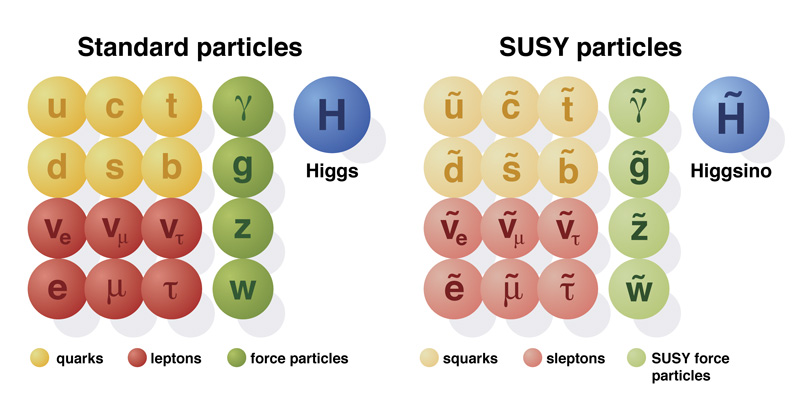
\includegraphics[width=0.85\textwidth]{figures/strategy/SUSYparticles.jpg}\hspace{0.05\textwidth}
\caption[Diagram of SM particles and their respective superpartners]{ Diagram of SM particles and their respective superpartners. }
\label{fig:SUSYpart}
%\end{center}
\end{figure}

\indent SUSY gives one possible solution to the hierarchy problem of the Higgs as large contributions to the Higgs potential are canceled out between SM particles and their superpartners.  Some supersymmetric models also unify the strong and electroweak force at high energies, provide more cp violation to generate matter/antimatter asymmetry and produce plausible dark matter candidates.  At the same time, general relativity is automatically included if SUSY is imposed as a local symmetry. This offers a potential path to uniting general relativity with quantum mechanics.  \\

\indent All previous high energy experiments including the Tevatron and LEP have not detected the existence of superpartners.  Therefore, if SUSY exists in nature then it must be a spontaneously broken symmetry.  Many different SUSY symmetry-breaking mechanisms have been proposed but they all make the superpartners more massive then their SM counterparts. \\

\indent A major goal of the Large Hadron Collider (LHC) experiment is to search for the predicted superpartners at an unprecedented energy scale.  If SUSY is the solution to the hierarchy problem and restores naturalness to the Higgs mechanism then the superpartner to the top quark (stop) is expected to be no heavier then a few $\tev$.  The stop's mass is strongly constrained due to the large coupling between the SM top quark and the Higgs with $\lambda_t \sim 0.94$.  As such, searches for the stop at the LHC is especially interesting because the stop's mass may be low enough to be directly produced at the energy scale of the LHC. \\

\indent This thesis concerns the search for stops in an traditionally experimentally difficult region.  One expected stop decay channel produces a top quark along with the superpartner to a neutral electroweak boson, the neutralino (\ninoone).  The Feynman diagram for stop production and decay is shown in figure \ref{fig:stopprod}. \\

\begin{figure}[h!]
%\begin{center}
\centering
    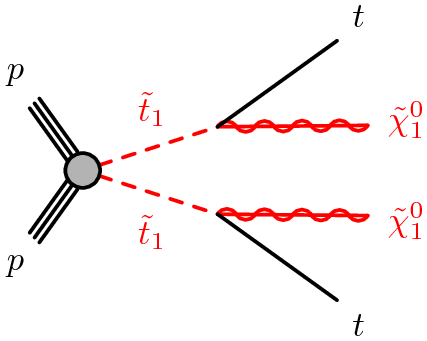
\includegraphics[width=0.45\textwidth]{figures/feynDiag/stst-tN1tN1.png}\hspace{0.05\textwidth}
\caption[Feynman diagram for the production and decay of stops at the LHC]{ Feynman diagram for the $pp \rightarrow \stop\stop \rightarrow t\ninoone t\ninoone$ process.  This process is one of the expected stop production and decay channels at the LHC.  The $\stop \rightarrow t\ninoone$ decay channel can have large branching fractions if the lightest stop is mainly right-handed or the lightest supersymmetric particle is a bino. The exact branching fraction depends on the sparticle masses in the SUSY model and whether the lightest stop is mainly right or left-handed. }
\label{fig:stopprod}
%\end{center}
\end{figure}

\indent One popular search strategy for stops targets the experimental signatures of neutralinos as they are unique to SUSY.  Experimentally this involves searching for events with large missing transverse energy ($\met$), the experimental signature of high momentum neutralinos.  This search strategy can effectively detect stops if there is a large mass splitting between $m_{\stop}$ and $m_{\ninoone}$. The heavy stop can impart large amounts of momentum onto its decay products in this region of phase space.  Monte Carlo simulation of the $\met$ distribution for the $m_{\stop} = 1000 \gev$ and $m_{\ninoone} = 1 \gev$ signal is shown as the dashed yellow histogram in figure \ref{fig:presel:MET}.  The $\met$ distribution for SM backgrounds can also be seen in the solid stacked histogram.  \\

\begin{figure}[h!]
%\begin{center}
\centering
    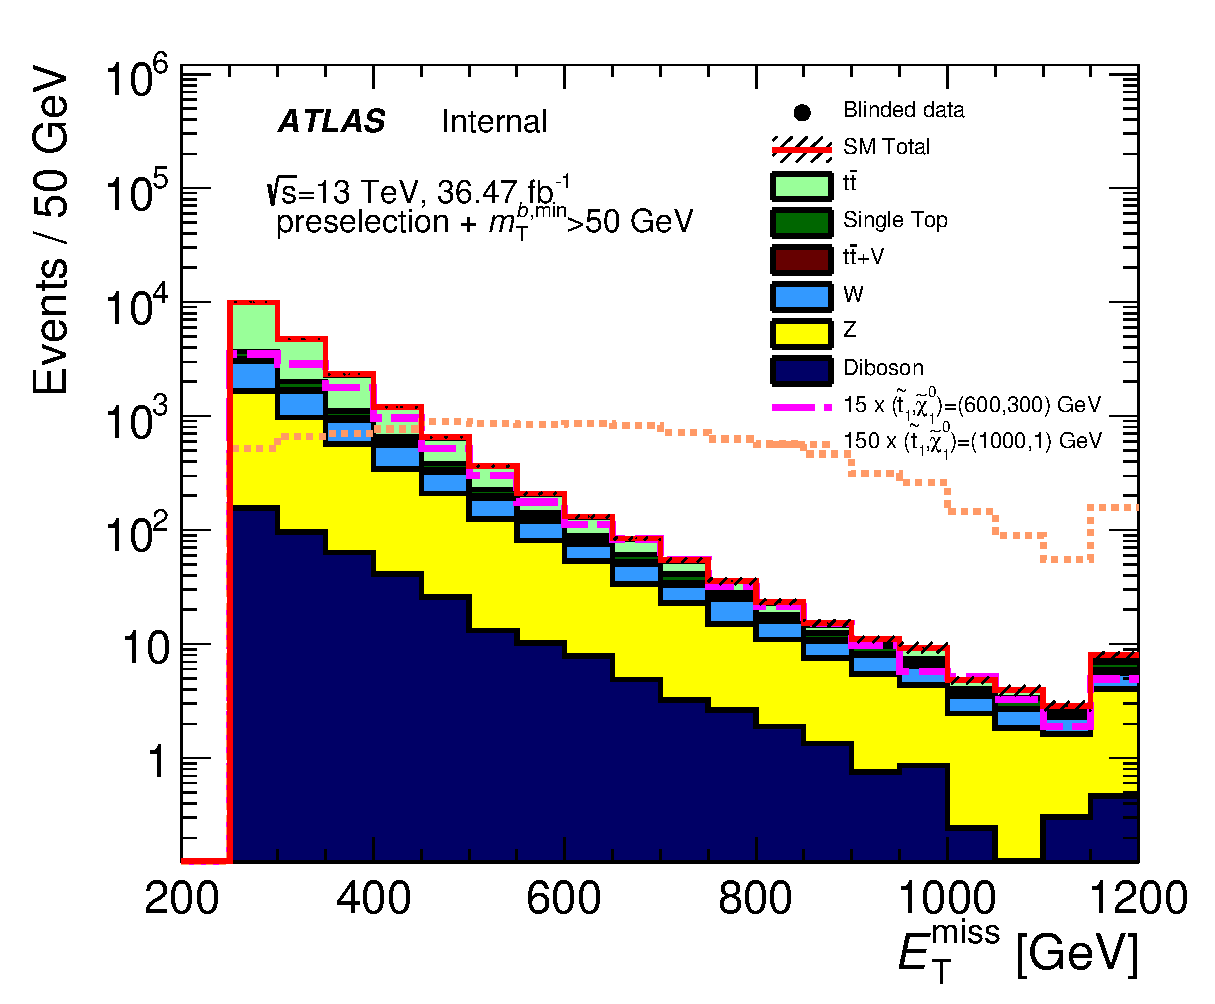
\includegraphics[width=0.85\textwidth]{figures/preselection/Met_preCutSRPlot_withRatio_log.eps}\hspace{0.05\textwidth}
\caption[Stop signal with $m_{\stop}-m_{\ninoone} >> m_t$ and SM background $\met$ distribution after loose preliminary selections for $\met>250 \gev$, zero leptons and at least four jets]{ $\met$ distribution for $(m_{\stop}, m_{\ninoone}) = (1000 \gev,1 \gev)$ and $(600 \gev, 300 \gev)$ stop signal and expected SM background.  The signal cross section has been scaled up by 150 and 15 respectively for better visibility.  Basic selections ensuring well reconstructed $\met$, no leptons, and at least four jets are applied.  Details on selections can be found in \cite{stop0LCONF} }
\label{fig:presel:MET}
%\end{center}
\end{figure}

\indent The $\met$ distribution for the $m_{\stop} = 600 \gev$ and $m_{\ninoone} = 300 \gev$ signal can also be seen in figure \ref{fig:presel:MET} as the dashed purple histogram.  The smaller mass splitting between stop and neutralino in the (600 \gev,300 \gev) sample means the stop has less energy to boost the heavy neutralino.  This leads to a softer $\met$ distribution and less separation power between signal and background.  \\

\indent   When the stop mass is nearly degenerate to $m_t + m_{\ninoone}$ the stop has just enough energy to produce the top and neutralino.  The resulting stop decay products gain little momenta from the stop decay. The low $\pt$ neutralinos in turn generate very little $\met$.  The $\met$ distribution for $(m_{\stop}, m_{\ninoone}) = (250 \gev,77 \gev)$, $(300 \gev, 127 \gev)$ and $(400 \gev, 227 \gev)$ signal samples is given in figure \ref{fig:presel:MET_diag}.  As we can see, the $\met$ variable provides little separation power between signal and background in this region of phase space. \\

\begin{figure}[h!]
%\begin{center}
\centering
    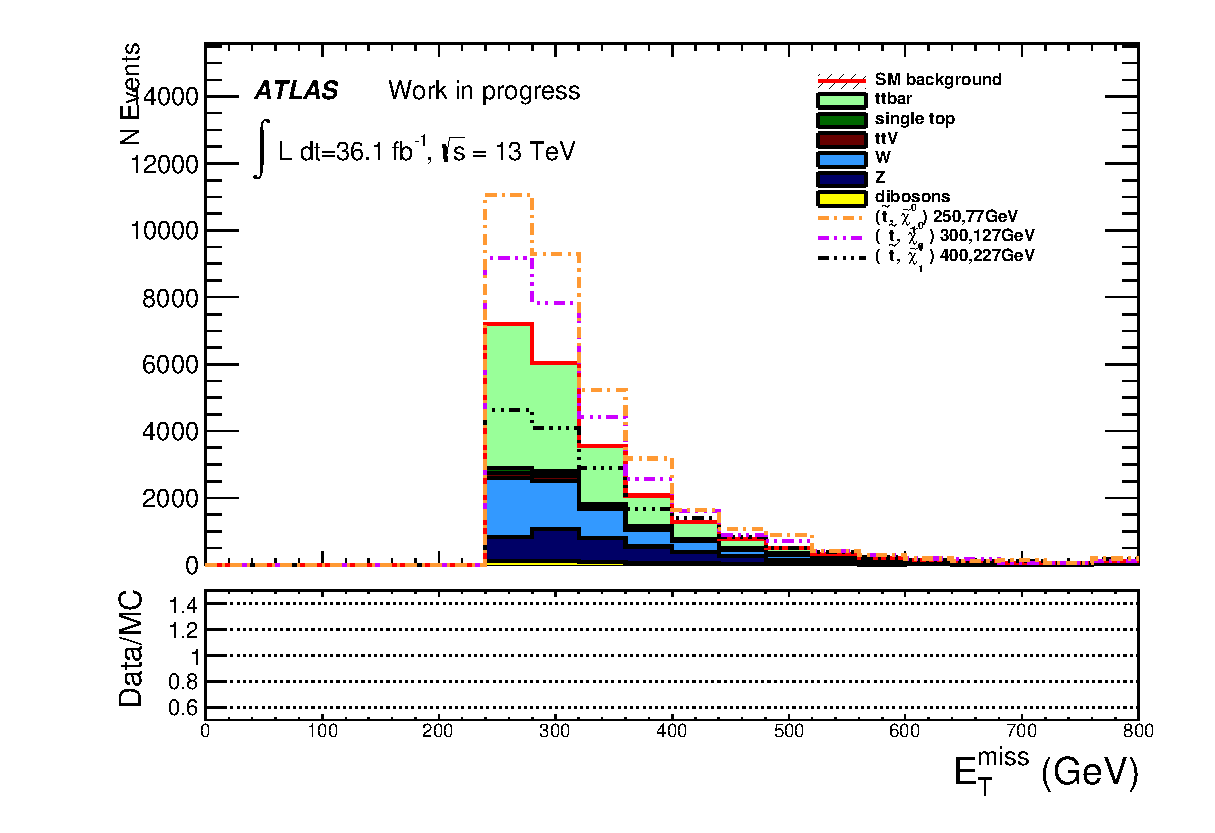
\includegraphics[width=0.85\textwidth]{figures/plotSR/SR_eT_miss_0SR.eps}\hspace{0.05\textwidth}
\caption[Stop signal with $m_{\stop}-m_{\ninoone} \sim m_t$ and SM background $\met$ distribution after loose preliminary selections for $\met>250 \gev$, zero leptons and at least four jets]{ $\met$ distribution for $(m_{\stop}, m_{\ninoone}) = (250 \gev,77 \gev)$, $(300 \gev, 127 \gev)$ and $(400 \gev, 227 \gev)$ stop signal and expected SM background.  All three signal samples have $m_{\stop}-m_{\ninoone} \sim m_t$.  The signal cross section has also been scaled up by a factor of 20 for better visibility.  Basic selections ensuring well reconstructed $\met$, no leptons, and minimal jet multiplicity requirements are applied.  Preselections are defined in chapter \ref{chap:Selection_EventPreselection} }
\label{fig:presel:MET_diag}
%\end{center}
\end{figure}

\indent The only other observables in the event are the visible tops which are also produced in SM top/anti-top pair (ttbar) production.  This inability to distinguish SM ttbar from stop signal greatly hamper the search sensitivity in this region because SM ttbar production cross section is 50$\times$ to 300$\times$ that of the stop . \\

\indent The low decay product $\pt$ problem is ubiquitous to all regions of phase space with small mass splittings.  Many ATLAS searches in SUSY including charginos, Higgsinos, sbottom, sleptons, etc all have some region of phase space with a compressed mass spectra.  In general, such regions of phase space are called compressed regions. \\

\indent The ATLAS Run 1 stop search results are summarized in figure \ref{fig:ATLAS:8TeVResult}.  Shaded regions have been excluded by ATLAS Run 1 searches to 95\% confidence.  The different colored regions correspond to different searches.  \\

\begin{figure}[h!]
%\begin{center}
\centering
    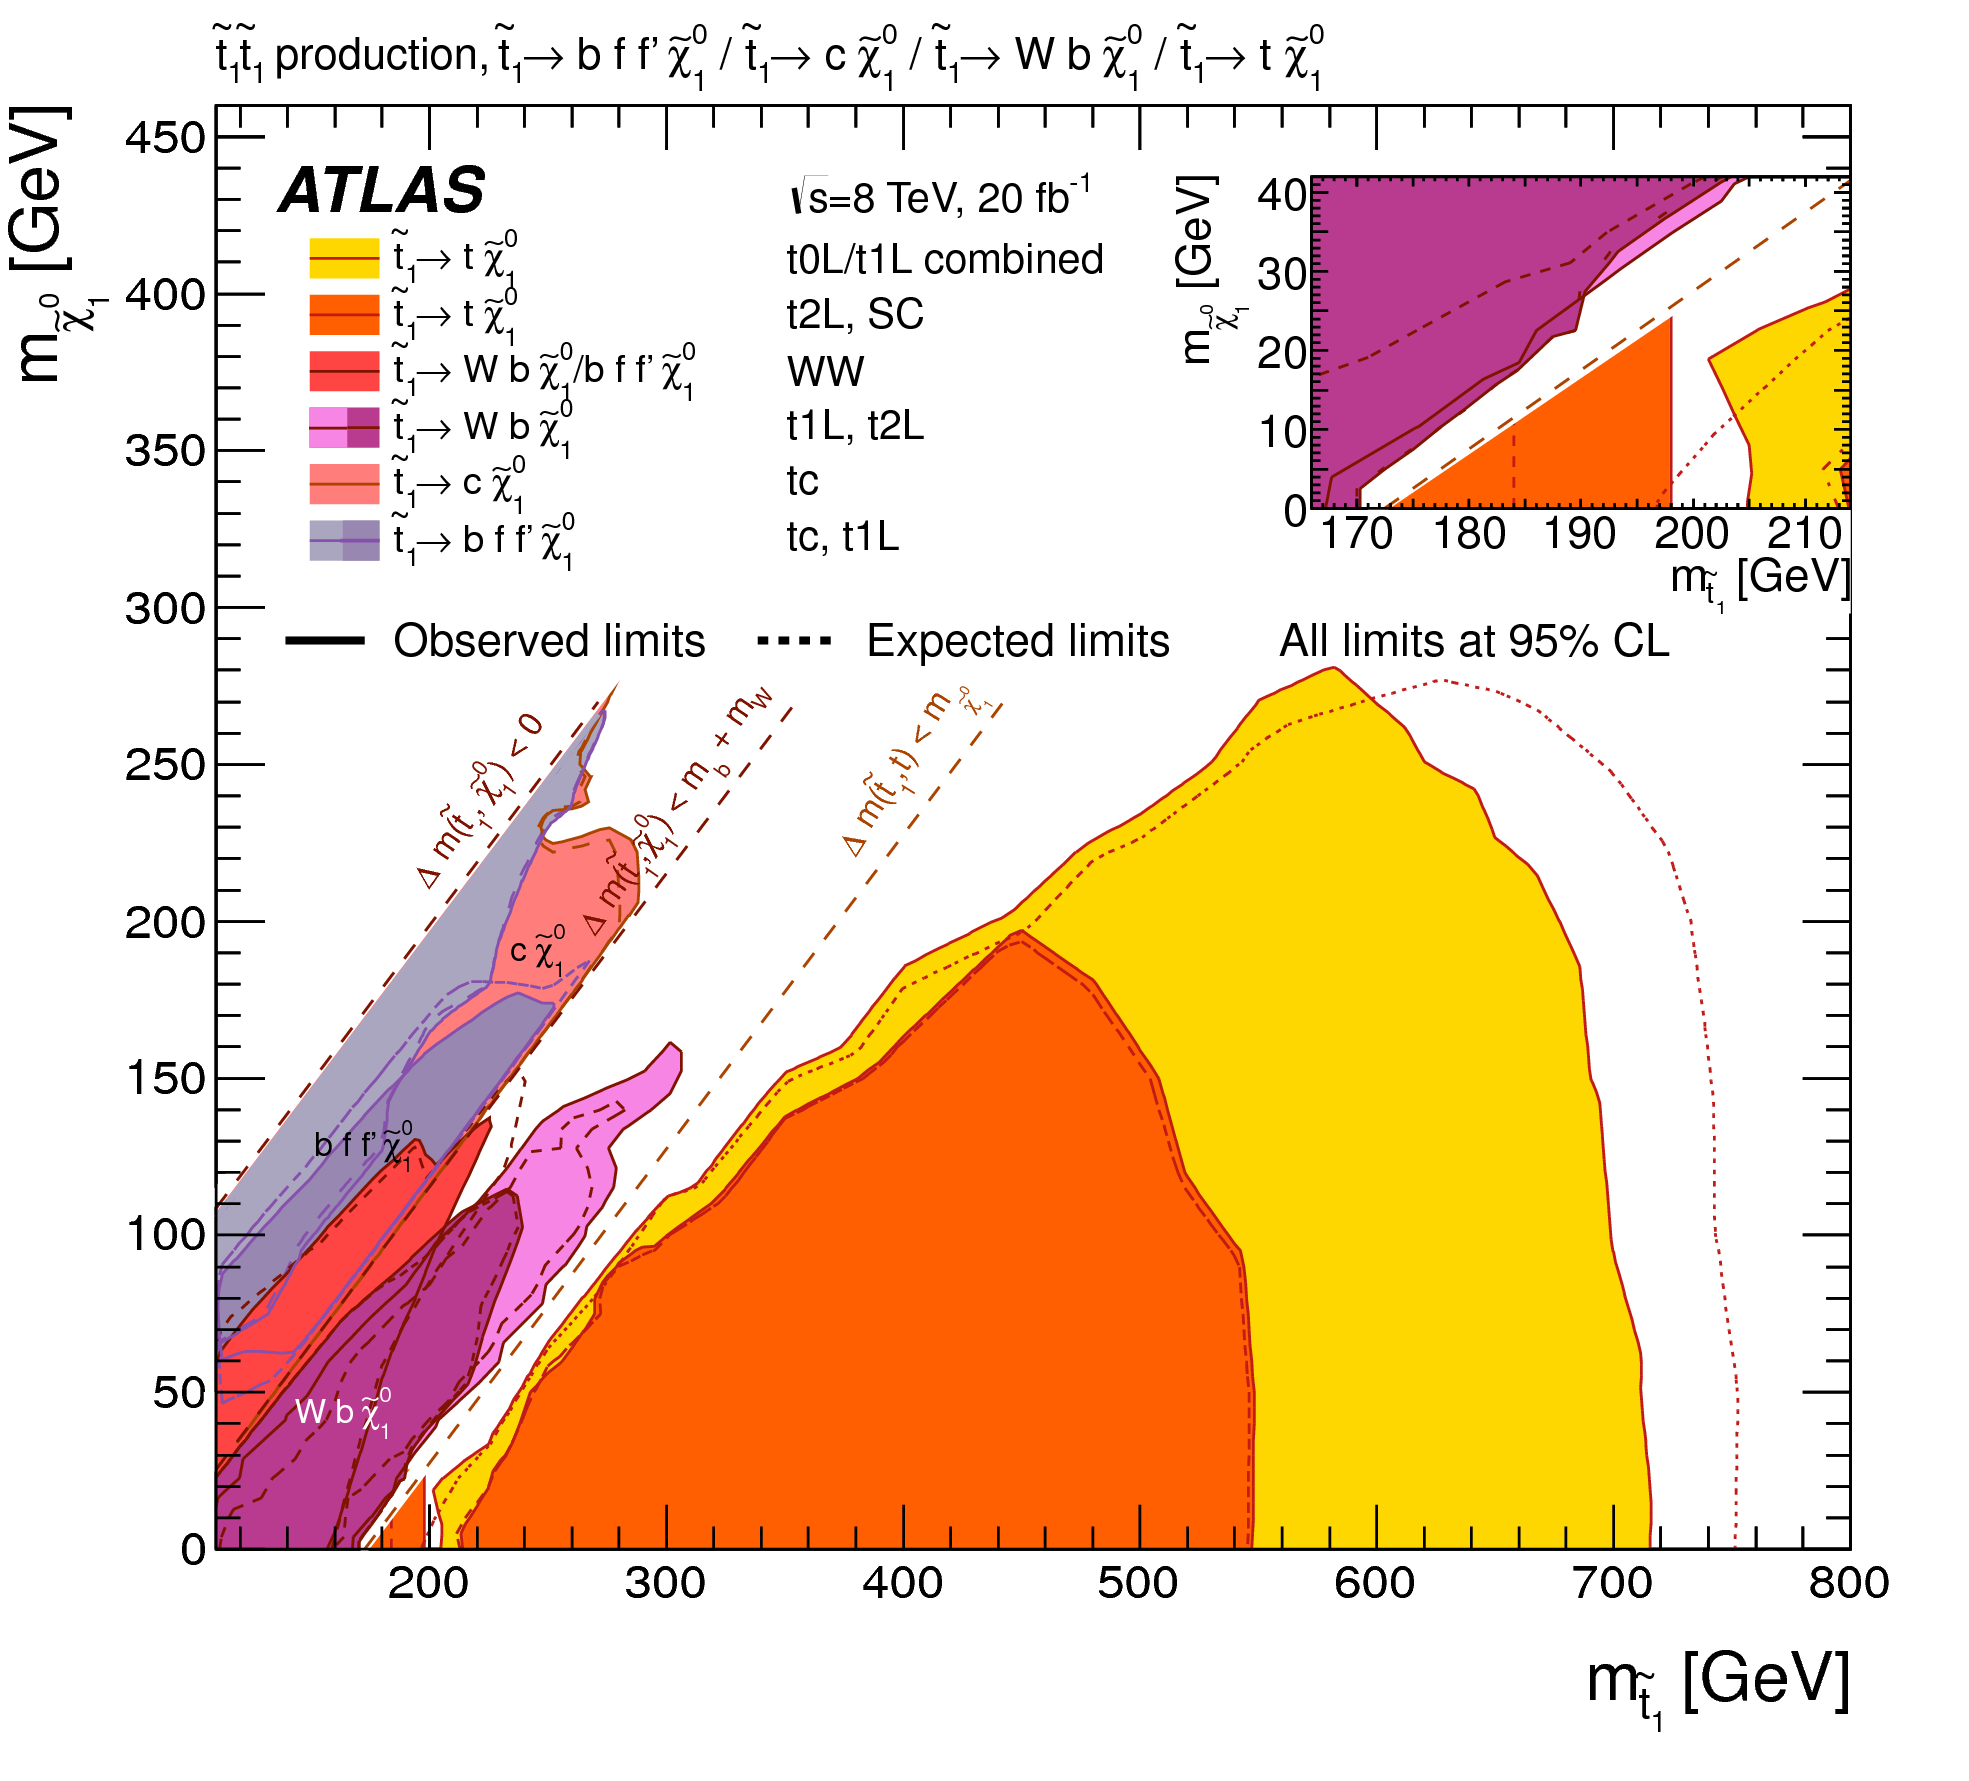
\includegraphics[width=0.85\textwidth]{figures/8TeV/ATLAS_SUSY_Stop_tLSP_201507.png}\hspace{0.05\textwidth}
\caption[95\% confidence limits on stop parameter space from various analysis on ATLAS $\sqrt{s} = 7+8 \tev$ data]{ 95\% confidence limits on stop parameter space from various analysis on ATLAS $\sqrt{s} = 7+8 \tev$ data.  Shaded regions have been excluded by ATLAS Run 1 searches.  Different colored regions correspond to different search strategies including different experimental signatures. The $m_{\stop}-m_{\ninoone} = m_t$ remains unconstrained for all stop masses. }
\label{fig:ATLAS:8TeVResult}
%\end{center}
\end{figure}

\indent Searches targeting high $\met$ is sensitive to stop signals with large mass splittings at the bottom right corner. Searches targeting off shell top decays are sensitive to regions with mass splittings smaller than the top mass ($m_{\stop}-m_{\ninoone} < m_t$).  These searches are able to rule out the purple, red and gray regions above the $m_{\stop}-m_{\ninoone} = m_t$ diagonal line.  However, the corridor near $m_{\stop}-m_{\ninoone} = m_t$ remain unconstrained even at low stop masses.  The same features can be seen in Run 1 CMS results shown in figure \ref{fig:CMS:8TeVResult}. \\

\begin{figure}[h!]
%\begin{center}
\centering
    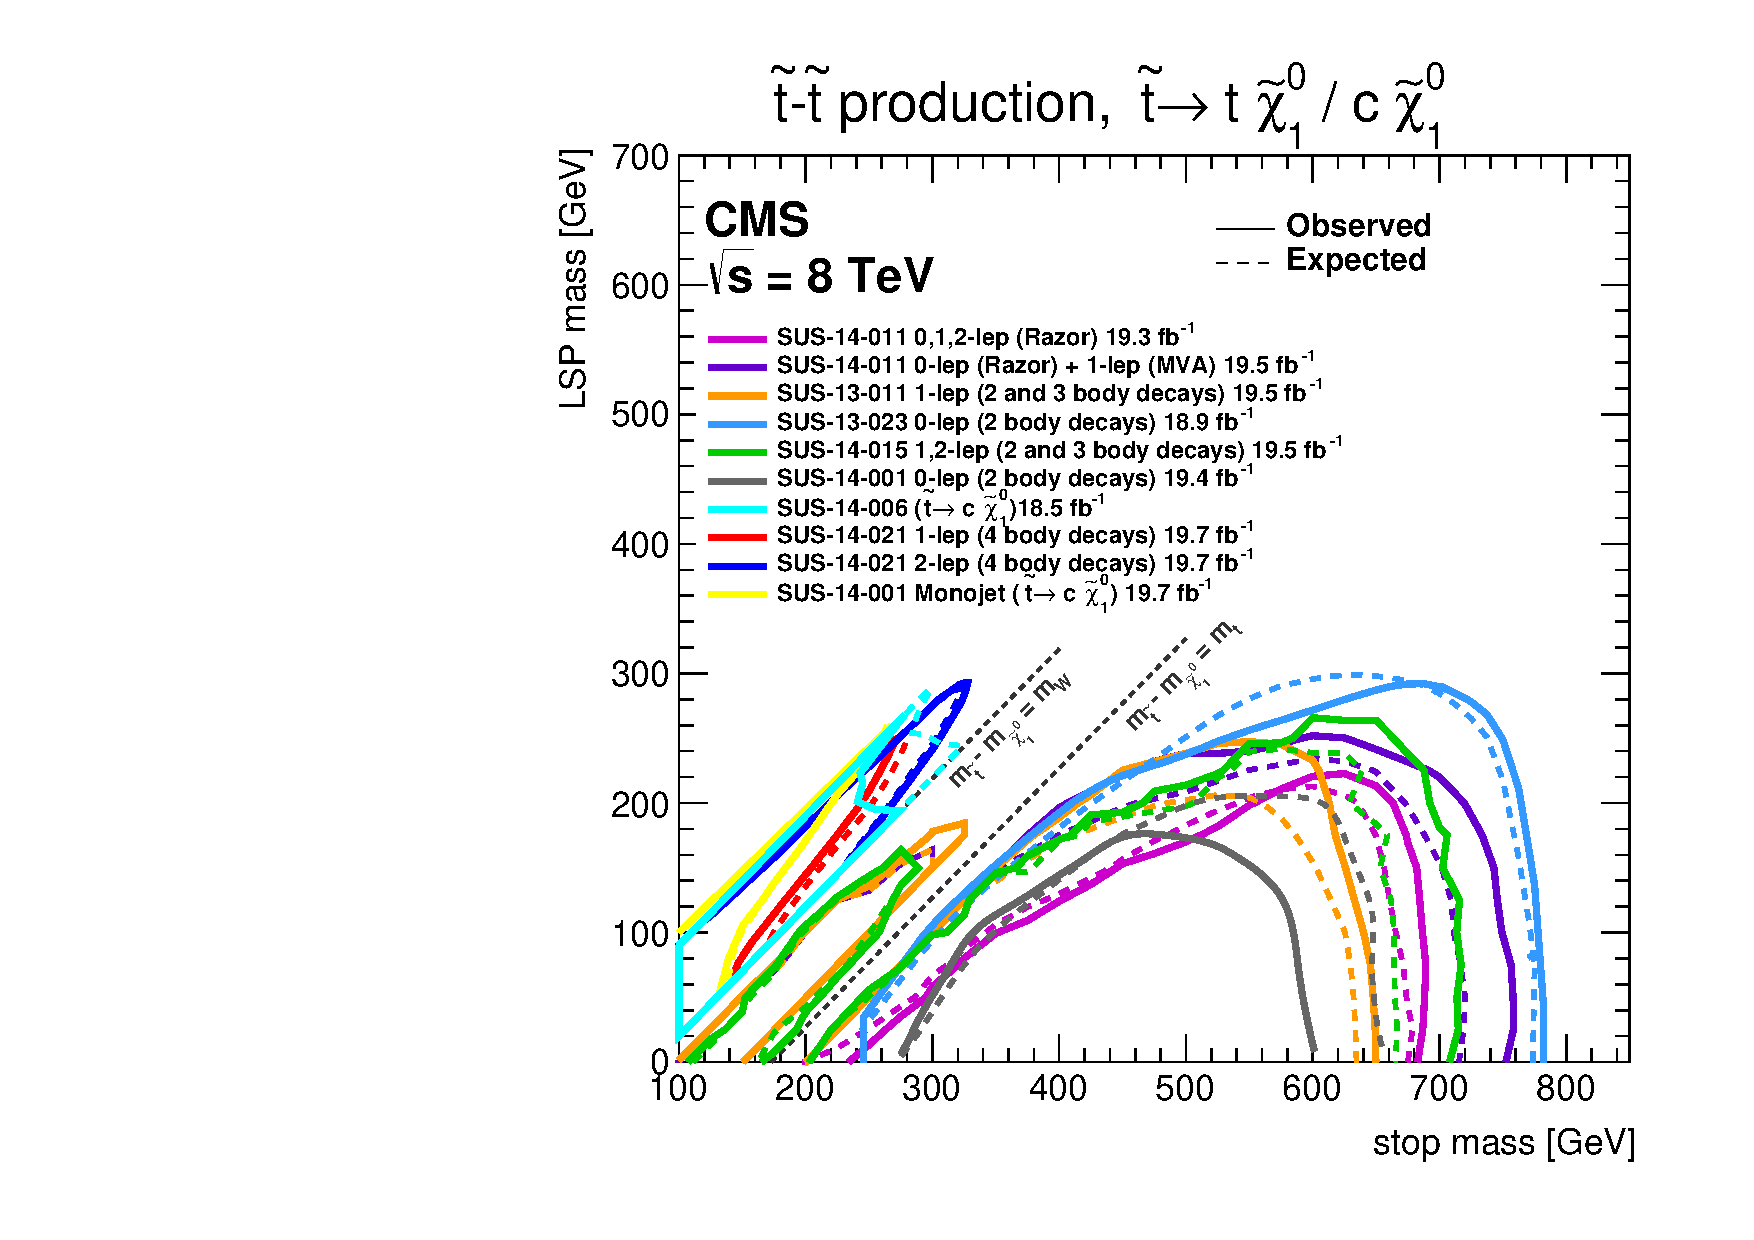
\includegraphics[width=0.85\textwidth, angle=270]{figures/8TeV/T2tt_2015.pdf}\hspace{0.05\textwidth}
\caption[95\% confidence limits on stop parameter space from various analysis on CMS $\sqrt{s} = 7+8 \tev$ data]{ 95\% confidence limits on stop parameter space from various analysis on CMS $\sqrt{s} = 7+8 \tev$ data.  Regions below colored curves have been excluded by CMS Run 1 searches.  Different colored curves correspond to different search strategies including different experimental signatures. The $m_{\stop}-m_{\ninoone} = m_t$ line remains unconstrained for all stop masses.  }
\label{fig:8TeVResult}
%\end{center}
\end{figure}


\indent This thesis demonstrates a new method of searching for stops in the $m_{\stop}-m_{\ninoone} = m_t$ compressed region by isolating events with strong initial state radiation (ISR).  The ISR boosts the stops and gives additional momentum to the stop decay products.  The correlation between ISR pt and stop decay product $\pt$ tend to be extremely strong in this region precisely because the stop decay products gain little momentum from the stop decays.  Specifically there exists a strong correlation between ISR and neutralino systems in both direction and $\pt$.  \\

\indent The neutralinos will inherit a fraction of the original ISR $\pt$ proportional to  $m_{\ninoone}/m_{\stop}$ and the two should be back-to-back.  The $\met/\PTISR$ ratio distribution can be seen in figure \ref{fig:trueRISR}.  The two stop signals both have $m_{\stop}-m_{\ninoone} = m_t$.  Their $\met/\PTISR$ ratios peak sharply at $m_{\ninoone}/m_{\stop}$ according to their respective stop and neutralino masses.  \\

\begin{figure}[h!]
%\begin{center}
\centering
    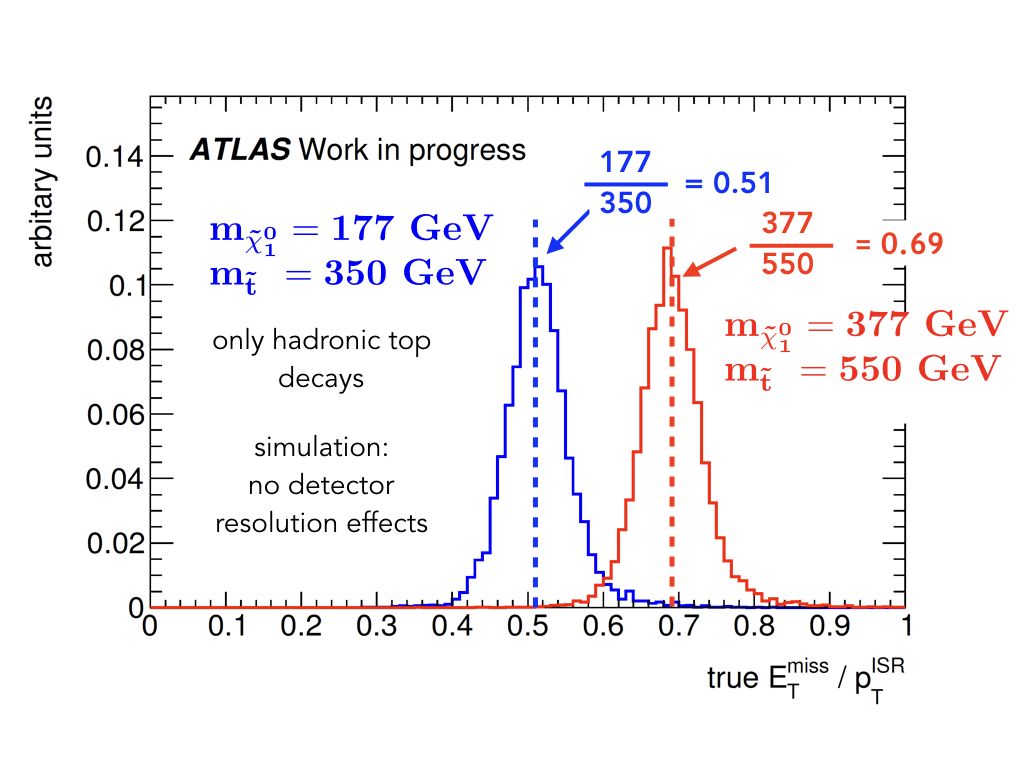
\includegraphics[width=0.85\textwidth]{figures/strategy/RISR_truth.png}\hspace{0.05\textwidth}
\caption[Correlation between the $\met/\PTISR$ ratio in simulation for stop samples with $m_{\stop}-m_{\ninoone} = m_t$]{ Correlation between the $\met/\PTISR$ ratio in simulation for two stop samples with $m_{\stop}-m_{\ninoone} = m_t$.  Both stop samples peak sharply at $m_{\ninoone}/m_{\stop}$ with only a gaussian width of 4 percent.  Deviation from the preferred ratio is limited by the top width, as the top must be pulled off-shell to generate phase space. No detector resolution effects where included and only the all hadronic decay channel was considered. }
\label{fig:trueRISR}
%\end{center}
\end{figure}

\indent These correlations between ISR and $\met$ allow us to separate signal from ttbar background and overcome the difference in production cross section in this experimentally difficult region.  \\

\indent In order to capitalize on these sharply peaking variables, we developed a new accurate ISR identification system.  The algorithm works by first finding the axis of maximum back-to-back $\pt$ call the thrust axis.  The thrust axis should mimic the axis of back-to-back boost between the ISR and sparticle systems in events with strong ISR because the ISR and sparticle boost represents the single largest back-to-back kick in events with strong ISR.  \\

\indent A schematic representation of the thrust axis in stop plus strong ISR events can be seen in figure \ref{fig:ISR:ttbar_sig_example}. \\

\begin{figure}[h!]
  \centering
	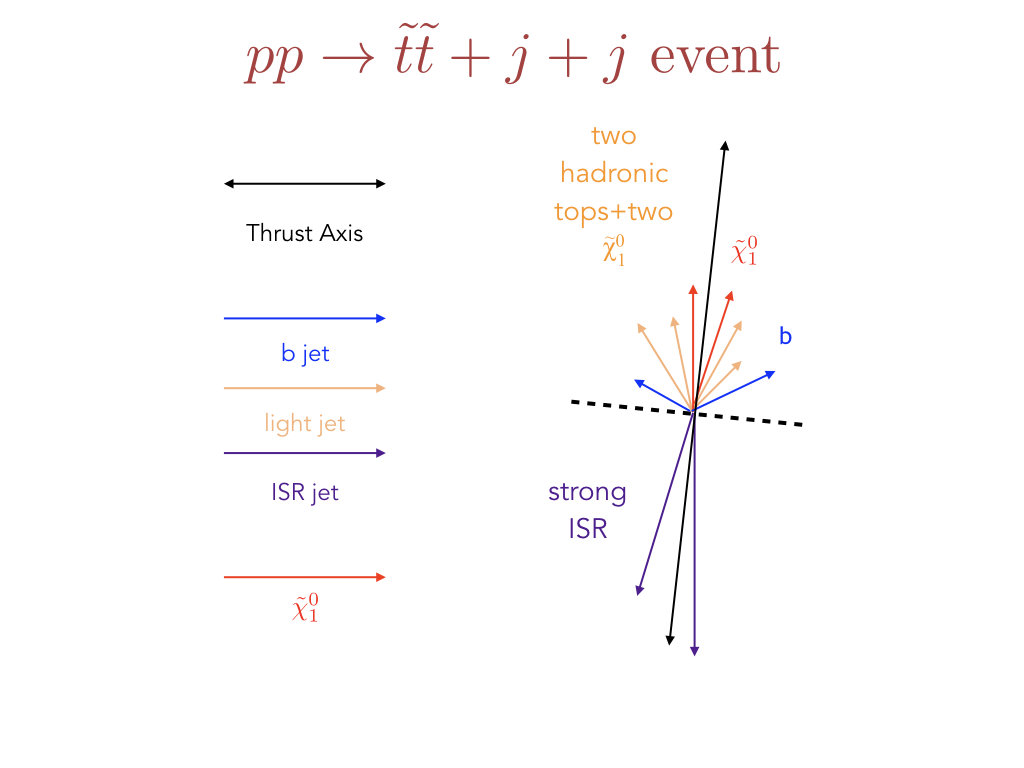
\includegraphics[width=0.85\textwidth]{./figures/strategy/ISR_signal.png}
	\caption[Schematic depictions of stop plus strong initial state radiation event kinematics]{Schematic depictions of stop plus strong ISR event kinematics.  The thrust axis approximates the direction of back-to-back boost between ISR and stop decay products.  The hemisphere containing $\met$ also contains most of the other stop decay products.  The hemisphere opposite the $\met$ contains the energetic ISR jets. }
	\label{fig:ISR:ttbar_sig_example}
\end{figure}

\indent We then divide the event into two hemispheres according to the thrust axis.  All objects in the same hemisphere as the $\met$ are considered to have originated from a stop decay because we expect the neutralinos to travel in the same direction as the original stops.  All objects in the hemisphere opposite the $\met$ are considered to have originated from ISR.  In this way, the thrust-based algorithm is able to identify entire ISR systems composed of multiple jets.  \\ 

\indent The ISR identification algorithm is completely general and can be used to identify ISR for SM processes as well as other BSM searches.  The performance of the ISR identification algorithm in stop and SM ttbar events can be seen in figure \ref{fig:ISRPerformanceIntro}.  In summary, the algorithm can achieve a 9 percent uncertainty on the reconstructed ISR $\pt$ in stop and ttbar events with at least 400 $\gev$ of true ISR $\pt$. This uncertainty includes any detector uncertainties due to the reconstruction of jets, $\met$ and other physics objects.  \\

\begin{figure}[h]
\centering
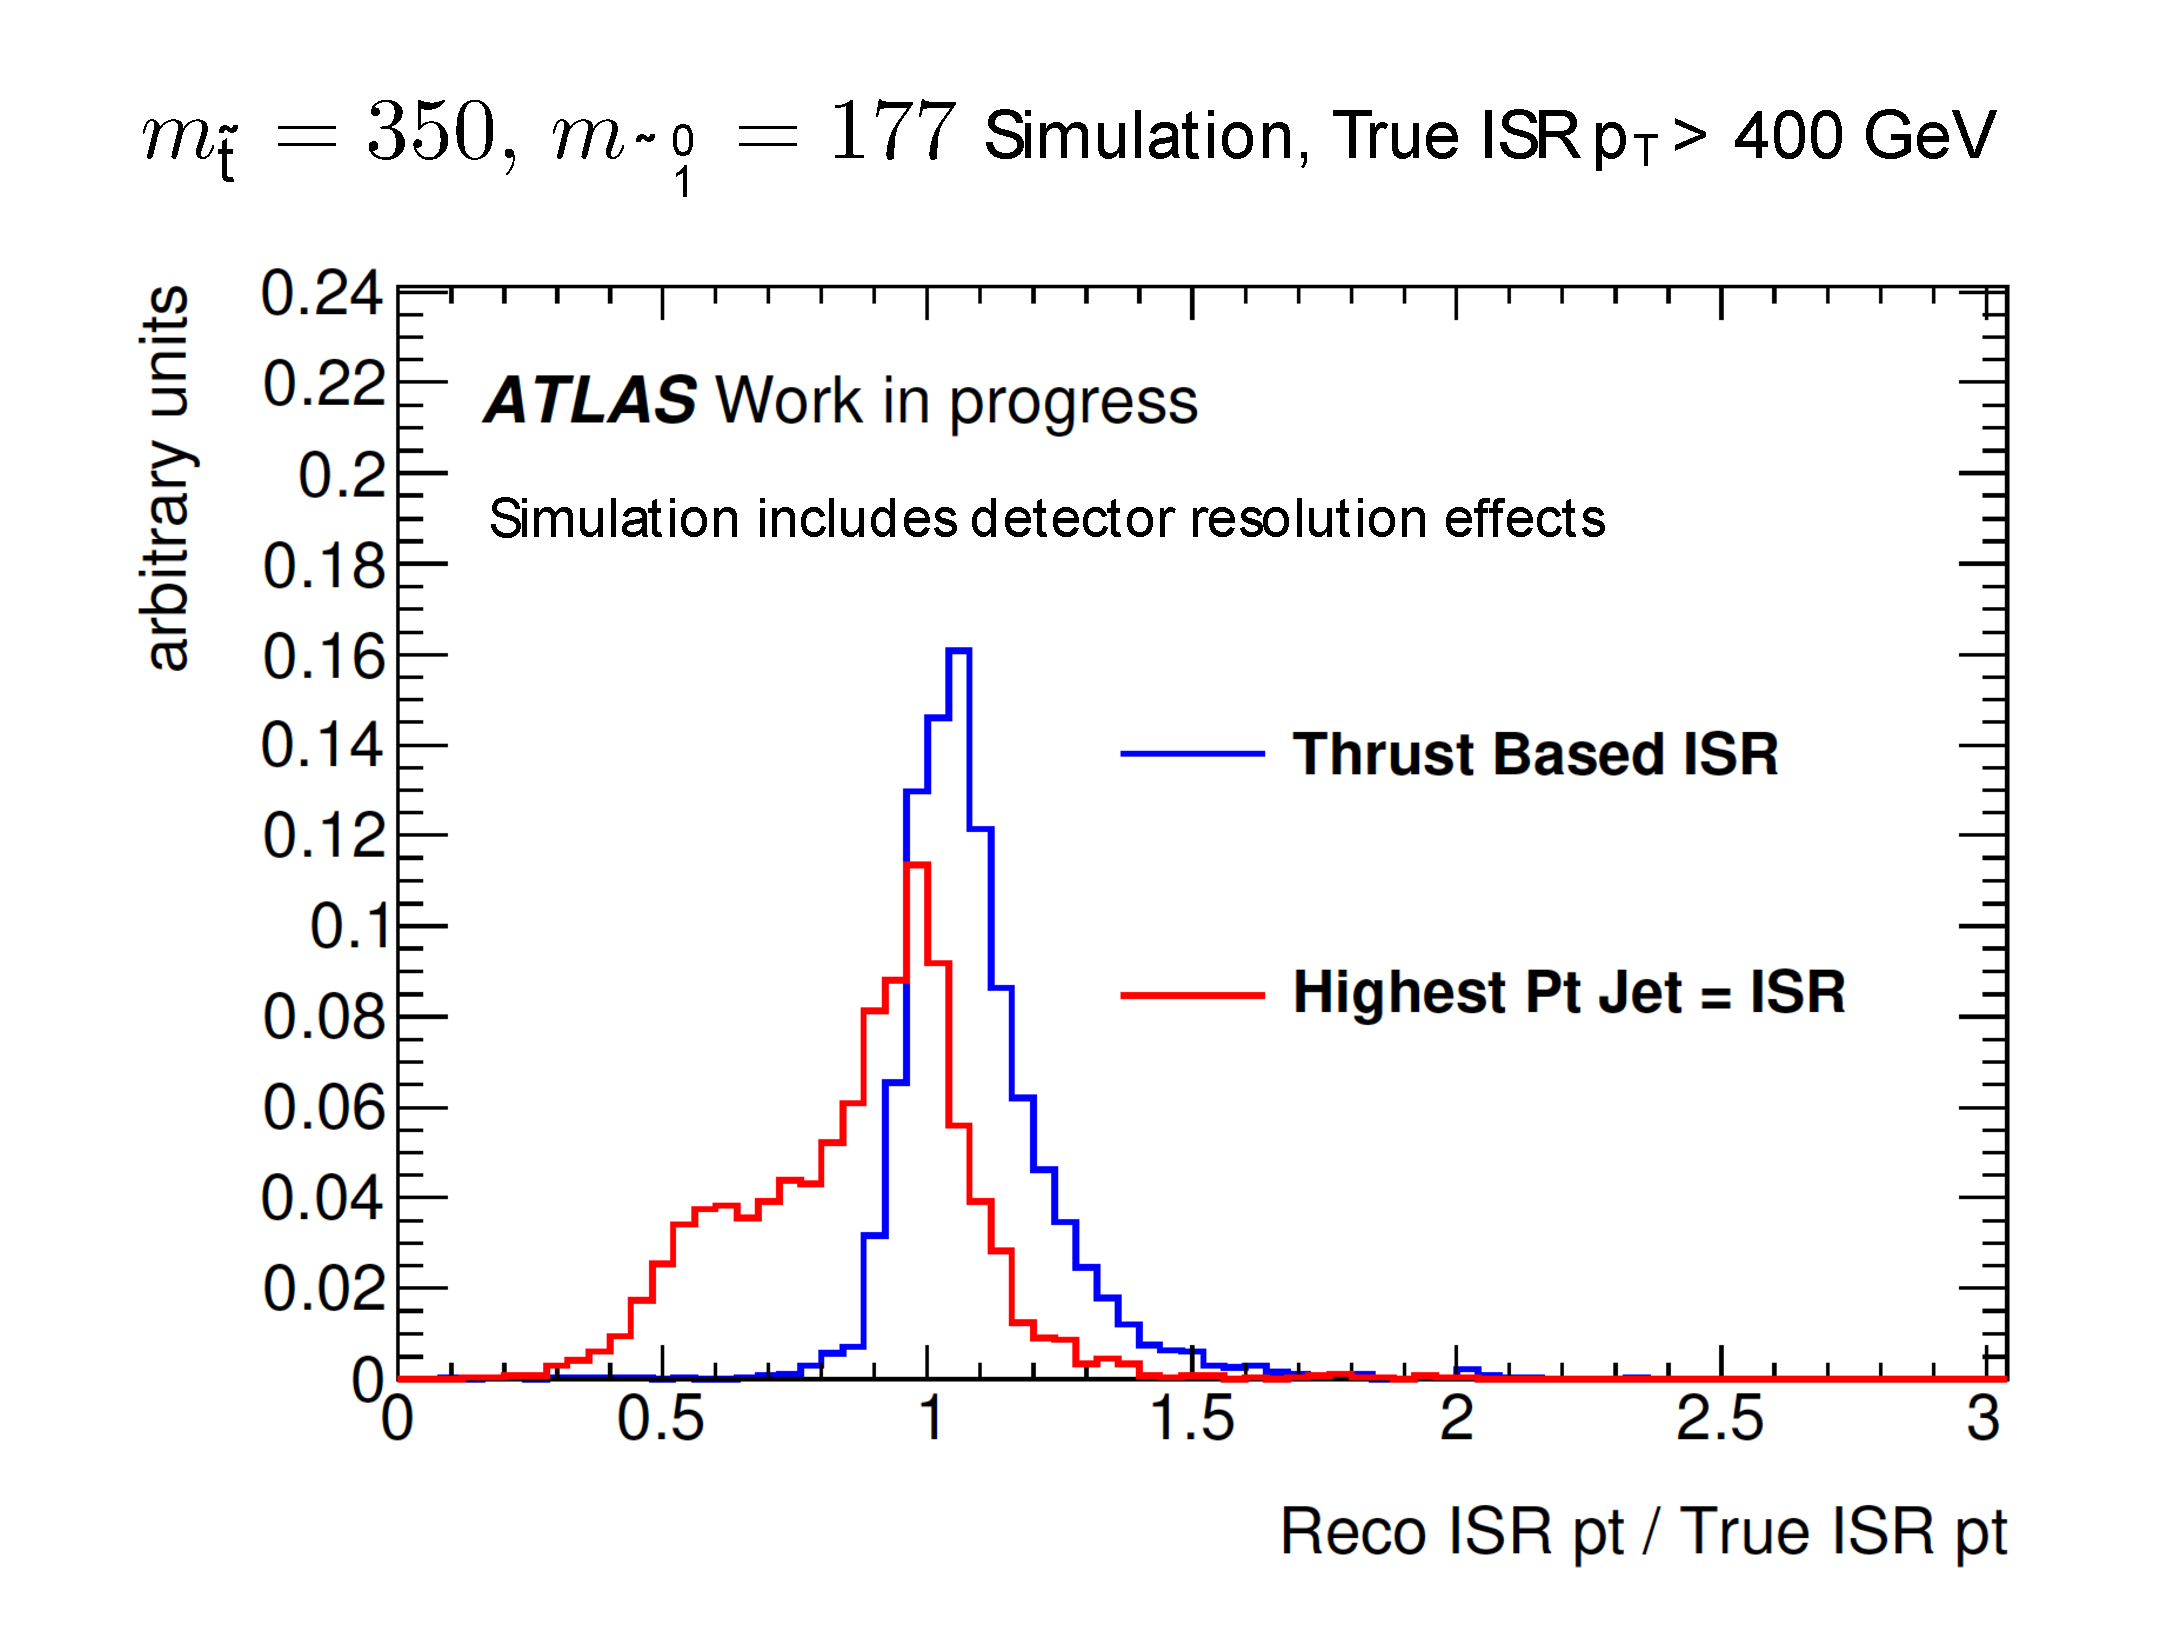
\includegraphics[width=0.45\textwidth]{./figures/strategy/ThrustAlgoEfficiency.eps}
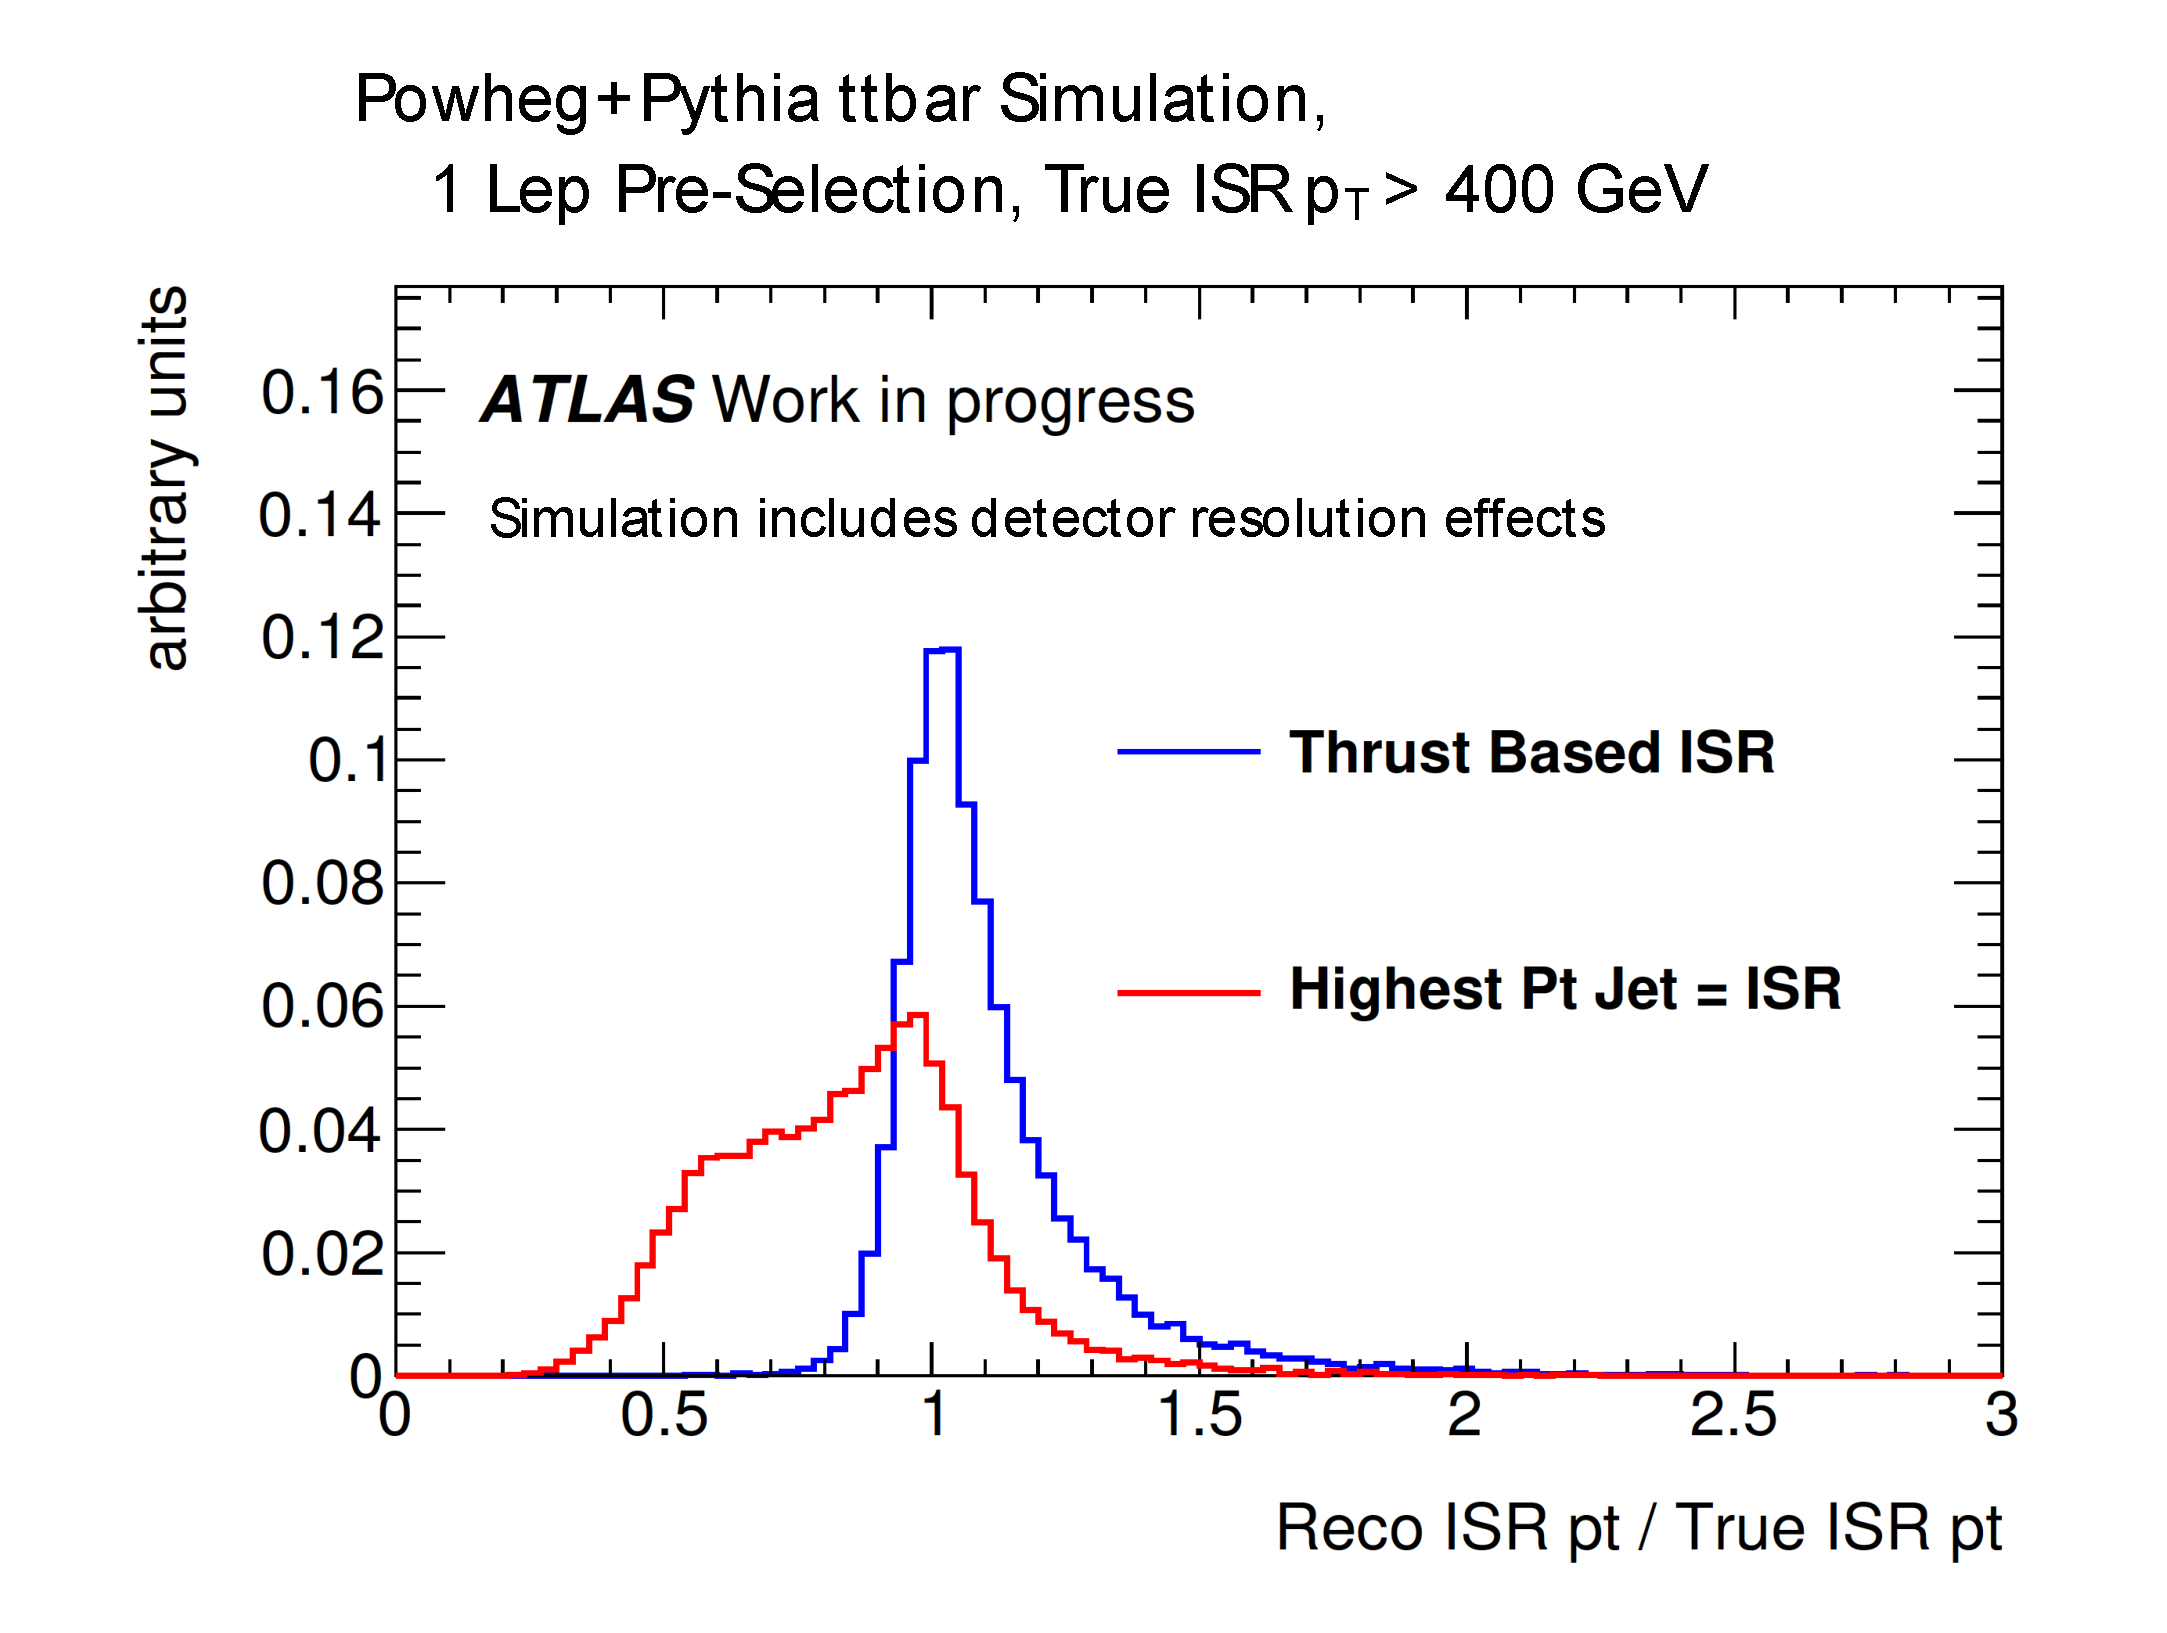
\includegraphics[width=0.45\textwidth]{./figures/strategy/ThrustAlgoEfficiency_ttbar.eps}
\caption[Distributions of the reconstructed ISR $\pt$ over true ISR $\pt$ ratio for stop signal and ttbar background in simulation]{Distributions of the reconstructed ISR $\pt$ over true ISR $\pt$ ratio for stop signal and ttbar background in simulation.  Only events with at least $400$ GeV of true ISR $\pt$ are accepted.  The red distribution is formed when the whole ISR system is equated to just the highest $\pt$ jet.  The blue distribution uses the thrust based ISR identification system. Detector resolution effects are included in the simulation. }
 \label{fig:ISRPerformanceIntro}
\end{figure}

\indent The ISR based search has allowed us to finally make a definitive statement on the existence of stops in a region with no previous exclusion sensitivity.  Using the $\intlumi$ $\ifb$ 2015 and 2016 $\sqrt{s}=13 \tev$ dataset, we were able to exclude stops in this compressed region with masses between 225 and 600 $\gev$ to 95 percent confidence.  We were able to achieve expected exclusion confidence limits of less then $5 \times 10^{-4}$ for stop masses between 250 and 400 $\gev$.  \\

\indent The 95\% confidence limit for the analysis is shown in figure \ref{figure.exclusion.All2016}.  The compressed analysis is responsible for the orange region covering the $m_{\stop}-m_{\ninoone} = m_t$ diagonal line.  The compressed analysis also has sensitivity to much of the region between $m_{\stop}-m_{\ninoone} = m_W + m_b$ and $m_{\stop}-m_{\ninoone} = m_t + 30 \gev$.  The sensitivity to this diagonal line complements the two lepton search in purple to the left and the zero lepton high mass splitting search to the right.  \\

\begin{figure}[htbp]
	\begin{center}
		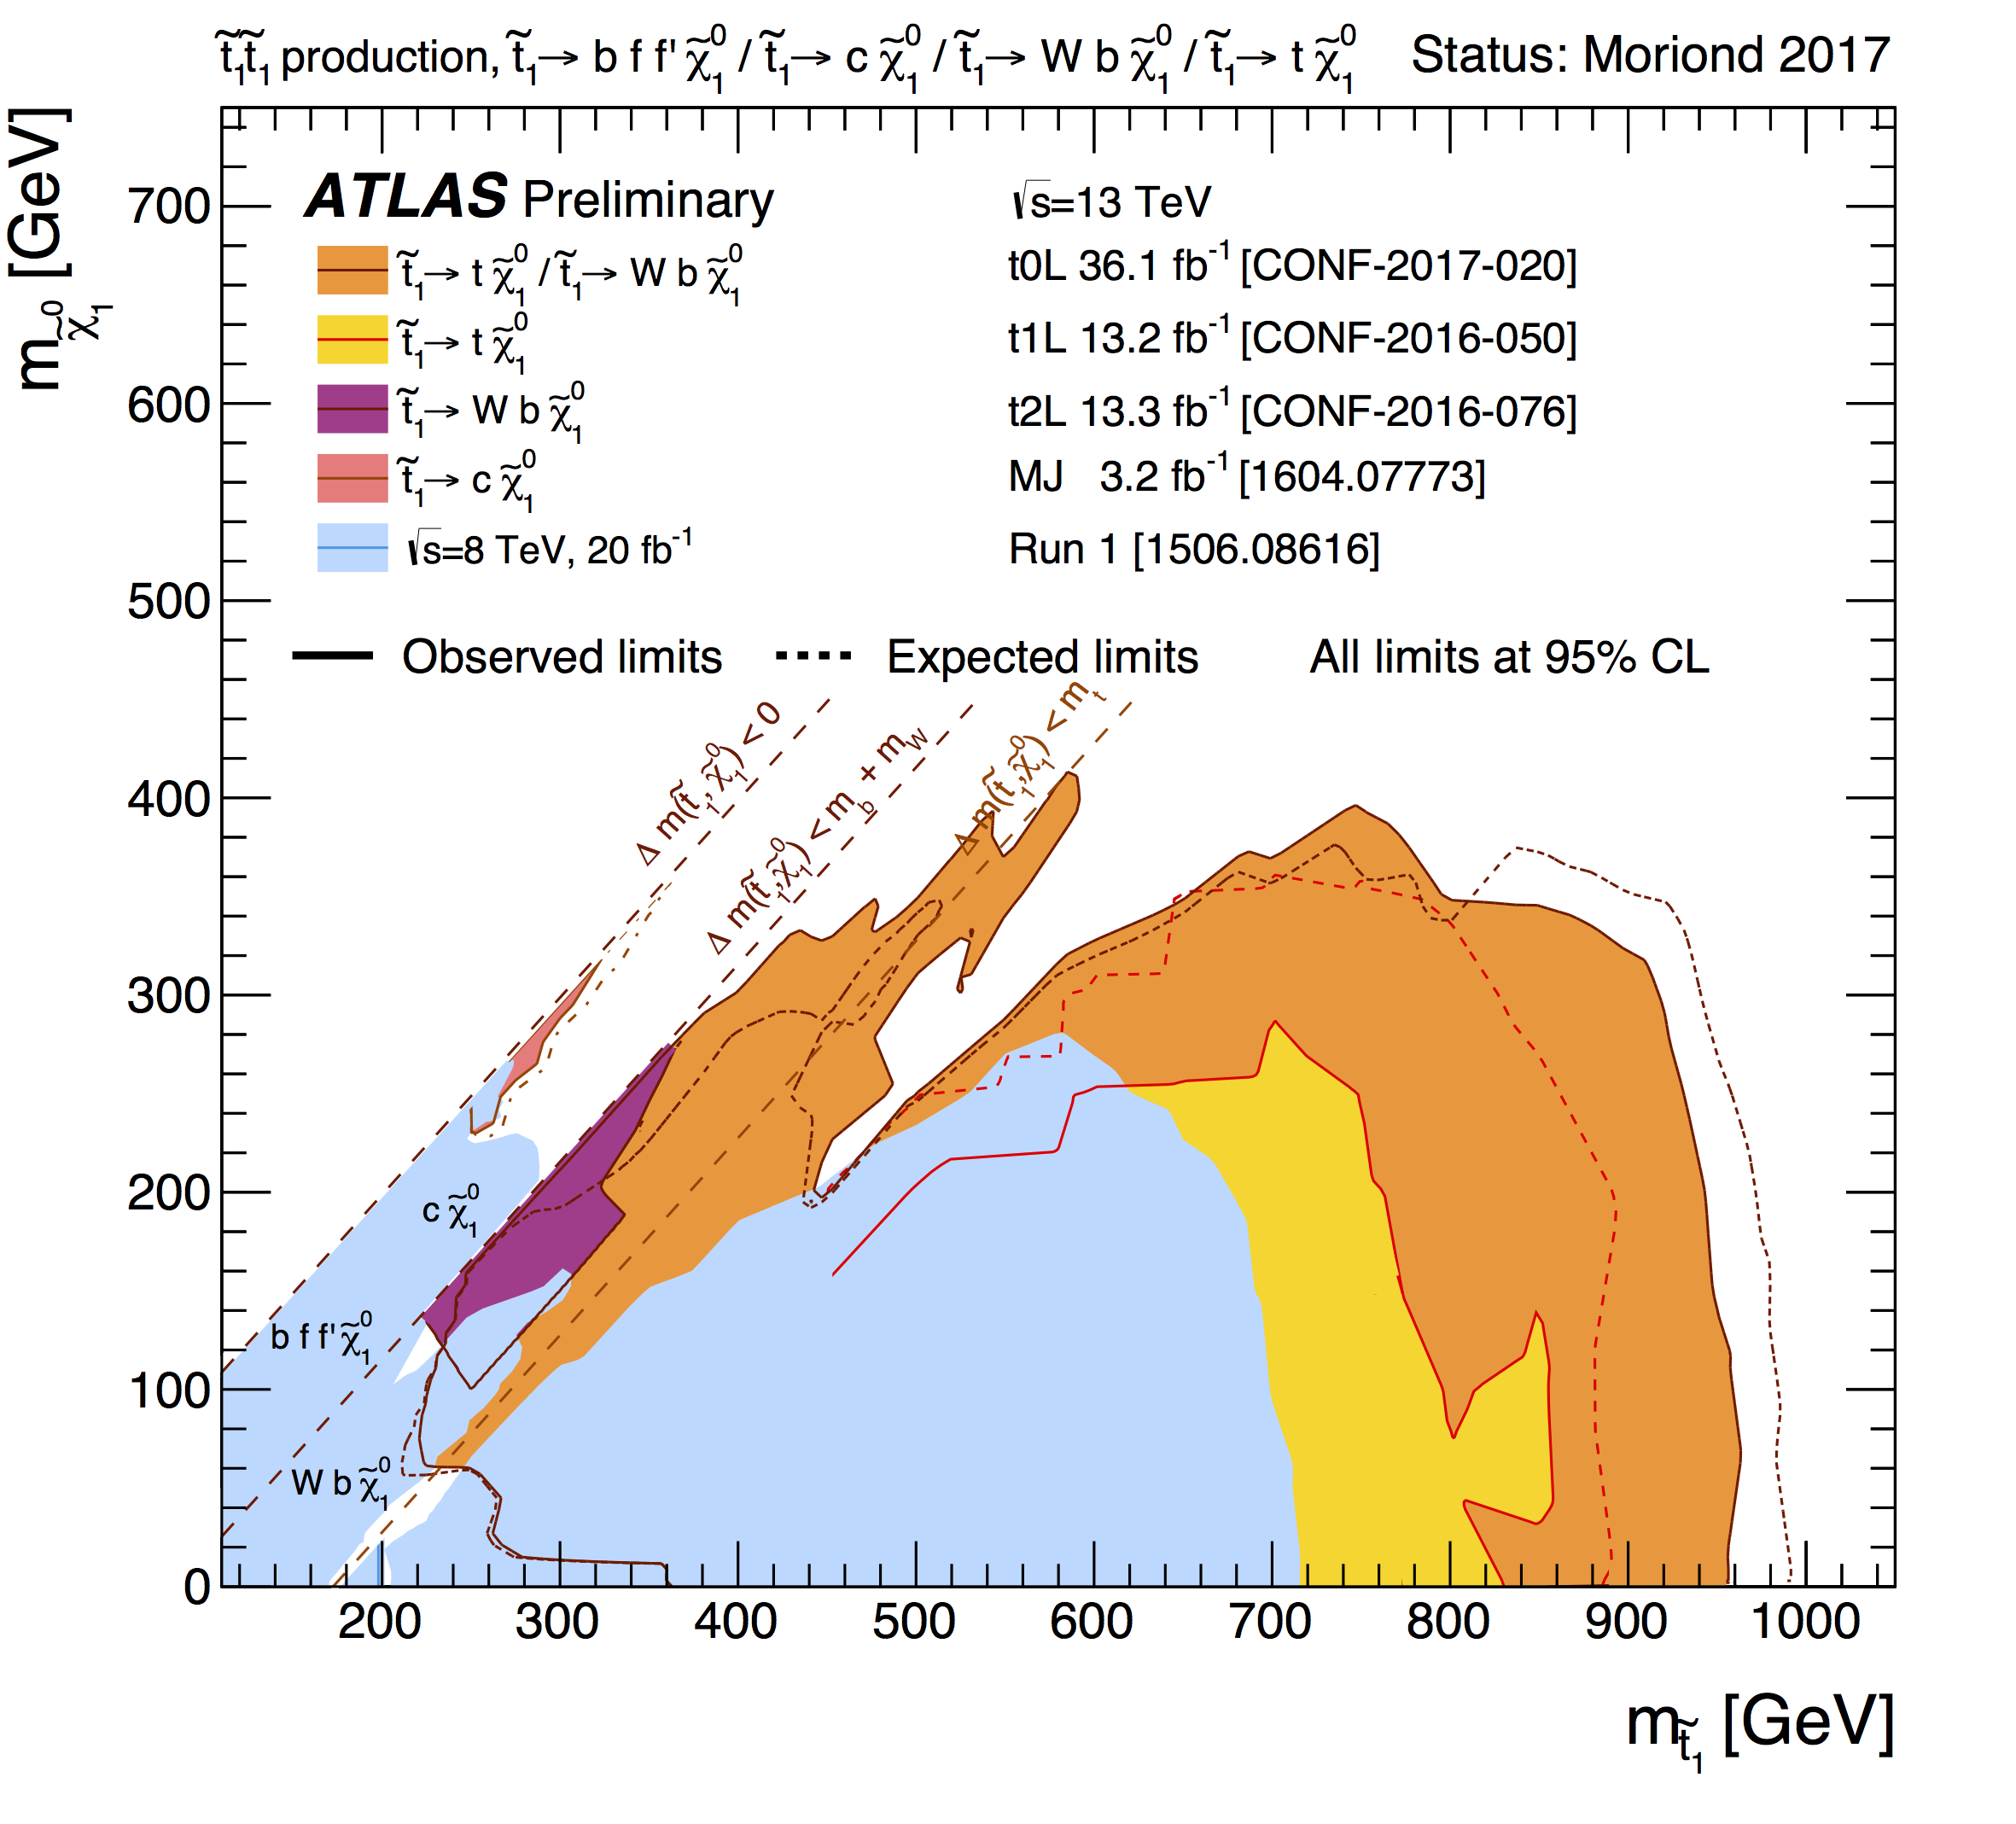
\includegraphics[width=0.85\textwidth]{figures/8TeV/ATLAS_SUSY_Stop_tLSP.png}
		\caption[95\% confidence limit on stop parameter space resulting from all ATLAS stop searches on the 2015+2016 dataset]{95\% confidence limit on stop parameter space resulting from all ATLAS stop searches on the 2015+2016 dataset.  The compressed analysis is responsible for the orange region covering much of the $m_{\stop}-m_{\ninoone} = m_t$ diagonal line.  The compressed analysis also has sensitivity to much of the region between $m_{\stop}-m_{\ninoone} = m_W + m_b$ and $m_{\stop}-m_{\ninoone} = m_t + 30 \gev$.  The compress analysis covers the region between the 2 lepton analysis in purple and zero lepton high mass splitting search that is also in orange and covers stop mass to 950 $\gev$.  8 $\tev$ ATLAS results are shown in light blue for comparison.  }
		\label{figure.exclusion.All2016}
	\end{center}
\end{figure}

\indent The methods demonstrated in this thesis can be applied to other compressed region searches and searches involving ISR such as dark matter searches.  The accurate ISR identification algorithm can also directly measure the amount of ISR produced in conjunction with SM particles. Potential applications include measuring the SM ttbar ISR $\pt$ spectrum. \\

\indent  The increase in center-of-mass energy from 8 to 13 TeV translates to approximately an order of magnitude increase in the production cross section of heavy sparticles with strong ISR.  The 13 TeV dataset presents a golden opportunity to search for many experimentally difficult physics processes that need a boost from strong ISR in order to be detected. \\

\indent The thesis is organized as follows.  Chapter \ref{chap:motivation} presents an overview of the standard model and theoretical motivations for supersymmetry. Chapter \ref{chap:AnaStrategy} concerns the general strategy used in SUSY searches targeting regions with large mass splittings and the general strategy of using ISR to separate signal from background in compressed regions.  \\

\indent Chapter \ref{chap:Exp} describes the experimental setup of the LHC accelerator and ATLAS detector.   Chapter \ref{chap:reconstruction} and chapter \ref{chap:trigger} details the reconstruction and calibration of physics objects at ATLAS the ATLAS trigger system.  \\

\indent The physics objects used in the analysis are defined in chapter \ref{chap:objects}.  The Monte Carlo simulations of stop signal and SM background are described in Chapter \ref{chap:MCSimulation}.  \\ 

\indent We present the new thrust based ISR identification algorithm in chapter \ref{chap:jigsaw}.  The algorithm is explained in context of a more general set of algorithms that uses exterminations to classify objects called Recursive Jigsaw Reconstruction.  The performance of the ISR identification algorithm is also demonstrated on both signal and background. \\

\indent Chapter \ref{chap:data} - \ref{chap:SignalRegion} describes the 2015 and 2016 LHC dataset that is used for this analysis and the kinematic selections used to define the signal region (SR).  The chapters develop physical intuition on each signal region selection and explain how they reject different background.  \\

\indent The SM backgrounds in the SR are described in detail in chapter \ref{chap:backgrounds}.  This chapter explains the using control regions (CRs) to directly estimate the expected background rates in SR.  The CRs are designed to mimic the background kinematics in SR but are orthogonal to SR and are low expected signal rate.  We directly measure the rate of background in the CRs and use simulation to extrapolate background predictions to the SR. \\

\indent  A large portion of chapter \ref{chap:backgrounds} is devoted to building intuition on the unique kinematic properties of each background, especially for the dominant background SM ttbar.  This physical intuition is used to explain the CR design and how the CRs are able to accurately estimate the background rate and minimize systematic uncertainties.  \\

\indent Chapter \ref{chap:Uncertainties} describe each of the experimental and theoretical systematics associated with signal and background.  Systematic uncertainty is divided into two categories; experimental uncertainties due to limitations on detector resolution and theoretical uncertainties on the Monte Carlo simulations. \\

\indent Chapter \ref{chap:statistics} summarizes the statistical methods used to extract the signal strength.  Finally chapter \ref{chap:Results} and \ref{chap:Interpretation} show the results with $\intlumi$ $\ifb$ of $\sqrt{s} = 13 \tev$ data and give an interpretation of the results on select signal models.  \\


%Supersymmetry adds four fermionic coordinates in addition to the usual four bosonic coordinates $(t,x,y,z)$

%Supersymmetry forms an extension to the usual space-time coordinates of $(t,x,y,z)$ and allows for transformations between fermion and bosons.  

\chapter{Theoretical Motivation}
\label{chap:motivation}
\section{The Standard Model}

\indent  The standard model (SM) describes our current understanding of the interactions of all known elementary particles.  SM is composed of 3 parts; fermions with spin 1/2 that make up the visible matter in our universe; vector bosons with spin 1 that mediates the interactions between the fermions; and a scalar spin 0 Higgs boson that gives mass to the massive fermions and the $W$ and $Z$ vector bosons.  The fermions are organized in two groups, the quarks and leptons, with three families of increasing mass.  The force mediators, the photon, $W/Z$ boson, and gluon are respectively responsible for the electromagnetic, weak, and strong interactions.  A diagram displaying the SM particles is shown in figure \ref{fig:SM:part}. \\

\begin{figure}[htbp]
	\begin{center}
		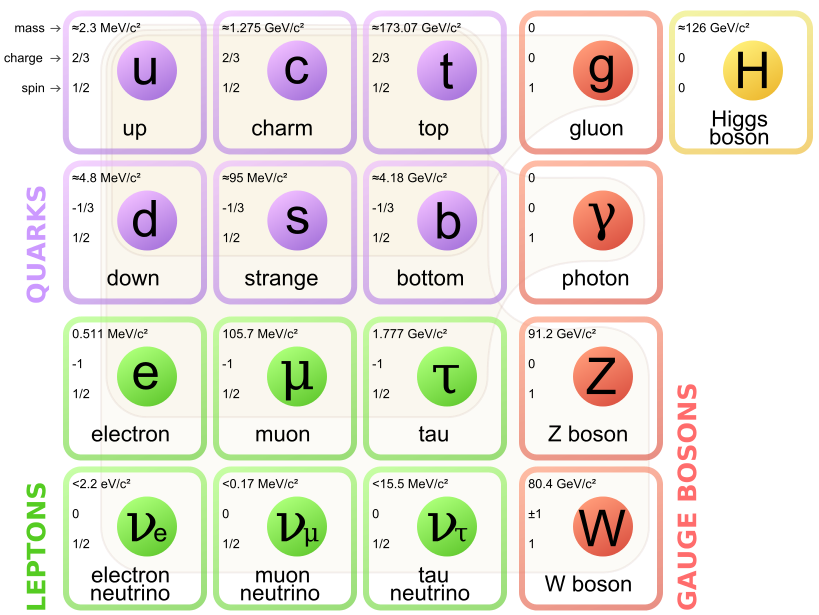
\includegraphics[width=0.85\textwidth]{figures/theory/Standard_Model_of_Elementary_Particles.png}
		\caption{List of standard model elementary particles}
		\label{fig:SM:part}
	\end{center}
\end{figure}

\indent  Interactions in the SM are described by non-abelian Yang-Mills gauge theory with the gauge group $SU(3)_C \times SU(2)_L \times U(1)_Y$ where $SU(3)_C$ corresponds to the strong interaction and $SU(2)_L \times U(1)_Y$ corresponds to the electroweak interactions. 

\indent The quarks can interact via the strong interaction described by the $SU(3)_C$ symmetry.  These quarks carry color charge in addition to their electromagnetic charges.  The gluons mediate the strong interactions but unlike electrically neutral photons, gluons carry color charge.  The self-interaction of the gluon causes the coupling strength of the strong coupling constant $\alpha_s$ to diverge at low energies.  This phenomenon, called confinement, ensures that quarks are confined to be within composite color singlet states in the form of hadrons.  At the same time, the running of $\alpha_s$ approaches zero at high energy; forming a phenomenon known as asymptotic freedom. \\

\indent For energetic particles like those produced in proton-proton collisions at the LHC, colored partons will recursively radiate collinear gluons and quark/anti-quark pairs in a parton shower. These partons eventually form color-singlet hadrons once the energy scale is lower then IR-cutoff scale due to confinement.  The result is a jet of color-neutral baryons and mesons localized in a narrow cone in the direction of the initial colored parton. \\

\indent Both quarks and leptons also interact via the weak interaction.  Specifically, the left handed component of the fermions form an $SU(2)_L$ doublet while the right handed handed components form an $SU(2)_L$ singlet.  Therefore, only the left handed components of SM fermions carry weak charge and interact via the weak interaction.  \\

\indent The generators of the gauge groups correspond to the massless spin one vector bosons.  The $W^\pm$ and $Z$ bosons acquire mass through spontaneous electroweak symmetry breaking using the Higgs mechanism.  This is accomplished using an additional $SU(2)_L$ doublet of complex spin zero fields, the Higgs field.  The Higgs has a nonzero vacuum expectation value (VEV) at the minimum of its quadratic potential shown in equation \ref{eqn:Higgs}.  When $\lambda > 0$ and $m_H^2 < 0 $, $\braket{H} = \sqrt{-m_H^2/2\lambda}$.  \\

\begin{equation}
\label{eqn:Higgs}
V(H) = m_H^2 |H|^2 +\lambda |H|^4
\end{equation}

\indent This breaks the $SU(2)_L \times U(1)_Y$ electroweak symmetry and leaves only the $U(1)_{em}$ electromagnetism invariant.  Meanwhile, the other gauge bosons from $SU(2)_L \times U(1)_Y$ gains a longitudinal degree of freedom from degrees of freedom associated with the Higgs doublet and thereby gaining mass.  The photon, $W^\pm$ and $Z$ bosons are therefore linear combinations of the original $SU(2)_L and U(1)_Y$ generators.  The Higgs boson also gives fermions their mass through Yukawa couplings. \\

\indent After symmetry breaking, only one neutral scalar component of the Higgs doublet is left.  This is the massive Higgs boson observed in July 2012 at the LHC.  \\

\section{Introduction to Super-Symmetry}
\label{Theory:QFT}

%\indent Current combined measurement of the Higgs boson at ATLAS and CMS gives an observed Higgs mass of $125.09\pm0.21$(stat)$\pm0.11$(syst) GeV.\cite{Higgs2016}  Plus $\braket{H} \sim 174 \gev$ due to experimental measurements of the properties of the weak interactions.  This implies that the parameters $\lambda$ and $m_H^2$ in the Higgs potential in equation \ref{eqn:Higgs} have the values of $0.126$ and $-(92.9 \gev)^2$ assuming SM is the correct effective field theory.  \\

\indent Theoretical calculations of the self interaction of the Higgs field give enormous quantum corrections to $m_H^2$.\cite{MartinSUSY}  For example, the correction to $m_H^2$ from a loop containing a Dirac fermion $f$ with mass $m_f$ is given in equation \ref{eqn:Higgs:Loopf}.  The Feynman diagram associated with the fermion loop is shown in figure \ref{fig:Higgs:Loopf} \\

\begin{equation}
\label{eqn:Higgs:Loopf}
\Delta m_H^2 = - \frac{|\lambda_f|^2}{8\pi^2}\Lambda^2_{UV} + ....
\end{equation}

\begin{figure}[htbp]
	\begin{center}
		\includegraphics[width=0.45\textwidth]{figures/theory/loopf.png}
		\includegraphics[width=0.45\textwidth]{figures/theory/loopS.png}
		\caption{One-Loop corrections due to a Dirac fermion $f$ and a scalar $\tilde{f}$ to the Higgs mass parameter $m_H^2$}
		\label{fig:SM:Loopf}
	\end{center}
\end{figure}

\indent $\lambda_f$ is the Yukawa coupling between the fermion and the Higgs and $\Lambda_{UV}$ is the ultraviolet cutoff used to regulate the loop integral.  $\Lambda_{UV}$ can be interpreted as around the energy scale of new physics.  Since the scale of new physics maybe orders of magnitudes larger then the electroweak scale, the quadratic dependence of $m_H^2$ on $\Lambda_{UV}$ makes the Higgs potential extremely sensitive to new physics. This sensitivity to high mass scales for the Higgs potential is referred to as the hierarchy problem.  \\ %Additional terms also exists in the correction but they grow at most logarithmically in $\Lambda_{UV}$. \\

\indent Supersymmetry (SUSY) solves this problem by proposing that there exist a new space-time symmetry with respect to the transformation $Q$ that turns fermions into bosons and bosons into fermions.\\

\begin{equation}
\label{eqn:Higgs:Loopf}
Q\ket{Boson} = \ket{Fermion} ~~~~~~~~~~~~~~~~~~~~~~~~~~~~ Q\ket{Fermion} = \ket{Boson}
\end{equation}

\indent The supersymmetric Lagrangian is invariant under transformations of $Q$ and $Q^{\dagger}$.  In order for this to be satisfied, SUSY proposes the existence of a supersymmetric partner (superpartner) to every known SM particle.  SM particles and their superpartners are related to each other by the Q transformation and differ from each other by spin $1/2$.  If SUSY was an exact symmetry then the SM particle and its superpartner must have the same mass.  However, we have yet to discover even a single superpartner to the SM at collider experiments.  Therefore, SUSY must be broken at low energies and the superpartners have significantly more mass then their SM counter parts.  \\

\indent Supersymmetry breaking can occur in many ways; the details of which are beyond the scope of this thesis.  More details on SUSY symmetry breaking can be found in \cite{MartinSUSY}.  A brief summary of one example of supersymmetry break called Gauge-mediated supersymmetry breaking (GMSB) will be given here.   In GMSB, some scalar fields in the SUSY Lagrangian gains a vacuum expectation value due to their potential energy shape.  This symmetry breaking gives mass to some fermions and their super-partners called messengers.  Both the scalars and the messengers are too heavy to be directly detectable and are not the SM superpartners.  \\

\indent Instead, the messengers contribute effective mass to the superpartners of SM particles via loop interactions.  Gauge symmetry ensures that the loop correction to the SM gauge bosons are zero to all orders of magnitudes, but the same protection is not afforded to their superpartners, the gauginos.  These gauginos gain effective mass through one-loop diagrams involving virtual messenger particles.  In a similar fashion, the scalar partners to SM fermions gain effective mass through two-loop diagrams involving virtual messengers and SM gauge bosons.  In these way, GMSB leads to heavier superpartners relative to their SM counter parts.  \\

%\indent For the purpose of this document, we will only look at the phenomenological consequences of heavy superpartners and not be concerned with the exact SUSY breaking method.  \\

\indent In general, if a complex scalar particle $\tilde{f}$~with mass $m_{\tilde{f}}$~exists and couples to the Higgs according to the term $-\lambda_S|H|^2|\tilde{f}|^2$ then correction to the Higgs mass due to the loop diagram in figure \ref{fig:SM:Loopf} is given in equation \ref{eqn:Higgs:LoopS}. \\

\begin{equation}
\label{eqn:Higgs:LoopS}
\Delta m_H^2 = \frac{\lambda_s}{16\pi^2}[\Lambda^2_{UV} - 2m_{\tilde{f}}^2 \ln{\Lambda_{UV}/m_{\tilde{f}}}+ ....]
\end{equation}

\indent This correction also contains a quadratically divergent term that has an opposite sign to equation \ref{eqn:Higgs:Loopf}.  The two quadratic contributions to $m_H^2$ will cancel if $|\lambda_f|^2 = \lambda_s$ and we are left with only a term that is proportional to $\ln{\Lambda_{UV}/m_{\tilde{f}}}$. In fact, this cancellation of quadratically divergent term will occur not only for the one loop case, but for all orders of magnitude in perturbation theory if supersymmetry exists. \\

\indent The term that remains after cancellation is proportional to equation \ref{eqn:Higgs:logterm}. \\

\begin{equation}
\label{eqn:Higgs:LoopS}
\Delta m_H^2 \sim m_{\tilde{f}}^2[\frac{\lambda_s}{16\pi^2}\ln{\Lambda_{UV}/m_{\tilde{f}}}]
\end{equation}

\indent Its important to note that while the correction is now not so strongly dependent on $\Lambda_{UV}$ because of the natural log, the correction term is also directly proportional to $m_{\tilde{f}}^2$.  This implies that the superpartners masses cannot be too large, otherwise the correction to $m_H^2$ is again too large.  If we set $\Lambda_{UV}$ to approximately the Planck scale $M_P$ and $\lambda_s \sim 1$, we find that $m_{\tilde{f}}$~for the lightest supersymmetric particle should not be heavier then the $\tev$ scale if we want to avoid any unphysical fine-tuning on the Higgs mass.\cite{MartinSUSY}  \\

\indent In particular, we know that the superpartner to the top quark has a coupling to the Higgs of order $1$ due to $\lambda_S = |\lambda_f|^2 \sim 0.94^2$. This makes searches for the stop especially interesting as it is potentially within reach of the energy of the LHC. \\

\subsection{R-Parity Conservation}

\indent Supersymmetry introduces many new interactions not found in the SM.  Some of these interactions directly violate total lepton and baryon numbers.  If such interactions exist then the half-life of a proton may be only a tiny fraction of a second.  However, proton decay experiments have shown that the proton half-life exceeds $10^{32}$ years.  A new discrete symmetry, called R-parity, is introduced to remove these B and L violating terms from the supersymmetric Lagrangian.  \\

\indent The quantity $P_R$ defined in equation \ref{eqn:PR} and must multiply to 1 for all interaction vertexes for R-parity to be conserved. $P_R$ equals $1$ for all SM particles and equals $-1$ for all superpartners.  \\

\begin{equation}
\label{eqn:PR}
P_R = (-1)^{3(B-L)+2s}
\end{equation}

\indent R-parity conservation has several important phenomenological consequences.  In R-parity respecting SUSY, superpartners are always produced in pairs.  Superpartners must always decay into other superpartners forming a long decay chain of SUSY particle to SUSY particle that ultimately end in the lightest supersymmetric particle (LSP) which is absolutely stable.  If the LSP is electrically and color neutral, then it is an attractive dark matter candidate.  \\

\indent In this search, we assume R-parity is conversed and the LSP is a weakly interacting neutralino.  \\

\chapter{General Analysis Strategy}
\label{chap:AnaStrategy}
\section{ R-Parity Conserving SUSY Searches in Regions with Large Mass Splittings }

\indent In R-parity conserving SUSY searches, the sought-after supersymmetric particles are produced in pairs.  Each particle decays via a chain that ends in a stable, lightest super-symmetric particle (LSP).  If the LSP is weakly interacting, it can not be directly detectable by the ATLAS detector and must be inferred from transverse momentum conservation as \MET.  The rest of the products from the decay chain will be a series of SM particles.  ~\\

\indent All searches must distinguish between signal SUSY processes and background SM processes that mimic the signal detector signature.  Most search methods often place a special emphasis on identifying the LSP as this is the one decay product that is unique to SUSY events.  Practically this generally means searching for events with large amount of \MET.  \\

\indent In regions with a large mass splitting between the sparticle and the LSP, the decay of the original sparticle generates large amounts of momentum for the LSP.  Searches targeting high sparticle masses with large mass splittings therefore target the large amount of $\MET$ generated by the LSP as a method to separate signal from background. The $\met$ distributions for stop signals with $(m_{\stop}, m_{\ninoone}) = (1000 \gev,1 \gev)$ and $(600 \gev, 300 \gev)$ are shown in Figure \ref{fig:presel:MET1}. ~\\

\begin{figure}[h!]
%\begin{center}
\centering
    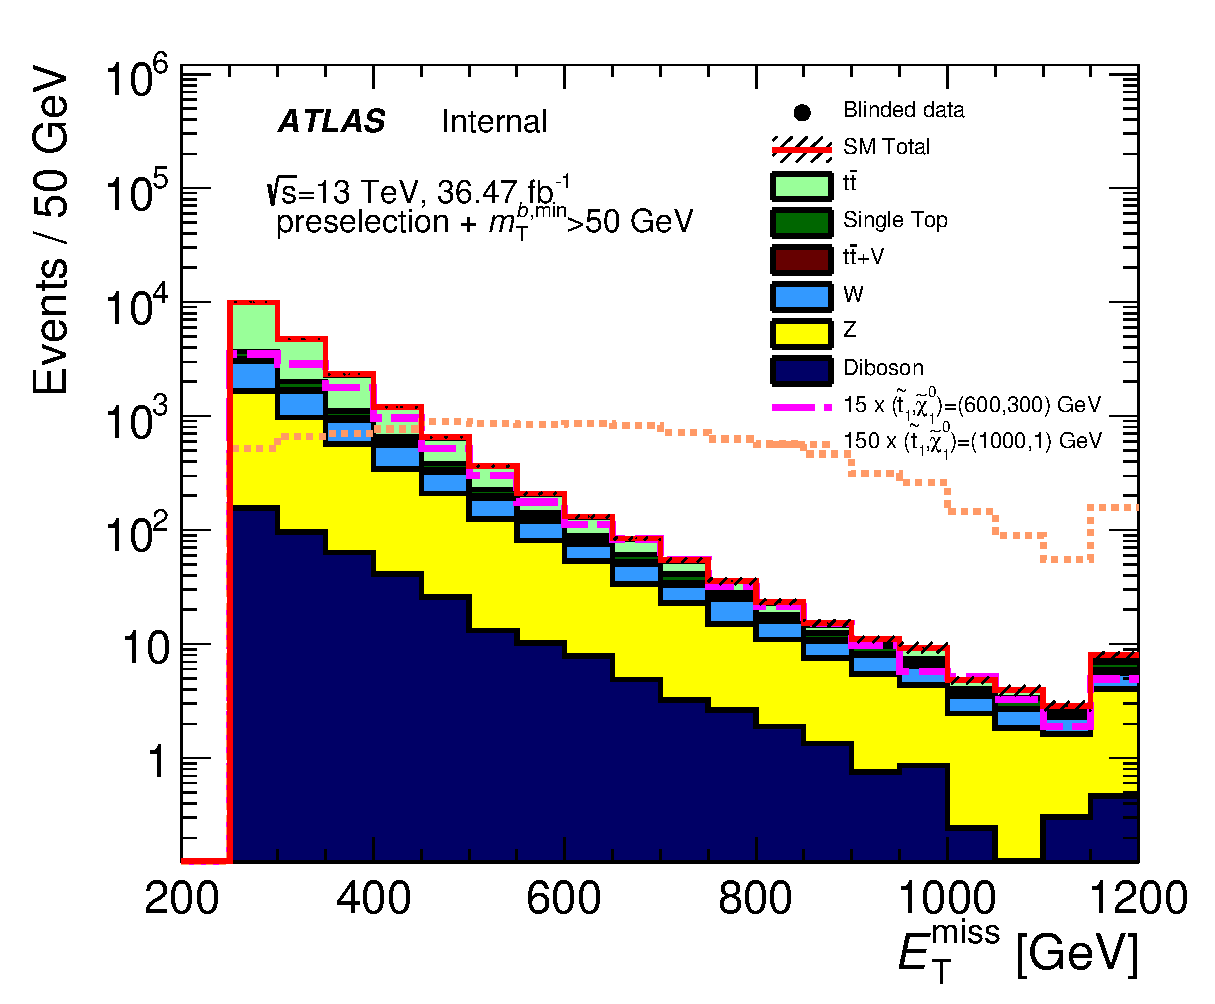
\includegraphics[width=0.85\textwidth]{figures/preselection/Met_preCutSRPlot_withRatio_log.eps}\hspace{0.05\textwidth}
\caption[Stop signal with $m_{\stop}-m_{\ninoone} >> m_t$ and SM background $\met$ distribution after loose preliminary selections for $\met>250 \gev$, zero leptons and at least four jets]{ $\met$ distribution for $(m_{\stop}, m_{\ninoone}) = (1000 \gev,1 \gev)$ and $(600 \gev, 300 \gev)$ stop signal and expected SM background.  The signal cross section has been scaled up by 150 and 15 respectively for better visibility.  Basic selections ensuring well reconstructed $\met$, no leptons, and minimal jet multiplicity requirements are applied.  Details on selections can be found in reference [\cite{stop0LCONF}]. }
\label{fig:presel:MET1}
%\end{center}
\end{figure}

\indent Searches often use other kinematic variables that also depend on $\met$.  Some examples include the $\mtbmax$ and $m_{eff}$ defined in equations \ref{eqn:mtbmax} and \ref{eqn:meff}. \\

\begin{equation}
%\begin{align}
\mtbmax = \sqrt{  (E_{T,b} +\met )^2 - ( \vec{p}_{T,b} + \vec{E}_{T}^{miss} )^2 }
\label{eqn:mtbmax}
%\end{align}
\end{equation}

\begin{equation}
%\begin{align}
m_{eff} =  \met + \sum_{visible~objects} \pt 
\label{eqn:meff}
%\end{align}
\end{equation}

\indent $\mtbmax$ is the transverse mass between $\met$ and the b-jet that is furthest away in $\phi$ from $\met$.  $m_{eff}$ is the scalar sum of all visible objects' $\pt$ plus the $\met$.  While both variables capture additional kinematic information, both are strongly correlated with the total magnitude of $\met$.  The $\mtbmax$ distribution for $(m_{\stop}, m_{\ninoone}) = (1000 \gev,1 \gev)$ and $(600 \gev, 300 \gev)$ stop samples is shown in Figure \ref{fig:stopMtbmin}.  The $m_{eff}$ distribution for gluinos is shown in Figure \ref{fig:gluino_meff}.  SM backgrounds correspond to the solid stacked histograms. \\

\begin{figure}[h!]
  \begin{center}
    \begin{subfigure}[b]{0.30\textwidth}
        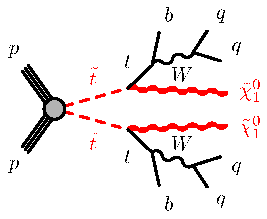
\includegraphics[width=\textwidth]{figures/feynDiag/stst-bqqbqqN1N1-tt.eps}%\hspace{0.05\textwidth}
                \caption{ }
    \end{subfigure}
    \begin{subfigure}[b]{0.45\textwidth}
        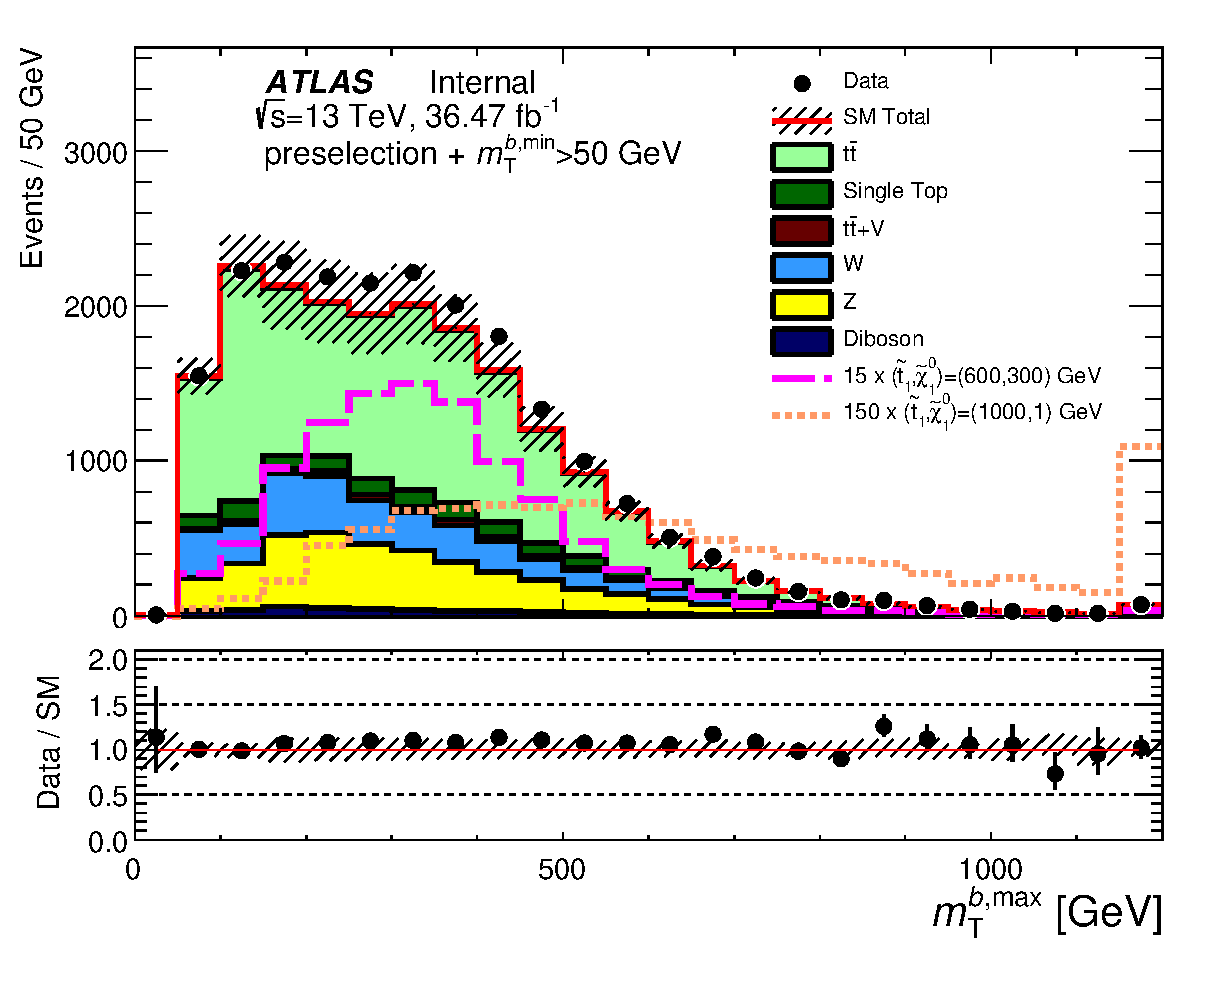
\includegraphics[width=\textwidth]{figures/preselection/MtBMax_preCutSRPlot_withRatio.eps}
                \caption{ }
    \end{subfigure}
\end{center}
\caption[Stop signal with $m_{\stop}-m_{\ninoone} >> m_t$ and SM background $\mtbmax$ distribution after loose preliminary selections for $\met>250 \gev$, zero leptons and at least four jets]{ (a) Feynman diagram for stop production and decay. (b) \mtbmax distribution for $(m_{\stop}, m_{\ninoone}) = (1000 \gev,1 \gev)$ and $(600 \gev, 300 \gev)$ samples after loose selections for $\met>250 \gev$, zero leptons and at least four jets.\cite{stop0LCONF} }
\label{fig:stopMtbmin} 
\end{figure}

\begin{figure}[h!]
  \begin{center}
    \begin{subfigure}[b]{0.30\textwidth}
        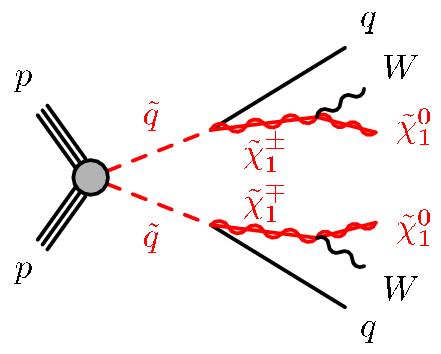
\includegraphics[width=\textwidth]{figures/feynDiag/gluino_onestep.png}%\hspace{0.05\textwidth}
                \caption{ }
    \end{subfigure}
    \begin{subfigure}[b]{0.45\textwidth}
        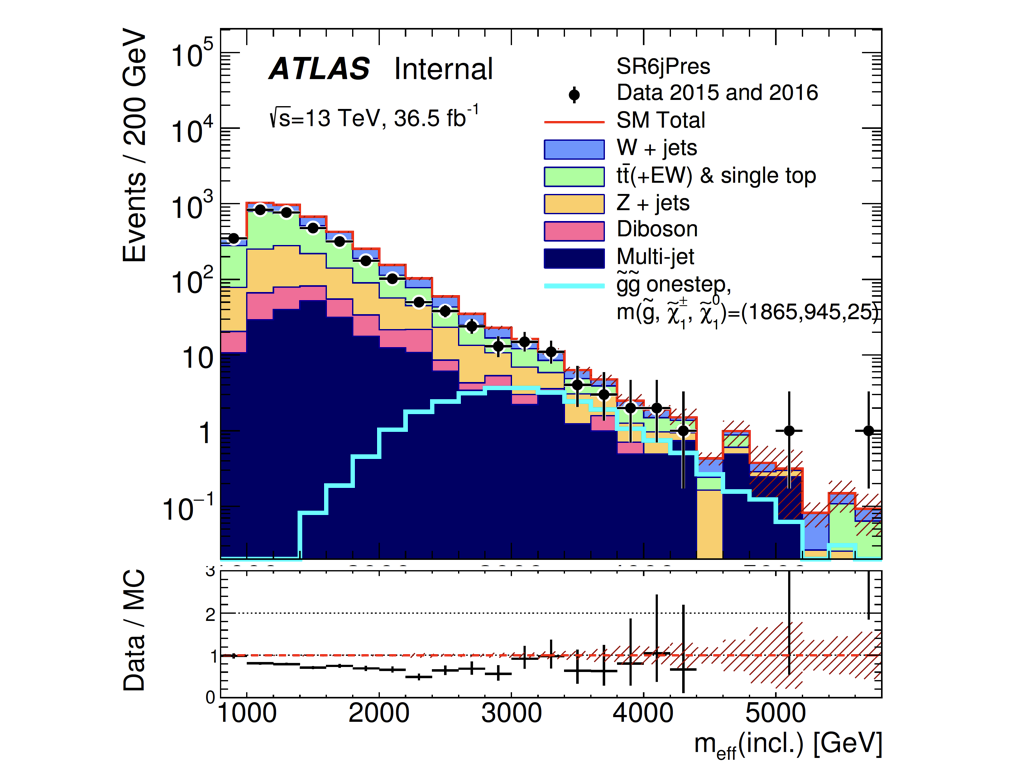
\includegraphics[width=\textwidth]{figures/strategy/gluino_meff.png}
                \caption{ }
    \end{subfigure}
\end{center}
\caption[Gluino signal with large mass splittings and SM background $m_{eff}$ distribution after loose preliminary selections for $\met>250 \gev$, zero leptons and at least six jets]{ (a) Feynman diagram for gluino production and decay. (b) $m_{eff}$ distribution for gluino $(m_{\gluino}, m_{\chinopm}, m_{\ninoone}) = (1865 \gev, 945 \gev, 25 \gev)$ after loose selections for $\met>250 \gev$, zero leptons and at least six jets.\cite{SUSYinclusive0L} }
\label{fig:gluino_meff} 
\end{figure}

\indent Both distributions have large separation power between signal and SM backgrounds.  By making kinematic selections on these sensitive variables, ATLAS and CMS searches are able to gain sensitivity to high sparticle masses with small production cross sections.  For example, current ATLAS and CMS searches can exclude stops to upwards of 1 $\tev$. \\


\section{R-Parity Conserving SUSY Searches in Compressed Regions}


\indent When the mass splitting between the original sparticle and its decay products becomes small, the sparticle has little energy to generate momenta in its decay products.  The result is LSPs with low momenta.  The traditional strategy of searching for events with large amount of $\MET$ therefore fails in this region of parameter space.  This problem is ubiquitous to all regions with small mass splittings.  We refer to all such regions as compressed regions.  ~\\

\indent  In our analysis, the super-partner of the top, the stop, is expected to decay into a neutralino and top.  When the stop mass is close to that of the top mass plus the neutralino mass, both the top and neutralino gain very little momenta from the decay.  The invisible neutralinos in turn generate very little missing transverse energy.  This leaves only the visible tops, which are mimicked by SM $\ttbar$. \\

\indent Search methods that depend on variables that are highly correlated with the total magnitude of $\met$, such as $\mtbmax$ and $m_{eff}$, fail to separate stops from SM $\ttbar$.  This plus the fact that the $\ttbar$ production cross section is $50-300\times$ the production cross section of stops for stop masses between 250 and 400 $\gev$ means these search methods have little sensitivity to the compressed parameter space.  \\ %A High-Luminosity LHC study projects a 2$\sigma$ exclusion limit up to a stop mass of 500 $\gev$ with 300 $\ifb$ of data in this region.\cite{HLLHC_stop} The projected p-value as a function of stop mass for 300 and 3000 $\ifb$ of data is given in Figure \ref{fig:HL_LHC:p_value} \\

%\begin{figure}[h!]
%  \centering
%	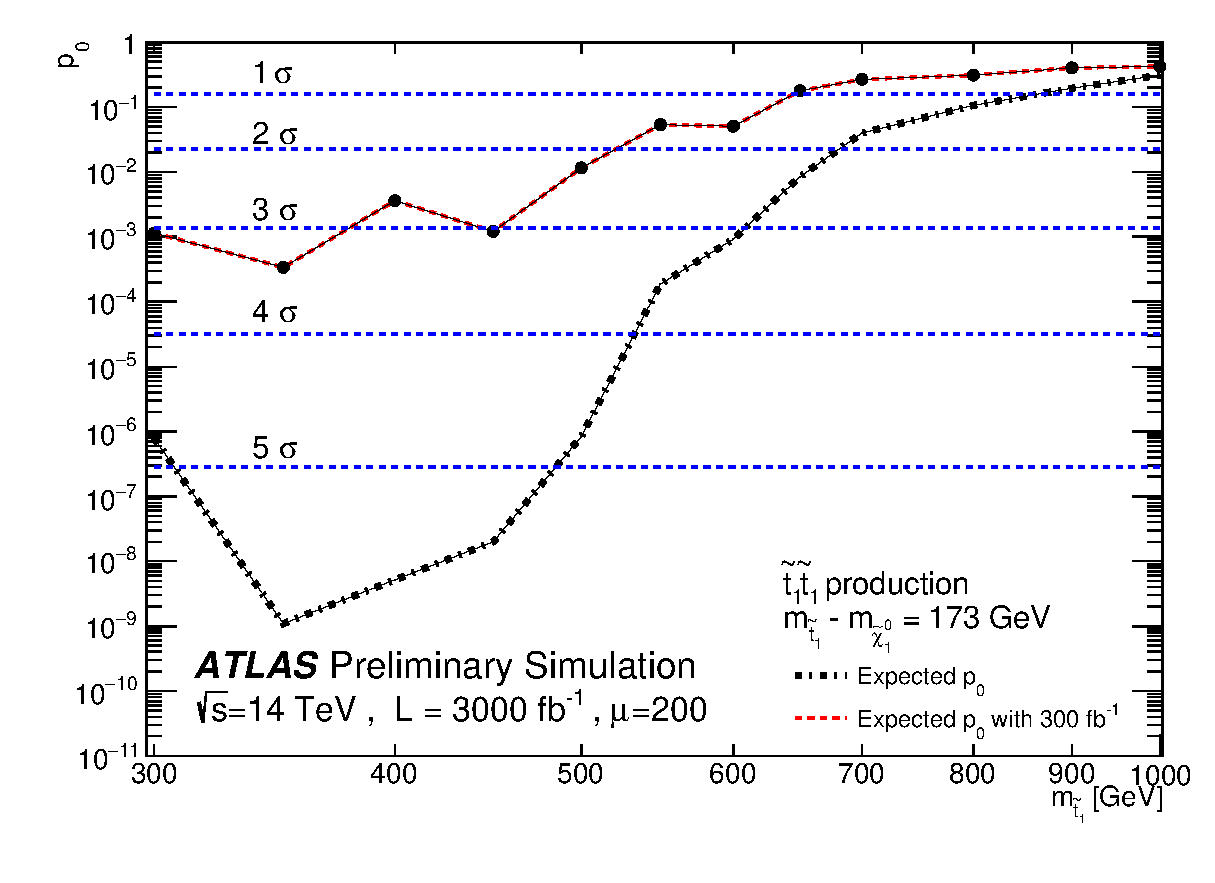
\includegraphics[width=0.65\textwidth]{./figures/strategy/HLLHC_pvalue.eps}
%\caption{Projected HL-LHC sensitivity to the $\Delta m = m_t$ region with 300 and 3000 $\ifb$ of data.  Sensitivity is quantified in terms of the p-value $p_0$.  2 sigma exclusion is reached for stop masses below 500 $\gev$ with 300 $\ifb$. Figure taken from \cite{HLLHC_stop }}
%\label{fig:HL_LHC:p_value}
%\end{figure}

\indent However, the soft decay products can gain additional momenta if the entire system is boosted by hard initial state radiation (ISR).  The goal of the traditional searches has always been to identify the presence of the LSPs and use their presence to distinguish between signal and background.  Instead of targeting events with large amount of $\MET$, we use the correlations between the LSP momenta and any ISR jets to identify LSPs in compressed regions.\cite{Pheno1,Pheno2}  Because LSPs gain little momenta from stop decays, the correlation between ISR and LSPs in compressed regions tend to be extremely strong.  By targeting the correlations between ISR and $\met$ instead of the total magnitude of $\met$, we effectively turn a weakness of the compressed region into a strength. \\

\indent For the $p p \rightarrow \antibar{\stop} \rightarrow t\ninoone\tbar\ninoone$ process, the relationship is given by equation \ref{eqn:theory_MET_ISR}. This ratio between the invisible decay products and the total ISR $\pt$ is called \RISR. \\

%\begin{equation}
\begin{align}
\MET \equiv p_{\ninoone\ninoone,~T}^{~\mathrm{lab}} \sim \gamma_{\stop\stop}^{~\mathrm{lab}} \beta_{\stop\stop}^{~\mathrm{lab}} E_{\ninoone\ninoone}^{~\stop\stop} 
\sim \frac{\PTISR}{m_{\stop\stop}} 2\gamma_{\stop}^{\stop\stop} m_{\tilde{\chi}} \sim
\PTISR \frac{ 2\gamma_{\stop}^{\stop\stop} m_{\tilde{\chi}} }{ 2\gamma_{\stop}^{\stop\stop} m_{\stop} } \sim
\PTISR \frac{m_{\ninoone}}{m_{\stop}}\implies\\
\RISR \equiv \frac{\MET}{\PTISR} \sim \frac{m_{\ninoone}}{m_{\stop}}~,\quad\quad\quad\quad\quad\quad\quad\quad\quad\quad\quad\quad
\label{eqn:theory_MET_ISR}
\end{align}
%\end{equation}

\indent The ratio between $\MET$ and ISR $\pt$ is proportional to the ratio between the mass of the LSP and the original sparticle.  It is interesting to note that the back-to-back boost between the two original stops does not affect the correlation between the observable $\MET$ and ISR $\pt$.  Although the LSPs can individually gain momenta from the sparticles boosting against one another, the back-to-back momenta will exactly cancel resulting in zero measurable $\MET$.  \\

\indent The di-LSP system only gains $\pt$ by inheriting it from the boost by the ISR system on the two sparticles.  The fraction of the momenta that is inherited by the di-LSP system is exactly $\frac{m_{LSP}}{m_{sparticle}}$ if the sparticle decay gives no additional momentum to the LSP.  \\

\indent Figure \ref{fig:stop_400_227_ISR_MET_truth} shows the distribution of the $\RISR$ ratio in $p p \rightarrow \antibar{\stop} \rightarrow t\ninoone\tbar\ninoone$ simulation for two different stop masses (350 and 550 $\gev$).   In both cases, the $\Delta m = m_{\stop} - m_{\ninoone}$ is $173 \gev$, only 500 $\mev$ from the $m_t = 172.5$ $\gev$.  Both stop samples sharply peak at exactly $m_{\ninoone}/m_{\stop}$ just as equation \ref{eqn:theory_MET_ISR} predicted.  The gaussian width of each peak has a width of only $\sim4$\%.  No detector resolution effects were included in the simulation and only the all hadronic decay channel was considered. \\

\begin{figure}[h!]
  \centering
	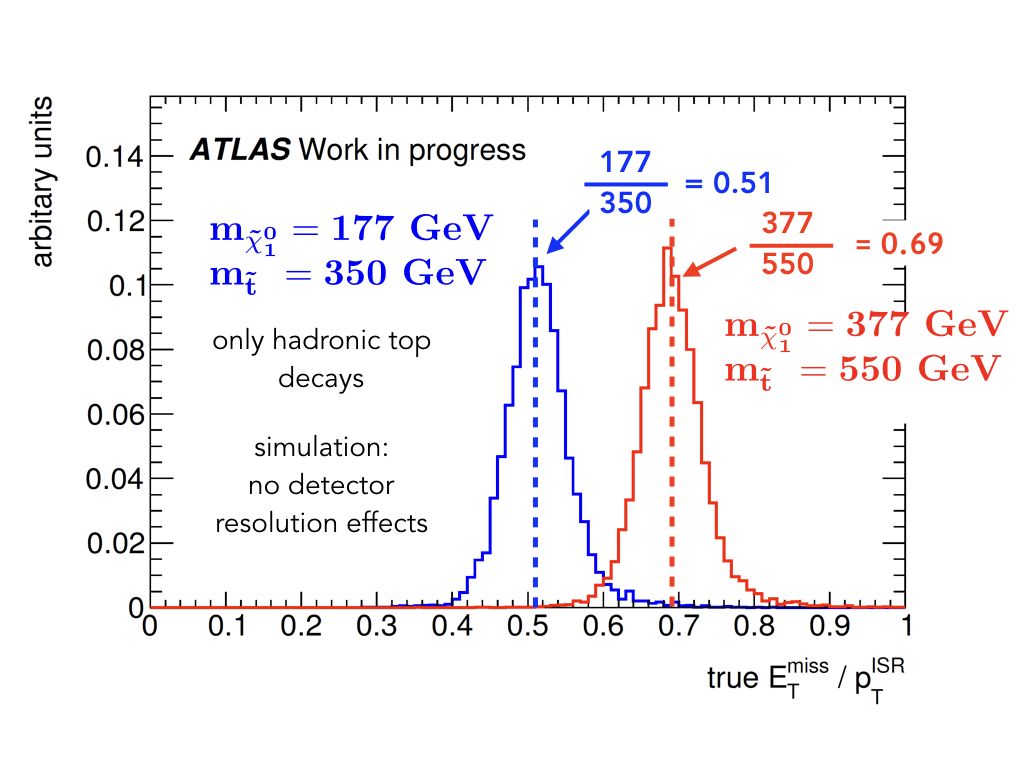
\includegraphics[width=0.65\textwidth]{./figures/strategy/RISR_truth.png}
\caption[$\RISR = \met/\PTISR$ distributions for stop signals with $m_{\stop} - m_{\ninoone} \sim m_t$ in MC simulation]{The $\RISR = \met/\PTISR $ distribution for two different stop samples both with $m_{\stop} - m_{\ninoone} \sim m_t$.  Both stop MC samples peak sharply at $m_{\ninoone}/m_{\stop}$ with only a gaussian width of 4\%.  Deviation from the preferred ratio is limited by the top width, as the top must be pulled off shell to generate phase space. No detector resolution effects where included and only the all hadronic decay channel was considered.}
\label{fig:stop_400_227_ISR_MET_truth}
\end{figure}

\indent The ISR and $\met$ correlations also exist in direction.  ISR and $\met$ are necessarily back-to-back, because the neutralinos recoil in the opposite direction as the ISR.  \\%In comparison, the neutrino gains significant momentum directly from the top decay in $\ttbar$ background and their correlation with ISR is not as absolute.  \\

\indent The relationship between the decay products and ISR also has an additional benefit of being model independent.  This correlation is dictated solely by relativistic kinematics rather than the underlying QFT of any particular model.  The decay products' momentum and direction are determined mostly by two things: how heavy the decay products are and how hard they are kicked by the ISR.  \\

\indent We identify ISR by finding the axis of maximum back-to-back $\pt$, called the thrust axis.  The thrust axis should mimic the axis of back-to-back boost between the ISR and sparticle systems because the back-to-back boost between the ISR and sparticle systems represents the single largest back-to-back kick in events with hard ISR. \\

\indent A schematic representation of the roles of the thrust axis in stop+hard ISR events can be seen in Figure \ref{fig:ISR:ttbar_sig_example}. \\

\begin{figure}[h!]
  \centering
	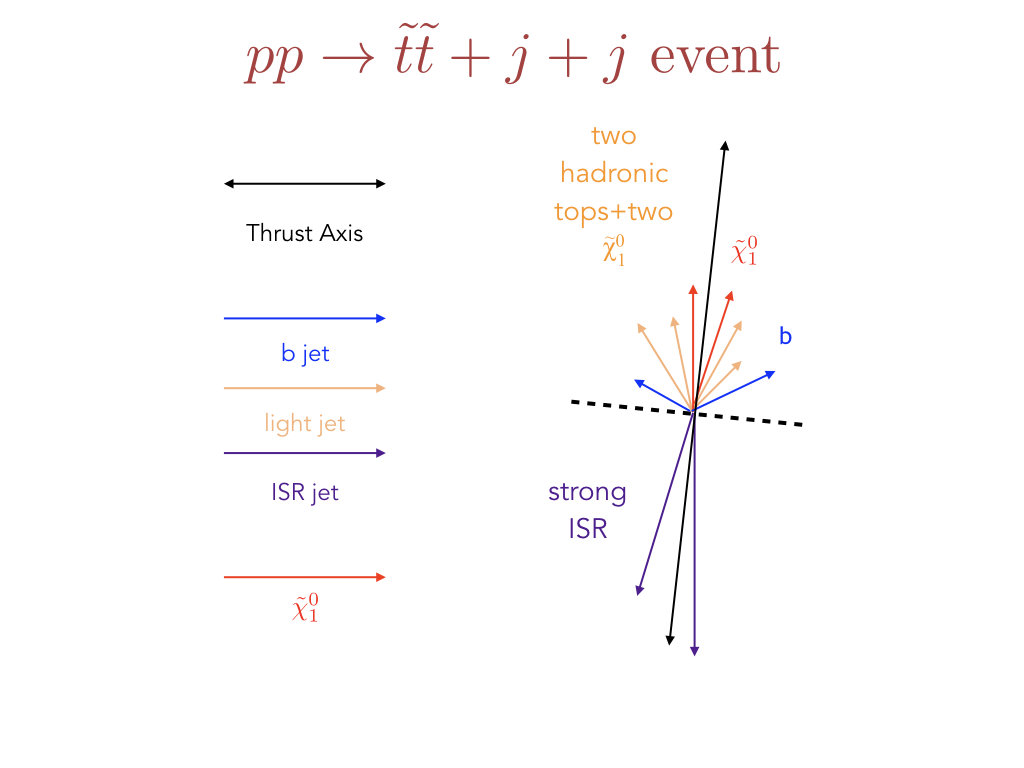
\includegraphics[width=0.85\textwidth]{./figures/strategy/ISR_signal.png}
	\caption[Schematic depictions of stop+hard ISR event kinematics]{Schematic depictions of stop+hard ISR event kinematics.  The thrust axis approximates the direction of back-to-back boost between ISR and stop decay products.  The hemisphere containing $\met$ also contains most of the other stop decay products.  The hemisphere opposite the $\met$ contains the energetic ISR jets. }
	\label{fig:ISR:ttbar_sig_example}
\end{figure}

\indent We divide the event into two hemispheres according to the thrust axis.  The hemisphere with $\met$, called the sparticle hemisphere, is expected to contain mostly stop decay products. The hemisphere opposite the $\met$ should contain the energetic ISR jets.  The accurate ISR identification algorithm preserves the sharp correlations between ISR and $\met$.  \\

\indent Other kinematic properties of the two hemispheres can also be used to separate signal from background.  For example, the number of jets in the sparticle system $\NjV$ and the total transverse mass $\MS$ of the sparticle hemisphere are both expected to be larger in signal.  The $\NjV$ and $\MS$ distributions for signal and SM backgrounds are shown in Figure \ref{fig:presel:jet_MS}. \\

\begin{figure}[h]
  \begin{center}
    \begin{subfigure}[b]{0.40\textwidth}
        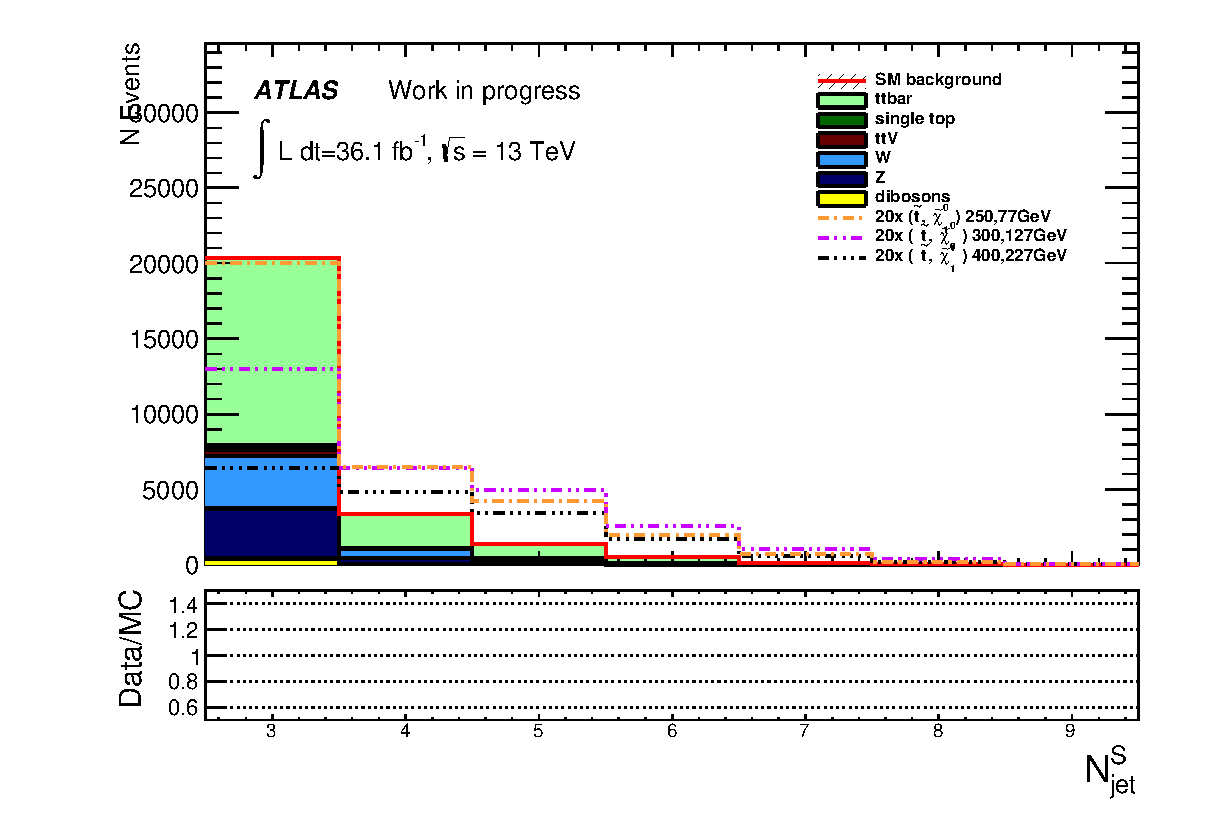
\includegraphics[width=\textwidth]{figures/plotSR/SR_ND1_NjV_0SR.eps}%\hspace{0.05\textwidth}
        \caption{ }
    \end{subfigure}
    \begin{subfigure}[b]{0.40\textwidth}
        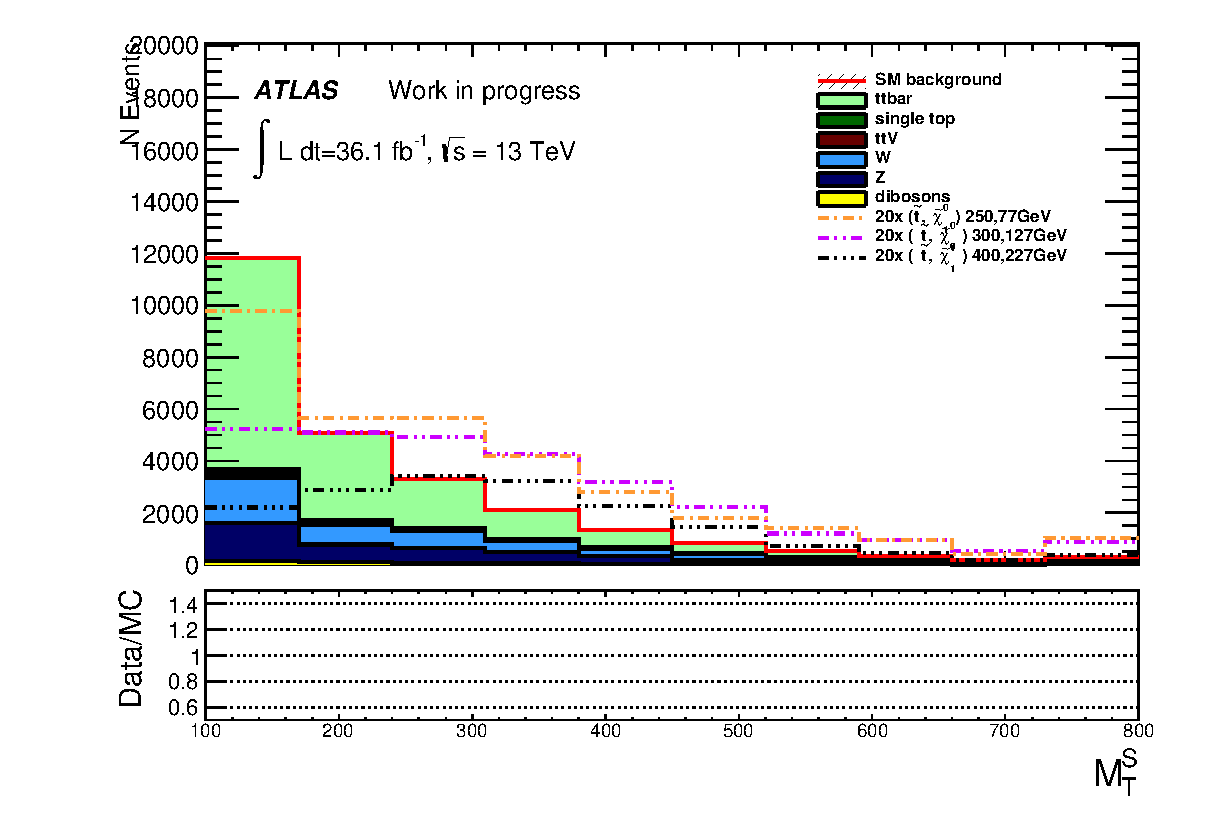
\includegraphics[width=\textwidth]{figures/plotSR/SR_ND1_MS_0SR.eps}%\hspace{0.05\textwidth}
                \caption{ }
    \end{subfigure}
\caption[$\NjV$ and $\MS$ distributions for stop signal and SM background after lose selections for $\met>250 \gev$, zero leptons and at least four jets]{ (a) $\NjV$ distribution for stop signal and SM background after loose selections for $\met>250 \gev$, zero leptons and at least 4 jets.  (b) $\MS$ distribution for stop signal and SM background after loose selections for $\met>250 \gev$, zero leptons and at least four jets. Details on preliminary selections can be found in chapter \ref{chap:Selection_EventPreselection} }
\label{fig:presel:jet_MS} 
\end{center}
\end{figure}

\indent In the stop signal, the six partons from the two top decays are also boosted by the ISR and tend to go in the same direction as the two neutralinos.  In comparison, the dominant $\ttbar$ background tends to have the top and anti-top recoil against one another in a back-to-back fashion.  Therefore, only one set of top decay products are in the same hemisphere at the $\met$.  The result is the signal tends to have higher jet multiplicities and total energy in the hemisphere containing $\met$.  Figure \ref{fig:ISR:ttbarb2b_sig} illustrates this difference between signal and $\ttbar$ background kinematics.  \\

\begin{figure}[h!]
  \centering
	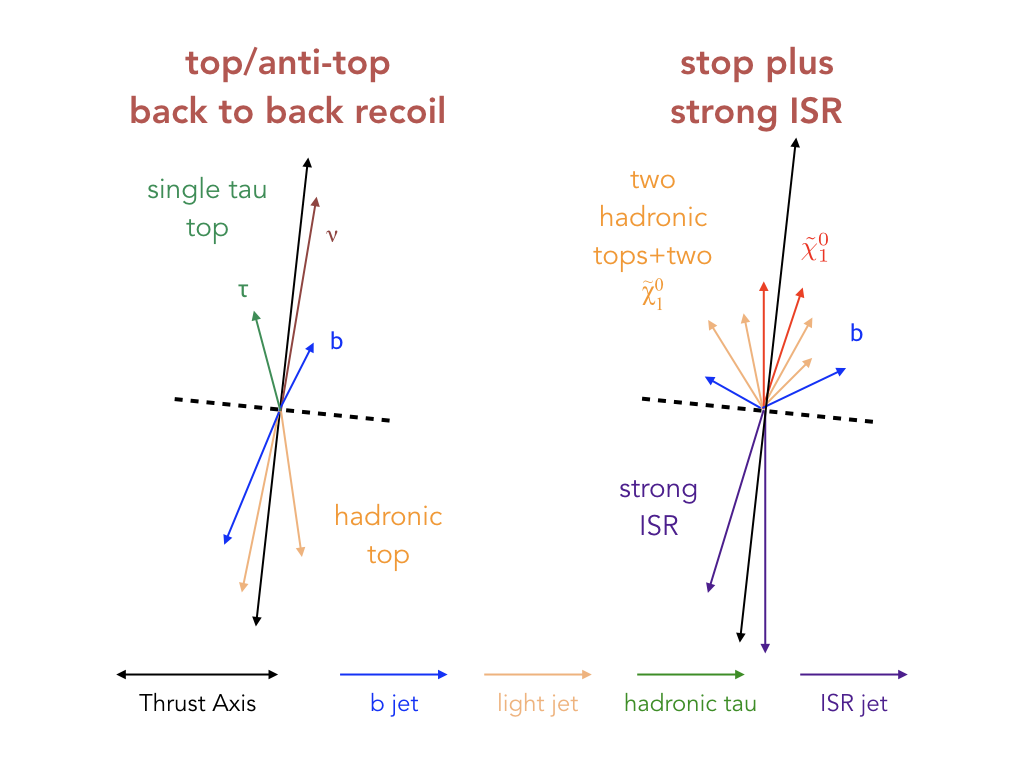
\includegraphics[width=0.85\textwidth]{./figures/strategy/ttbarb2b_stop.png}
	\caption[Schematic depictions of the kinematics of a $\ttbar$ event with the top recoiling against the anti-top in a back-to-back manner and a stop+hard ISR event]{Schematic depictions of the kinematics of a $\ttbar$ event with the top recoiling against the anti-top in a back-to-back manner and a stop+hard ISR event.  The thrust axis approximates the direction of back-to-back boost between ISR and stop decay products in signal and the back-to-back boost between the top and anti-top in the $\ttbar$ background.  This leads to the hemisphere containing $\met$ has greater jet multiplicity $\NjV$ and total transverse mass $\MS$ in signal. }
	\label{fig:ISR:ttbarb2b_sig}
\end{figure}

\indent Chapter \ref{chap:jigsaw} defines the kinematic variables on the sparticle and ISR hemispheres and explains the ISR identification algorithm in greater detail. \\

\indent Selections are made on these sensitive variables forming a signal region (SR) that is optimized to maximize signal sensitivity.  The expected background rates in the signal region are predicted using a combination of MC and data driven techniques.  One common technique involves making kinematically similar control regions (CR) and validation regions (VR). All expected background rates in the signal region have been normalized to control regions defined in chapter \ref{chap:backgrounds}.  The control regions are designed to mimic the background kinematics in the signal region but are orthogonal to the signal region and have low expected signal rate.  We directly measure the background rate using data in the control regions and use simulation to extrapolate background predictions from the control region to the signal region. The validation regions are even closer in kinematic selections to the signal and form an independent cross check on the extrapolation between the control and signal regions. \\

\indent The relationship between control, validation, and signal regions is graphically depicted in Figure \ref{fig:CR_VR_SR_stat1}.  Details on signal region selections can be found in chapter \ref{chap:SignalRegion}.  Details on background estimation, control regions and validation regions can be found in chapter \ref{chap:backgrounds}. \\

\begin{figure}[h!]
  \centering
	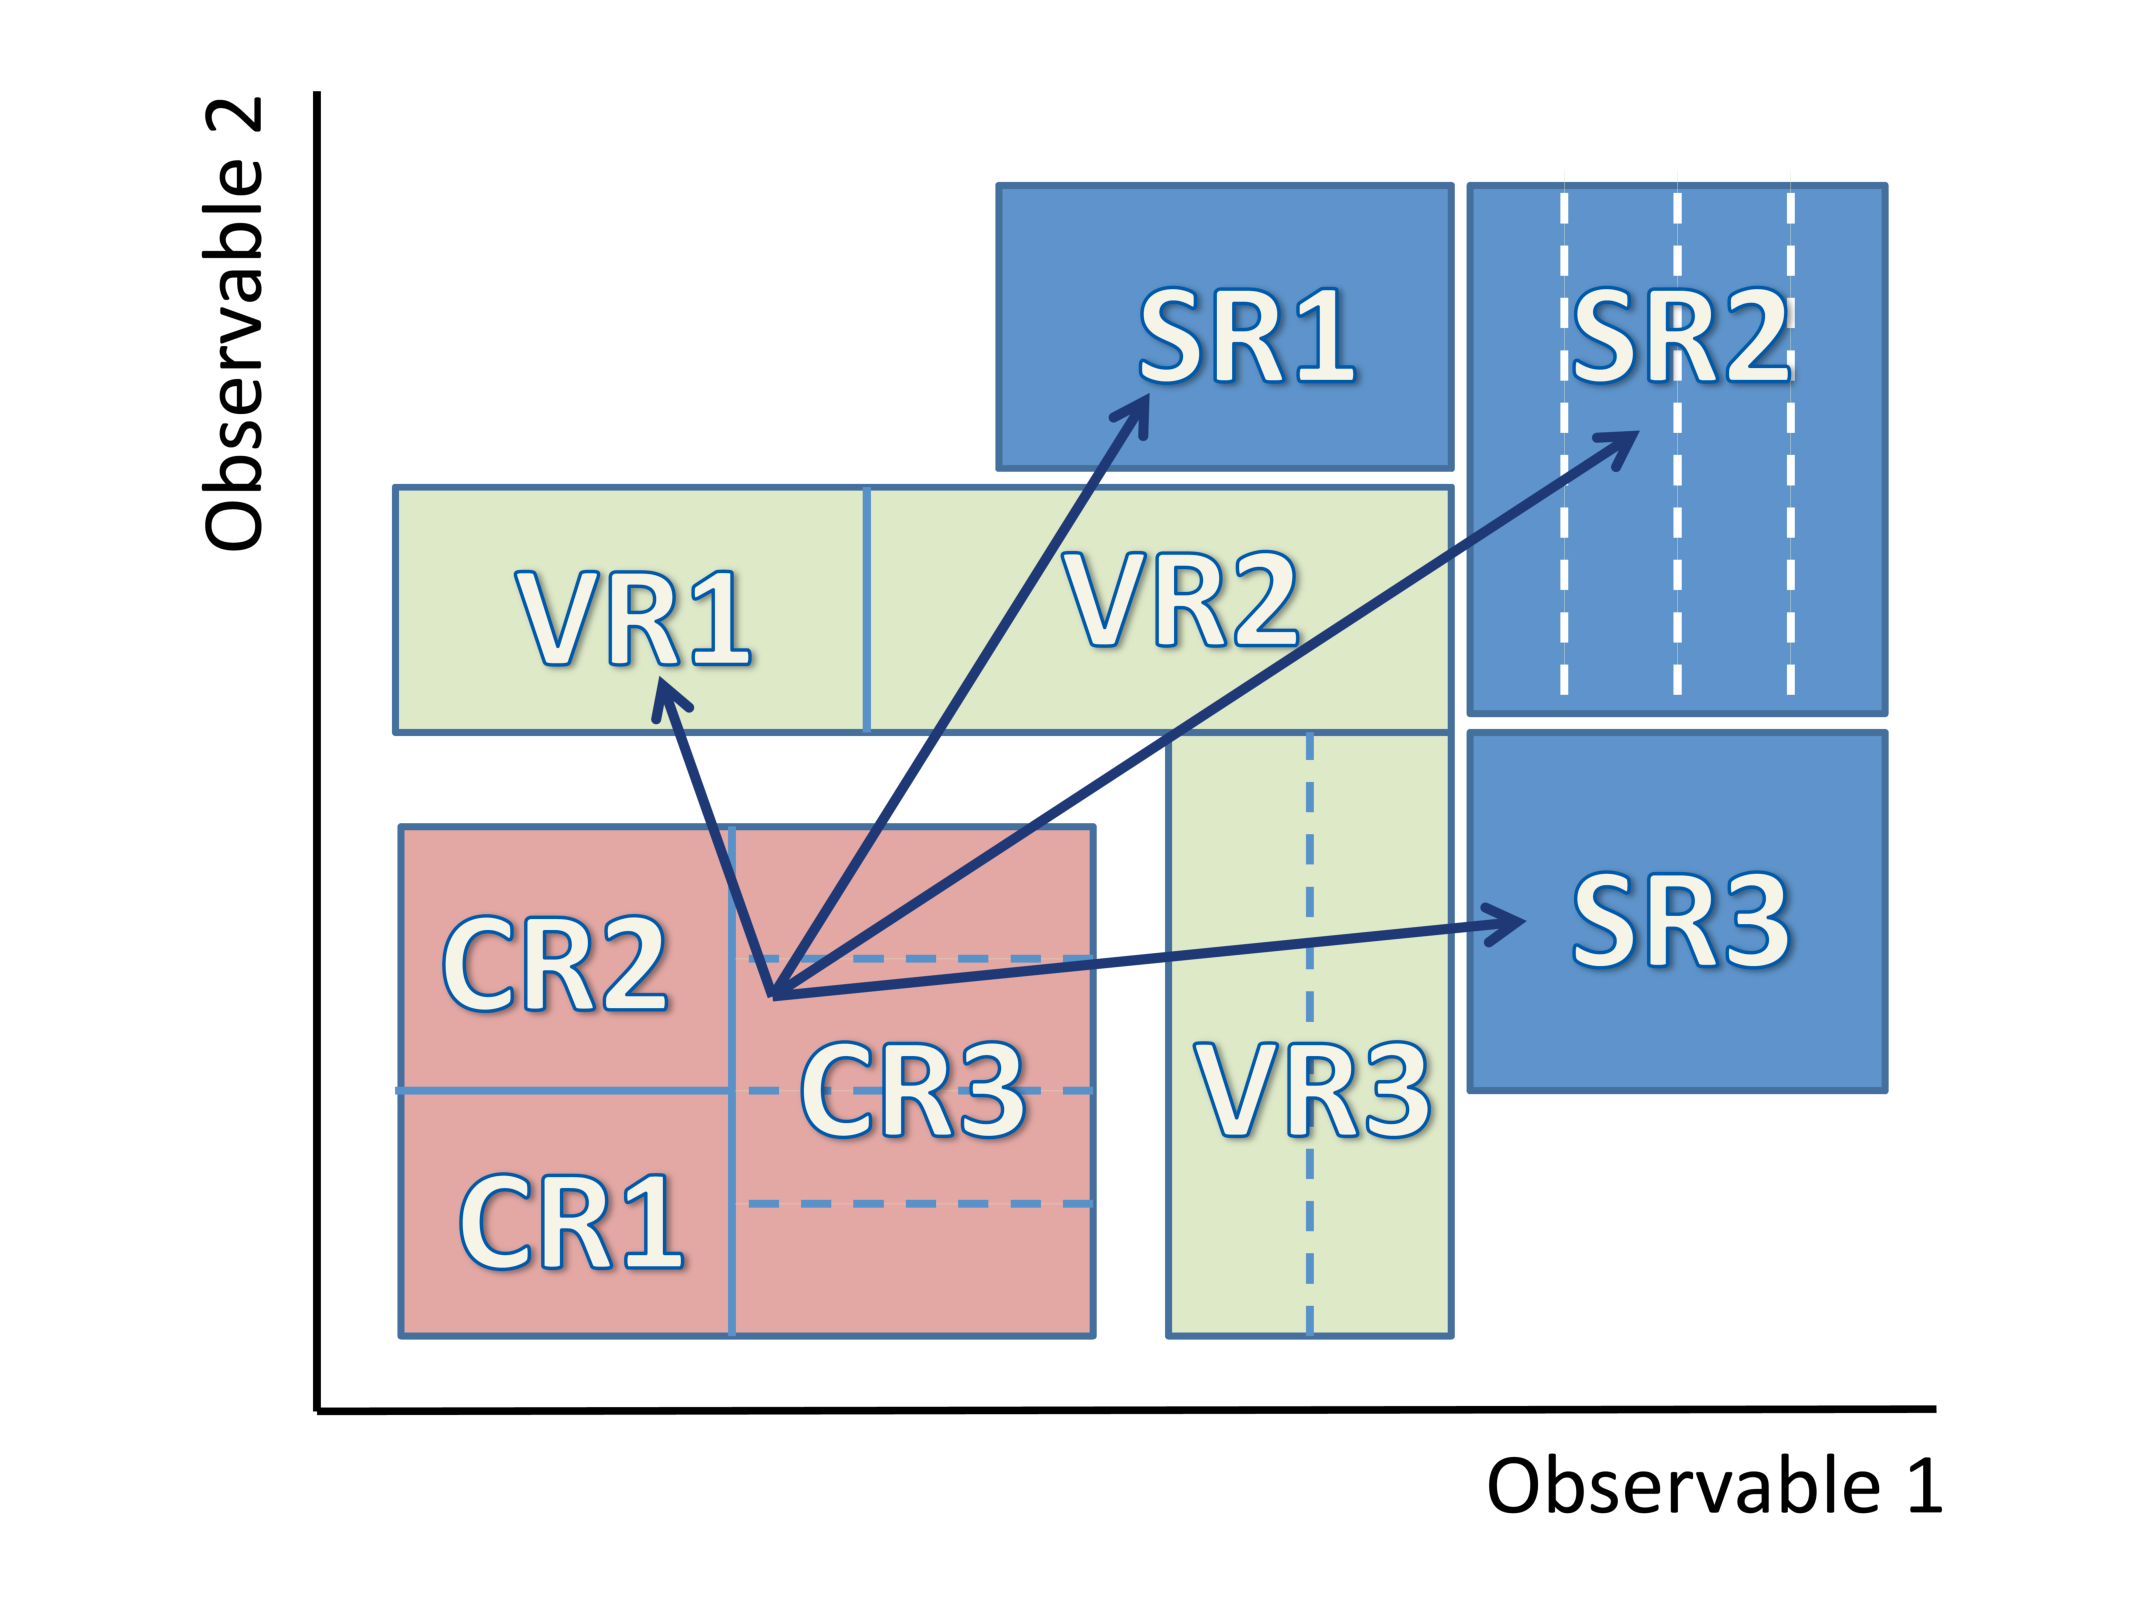
\includegraphics[width=0.65\textwidth]{./figures/statistics/CR_VR_SR.pdf}
\caption[Schematic diagram demonstrating the use of control regions to estimate background rates in the signal region]{Schematic diagram demonstrating the use of control regions (CR) to estimate background rates in the signal region (SR).  Control regions are dominated by background and have few expected signal events.  We can estimate the amount of background we expect in the signal region by measuring the amount of background in the control region and extrapolating to the signal region using MC predictions. Validation regions exist between control regions and signal regions and serve as an independent region to validate background predictions.  }
\label{fig:CR_VR_SR_stat1}
\end{figure}

\indent The data in the signal region is originally blinded to avoid any bias for or against discovery.  We unblind the signal region only after we decide the background prediction in the signal region is well understood based on observations in the control regions and validation regions. \\

%awkward sentence
\indent If an excess of data is found in the signal region after unblinding then a simultaneous fit to all the control regions and the signal region is performed to calculate the statistical significance of any potential excess.   If no excess is found, then a simultaneous fit to all the control regions and the signal region is also performed to quantify the smallest signal cross section that can be excluded.  \\

\chapter{Experimental Apparatus}
\label{chap:Exp}

\indent The study of standard model (SM) physics at the TeV scale and search for potentially new physics beyond the standard model (BSM) is one of the highlights of current physics programs at the Large Hadron Collider (LHC).  The LHC is a circular superconducting particle accelerator capable of accelerating and colliding both protons and lead ions.  The LHC is built in the 27km LEP tunnel between 45 to 170m underground near the city of Geneva.  The entire LHC accelerator complex, shown in Figure \ref{LHC:fig:LHCComplex} is operated by the Organization for European Nuclear Research or CERN. More details on the LHC machine and the CERN accelerator complex can be found in reference [\cite{LHC}]. \\

\begin{figure}[h!]
%\begin{center}
\centering
\includegraphics[width=0.95\textwidth, angle=0]{figures/LHC_ATLAS/AccComplex0700829.pdf}
\caption{ The Large Hadron Collider complex.\cite{LHC} \label{LHC:fig:LHCComplex}}
%\end{center}
\end{figure}

\indent During 2015 to 2016, the LHC collided protons with a center of mass energy of $13$ TeV.  During 2016, the LHC surpassed its design by reaching peak instantaneous luminosities of $1.34 \times 10^{34}$ cm$^{-2}$ sec$^{-1}$.  \\

\indent The LHC uses four major particle detectors located at four interaction points at different locations in the ring to study the result of these collisions.  Two of these, ATLAS and CMS, are hermetic  $4\pi$ general-purpose detectors that study a wide variety of SM and BSM physics including SUSY.   ATLAS and CMS are located at the opposite ends of the ring to ensure equal integrated luminosity.  The two detectors are sensitive to the same physics processes and serve as validations to one another.  The ALICE detector specializes in the collision of heavy ions and LHCb specializes in physics involving the bottom quark. \\

\indent In addition to the 4 major particle detectors, three smaller experiments, TOTEM, MoEDAL and LHCf, study proton-proton scattering cross sections, diffractive processes, and cosmic ray physics.  ~\\

\indent This analysis uses data collected by the ATLAS detector in 2015 and 2016.  A summary of the ATLAS detector is given in section \ref{LHC:detector}. \\

%\section{The CERN Accelerator Complex and the Large Hadron Collider}

%\indent Before collision in one of the LHC experiments, protons are first accelerated through a series of accelerators that form the CERN accelerator complex shown in Figure \ref{LHC:fig:LHCComplex}.  Hydrogen atoms are ionized and the resulting protons are first accelerated to $50 \mev$ by the Linear Accelerator 2 (LINAC2).  Then the protons are injected into a series of circular accelerators, the Proton Synchrotron Booster (PSB), the Proton Synchrotron (PS) and Super Proton Synchrotron (SPS) that further increases the proton energy to 1.4, 25 and 450 GeV respectively.  The protons are arranged into bunches composed of approximately $1.1 \times 10^{11}$ protons each and injected into the LHC.  During 2015 and 2016, the LHC operated with both 50 ns and 25 bunch spacings and can nominally accommodate up to 2808 bunches in a single run. \\

%\begin{figure}[h!]
%\begin{center}
%\centering
%\includegraphics[width=0.65\textwidth, angle=0]{figures/LHC_ATLAS/AccComplex0700829.pdf}
%\caption{ The Large Hadron Collider complex. (Taken from \cite{LHC}) \label{LHC:fig:LHCComplex}}
%\end{center}
%\end{figure}

%\indent The LHC shares the same geometry as LEP with eight arc and eight straight sections.  The main LHC body consist of 1232 dipole Niobium Titanium superconducting magnets that are used to generate the 8.33 Tesla magnetic field necessary to bend the 7 TeV proton beams.  The LHC uses a {\tt two-in-one} magnet design shown in figure \ref{LHC_Xsec} both as a cost saving measure and because of the limited space in the tunnels. The two-in-one magnet design uses a single cryogenic system and vacuum vessel for both proton beams.  \\

%\begin{figure}[h!]
%\begin{center}
%\centering
%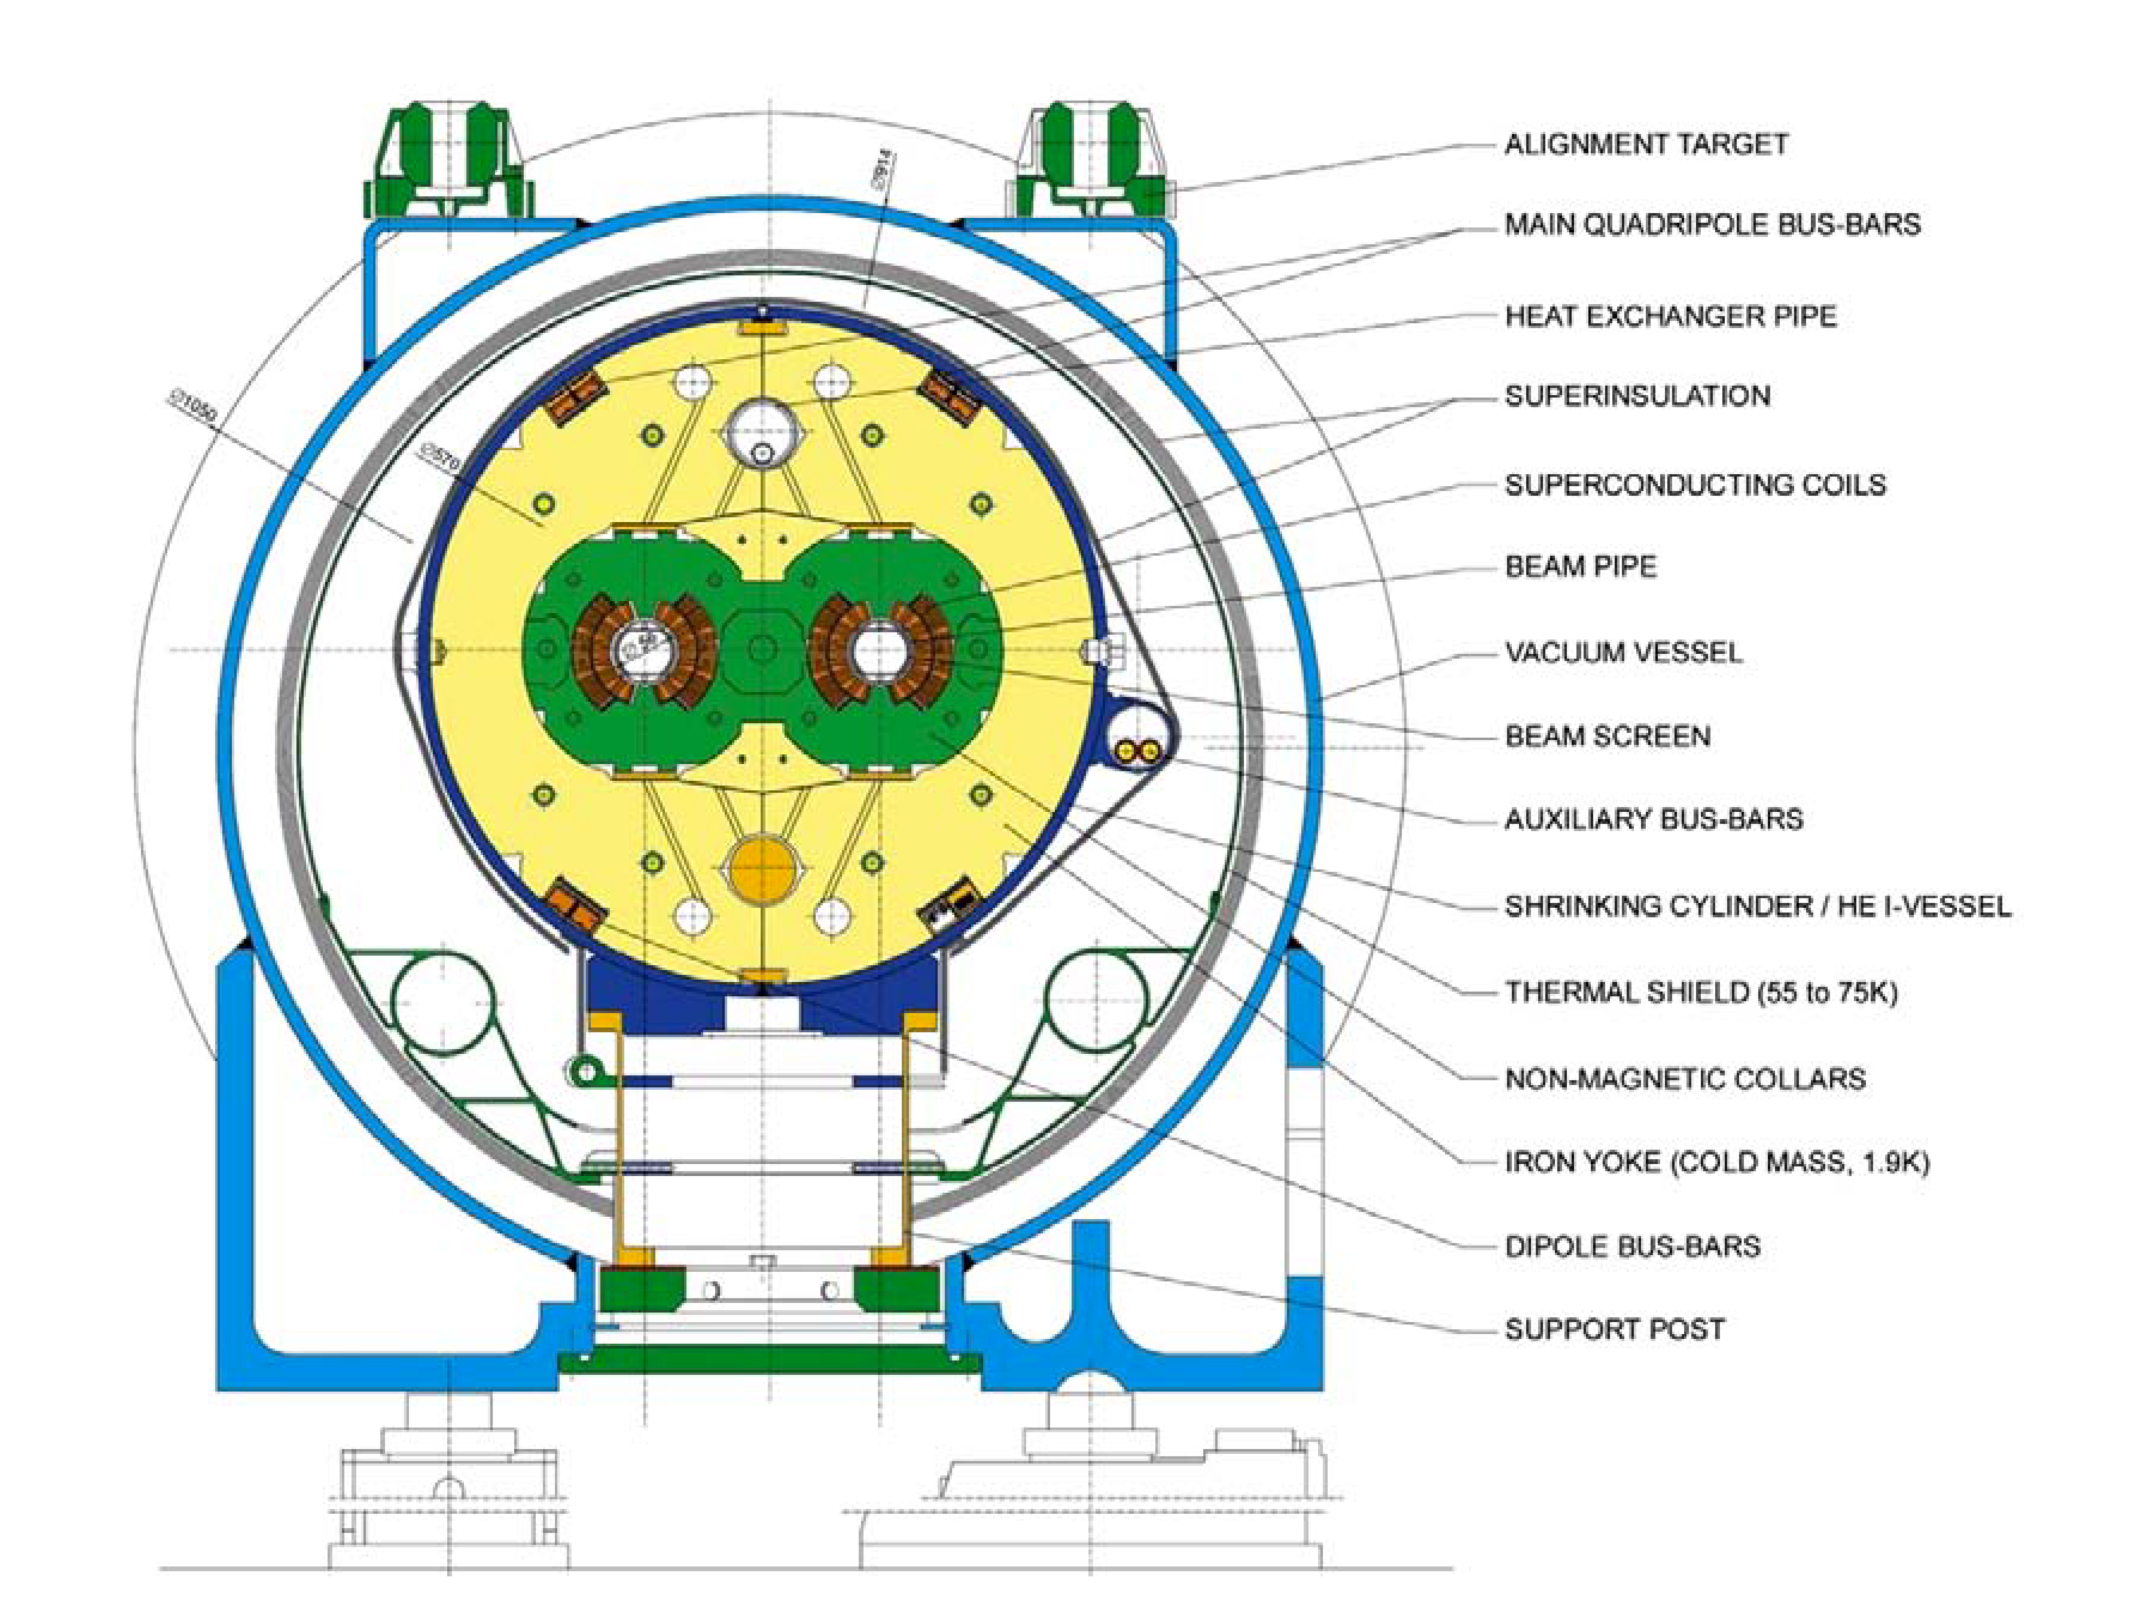
\includegraphics[width=0.75\textwidth]{figures/LHC_ATLAS/LHCCrossSection.pdf}
%\caption{ Cross-Sectional View of a Large Hadron Collider Dipole Magnet.\cite{LHC} }
%\label{LHC_Xsec}
%\end{center}
%\end{figure}

%\indent  392 quadruple magnets are placed after approximately every three dipole sections to stabilize and focus the beam using the principle of strong focusing.  Higher order sextupoles and octupoles magnets provide further corrections. \\

%\indent The beams are accelerated using a 400 MHz superconducting radio frequency (RF) cavity system.  Two independent RF systems are used for the two beams heading in opposite directions.  Each RF system consists of eight cavities.  The total accelerating field inside the cavity is 5 MV/m and each cavity delivers 2 MV of accelerating voltage.  The beams are bent back to repeatedly receive acceleration via the same cavity.  \\

%\indent Further upgrades planed in the Phase 1 shutdown between 2019 and 2021 are projected to further double the instantaneous luminosity and allow the LHC to reach its designed center of mass collision energy of $\sqrt{14} \tev$. \cite{Phase1} \\

\section{The ATLAS Detector}
\label{LHC:detector}

\indent The ATLAS Detector is a general purpose detector designed to search for new physics at the TeV scale and precisely measure SM parameters.  The ATLAS detector is composed of several subdetectors arranged in concentric cylinders surrounding the interaction point.  The hermetic detector covers nearly the entire $4\pi$ solid angle around the interaction point. A cutaway view of the ATLAS detector can be seen in Figure \ref{LHC:fig:ATLASDet}.  For more details on the ATLAS detector design and specifications see reference [\cite{ATLAS_JINST}].  \\

%define coordinate system.  Phi, eta, Z

\begin{figure}[h!]
%\begin{center}
\centering
\includegraphics[width=0.85\textwidth, angle=0]{figures/LHC_ATLAS/ATLAS_SE_Corrected7.eps}
\caption{ Cutaway view of the ATLAS detector with different sub-detector systems labeled. \label{LHC:fig:ATLASDet}}
%\end{center}
\end{figure}

\indent A coordinate system is defined with the nominal interaction point as the origin.  The x-axis points to the center of the LHC ring and the y-axis points upwards.  The z-axis points along the beam line.  The A-side of the detector is defined to be the half with positive z and the C-side of the detector is the half with negative z.  The azimuthal angle $\phi$ is defined to be around the beam axis in the x-y plane and the polar angle $\theta$ is defined to be from the z-axis.  The pseudorapidity, $\eta = -\ln  \tan (\theta/2) $, is often used instead of the coordinate $\theta$.  \\%In the case of massive objects, the rapidity, $\gamma = 1/2 \ln[( E+p_z )( E-p_z )]$ is also used instead. \\

\indent The detector can be divided into the inner detector, the electromagnetic calorimeter, the hadronic calorimeter and the muon spectrometer.  The detector signatures left by different particles can be seen in Figure \ref{LHC:fig:ATLASSig}. \\

\begin{figure}[h!]
%\begin{center}
\centering
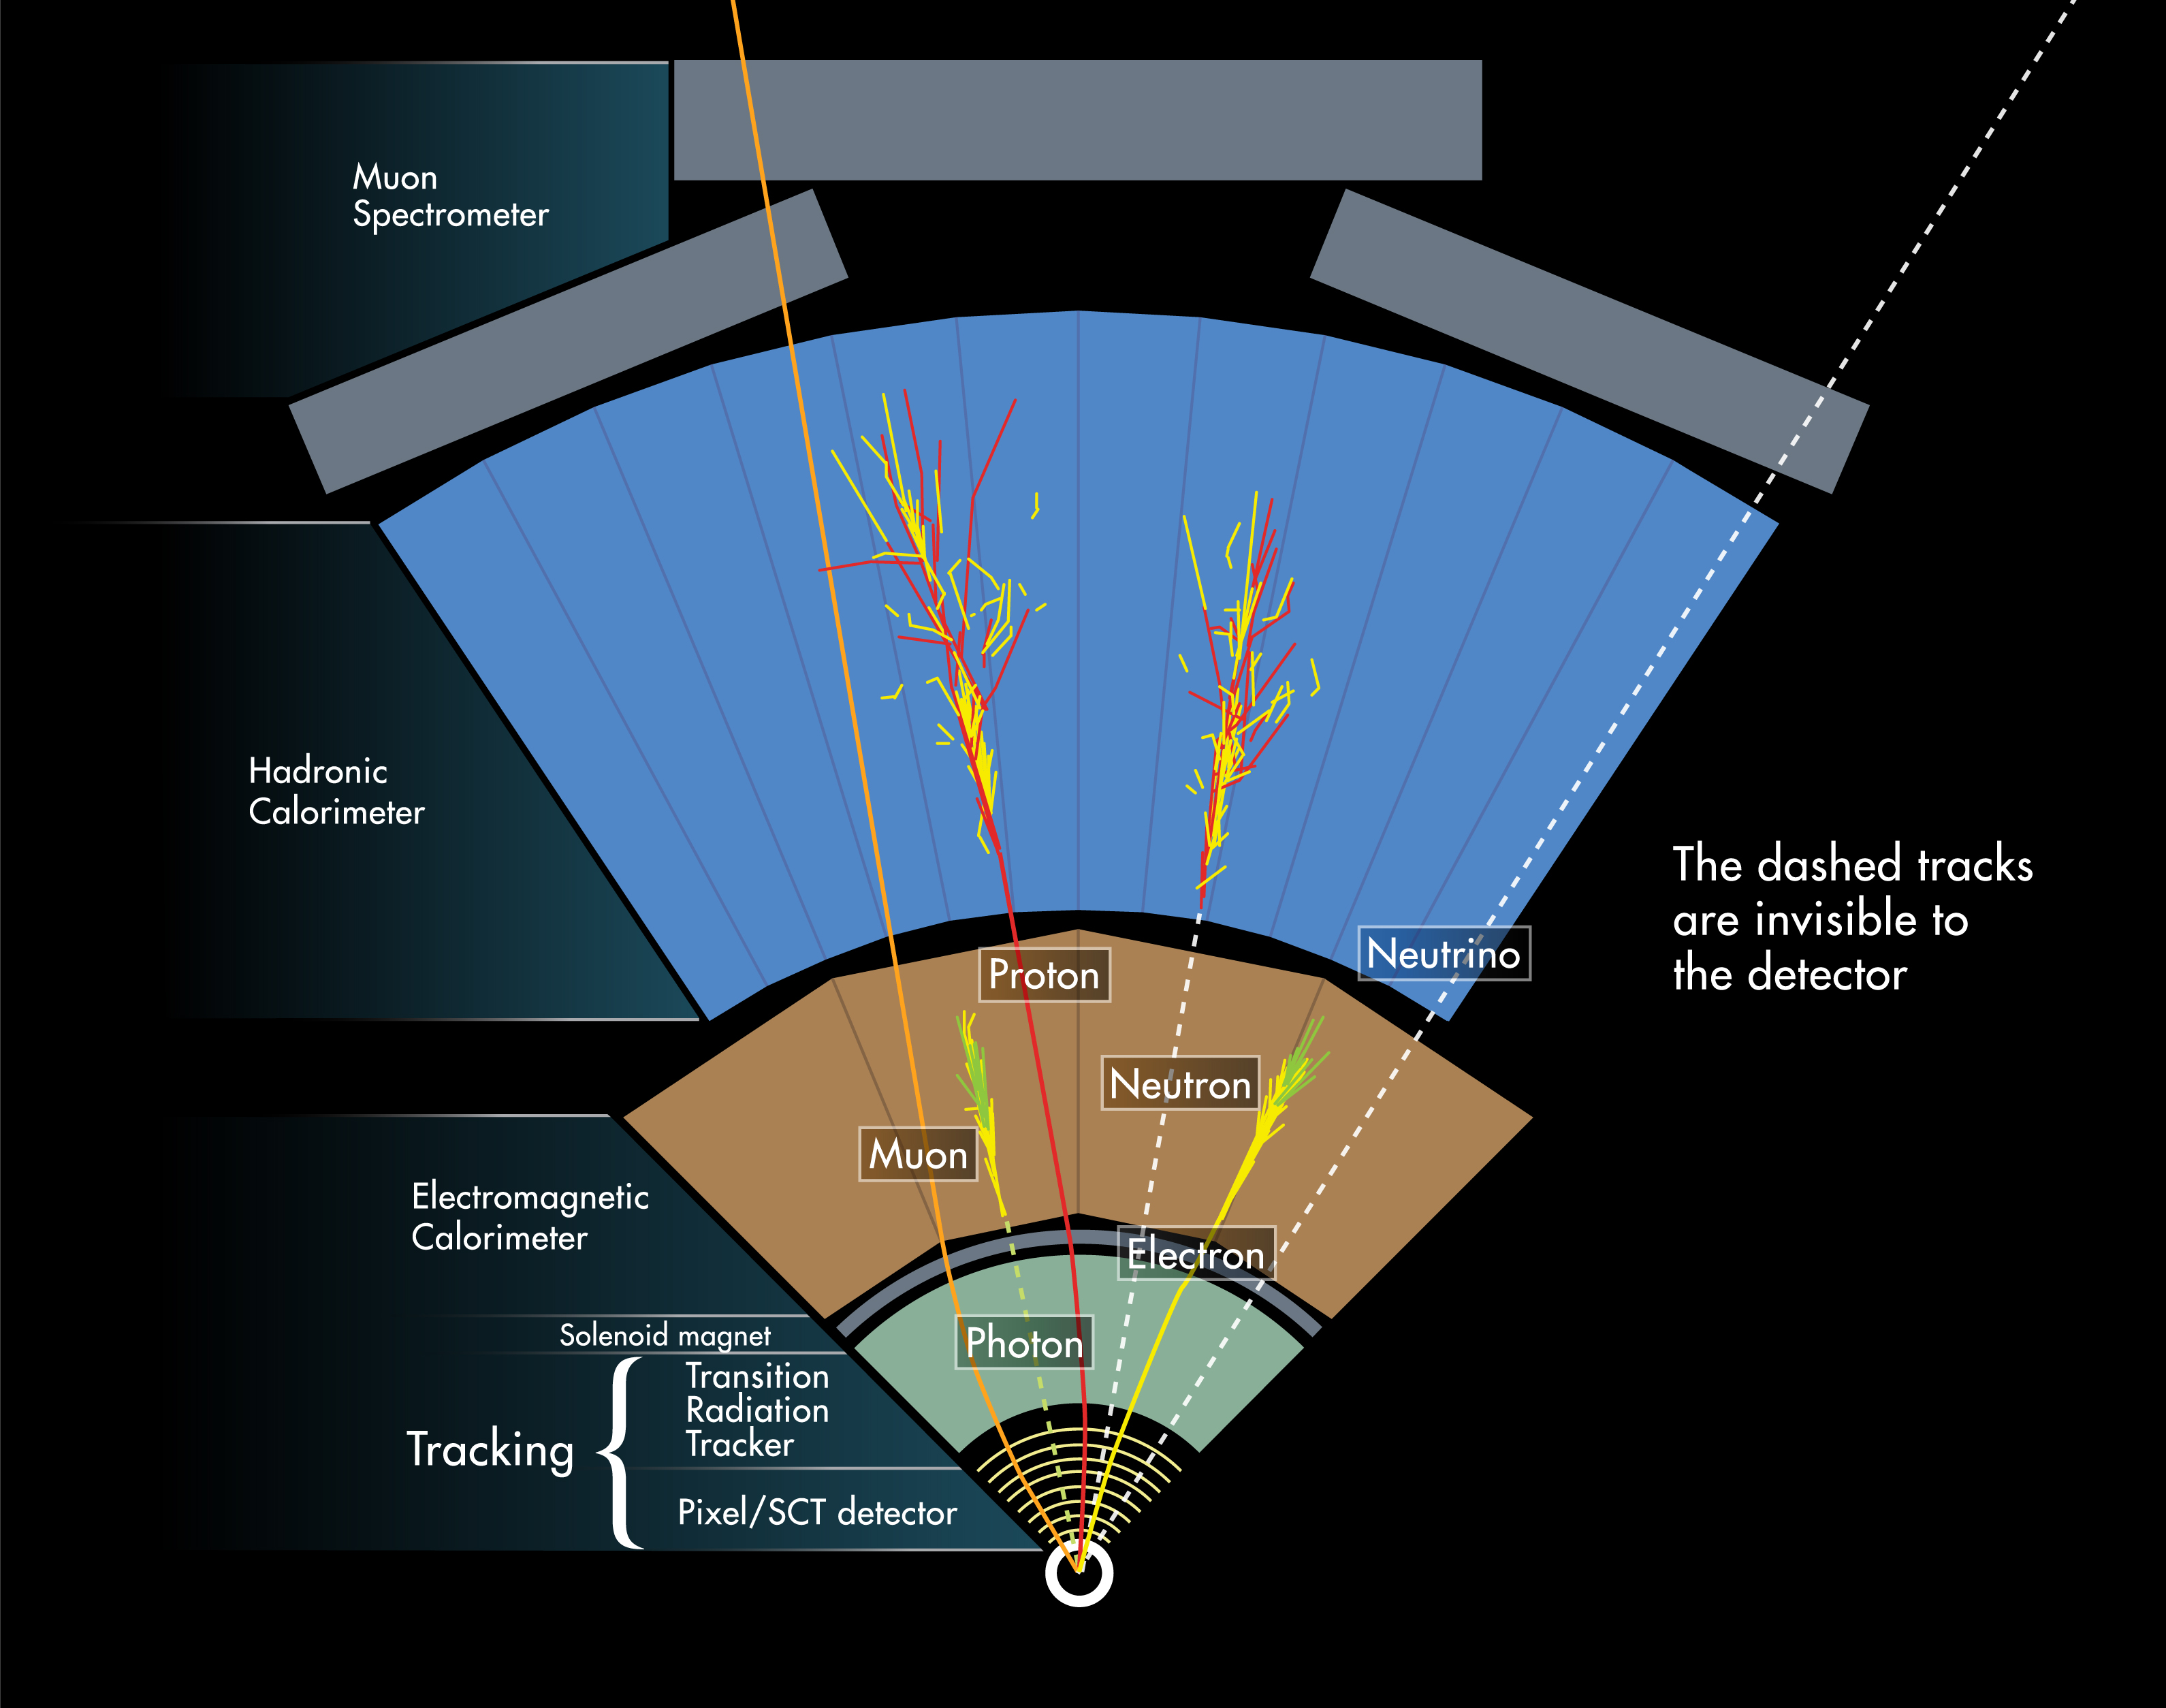
\includegraphics[width=0.85\textwidth, angle=0]{figures/LHC_ATLAS/ATLAS_Signature.jpg}
\caption{ Artistic representation of different detector signatures left by particles in ATLAS.  \label{LHC:fig:ATLASSig}}
%\end{center}
\end{figure}

\indent Details on the reconstruction of physics objects can be found in chapter \ref{chap:reconstruction}.  A brief description of detector signatures will be given here in order to motivate the purpose of each subdetector system. \\

\indent The inner detector provides the position of charged particles as they fly through the detector.  These position measurements are then connected to form a track along the flight path of the charged particle.  A central superconducting solenoid magnet provides a 2 Tesla axial magnetic field that bathes the entire inner detector volume.  The magnetic field bends charged particles in $\phi$ thereby allowing for the measurement of momentum as a function of track curvature.  \\

\indent The calorimeters sample the energy of all charged and neutral particles that interact via the electromagnetic and strong force.   The ATLAS calorimeter is a sampling calorimeter that alternates between absorber and active material layers.   Electromagnetically charged particles such as electrons and photons interact with the dense absorber material mainly through bremsstrahlung, ionization and electron pair production.  An EM particle shower develops until the particles within the shower no longer have the energy necessary to pair produce.  Hadronic particles that interact via the strong force will also form analogous hadronic showers.  The shower particles deposit energy in the active material layers within the calorimeter inducing a signal.  \\


%The particles interact with the dense absorbing material via a number of interactions.  The dominant interaction for electromagnetically charged particles such as the electron is photon emission through bremsstrahlung and ionization.  Neutral high energy photons interact primarily by pair producing electrons.  Any emitted photon and electron will pair produce electrons emit photon until the resulting particles no longer have enough energy to continue the process.  This cascade of particles is called a particle shower.  Hadronic particles that interact via the strong force will also form analogous hadronic showers.  \\

\indent We can measure the longitudinal and lateral shower shape and shower depth by combining signals from different calorimeter layers. Showers from EM objects such as photons and electrons form denser narrow profiles while showers from strongly interacting particles form broad showers that penetrate deep into the hadronic calorimeter. \\

\indent The muon is the only charged SM particle that is expected to be able to fully penetrate the entire calorimeter intact.  Muons in turn leave tracks in the muon spectrometer (MS).  This track can be matched to the inner detector track forming a combined muon track that traverses the entire detector.  Barrel and endcap superconducting toroid magnets provide a magnetic field to the MS volume and allow the momentum measurement.  Field strength varies depending on location but on average an integrated field of 2.5 $T\ddot m$ and 4 $T \cdot m$ are expected for muons traversing through the barrel and endcap respectively.\\

\indent A combination of these different detector signatures is used to identify and reconstruct the different particles produced in a particle collision.  Electrons leave an electromagnetic shower in the calorimeter with an associated track.  Unconverted photons leave an electromagnetic shower without an associated track.  Colored partons fragment into jets and leave a hadronic shower in the calorimeter with a number of associated inner detector (ID) tracks.  Muons are reconstructed from a combined ID and MS track with limited energy deposited in the calorimeter.  Tau leptons either decay leptonically via $\tau \rightarrow \nu \mu \nu$ or $\tau \rightarrow \nu e \nu$ or decay hadronically to pions and leave a narrow hadronic shower in the calorimeter.  Particles that only interact via the weak force, i.e. neutrinos, do not interact with the ATLAS detector.  These weakly interacting particles escape the detector completely and their presence can be inferred through the conservation of transverse momenta as $\met$.\\

\indent The following subsections are dedicated to covering each subdetector in further detail. \\

\subsection{ Inner Detector }
\label{LHC:ID}

\indent The inner detector consists of three independent sub-detectors.  All 3 sub-detectors are immersed in a 2 T axial magnetic field produced by a solenoidal superconducting magnet.  Two silicon semiconductor detectors, the Pixel detector and the Semiconductor Tracker (SCT), form the inner part of the tracking volume and the Transition Radiation Tracker (TRT) covers the outer part.  The three independent sub-detectors together provide a precise and robust pattern recognition system used to reconstruct charged particle tracks and measure charged particle momentum.  The ID also provides precise impact parameter measurements of tracks and primary and secondary vertex reconstruction.   \\

\indent The layout of the inner detector can be seen in Figure \ref{LHC:fig:ATLASID}.  A summary of the geometry and coverage of each ID subdetector is given in Table \ref{tab:IDspec}.  \\

\begin{table}[h!]
  \caption{ Main specifications of each subdetector in the ATLAS inner detector including the intrinsic accuracy of single sensor elements. }
  \label{tab:IDspec}
  \begin{center}
    \begin{tabular}{l c c c} \hline
      Detector & Sensor Element & Avg. num. of hits & $\eta$ coverage \\ 
                     &  Size & per barrel track  & \\ \hline
      IBL         & $50\times240$ $\mu$m$^2$ & 1 & 3.0 \\ 
      Pixel       & $50\times400$ $\mu$m$^2$  & 3 & 2.5\\ 
      SCT        & 80 $\mu$m & 4 & 2.5\\ 
      TRT        &  4 mm & 36 & 2.0 \\ \hline
    \end{tabular}
  \end{center}
\end{table}

\begin{figure}[h!]
%\includegraphics[width=0.45\textwidth, angle=0]{figures/LHC_ATLAS/ID_newTRT_d3.eps}
  \begin{center}
    \begin{subfigure}[a]{0.85\textwidth}   
	\includegraphics[width=\textwidth, angle=0]{figures/LHC_ATLAS/FigID11blast.eps}
         \caption{ }
    \end{subfigure}
    \begin{subfigure}[b]{0.85\textwidth}   
	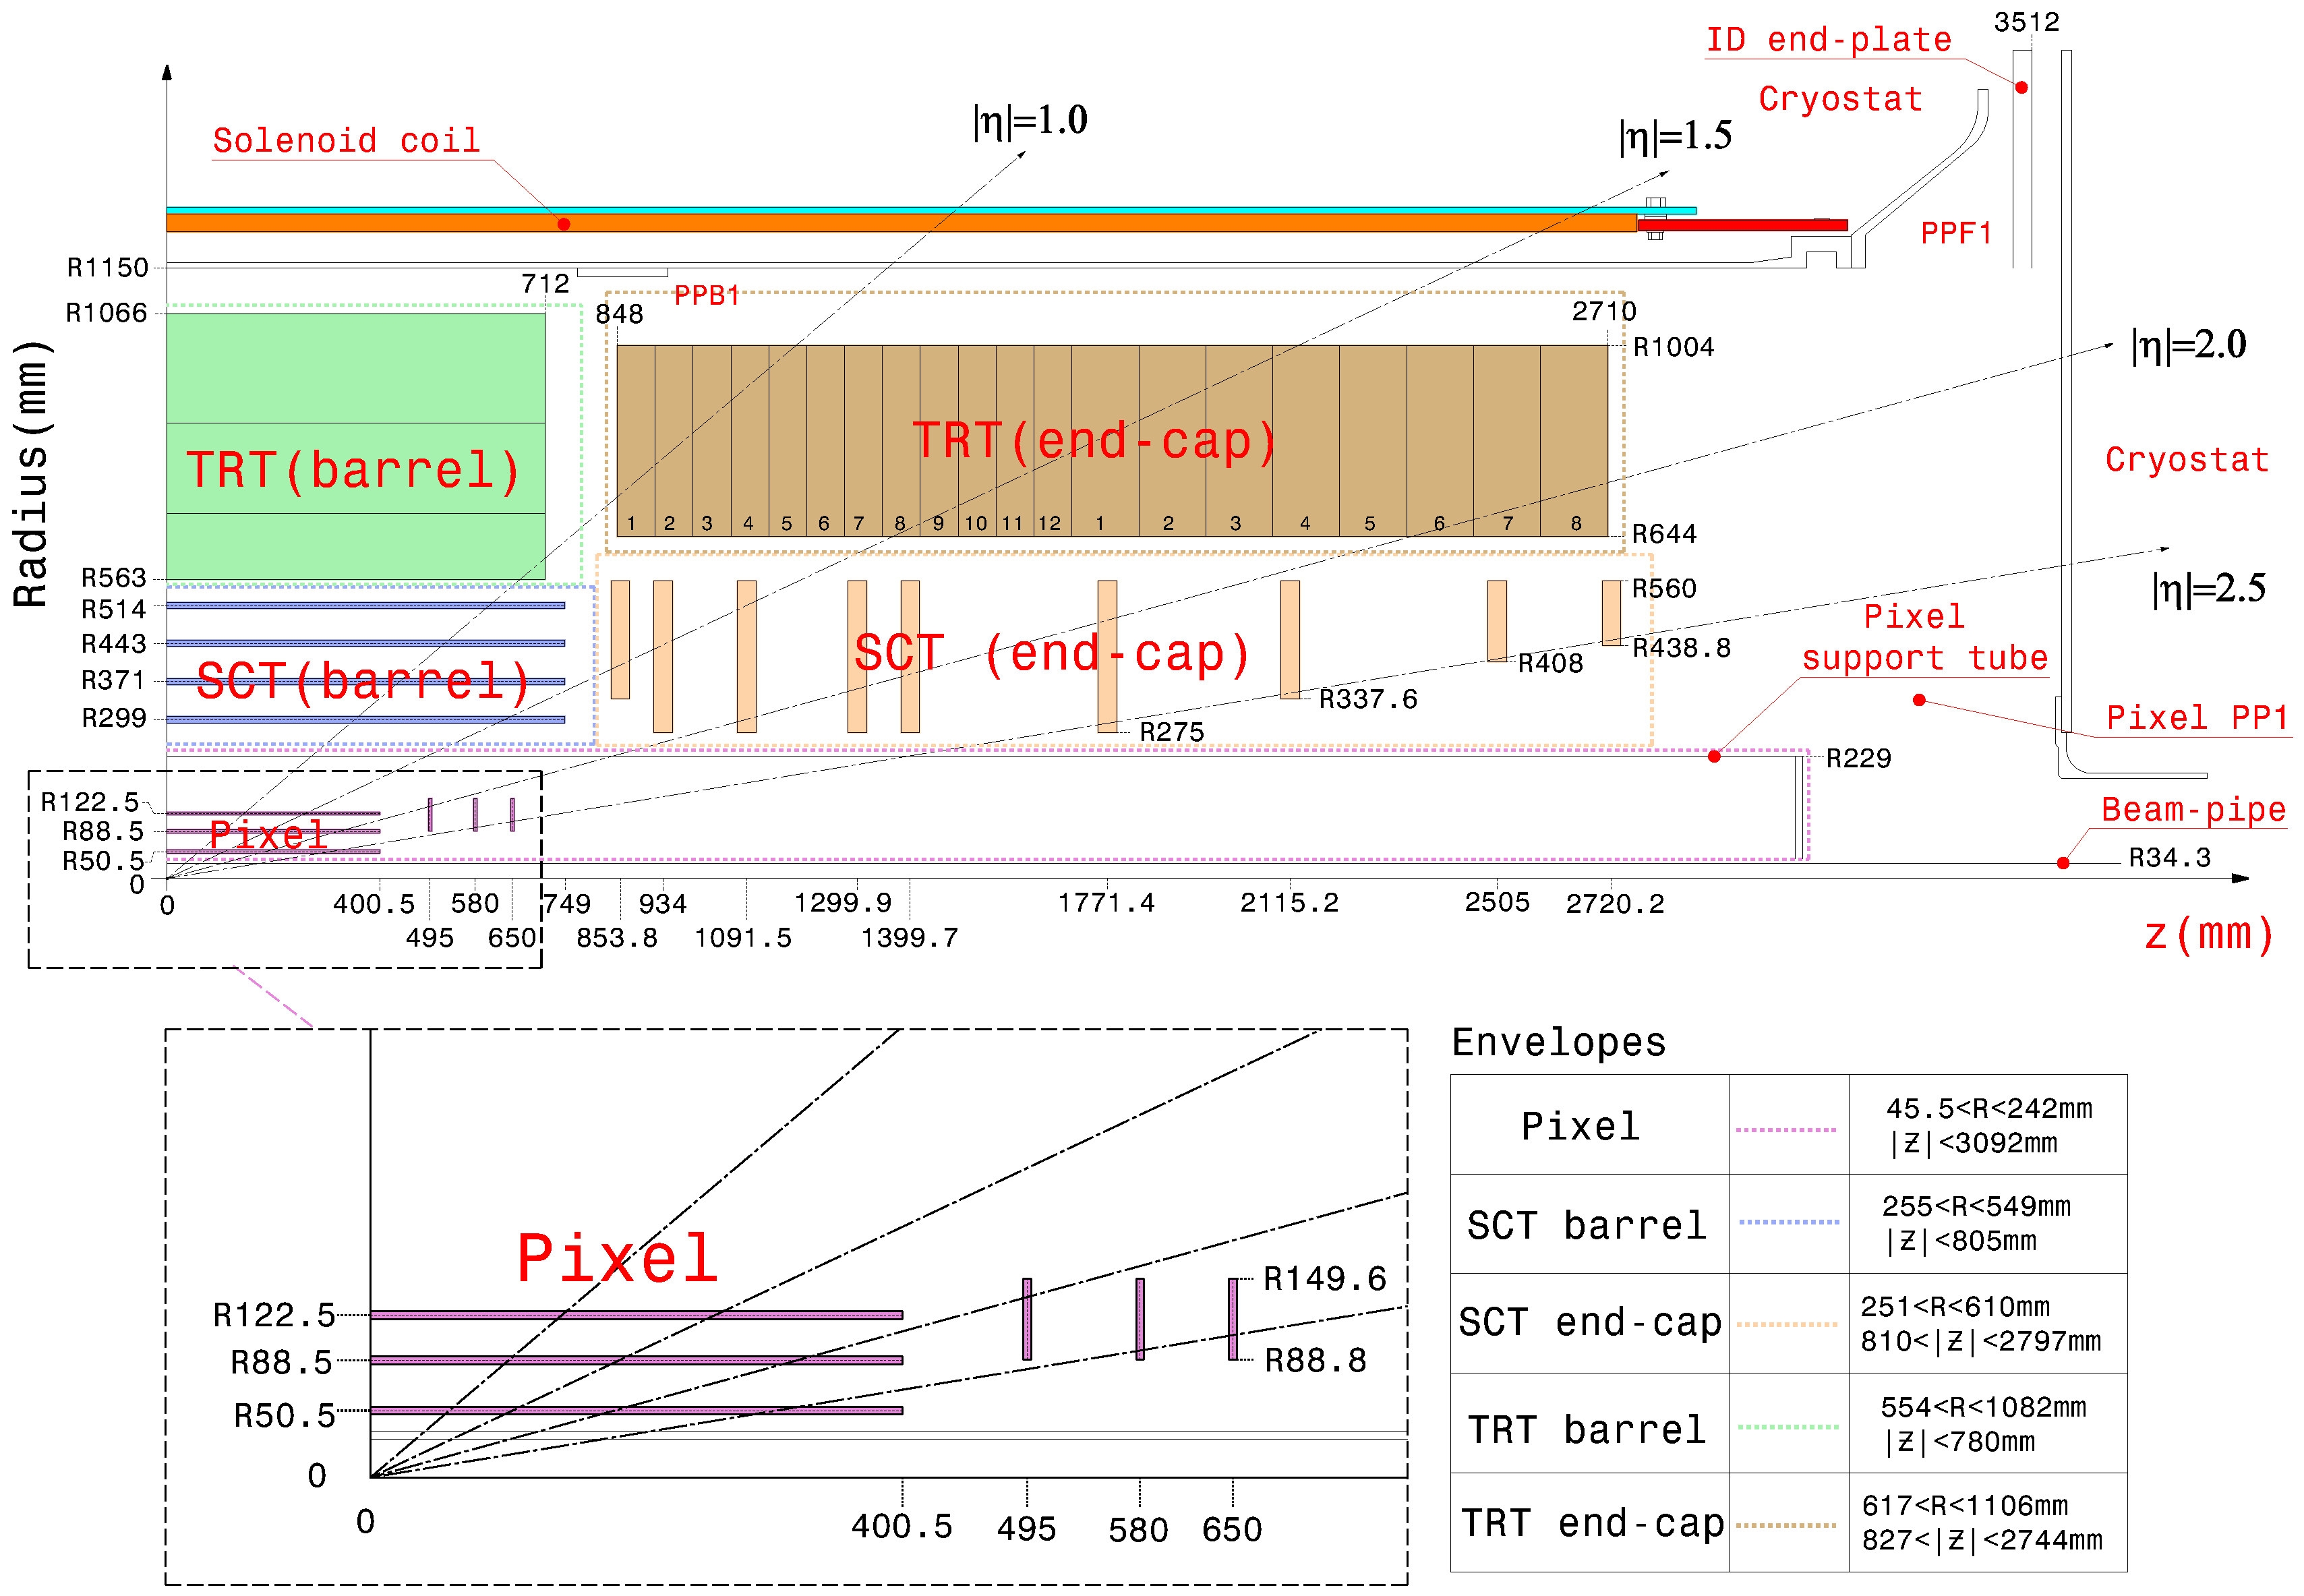
\includegraphics[width=\textwidth, angle=0]{figures/LHC_ATLAS/FigID26-mod-011107.eps}
         \caption{ }
    \end{subfigure}
\caption[~Radial and Cutaway view of the ATLAS inner detector]{ (a) Cutaway view of the ATLAS inner detector. (b) Radial View of the ATLAS inner detector. \cite{ATLAS_JINST} \label{LHC:fig:ATLASID}}
\end{center}
\end{figure}

\indent More detail on each ID sub-detector technology is given below. \\

\subsubsection*{ Pixel Detector and the Insertable B-Layer}

\indent The Pixel detector consists of three layers of high resolution pixel silicon sensors in the cylindrical barrel and three wheels of pixel sensors in the endcap.  The innermost layer of pixel sensors, called the Insertable B-Layer (IBL), was added in the first long shutdown between 2012 and 2015 along with a new beryllium beam pipe.  The new beam pipe decreases the amount of multiple scattering before the inner tracker. \\

\indent The original 3 layer Pixel detector comprises 80.4 million readout channels spread over 1744 Pixel modules.  Each module houses a sensor tile with an area of $63.4 \times 25.4$ mm$^2$.  The sensors are composed of 250 $\mu$m thick n-type silicon wafer pixels with a size of $50\times400 \mu$m$^2$. The modules are read out by 16 front-end electronic chips, each with 2880 read out channels. \\

\indent The pixels have an intrinsic accuracy of 10 $\mu$m in the bending $\phi$ direction and 115 $\mu$m accuracy in the non-bending $z$ direction in the barrel and $\phi$ direction in the endcap.\\ 

\indent Installed in 2014, the Insertable B-Layer (IBL) contributes another 12 million channels to the Pixel system in Run 2.\cite{IBLOverview,IBL_TDR}  Located directly on top of the beam pipe at 3.3 cm from the beam axis, the IBL is the new most inner layer of the Pixel detector ( the previous innermost B-Layer was at 5 cm ). A schematic representation of IBL stave relative to the beam pipe can be seen in Figure \ref{LHC:fig:IBL}. \\

\begin{figure}[h!]
%\begin{center}
\centering
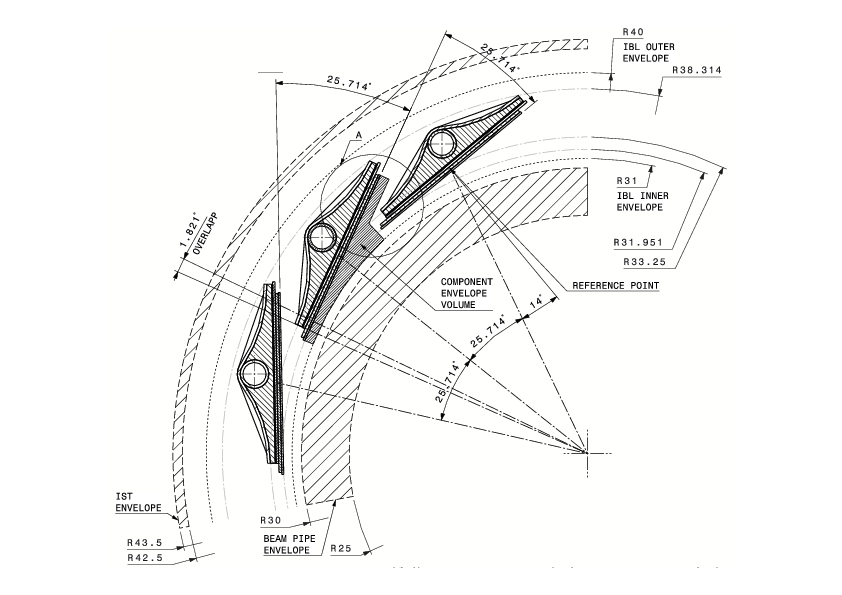
\includegraphics[width=0.85\textwidth, angle=0]{figures/LHC_ATLAS/fig_ibl_layout_rev.png}
\caption[~Schematic of the ATLAS Insertable B-Layer (IBL)]{ Schematic of the ATLAS Insertable B-Layer (IBL).\cite{IBLOverview} \label{LHC:fig:IBL}}
%\end{center}
\end{figure}

\indent The IBL is composed of 14 staves tilted at $14^{\circ}$ in $\phi$.  Each stave is equipped with 32 FE-I4 front-end chips bonded to silicon sensors. Each FE-I4 chip contains 26880 pixel cells with $50 \times 240$ $\mu$m$^2$ pitch.\\

\indent The IBL improves both the tracking lever arm and track spatial resolution.  The combined improvements translate to a factor of $\sim2$ improvement in the impact parameter resolution and a factor of $\sim4$ improvement in the b-tagging light jet rejection power. \\

\subsubsection*{ Semiconductor Tracker}

\indent The SCT is composed of 4 coaxial layers of concentric cylinders in the barrel and 9 disks in each endcap and contributes at least 4 additional layers of high precision position measurements to tracks.  The entire SCT consists of approximately 6.3 million readout channels spread over 4088 modules.  A barrel module is equipped with $64.0 \times 63.6$ mm$^2$ sensors orientated in the transverse plane.  Barrel sensors are made of 285 $\mu$m thick silicon wafers and contain 768 strips, achieving a barrel strip-pitch of 80 $\mu$m.  The endcap modules contain sensors that are trapezoidal in shape with strip pitch that vary from 54 $\mu$m to 90 $\mu$m.  \\

\indent The sensors are mounted in a back-to-back fashion at angle of $40$ mrad relative to one another.  This allows the measurement of non-bending direction along with improved spatial resolution in the bending $\phi$ direction. The intrinsic accuracy per SCT module, dictated by the strip pitch, is 17 $\mu$m in the bending $\phi$ direction and 580 $\mu$m in the non-bending direction.\\

\subsubsection*{Transition Radiation Tracker}

\indent The TRT is the outermost component of the ID and contributes approximately 351000 readout channels.  Each channel corresponds to a 4 mm diameter polyimide straw drift tube with a $31 \mu$m gold plated tungsten anode wire, providing an intrinsic accuracy of 130 $\mu$m.  The total channel number is low compared to the silicon detectors but the TRT is able to compensate for this by providing a long lever arm and high hit multiplicity.  \\

\indent In the barrel region, TRT straws are 144 cm long and arranged parallel to the beam axis in 73 layers. In the end-cap region, straws are 37 cm long and arranged in wheels with 160 radial layers.  A typical barrel track will traverse 36 straws because the tubes are arranged in a matrix with layers offset from one another.\\

\indent The dielectric material used to interweave the straws induces transition radiation in traversing charged particles.  The Xenon-based gas mixture in the straws absorbs the low energy transition radiation photons. The transition radiation thereby induces a much larger signal amplitude than a minimum-ionizing charged particle.  The large signal can then be used to distinguish electrons from charged pions.  \\

\indent In 2015 and 2016, approximately $1/3$ to $2/3$ of the TRT barrel and $1/7$ of the TRT endcap were filled with an Argon gas mixture instead of Xenon due to leakages.  This decreased electron identification efficiency by a few percent during 2015 and 2016.  This decrease in electron identification efficiency is taken into account by a scale factor in the simulation.  \\

\subsection{The Calorimeter}
\label{LHC:Calorimeter}

\indent The ATLAS calorimeter provides near full solid angle coverage of the interaction point up to an $|\eta| < 4.9$.  The calorimeter system is composed of two parts; the electromagnetic calorimeter (ECAL) and hadronic calorimeter (HCAL).  Both ECAL and HCAL are sampling calorimeters with different absorber material depending on the detector region.  The ECAL uses liquid argon (LAr) as the active material and HCAL uses both scintillating tiles and liquid argon (LAr) as active materials.  \\

\indent The cutaway view of the ATLAS calorimeter can be seen in Figure \ref{LHC:fig:ATLASCalo}. \\% and a summary of the calorimeter geometry is given in table \ref{} \\

\begin{figure}[h!]
%\begin{center}
\centering
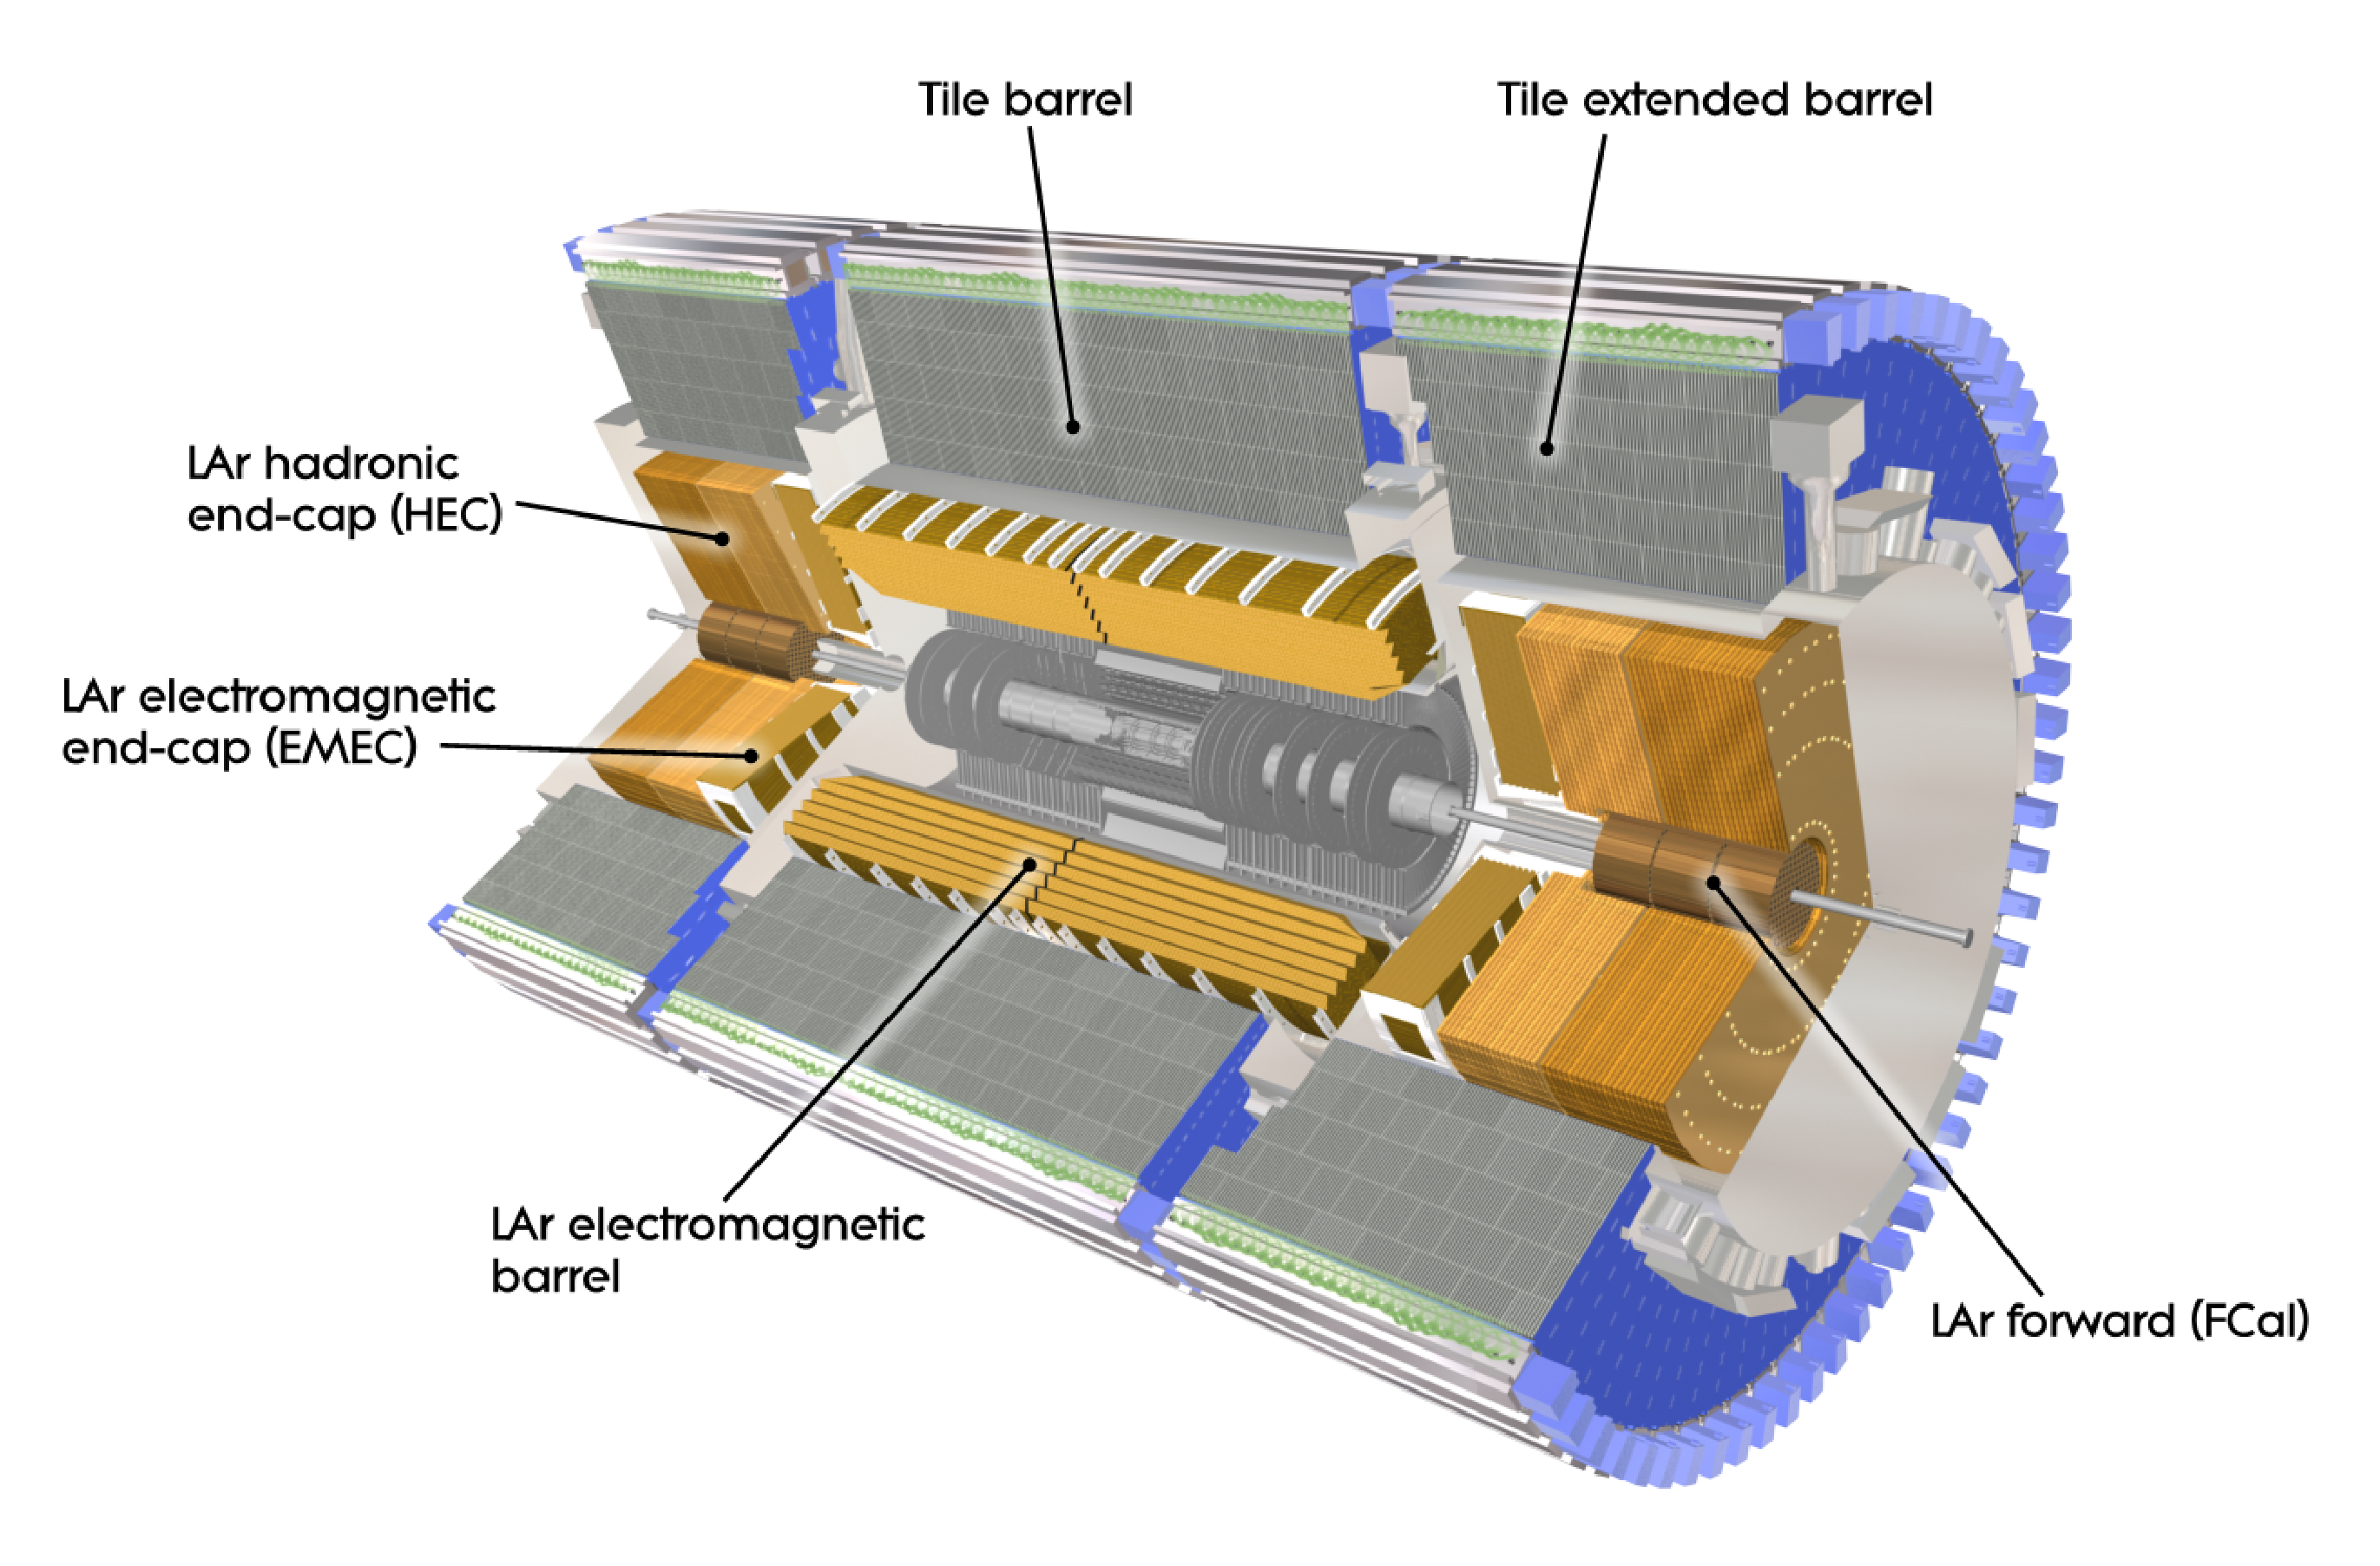
\includegraphics[width=0.75\textwidth, angle=0]{figures/LHC_ATLAS/Calorimeter_d3.eps}
\caption[~Layout of the ATLAS calorimeter]{ Layout of the ATLAS calorimeter.\cite{ATLAS_JINST} \label{LHC:fig:ATLASCalo}}
%\end{center}
\end{figure}

\indent The design EM resolution is $\sigma_E/E = 10\%/\sqrt{E} \oplus 0.2\%$. The design hadronic energy resolution varies from $\sigma_E/E = (56.4\pm0.4)/\sqrt{E}\oplus(5.4\pm0.1)$\% in the barrel region to $\sigma_E/E = (94.2\pm1.6)/\sqrt{E}\oplus(7.5\pm0.4)$\% in the forward regions. \\

\subsubsection*{Electromagnetic Calorimeter}

\indent The ATLAS ECAL is sampling calorimeter with lead absorber plates and LAr active material arranged in an accordion geometry.  The ECAL provides coverage up to an $|\eta| < 3.2 $ and the accordion design gives full crack-less coverage in $\phi$. \\% and integrates more charge along the longitudinal direction of the shower.  \\

\indent The ECAL is split into a barrel and two endcap components with a transition region of $1.37 < |\eta| < 1.52$ in between.  The barrel component is divided into two 3.2 m long half-barrel sections with an inner and outer radius of 2.8 m and 4 m respectively.  The endcap is divided into two coaxial wheels each 63 cm thick with an outer wheel covering the $1.375 < |\eta| < 2.5$ region and an inner wheel covering the $2.5 < |\eta| < 3.2$ region. \\

\indent The barrel ECAL is segmented longitudinally into 3 layers with an additional presampler layer in front of certain regions.  The presampler is composed of a thin liquid-argon layer 11mm in depth and is designed to determine the energy loss from material upstream of the calorimeter.  The first layer after the presampler has a depth of 4.3 radiation length ($\Chi_0$) and a fine granularity with $\Delta\eta \times \Delta\phi = 0.003 \times 0.1$.  The high granularity allows for precision measurement of EM showers and can distinguish between the shower shape of electron/photons from those of $\pi^0\rightarrow \gamma\gamma$ decays.  The middle layer absorbs most of the energy in the EM shower and is made up of cells with $\Delta\eta \times \Delta\phi = 0.025 \times 0.025$ and a depth of $16 \Chi_0$.  The back layer is designed to collect the tails of the EM showers and to distinguish between EM and hadronic showers. The back layer has cell sizes of $\Delta\eta \times \Delta\phi = 0.05 \times 0.025$ and a depth of $2 \Chi_0$.  \\

\indent The endcap ECAL is also divided into three longitudinal layers that perform the functions as the layers in the barrel.  The front layer has a depth of 4.4 $\Chi_0$ and varies in cell size from $\Delta\eta \times \Delta\phi = 0.003 \times 0.1$ to $\Delta\eta \times \Delta\phi = 0.006 \times 0.1$. The middle layer has cells with the same size as the barrel at $\Delta\eta \times \Delta\phi = 0.025 \times 0.025$ and a similar depth. The back layer also has a $\Delta\eta \times \Delta\phi$ of $0.05 \times 0.25$.  A presampler also exists for the endcap with each presampler module consisting of two 2mm thick LAr layers. \\

\indent The ATLAS ECAL segmentation can be seen in Figure \ref{LHC:fig:EMCalo}. \\

\begin{figure}[h!]
\begin{center}
    \begin{subfigure}[b]{0.40\textwidth}   
        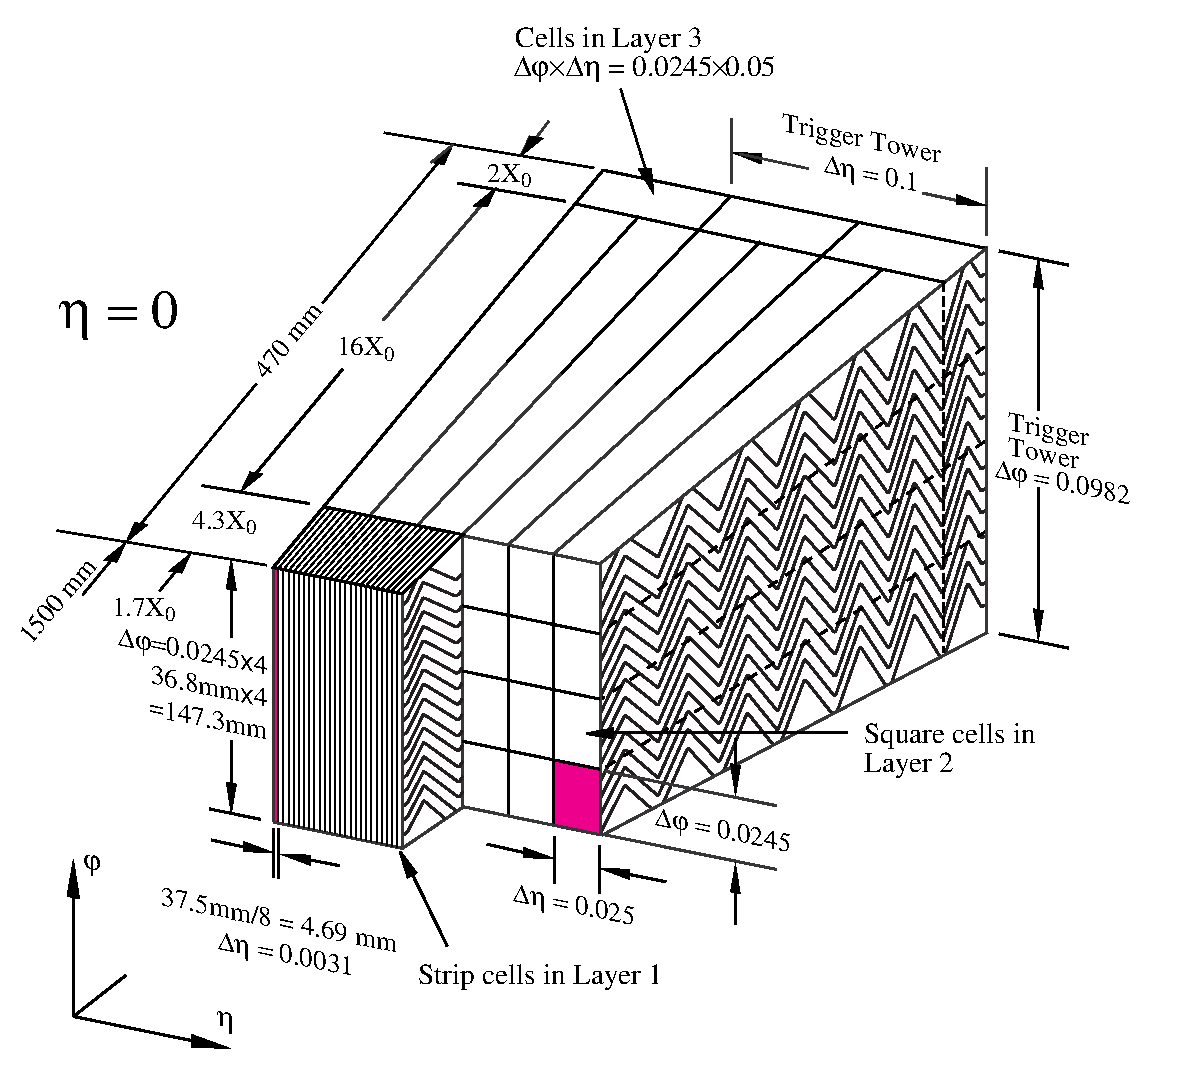
\includegraphics[width=\textwidth, angle=0]{figures/LHC_ATLAS/LARG3-TDR-barrelM.eps}
        \caption{}
    \end{subfigure}
    \begin{subfigure}[b]{0.50\textwidth}
	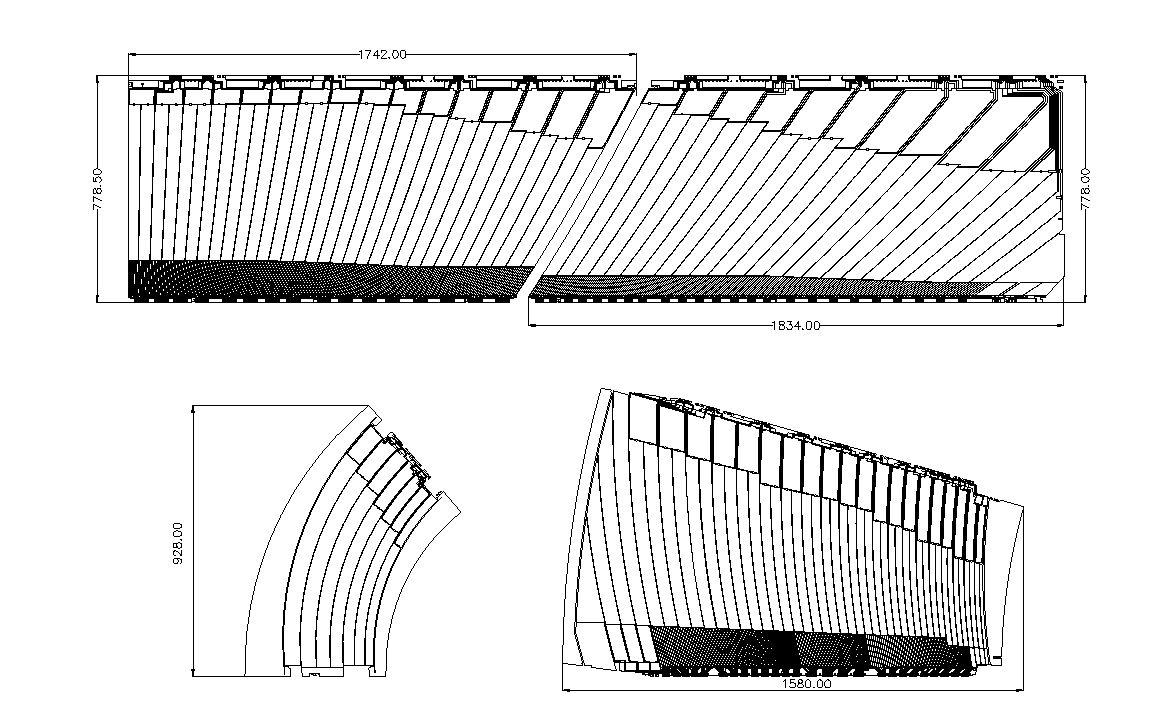
\includegraphics[width=\textwidth, angle=0]{figures/LHC_ATLAS/LARG3-abcdM.eps}
	\caption{}
    \end{subfigure}
\caption[~Schematic depiction of the ATLAS electromagnetic calorimeter module and cells]{ Schematic depiction of the ATLAS electromagnetic calorimeter (a) The three layers of the EM calorimeter module with the accordion geometry shown. (b) Orientation of EM calorimeter cells in the barrel and endcap relative to the IP.  Cells are orientated to point back to the IP.\cite{ATLAS_JINST} \label{LHC:fig:EMCalo}}
\end{center}
\end{figure}

\indent The total thickness of the ECAL is at least $22 \Chi_0$ in the barrel and $24 \Chi_0$ in the endcap for electrons and photons and approximately 1.5 nuclear interaction length for hadronic objects. \\

\subsubsection*{Hadronic Calorimeter}

\indent The ATLAS HCAL is directly outside the ECAL and is responsible for containing and measuring the energy of hadronic showers.  The HCAL consists of 3 separate detectors covering different $\eta$ regions. The tile calorimeter covers the central region with $|\eta| < 1.7$.  The LAr endcap calorimeter (HEC) covers the endcap region with $1.5<|\eta| < 3.2$ and the LAr forward calorimeter (FCal) covers the forward region to upwards of $|\eta| < 4.9$.  \\

\indent The tile calorimeter is a sampling calorimeter using steel absorbers and scintillating tiles as active material. Two separate photomultiplier tubes read out the two sides of the scintillating tiles.  \\

\indent The barrel tile calorimeter covers an $\eta$ range of $|\eta| < 1.0$ and two extended barrel tile calorimeters cover the $0.8 < |\eta| < 1.7$ region.  Both barrel and extend barrel calorimeters are divided into 64 modules orientated along the $\phi$ direction.  Each module covers a $\phi$ region of $\Delta\phi = 0.1$.  The module is segmented in the radial direction into 3 longitudinal layers.  The 3 layers have an approximate thickness of 1.5, 4.1 and 1.8 nuclear interaction lengths ($\lambda$) in the barrel and 1.5, 2.6, and 3.3 $\lambda$ in the extended barrel.  

\indent A Schematic view of a tile calorimeter module can be seen in Figure \ref{LHC:fig:TileCalo}

\begin{figure}[h!]
%\begin{center}
\centering
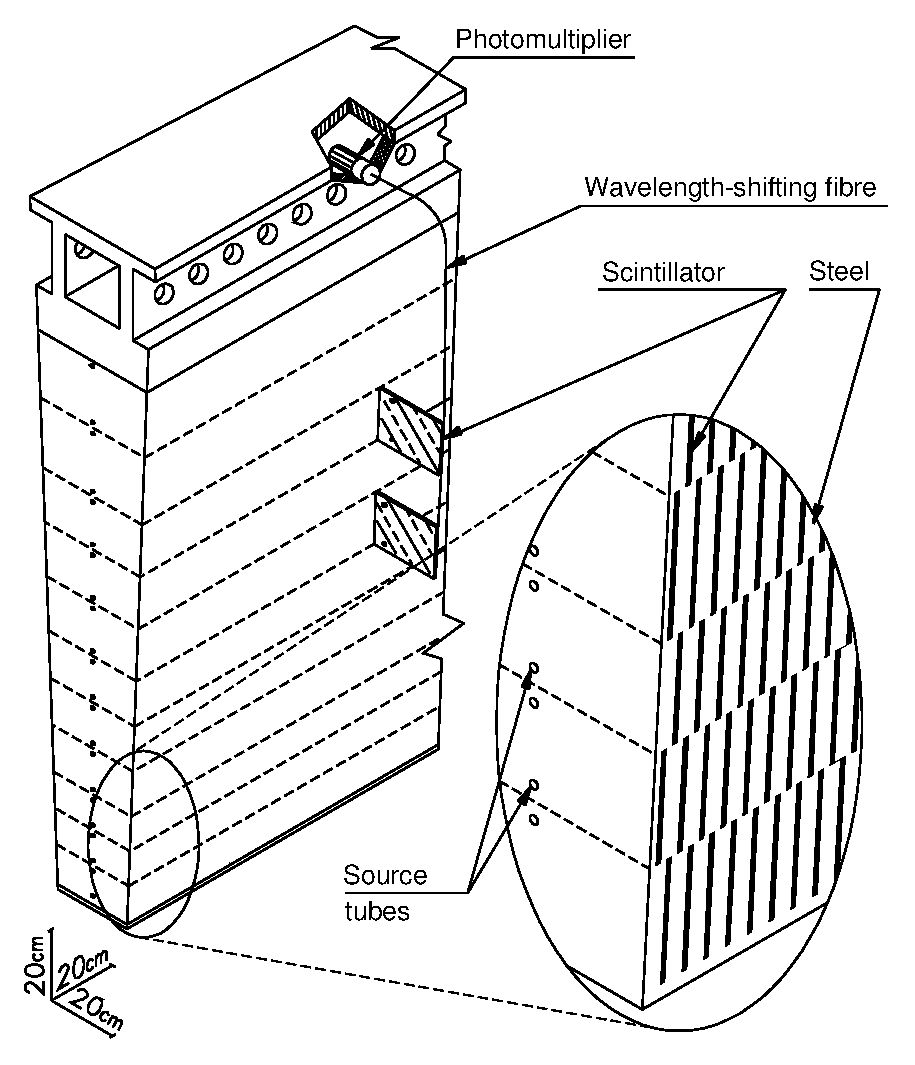
\includegraphics[width=0.45\textwidth, angle=0]{figures/LHC_ATLAS/TileCal_Module3.eps}
\caption[~The tile calorimeter module with steel absorber, tile scintillators and photomultiplier readout]{ The tile calorimeter module with steel absorber, tile scintillators and photomultiplier readout.\cite{ATLAS_JINST} \label{LHC:fig:TileCalo}}
%\end{center}
\end{figure}


\indent The HEC uses LAr as the active material and copper as the absorber with copper plates interwoven between the LAr gaps.  The HEC is located directly behind the ECAL endcap and two calorimeters share a single cryostat.  The HEC  covers an $\eta$ range of $1.5<|\eta| < 3.2$ and overlaps slightly with the tile calorimeter and FCAL in order to minimize any drop in material density.  \\

\indent Geometrically the HEC consists of two independent wheels per endcap with each wheel subdivided into 32 wedge shaped $\phi$ modules.  Each HEC module is composed of cells with a size of $\Delta\eta \times \Delta\phi = 0.1 \times 0.1$ for the $|\eta|<2.5$ region and $\Delta\eta \times \Delta\phi = 0.2 \times 0.2$ in higher eta regions.  The HEC module is also segmented longitudinally into 2 layers making a total of 4 longitudinal layers in the 2 wheels. The combined depth of all 4 layers is approximately 10 interaction lengths. \\

\indent The FCal is an LAr sampling calorimeter that extends the $\eta$ coverage of the HCAL up to $|\eta| < 4.9$.  A compact design with very small LAr gaps is chosen for this high flux region.  The FCal is segmented in the longitudinal direction with 3 distinct modules. The absorber material is copper for the first module and tungsten in the last two.  The copper absorber is optimized for EM measurements while the tungsten is predominantly designed for hadronic interactions.  The 3 modules combined achieve a depth of 10 nuclear interaction length. \\

\subsection{The Muon Spectrometer}
\label{LHC:MuonSpec}

\indent The muon spectrometer (MS) consists of three layers of precision tracking chambers to track the path of muons in the bending $\eta$ direction.  The precision tracking chambers mainly consists of Monitored Drift Tube (MDT) detectors but also includes Cathode Strip Chambers (CSC) in the forward region.  Complementing the precision trackers are fast trigger chambers, the Resistive Plate Chambers (RPC) in the barrel and the Thin Gap Chambers (TGC) in the endcap. \\


\indent The MS is designed to be able to detect muon candidates with a wide range of momenta from $3 \gev$ to $3 \tev$ with standalone muon momentum resolution of $\sigma_{\pt}/\pt = 10\%$ at a $\pt$ of 1 TeV.  The configuration of the MS is shown in Figure \ref{LHC:fig:ATLASMuonSpec}.  The open design of the MS minimizes multiple scattering after the calorimeter and gives a large lever arm for high momentum resolution. ~\\

\begin{figure}[h!]
%\begin{center}
\centering
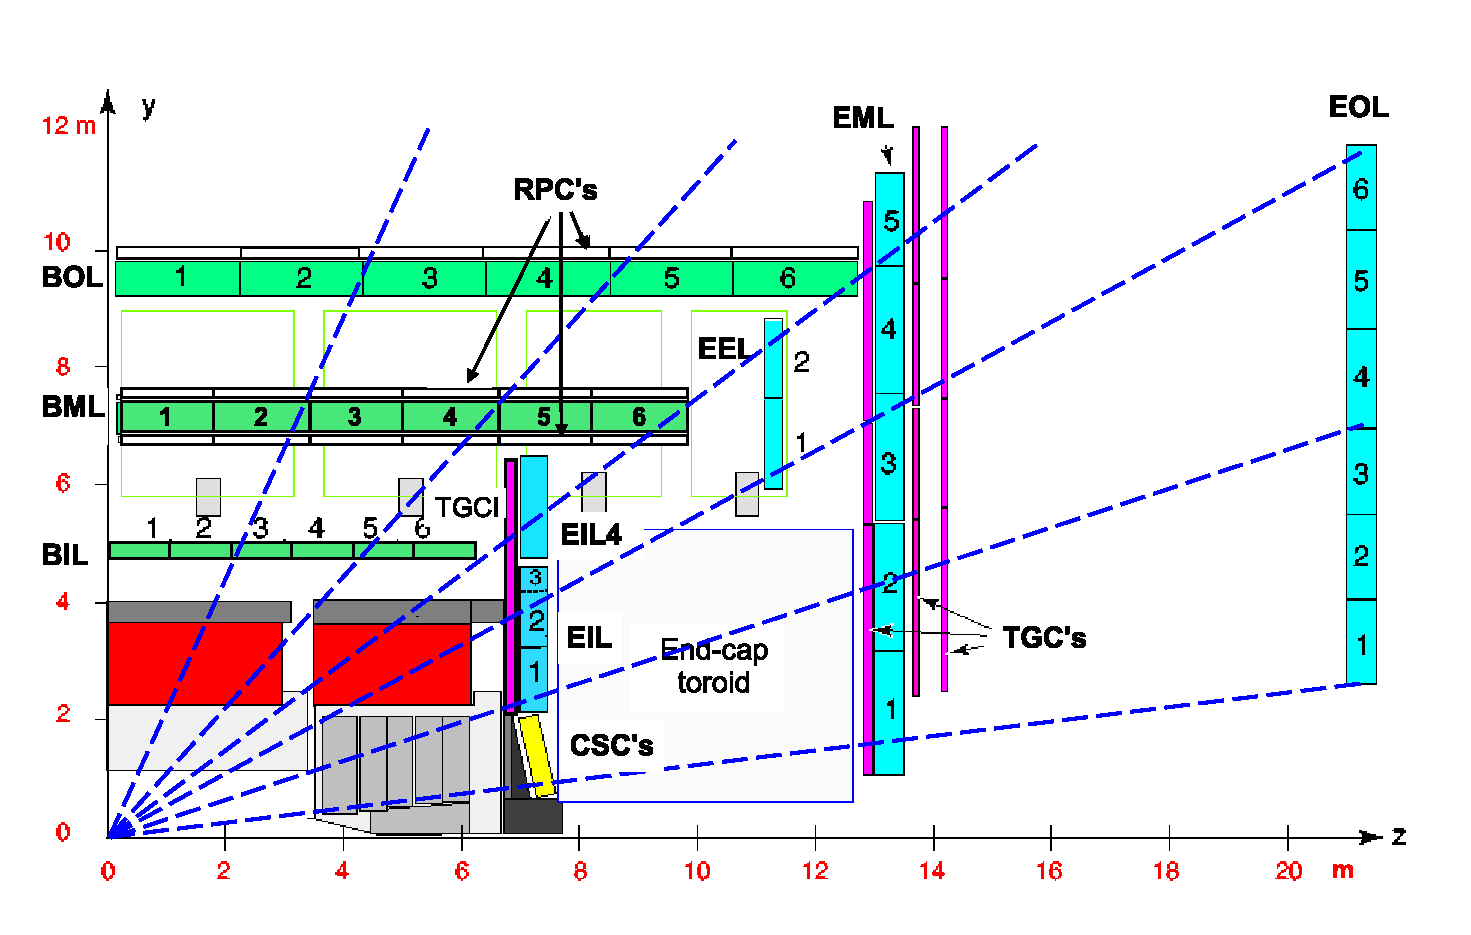
\includegraphics[width=0.75\textwidth, angle=0]{figures/LHC_ATLAS/Muon_rz_large_sect_6.eps}
\caption[~Cutaway view of the ATLAS Muon Spectrometer]{ Cutaway view of the ATLAS Muon Spectrometer.\cite{ATLAS_JINST} \label{LHC:fig:ATLASMuonSpec}}
%\end{center}
\end{figure}

\indent Eight air core superconducting toroid magnets in the barrel and eight additional magnets in each endcap provide a 1.0 $T \cdot m$ to 7.5 $T \cdot m$ of bending power in the MS volume. The configuration of the magnets is shown in Figure \ref{LHC:fig:ATLASMag} ~\\

\begin{figure}[h!]
%\begin{center}
\centering
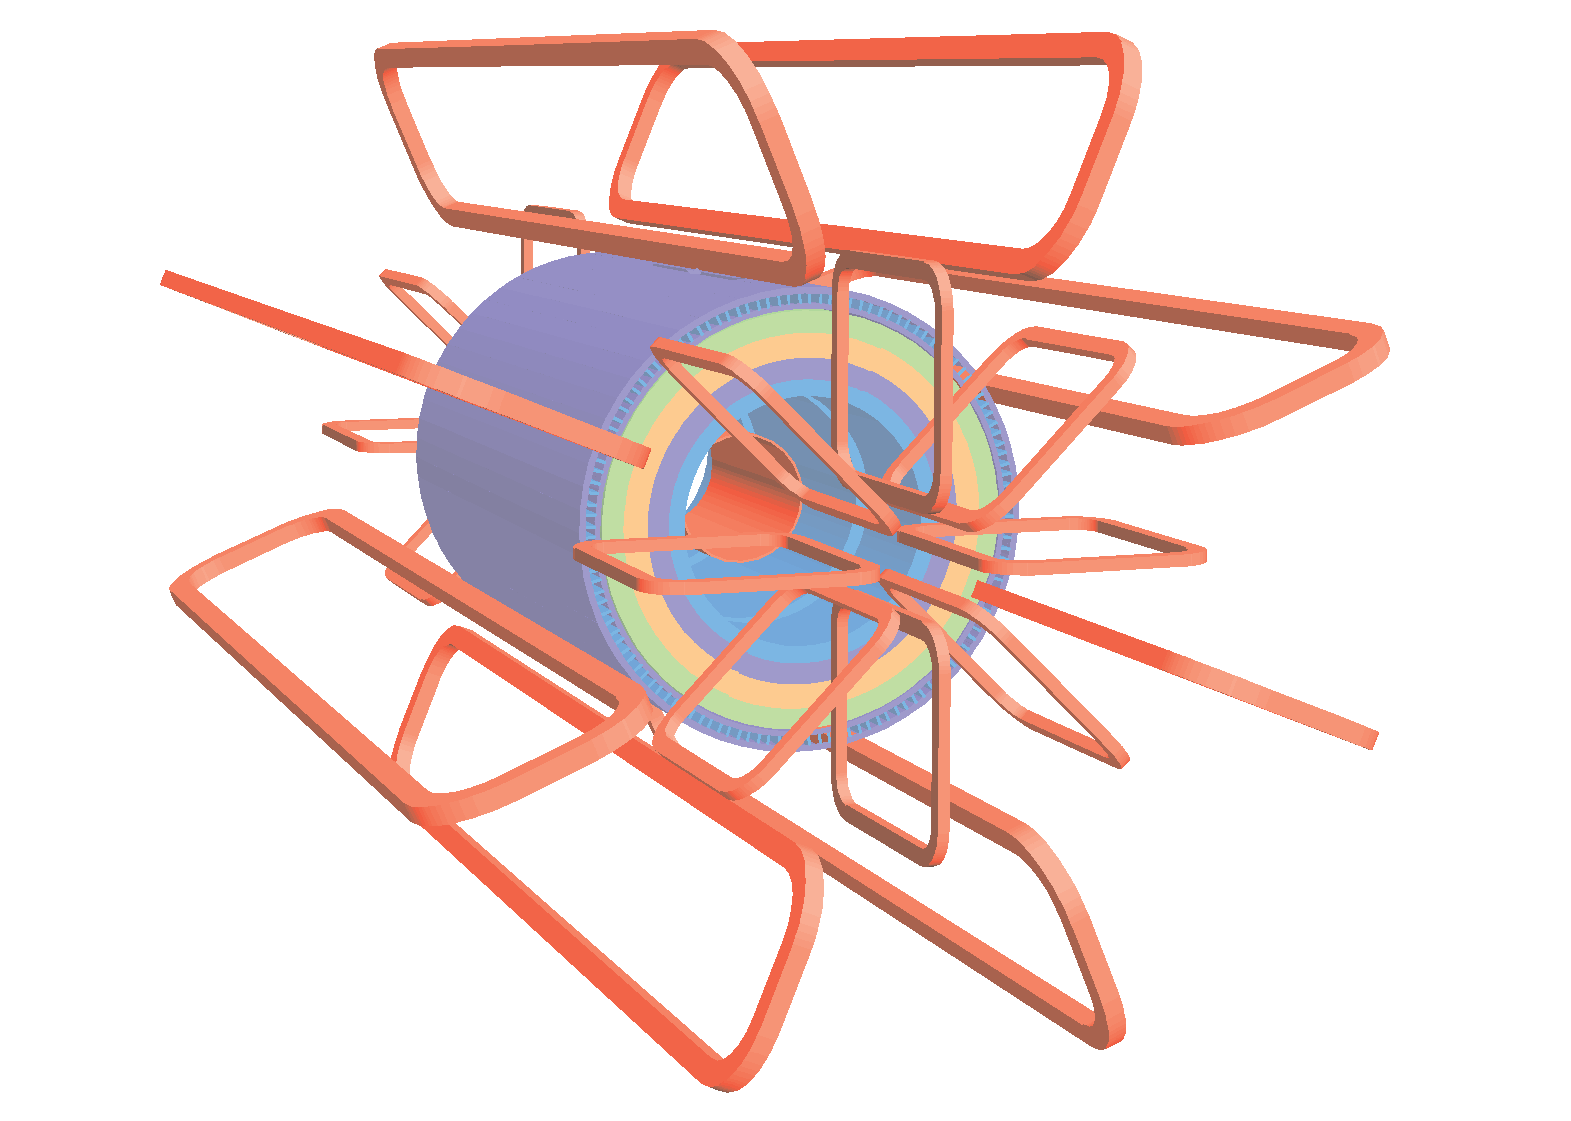
\includegraphics[width=0.60\textwidth, angle=270]{figures/LHC_ATLAS/ATLcoilGeom.eps}
\caption[~Geometry of the ATLAS barrel and endcap toroid magnets]{ Geometry of the ATLAS barrel and endcap toroid magnets. The cylinder represents the calorimeter.\cite{ATLAS_JINST} \label{LHC:fig:ATLASMag}}
%\end{center}
\end{figure}

\indent The barrel magnets cover an |$\eta$| range up to 1.4 and the endcap magnets cover an |$\eta$| range from 1.6 to 2.7. The area between $1.4 < |\eta| < 1.6$, called the transition region, has a mixed magnetic field from both the barrel and endcap. The endcap magnets are offset from the barrel magnets by 22.5 degrees in $\phi$ to allow a smoother magnetic field in the transition region. \\

\subsubsection*{Muon Precision Tracking}

\indent The ATLAS MS system consists of 3 stations of muon precision tracking chambers at approximately 5 m, 7.5 m and 10 m radii in the barrel and 7.4 m,14 m and 21.5 m in $z$ in the endcap.  This provides precision tracking coverage up to an $|\eta| < 2.7$.  Most precision tracking chambers use Monitored Drift Tube (MDT) technology with 3 to 8 layers of MDT tubes each.  The only exception to this is the very high rate forward region with $2.0 < |\eta| < 2.7$ which uses CSC technology. \\

\indent  MDT tubes are 3cm diameter aluminum tubes filled with Ar/CO$_2$ gas mixture with a tungsten-rhenium anode wire.  Each tube has an intrinsic resolution of 80 $\mu$m corresponding to a resolution of $35$ $\mu$m per chamber and offers position measurements in the bending $\eta$ direction.  \\

\indent The CSCs are multiwire proportional chambers with one layer of anode wires in the bending plane and two layers of cathode strips. The position measurement is obtained by interpolating the signal on neighboring cathode strips. The strips are perpendicular to one another with 5.31mm (5.56mm) pitch in the bending plane and 12.5 mm (21.0 mm) in the non-bending plane for small (large) chambers.   This results in a $60 \mu$m resolution per plane in the bending plane and about 5 mm resolution in the non-bending plane. \\ %The CSC wire signals are not read out.    The primary limiting factor for the CSC spatial resolution is electronic noise of the pre-amplifiers and not strip pitch. 

\indent The structure of MDT tubes and CSC chambers can be seen in Figures \ref{LHC:fig:MDT} and \ref{LHC:fig:MDT} . \\

\begin{figure}[h!]
%\begin{center}
\centering
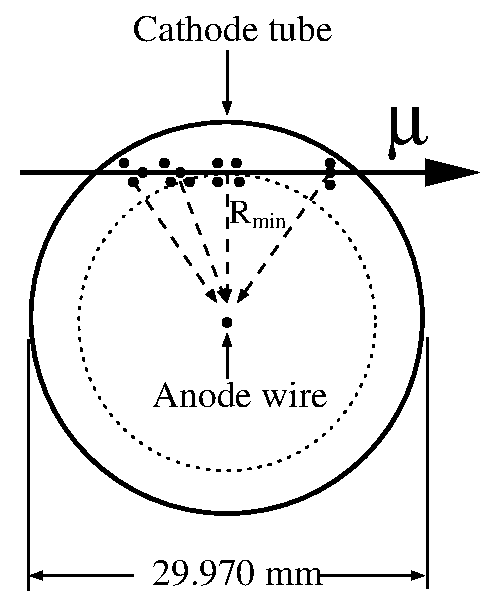
\includegraphics[width=0.30\textwidth, angle=0]{figures/LHC_ATLAS/MDT_tube_cross_section.eps}
\caption[~Schematic Representation of MDT tubes]{ Schematic Representation of MDT tubes.\cite{ATLAS_JINST} \label{LHC:fig:MDT}}
%\end{center}
\end{figure}

\begin{figure}[h!]
%\begin{center}
\centering
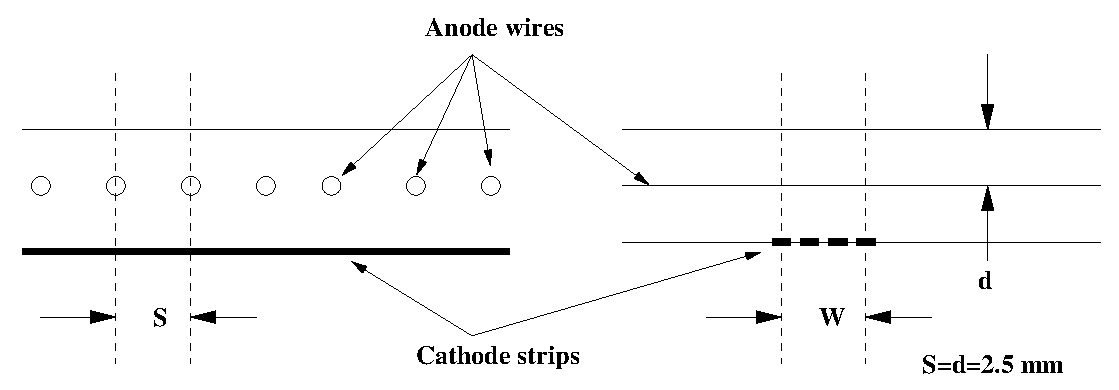
\includegraphics[width=0.85\textwidth, angle=0]{figures/LHC_ATLAS/CSC_structure.eps}
\caption[~Schematic Representation of CSC chambers]{ Schematic Representation of CSC chambers.\cite{ATLAS_JINST} \label{LHC:fig:MDT}}
%\end{center}
\end{figure}

\subsubsection*{Muon Trigger Chambers}

\indent  The ATLAS MS also features a system of fast trigger chambers consisting of three stations of Resistive Plate Chambers (RPC) in the barrel and 4 stations of Thin Gap Chambers (TGC) in the endcap.  The MS triggering system provides triggering coverage up to an $|\eta|$ of 2.4.  The RPCs are placed below and above the middle MDT station and outside the outer MDT barrel station.  The TGC stations are arranged with one station in front of the inner endcap precision tracking wheel and 3 stations split in front and behind the middle endcap MDT wheel.  \\

\indent In Run 2, muon triggers in the endcap also require coincidences in the inner-most layer of the TGC to reduce fake trigger rates due to particles interacting with beam shielding in the forward region. \\

\indent A schematic of the muon trigger system is given in Figure \ref{LHC:fig:MS_trigger}. The trigger searches for fast coincidences between the layers along the expected trajectory of a muon.  Different maximum deviation from the straight infinite momentum path is allowed for triggers with different $\pt$ thresholds. \\

\begin{figure}[h!]
%\begin{center}
\centering
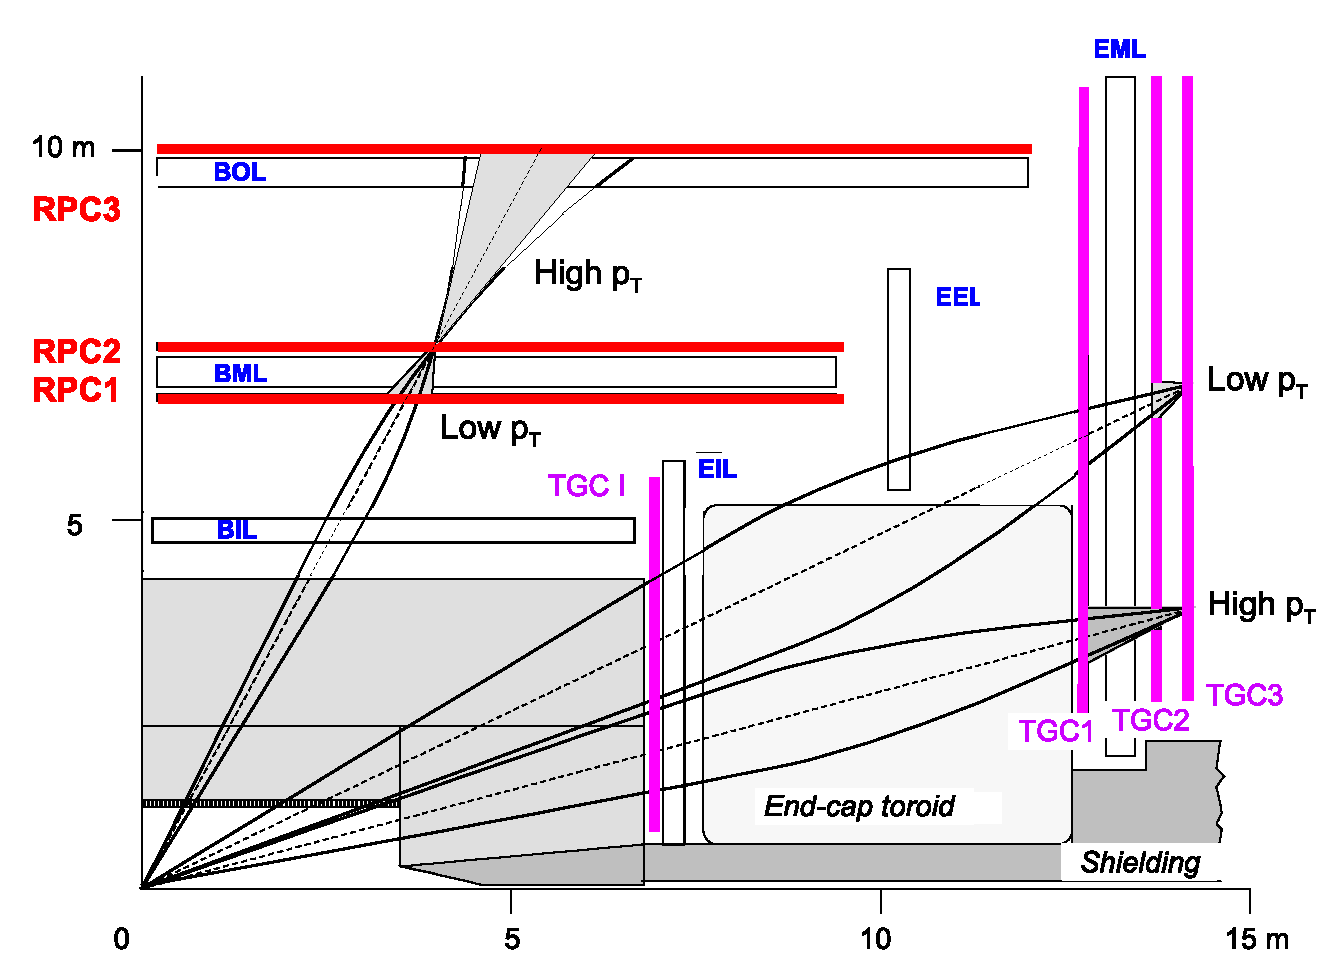
\includegraphics[width=0.75\textwidth, angle=0]{figures/LHC_ATLAS/RPC_TGC_schematics_5.eps}
\caption[~Schematic of the ATLAS muon trigger system]{ Schematic of the ATLAS muon trigger system.  The coincidence windows for muons of different $\pt$ is shown.\cite{ATLAS_JINST} The trigger searches for fast coincidences between the layers along the expected trajectory of a muon.  Different maximum deviation from the straight infinite momentum path is allowed for triggers with different $\pt$ thresholds. High $\pt$ tracks are straighter and lie closer to the infinite momentum straight track than a low $\pt$ track.  \label{LHC:fig:MS_trigger}}
%\end{center}
\end{figure}

%\chap{Experimental Apparatus}
\label{chap:detector}
\section{The Large Hadron Collider}
\indent The Large Hadron Collider (LHC) is the world's most powerful particle accelerator. By accelerating protons to 99.9999991 percent of the speed of light and smashing them in head on collisions, the LHC hopes to probe some of the most fundamental questions of physics. The LHC sits in a circular tunnel 27 km in circumference under the Franco-Swiss border near Geneva, Switzerland. A diagram of the LHC complex is shown in figure \ref{LHC:fig:LHCComplex} ~\\
\begin{figure}[h!]
%\begin{center}
\centering
\includegraphics[width=0.85\textwidth, angle=270]{plots/AccComplex0700829.pdf}
\caption{ The Large Hadron Collider complex. (Taken from \cite{biblio:LHCpublic}) \label{LHC:fig:LHCComplex}}
%\end{center}
\end{figure}

\indent The LHC expands upon older particle accelerators. First protons are obtained by stripping electrons from hydrogen atoms. These protons are accelerated by LINAC2, a older linear accelerator at CERN, to 31.4 percent of the speed of light. The Proton Synchrotron Booster (PSB) then boosts the protons to 91.6 percent of the speed of light. These protons are then dumped into the Proton Synchrotron (PS) and accelerated to 99.93 percent of the speed of light. Afterwards, the protons enter the Super Proton Synchrotron (SPS). The SPS accelerate the proton to 99.9998 percent of the speed of light. At this point the energy of the proton is 450 GeV. These protons finally enter the LHC ring, which increases the proton energy to 3.5 TeV. This allows for a center of mass energy of 7 TeV during collisions. ~\\
\indent The LHC is designed to accelerate the protons to energies of 7 TeV, creating 14 TeV center of mass collisions. The LHC is scheduled to achieve this target energy in two years. ~\\
\indent The LHC has six particle detectors to detect the multitude of particles that are created during the collisions. The ALICE detector specializes in collisions of heavy ions. LHCb specializes in physics involving the bottom quark. TOTEM and LHCf are detectors measuring scattering cross sections, and diffractive processes, and cosmic ray physics. ATLAS and CMS are general purpose detectors optimized to detect a large spectrum of particles created by the proton proton collision. ~\\
\indent This analysis uses data collected by the ATLAS detector. ~\\
\section{The ATLAS Detector}
\label{LHC:detector}
\indent The ATLAS Detector is a general purpose detector that detects a multitude of particles that is created by the proton proton collisions. The detector is 25 meters high and 44 meters long and weights over 7000 tons.\cite{biblio:JINST} The detector consists of an inner tracking detector, the electromagnetic calorimeter, the hadronic calorimeter and the muon spectrometer. The structure of the ATLAS detector is shown in figure \ref{LHC:fig:ATLASDet} ~\\
\begin{figure}[h!]
%\begin{center}
\centering
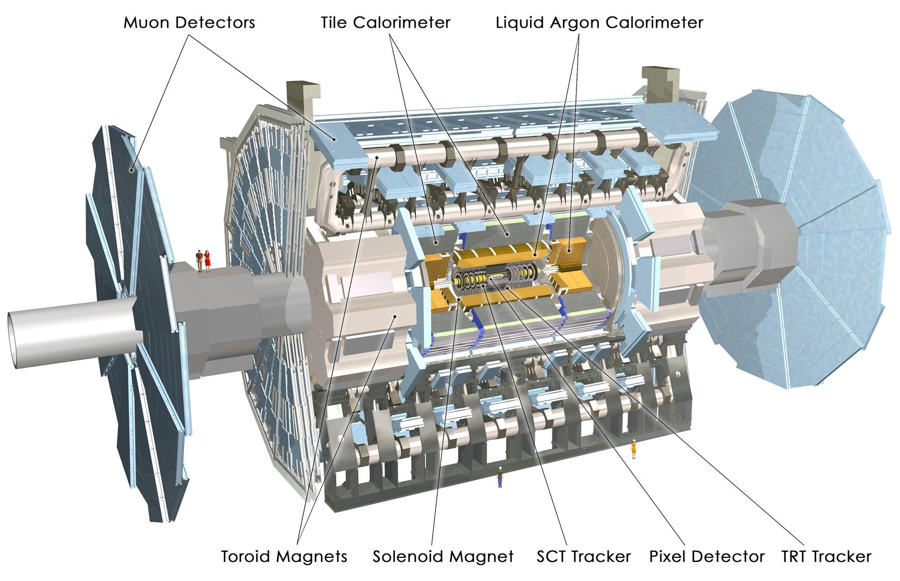
\includegraphics[width=0.75\textwidth, angle=0]{figures/ATLAS_detector_alles_mittel_EN.PNG}
\caption{ The ATLAS detector. Pixel, SCT, and TRT Detectors form the inner detector.  (Taken from \cite{biblio:JINST}) \label{LHC:fig:ATLASDet}}
%\end{center}
\end{figure}

\indent The inner tracker detector is located closest to the collision beam and tracks the path of charged particles such as electrons, and muons. The inner detector will be covered in further detail in section \ref{LHC:ID}. The electromagnetic calorimeter (EM calorimeter) surrounds the inner detector and measures the amount of energy of electromagnetic particles such as electrons and photons. The hadronic calorimeter surrounds the electromagnetic calorimeter and measures the amount of energy of hadrons such as protons and neutrons. The calorimeters are described in further detail in section \ref{LHC:Calorimeter}. The muon spectrometer forms the large outer layer of the detector, surrounding the hadronic calorimeter. Few particles other than muons and neutrinos can penetrate through the calorimeters. The muon spectrometer records the tracks left by the charged muons. The muon spectrometer is described in further detail in section \ref{LHC:MuonSpec}. Neutrinos are undetectable and must be inferred through conservation of momentum. A diagram of the signature left by each particle type is given in figure \ref{LHC:fig:ATLASParticleDiagram} ~\\
\begin{figure}[h!]
%\begin{center}
\centering
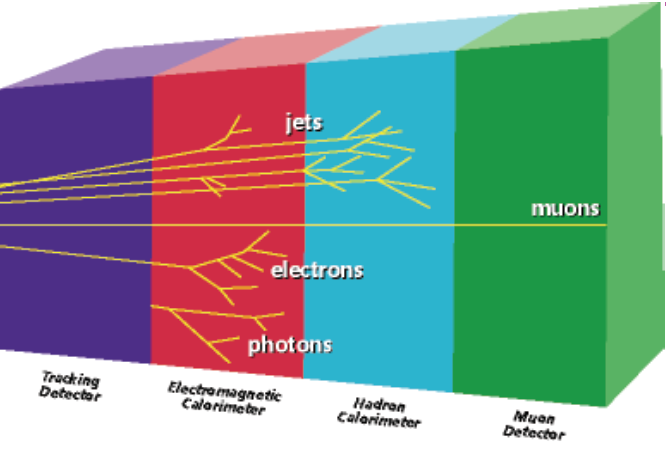
\includegraphics[width=0.55\textwidth, , angle=0]{figures/ATLAS_Particle_Diagram.PNG}
\caption{ The signature left by different particles. (Taken from \cite{biblio:SMcourse}) \label{LHC:fig:ATLASParticleDiagram}}
%\end{center}
\end{figure}

\indent A photon is not charged and so leaves no track. Photons do interact electromagnetically and therefore deposit all their energy in the EM calorimeter in the form of a cascading shower of electrons and photons. Electrons are charged and do leave a track in the inner detector and deposit their energy in the EM calorimeter. Pions and protons are charged and will leave a track in the inner detector, and they will deposit all their energy in the hadronic calorimeter. Neutrons are not charged and will not leave a track. Like protons, neutrons will deposit their energy in the hadronic calorimeter. Muons penetrate the detector and are charged. They will leave a track in both the inner detector and the muon spectrometer. ~\\
\indent Almost all particles that the ATLAS detector is looking for are unstable, meaning the particles will decay before they reach the detector. The final decay product is almost always a combination of the above particles and the undetectable neutrino. The original particle's kinematics is then calculated from the kinematics of each of its measurable decay products. ~\\
\indent Aproximately1000 particles are produced from the collision point every 75 nanoseconds at the Large Hadron Collider.\cite{biblio:JINST} The ATLAS Detector uses a system of triggers to filter this vast amount of data, recording only interesting collisions. The triggering system is complex and depends on the type of particle that is triggered on. This analysis uses the muon triggering system which is described in more detail in section \ref{LHC:MuonTrigger}. ~\\
\indent The ATLAS detector has two equivalent coordinate systems. The rectangular coordinate system x, y, z is defined as follows. The z direction points in the direction of the beam pipe. The positive x direction points to the center of the LHC ring. The positive y direction points in the upward direction. The origin is defined as the center of the ATLAS detector and lie on the center line of the beam pipe. Alternatively, Radius R is defined as the distance from the z axis (also the beam axis). The azimuthal angle $\phi$ is measured around the beam axis, and the polar angle $\theta$ is the angle from the beam axis. Frequently, the pseudorapidity, defined as $\eta =$ - ln~tan$({\theta}/2)$, is used in place of $\theta$ as the third coordinate. ~\\
\subsection{The Inner Detector}
\label{LHC:ID}
\indent The inner detector surrounds the collider beam tube and tracks the path of charged particles including electrons, charged pions, protons, and muons. Figure \ref{LHC:fig:ATLASID} shows the configuration of the inner detector. ~\\
\begin{figure}[h!]
%\begin{center}
\centering
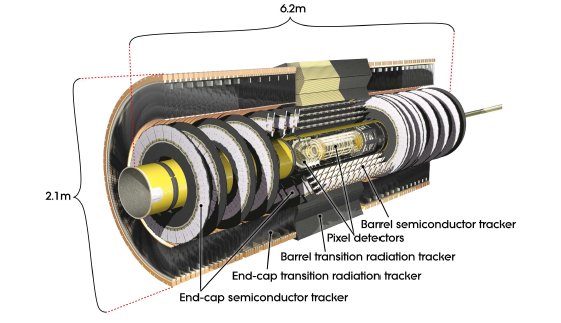
\includegraphics[width=0.75\textwidth, angle=0]{figures/ATLAS_ID_Detector.PNG}
\caption{ Cutaway view of the ATLAS inner detector.  (Taken from \cite{biblio:JINST}) \label{LHC:fig:ATLASID}}
%\end{center}
\end{figure}

\indent The inner detector consists of two silicon semiconductor detectors; the Pixel detector and the Semiconductor Tracker (SCT) and a straw tracker called the Transition Radiation Tracker (TRT). The three detectors operate independently of one another but the information they gather is combined during reconstruction to form a complete track of the particle as it flies through the inner detector. The whole inner detector is immersed in a 2 T magnetic field produced by a solenoidal superconducting magnet that radially surrounds the whole inner detector. At this radii, around 1000 particles will emerge from the collision point every 75 ns demanding that the inner detector have good position and time resolution. \cite{biblio:JINST} ~\\ 
\indent The Pixel detector lies closest to the beam pipe. The Pixel detector uses thousands of pixels of doped silicon that form diodes. The diodes are placed in reverse bias within the larger electronic circuit. Hence no current will flow through the circuit unless the diode breaks down. As a charged particle pass through the diode, they cause small ionizations that momentarily breaks down the diode, allowing current to flow. This current can then be detected and measured. ~\\
\indent The Pixel detector has three layers of pixel sensors in the cylindrical barrel and three wheels of pixel sensors in the endcaps covers a total $|\eta|$ of 2.5. The pixels measures both the $\phi$ and Z coordinate of the hit simultaneously, achieving 10 ${\mu}m$ accuracy in the (R - $\phi$) direction and 115 ${\mu}m$ in the Z direction in the barrel and 10 ${\mu}m$ resolution in the (R - $\phi$) direction and 115 ${\mu}m$ in the R direction in the endcap. \cite{biblio:JINST} ~\\
\indent At larger radii, the SCT surrounds the Pixel detector. The SCT operates in a similar fashion to the Pixel detector as the SCT is also a silicon detector. Instead of pixels of doped silicon, the SCT uses narrow strips of doped silicon. Narrow strips allow measurement of only one coordinate (either the $\phi$ or Z and not both like the Pixel Detectors) per strip but is more cost effective. To compensate for this, the SCT use two orthogonally oriented strips glued back to back to measure both coordinates. The SCT has four planes of these double strips in the cylindrical barrel and four wheels in the endcaps. The SCT can achieve position accuracies of 17 ${\mu}m$ in the (R-$\phi$) direction and 580 ${\mu}m$ in the Z direction in the barrel and 17 ${\mu}m$ in the (R-$\phi$) direction and 580 ${\mu}m$ in the R direction in the endcap. \cite{biblio:JINST} ~\\
\indent The TRT lies at a larger radii around both the SCT and the Pixel detector and covers an |$\eta$| range of 2.0. Unlike the two silicon detectors, the TRT is a straw tracker and is filled with around 300 thousand wire straws. The straws is filled with a combination of xenon, $CO_2$, and $O_2$ gas. As a charged particle flies through the straw, it ionizes that gas within the straw. Voltage is applied to the wall of the straw and the central wire making the straw a capacitor. The positive gas ions and negative free electrons will follow the electric field lines of the capacitor and drift in opposite directions to the central wire and straw wall. The speed of the electron drift is known and based on the timing of the arrival of the first election and the last election, the distance from the center of the straw to the flight path of the charged particle can be determined. This allows the measurement of one coordinate of the particle's flight. This process is shown in figure \ref{LHC:fig:StrawTube}. \cite{biblio:JINST} ~\\
\begin{figure}[h!]
%\begin{center}
\centering
%\includegraphics[width=0.5\textwidth]{plots/ATLAS_Staw_Tube_Fig.pdf}
\includegraphics[width=0.3\textwidth]{figures/ATLAS_Staw_Tube_Fig.PNG}
\\
\caption{ Cross-section of a straw tube with an interacting muon. (Taken from\cite{biblio:JINST}) \label{LHC:fig:StrawTube}}
%\end{center}
\end{figure}

\indent The TRT's straws in the barrel and endcaps are arranged to measure the $\phi$ coordinate of the passing charged particle. The $\phi$ direction is the direction in which charged particles bend. Therefore, the TRT helps to measure the momentum of the charged particle. The TRT provides (R-$\phi$) direction information with an intrinsic accuracy of 130 mm per straw. This large resolution uncertainty is compensated by the large number of hits which a particle leaves in the TRT (around 36 hits per track is expected compared to 8 in the SCT and 3 in the Pixel). ~\\
\indent The TRT also aids in electron identification. The space between the straws is filled with materials with different indexes of refraction. When ultra-relativistic charged particles crosses the boundaries of different materials, they produce transition radiation. The transition radiation will in turn further ionize the gas in the straw, producing a high threshold hit in the straw. Particles with small invariant masses such as electrons are more likely to emit transition radiation. This allows for another form of electron identification and complements the electron identification function of the calorimeter. ~\\
\indent The hits in all three detectors are reconstructed into a track of the flight path of the charged particle by ATLAS reconstruction software. Depending on the curvature of the track, the momentum and charge of the particle can be measured. By matching the track to other signals in the calorimeter or the muon spectrometer, the identity of the charged particle can be determined. ~\\
\subsection{The Calorimeter}
\label{LHC:Calorimeter}
\indent The calorimeter is separated into two types. The electromagnetic calorimeter (EM calorimeter) is designed to measure the energy of electromagnetic particles such as electrons and photons, and the hadronic calorimeter is designed to measure the energy of hadrons such as protons, neutrons, and pions. The calorimeter covers up to an $\eta$ range of $|\eta| < 4.9$. The calorimeter is not only used to measure the energy of jets and particles but also used to reduce the probability of a non-muon particle from punching through to the outer muon detectors. Therefore the total thickness of the EM calorimeter is greater than 22 radiation lengths ($X_0$) in the barrel and greater than 24 $X_0$ in the end-caps.\cite{biblio:JINST} The cut away view of the whole calorimeter is show in figure \ref{LHC:fig:ATLASCalo} ~\\
\begin{figure}[h!]
%\begin{center}
\centering
\includegraphics[width=0.75\textwidth, angle=0]{figures/ATLAS_Calo.PNG}
\caption{ The ATLAS calorimeter. (Taken from \cite{biblio:JINST}) \label{LHC:fig:ATLASCalo}}
%\end{center}
\end{figure}

\indent The inner most calorimeter is the liquid argon electromagnetic calorimeter (EM Calorimeter). The EM calorimeters are made of multiple planes of 1.5 mm thick lead plates. The 4 mm gap between the lead plates is filled with liquid argon. When high energy electrons or photons hit the lead plates they produce more electron-positron pairs through pair production. These newly produced electrons and positrons then will also produce more photons as they fly through the lead plates. This results in a shower of electrons and positrons until the photons no longer have enough energy to pair-produce. When the charged particles traverse the liquid argon, they ionize the argon. These ions and free electrons in the liquid argon drift to external electric terminals and are sensed as a current. The more energetic the initial electron or photon, the more electron - positron pairs will be produced causing a greater ionization in the liquid argon. Also, the more energetic the initial electron or photon, the deeper the electron shower will penetrate the calorimeter before it runs out of energy to produce more electron - positron pairs. Both are used to measure the total energy of the initial electromagnetic particle. The barrel part of the electromagnetic calorimeter covers up to an $|\eta| < 1.475$ and the two endcaps covers the $\eta$ range of $1.375 < |\eta| < 3.2$. ~\\
\indent Outside the electromagnetic calorimeter lie the hadronic calorimeter. The hadronic calorimeter is formed by three different detectors, the barrel tile calorimeter, the hadronic endcap calorimeter (HEC) and the forward hadron calorimeter (FCal). The barrel tile calorimeter covers an $\eta$ range $|\eta| < 1.0$ and two extended barrel tile calorimeter covers $0.8 < |\eta| < 1.7$. The tile calorimeter consists of multiple steel plates with scintillating tiles sandwiched in between. When hadrons such as protons, neutrons, pions, and kaons pass, they interact with the nuclei in the steel via the strong force and produce more hadrons. Those hadrons in turn interact with more steel nuclei eventually producing a shower of hadronic particles. As the hadrons pass the scintillating tiles, they cause the tiles to produce light that is amplified by a photomultiplier tube and then detected. The more energetic the initial hadron, the more hadrons produced in the hadronic shower and the more light is produced in the tiles. Also the more energetic the initial hadron, the deeper the hadronic shower penetrates before the hadrons no longer have enough energy to produce more hadrons. The HEC and the FCAL extends the $\eta$ coverage of the hadronic calorimeter to an |$\eta$| of 4.9. Both are liquid argon calorimeters and operate in the same way as the EM calorimeter. The HEC uses copper instead of lead plates because copper is better at interacting with hadrons than lead. For the same reason, the FCAL uses copper-tungsten plates in place of lead.~\\
\subsection{The Muon Spectrometer}
\label{LHC:MuonSpec}
\indent The muon spectrometer tracks muons with high enough energy to penetrate the calorimeter. Few particles other than muons and the undetectable neutrino can penetrate the large calorimeter. The muon spectrometer consist of two precision tracking detectors, the Monitored Drift Tube (MDT) and the Cathode Strip Chamber (CSC), and two detectors used in muon triggering, the Resistative Plate Chambers (RPC) and the Thin Gap Chambers (TGC). The muon triggering system is discussed in more detail in \ref{LHC:MuonTrigger}. The configuration of the muon system is shown in figure \ref{LHC:fig:ATLASMuonSpec} ~\\
\begin{figure}[h!]
%\begin{center}
\centering
\includegraphics[width=0.75\textwidth, angle=0]{figures/ATLAS_MuonSpec.PNG}
\caption{ Cutaway view of the ATLAS Muon Spectrometer. (Taken from \cite{biblio:JINST}) \label{LHC:fig:ATLASMuonSpec}}
%\end{center}
\end{figure}

\indent The muon spectrometer is immersed in a magnetic field produced by eight superconducting toroid magnets in the barrel and eight superconducting toroid magnets in the endcaps. The barrel magnets cover an |$\eta$| range of 1.4 and the endcap magnets cover an |$\eta$| range from 1.6 to 2.7. The area with $1.4 < |\eta| < 1.6$ is called the transition region with a mixed magnetic field from both the barrel and endcap. The endcap magnets are offset from the barrel magnets by 22.5 degrees in the $\phi$ direction to allow a smoother magnetic field in this region. The configuration of the magnets is shown in figure \ref{LHC:fig:ATLASMag} ~\\
\begin{figure}[h!]
%\begin{center}
\centering
\includegraphics[width=0.60\textwidth, angle=270]{figures/ATLAS_ToroidMag.PNG}
\caption{ Geometry of the barrel and endcap toroid magnets. The cylinder repesents the calorimeter. (Taken from \cite{biblio:JINST}) \label{LHC:fig:ATLASMag}}
%\end{center}
\end{figure}

\indent The magnetic field bends the charged muons in the $\eta$ direction. The bending power of the magnets depends on the direction of muon travel. In the pseudorapidity range $0 < |\eta|< 1.4$, the barrel toroid provides 1.5 to 5.5 Tm of bending power. In between $1.6 < |\eta| < 2.7$, the end-cap toroids provide approximately 1 to 7.5 Tm of bending power. The bending power is lower in the transition region. ~\\
\indent The path of the muon can be reconstructed and the momentum of the muon can be measured from the amount of bending. The size of the muon spectrometer combined with the inner detector allows ATLAS to track muons over long distances. This is important because longer tracks mean more precise momentum measurements.\cite{biblio:JINST} ~\\
\indent The Monitored Drift Tube (MDT) consists of three to eight layers of drift tubes and covers an $\eta$ range of |$\eta$| < 2.7. The inner-most layer of the MDT only covers up to an $\eta$ range of |$\eta$| < 2.0. In the $\eta$ range between $2.0 < |\eta| < 2.7$, the Cathode Strip Chamber (CSC) replaces the MDT inner layer. ~\\
\indent The drift tubes of the MDT functions in the same manner as the straw tubes of the TRT in the inner detector. The muon ionizes the gas inside the tube and frees electrons. These electrons drift to the central wire of the drift tube because of the voltage difference between the central wire and the tube wall. The arrival of the electrons creates a pulse of current that is registered as a hit. How drift tubes operate is discussed in more detail in section \ref{LHC:ID}. The purpose of the MDT is to precisely measure the coordinates of the muon flight path in the bending $\eta$ direction. This measurement of the bending coordinate is used in the calculation of the momentum of the muon. The resolution of the MDT is 80 $\mu$m per tube.\cite{biblio:JINST}~\\
\indent The CSC replaces the inner MDT layer in the forward $\eta$ ranges between 2.0 and 2.7. This is needed because in this section the expected density of muons exceeds the safe operational limits of the MDT.\cite{biblio:JINST} The CSC is formed with multiwire proportional chambers. The chambers are formed with strips of cathode capacitor plates on either side and a row of anode wires sandwiched in between. As a charged particle flies through the chamber it will ionize the gas in the chamber, freeing electrons and positively charged ions. The free electron will drift along electric field lines to the nearest wire and the ions will drift to the cathode plates strips. Different electrons may end up in different wires as the ionization area has some spread and different ions on different strips. The CSC then regresses the position of the muon from the proportions of signal in each strip. The structure of the CSC is show in figure \ref{LHC:fig:ATLASCSC}. ~\\
\begin{figure}[h!]
%\begin{center}
\centering
\includegraphics[width=0.50\textwidth, angle=0]{figures/ATLAS_CSC.PNG}
\caption{ Diagram of a plane in the ATLAS Cathode Strip Chamber. (Taken from \cite{biblio:JINST}) \label{LHC:fig:ATLASCSC}}
%\end{center}
\end{figure}

\indent The wires are arranged in the radial direction. This allows the wires to measure the $\phi$ coordinate of the muon. On one side, the cathode strips are arranged parallel to the wire to complement the measured $\phi$ coordinate of the muon and to reduce noise levels. On the other side, the cathode strips are arranged transverse to the wires to measure the $\eta$ coordinate of the muon. The resolution achieved by the CSC is 40 $\mu$m in the bending $\eta$ plane and about 5mm in the transverse$\phi$ plane. The difference is because the $\eta$ coordinate is measured by the cathode strips and the $\phi$ coordinate is measured by the wires. \cite{biblio:JINST} ~\\
\indent The RPC and TGC are trigger chambers with the goal of quickly measuring the position of the muon. The RPC chamber is formed by two orthogonal planes of cathode and anode strips. The gas in between the planes is chosen such that the gas sparks when a muon passes through. The sparking allow near-instantaneous detection of muons instead of waiting for the electrons and ions to drift onto the plates. The two orthogonal planes measure both the $\eta$ and $\phi$ coordinates of the muon track. The RPC extends out to an $|\eta|$ of 1.05 and covers the barrel of the detector. The TGC is a multiwire proportional chambers and operates similarly to the CSC. The TGC covers the $|\eta|$ range between 1.05 and 2.7 and covers the endcaps of the detector. However, the TGC can only trigger up to an $|\eta|$ of 2.4. The trigger system and software is described in section \ref{LHC:MuonTrigger}. ~\\
\indent The MDT can only measure the $\eta$ coordinate and not the $\phi$ coordinate of the muon. To compensate for this, the MDT chamber hits are matched to the respective RPC or TGC chamber hits and uses the $\phi$ coordinate of the trigger chamber as the second coordinate of the hit. If more than one muon passes through an MDT and trigger chamber pair then there is no unambiguous method to match the hits. Therefore the muon density in the MDT chambers must be low. Fortunately, simulations show that the number of muons that reach the muon spectrometer with $P_T > 6$ GeV is about $6*10^{-3}$ per beam-crossing, corresponding to about $1.5*10^{-5}$ per chamber.\cite{biblio:JINST} Assuming uncorrelated tracks, the probability of finding more than one track in any MDT/trigger chamber pair is very small. \cite{biblio:JINST} If two muons do traverse the same chamber, then the corresponding inner detector tracks of the muons are used to resolve the ambiguity. ~\\
\indent The hits recorded by the muon spectrometer detectors are reconstructed into the track of the flight path of the muon. The muon track is then matched to the inner detector track of the muon by the ATLAS reconstruction software MuID and STACO. This forms one complete combined muon track that traverses the whole ATLAS detector. The uncertainty of the momentum measurement is inversely related with the length of the track. Therefore, the long length the combined muon track serves to give precise measurements of the momentum of the muon. ~\\
\subsection{The Muon Trigger System}
\label{LHC:MuonTrigger}
\indent The ATLAS triggering system consists of three levels of triggers. At each level, more information is acquired for the event and the trigger refines the decision on whether the event is interesting. Because interesting events corresponds to high energy particles, the muon trigger selects high transverse momentum ($P_T$) muons. The first level trigger (L1 trigger) makes a decision in less than 2.5 ${\mu}s$ and reduces the rate of data collection to 75 kHz.\cite{biblio:JINST} The two higher level triggers, the Level 2 trigger (L2 trigger) and the event filter, further reduces the data recording rate to 200 Hz. \cite{biblio:JINST} ~\\
\indent For muons, the ATLAS L1 trigger depends on information gathered by the Resistive Plate Chambers (RPC) and the Thin Gap Chambers (TGC) detectors to quickly estimate the muon's $P_T$. ~\\
\indent The L1 RPC trigger compares the hit pattern of the measured muon to the theoretical infinite momentum muon to estimate the $P_T$ of the muon. The trigger electronics draws a line from the collision point to the hit in the middle 'pivot' layer of the RPC. If the muon has high transverse momentum we would expect a hit in both the inner and outer layer of the detector that are close to being on a straight line from the origin. If the transverse momentum of the muon is low then we would expect a hit that is far from a straight line in the inner layer and either a far away hit or no hit in the outer layer. The distance of the hits from the theoretical straight line is used to quickly estimate the $P_T$ of the muon without reconstructing the track of the muon. For the TGC detector, the pivot layer is the outer layer due to the positioning of the endcap magnets. This process is show schematically in figure \ref{LHC:fig:RPCTriggerAlg}. ~\\
\begin{figure}[h!]
%\begin{center}
\centering
\includegraphics[width=0.70\textwidth, angle=0]{figures/l1_algo.PNG}
\caption{ The Level 1 Trigger Algorithm used to estimate the $P_T$ of muons using the RPC and TGC Detector. (Taken from \cite{biblio:TriggerTwiki}) \label{LHC:fig:RPCTriggerAlg}}
%\end{center}
\end{figure}

\indent The L2 algorithm reconstructs the tracks of the muons which pass the L1 Trigger and get a more precise measurement of the muon $P_T$. With this information, the L2 trigger refines the decision on whether to keep the event. The rate of events which pass the L2 trigger is reduced to around 2 kHz. If the event passes the L2 trigger, the event filter (EF) reconstructs combined muons, calorimeter measurements, and vertices with more precise software. The EF software reduces the rate of events that will be fully reconstructed offline to a manageable 200 Hz. The trigger system is summarized in figure \ref{LHC:fig:MuonTrigFlow}. ~\\
\begin{figure}[h!]
%\begin{center}
\centering
\includegraphics[width=0.70\textwidth, angle=270]{plots/SchemaMuonTriggerSlice.pdf}
\caption{ Flow chart of the muon trigger system. (Taken from \cite{biblio:TriggerTwiki}) \label{LHC:fig:MuonTrigFlow}}
%\end{center}
\end{figure}


\chapter{Object Reconstruction at ATLAS}
\label{chap:reconstruction}

\section{Inner Detector Track Reconstruction}
\label{sec:reco:IDtrack}

\indent  Many reconstructed physics objects depend on tracking information in the inner detector (ID).  ID tracks are combined with the EM calorimeter and muon spectrometer information to identify and measure the momentum of electrons and muons.  Hadronic jets use ID tracks to determine if the jet originated from a heavy flavored hadron containing b-quarks or only light flavored hadrons.  ID tracks are also crucial to identifying whether objects originate from the interesting hard scattering interaction or a less interesting pile-up interaction.\\

\indent Two types of inner detector tracks are reconstructed, primary tracks and secondary tracks.  Primary tracks originate from the interaction point (IP) and are meant to reconstruct the trajectories of charged particles originating directly from the proton-proton collisions.  Secondary tracks target charged particles originating in the ID from secondary decays and interactions such as $\gamma \rightarrow e^{+}e^{-}$ conversions.  \\

\indent Primary tracks are reconstructed using the {\tt NEWT} algorithm.  The {\tt NEWT} algorithm starts from seed segments in the inner silicon detectors and extended outwards towards the TRT. Greater details can be found in reference [\cite{NEWT}]. A brief summary of the track reconstruction algorithm will be given here.\\ 

\indent First, seed segments are created from three space point measurements in silicon detectors.  Each pixel cluster corresponds to a single space point measurement since a single pixel sensor provides 3D position information.  Two SCT clusters from the same SCT layer must be combined to form a single space point measurement because each SCT strip only provides 2D position information.  \\

\indent Seed segments can be formed out of all pixel (PPP), all SCT (SSS) or two pixel and one SCT (PPS) space points.  PSS space points are rejected due to high fake rates.  \\

\indent Starting from the original seed segment, track reconstruction is extrapolated layer by layer through the inner detector. Hits are added to the track one layer at a time.  If multiple tracks share a hit, then the shared hit is assigned to the most precise track.  \\%If multiple charged particles are close together when they traverse a pixel layer, they can form merged clusters in the Pixel detector.  These merged pixel clusters are split using a set of trained neural networks. \\

\indent In contrast, secondary tracks are reconstructed from the TRT and extrapolated inwards towards the direction of the beam line.  Segments are reconstructed in the TRT and then extended inwards by adding silicon hits. \\

\section{Vertex Reconstruction}
\label{sec:reco:vtx}

\indent On average around 25 proton-proton interactions occur in every beam crossing in Run 2.  These p-p interactions are spread out in the $Z$ coordinate due to the finite bunch length at the LHC.  We are able to reconstruct the original interaction vertex (primary vertex) by tracing back charged particle tracks to the beam line.  We are able to differentiate objects from the interesting hard scattering p-p interaction from other pileup interactions using reconstructed vertexes.  A summary of the primary vertex reconstruction algorithm is given in this section.  \\

\indent A subset of reconstructed ID tracks are used to reconstruct the primary vertexes.  In Run 2 tracks must satisfy:

\begin{itemize}
\item[] $\pt > 400 \mev$
\item[] $|\eta| < 2.5$
\item[] number of silicon hits $ \ge 9$ if $|\eta| \le 1.65$ or $\ge 11$ if $|\eta| > 1.65$
\item[] IBL hits + B Layer hits $\ge 1$
\item[] maximum $1$ shared module ($1$ shared pixel hit or $2$ shared SCT hit)
\item[] pixel holes $= 0$
\item[] SCT holes $\le 1$
\end{itemize}

\indent A vertex seed is found by searching for the global maximum in the $Z$ coordinate of reconstructed tracks.  The vertex position is fitted using an algorithm that is robust to additional noise and outlier tracks called the adaptive vertex fitting algorithm \cite{VertexReco,adaptiveFitting}.  \\

\indent Adaptive fitting determines the vertex position using a least squared fitting method, but gives the outlier tracks lower weights in the fit.  The vertex position is repeatedly fitted until the fit position no longer changes. A new vertex center is found and new set of weights is calculated for each new fit.  The weighting function also changes from fit to fit according to a predeterminate way; giving more weight to a smaller sub-set of tracks each iteration, ultimately approaching a step function.  \\%The final set of tracks selected is fitted to determine the final position and uncertainty of the vertex. \\

\indent This method of lowering the weight of outlier tracks in each fit and decreasing the weight in each iteration is called determinist annealing. \cite{adaptiveFitting}  The procedure is analogous to repeatedly heating and cooling metal in a forge to make the metal's crystal lattice more regular.  At each iteration, a more compact and regular set of tracks are selected eventually ending in a fix set of selected tracks.  \\

\indent  After determining the vertex position, all tracks within $7\sigma$ of the vertex is considered to be associated with the vertex.  A conservative $7\sigma$ acceptance is used to avoid one energetic vertex being split into two during reconstruction.  Tracks incompatible with the vertex from a new vertex seed.  This process is repeated until all tracks have been clustered into vertexes or no additional vertexes can be found.  Each vertex must have at least two associated tracks. \\

\indent The primary vertex with the highest total $\pt$ summed over all associated tracks is identified as the vertex of the hard scattering interaction.  All other primary vertexes are referred to as pileup vertexes.


\section{Hadronic Jets}
\label{sec:reco:jets}

\indent Energetic partons carrying color charge produced in the initial hard scattering will quickly fragment into multiple hadrons.  The result is a shower of charged and neutral hadrons referred to as a parton shower.  The parton shower leaves a roughly conical energy deposit in the electromagnetic and hadronic calorimeter and multiple associated tracks in the inner tracker.  Some energy may even be deposited in the muon spectrometer if the initial hadron is energetic enough.  This detector signature is referred to as a jet. \\

\indent Identification and reconstruction of hadronic jets is very important for many different detector signatures including this analysis.  Of key importance is the correct reconstruction of the initial parton energy.  Also important is the rejection of jets resulting from pile-up interactions and identifying jets resulting from b-quarks.  Jet reconstruction and energy calibration are described in sections \ref{sec:jet:reco} and \ref{sec:jet:calib}.  Jet vertex tagging and b-jet tagging are described in section \ref{sec:jet:JVT} and \ref{sec:jet:btag}.

\subsection{Hadronic Jet Reconstruction}
\label{sec:jet:reco}

\indent Hadronic jets are reconstructed by clustering energy deposits in the calorimeter. First, all topologically connected calorimeter cells are clustered around a seed cell that passes the $4\sigma$ signal above noise threshold.  These 3D clusters are referred to as topological clusters (topo-clusters).\cite{jetReco7TeV,jetReco13TeV}  Neighboring cells around the cluster are added to the cluster if they pass a $2\sigma$ signal over noise threshold. This step is repeated until no neighboring cells pass the $2\sigma$ signal over noise threshold.  At this stage, one last round of neighboring cells is added regardless of the amount of signal to noise ratio in those cells. \\

\indent Topo-clusters are then grouped into jets according to the $\antikt$ algorithm.  The $\antikt$ algorithm groups objects according to the distance measure $d_{ij}$ defined in equation \ref{eqn:antikt} with parameter $p=-1$.  All objects within $d_{ij}$ less then $d_{iB}=k^{2p}_{Ti}$ are grouped into a single jet.  \\

\begin{equation}
d_{ij} = min ( k^{2p}_{Ti}, k^{2p}_{Tj} ) \frac{(\Delta\eta^2_{ij} + \Delta\phi^2_{ij})}{R^2}
\label{eqn:PileupDensity}
\end{equation}

\indent  The algorithm can best be explained by examining an example case.  If a hard object $1$ exists and is surrounded by only soft objects $j$ then $d_{1j}$ equals $k^{2p}_{1j}(\frac{\Delta R^2}{R^2})$ for all $j$ where $\Delta R = \Delta \eta^2 + \Delta \phi^2$.  $d_{1j}$ will always be less then any $d_{ij}$ if both $i$ and $j$ are both soft and have the same $\Delta R$ as $1$ and $j$.  Therefore, the $\antikt$ algorithm effectively groups hard objects first before soft objects.  \\

\indent A perfectly conical jet of radius $R$ will be formed if no other hard objects are found within a cone of $2R$.  If two hard objects exist within $R<\Delta R_{1,2}<2R$ of one another then two jets will be formed splitting the energy cells between them.  If two hard objects exist within $\Delta R_{1,2}<R$ then they will both be grouped into a single jet. \\

\indent  The $\antikt$ algorithm is both infrared and collinear safe.  Meaning the algorithm is insensitive to the radiation of additional soft particles and the collinear splitting of initial partons.  Additional soft partons do not change the shape of the jets but the jet shape is flexible to accommodate the presence of other hard radiation. \\

\indent ID Tracks are associated with jets according to a ghost association procedure.\cite{JetAreaGhostAssociate}  Tracks with the same direction and location as real ID tracks but infinitesimally low $\pt$ are allowed to be clustered by the $\antikt$ algorithm.  If these tracks are assigned to the jet by the $\antikt$ algorithm then the real track is associated with the jet.  In this way, we can determine which tracks are associated with the jet without disturbing the clustering of calorimeter energy.  The same procedure of clustering infinitesimally low $\pt$ objects is used to determine the jet area. \\

\subsection{Jet Calibration and Systematics}
\label{sec:jet:calib}

\indent Both the electromagnetic and hadronic calorimeters at ATLAS are sampling calorimeters.  The energy deposited in the absorber material is effectively lost because the absorber do not actively record a signal.  Therefore the energy measured using the active material must be scaled up to compensate for this loss.  For this reason and others including leakage of energy outside of the calorimeter edges and deposition of energy below the energy thresholds, reconstructed jets must be calibrated to determine the original hadron's energy.  \\

\indent  A variety of MC based and data based methods are used to calibrate hadronic jets.  Figure \ref{fig:jetCalibFlow} shows the steps in jet calibration for Run 2.\cite{Calibartion13TeV} \\

\begin{figure}[htb]
  \begin{center}
    \includegraphics[width=0.85\textwidth]{figures/JetCalib/JetCalibFlow.png}\hspace{0.05\textwidth}
\end{center}
\caption{Flow chart of the steps involved in jet calibration. (Figure taken from \cite{Calibartion13TeV}) }
\label{fig:jetCalibFlow} 
\end{figure}

\indent First the individual topo-clusters in the jet are calibrated to the energy scale of EM showers using MC simulations.\cite{topoCalib}  It should be noted that this calibration is to EM showers correctly calibrates the energy in EM showers but underestimates the amount of energy lost in hadronic showers.  Additional corrections are applied in the following steps to account for this difference. \\
% The origin of the reconstructed jet is also set to the primary vertex instead of the default detector center. \\

\indent A correction for energy deposited by pileup interactions are applied.\cite{pileupsub}  The correction is based on the measurement of average energy originating from pileup $\rho$ multiplied by the measured jet area.  The pileup energy density is defined in equation \ref{eqn:PileupDensity} and determined by measuring the median energy density of $R=0.4$ $k_t$ jets found in the central $|\eta|<2.0$ part of the calorimeter.  The $k_t$ algorithm preferentially cluster soft objects first instead of hard objects and is more sensitive to soft pileup radiation and no $\pt$ thresholds are applied to the reconstructed $k_t$ jets as we are trying to measure soft objects.  \\

\begin{equation}
\rho=median\{ \frac{p_{T i}^{k_t~jet}}{A_i^{k_t~jet}} \}
\label{eqn:PileupDensity}
\end{equation}

\indent The area based pileup energy correction is subtracted along with two other residual corrections.  The total pileup correction to jet $\pt$ is given in equation \ref{pilupCorrection}. \\

\begin{equation}
p_T^{corr} = p_T - \rho \times A - \alpha~\times (N_{PV} - 1 ) - \beta~\times <\mu>
\label{eqn:pilupCorrection}
\end{equation}

\indent  It should be noted that the jet energy response still has a dependence on pileup after this area based correction has been applied.  The sources of this dependence can be attributed to the incomplete cancelation of in-time and out-of-time pileup.\cite{JetCalibartion13TeV}  For example, events with a low number of reconstructed vertexes ($N_{PV}$) in a run with high average number of interactions per bunch crossing ($<\mu>$) may receive relatively large amounts of out-of-time pileup compared to in-time pileup.  This effect is also parameterized by using the constants $\alpha$ and $\beta$ in equation \ref{pilupCorrection}. \\  

\indent In the next step, the jet energy scale (JES) is applied.  JES is a scale factor which relates the reconstructed jet energy with the true jet energy.  JES is calibrated using a number of MC and data driven methods.  The JES is derived from an inclusive jet MC after pileup and origin corrections have been applied.  \\

\indent A residual difference between the energy responses of gluon and light quark jets remains after JES calibration.\cite{JetCalibartion13TeV}  The difference can be as large as 8 percent and is due to a number of reasons including the factor of 2 difference in color charge between quarks and gluons.  A global sequential correction scheme (GSC) is applied to account for this deference and correct for other detector based issues.\cite{jet_GSC}  \\

\indent GSC corrections uses information on the topology of energy deposits, associated inner detector tracks and activity in the muon spectrometer behind the jet.  ID Tracking information is used to reduce the flavour dependence because gluon initiated jets tend to have a wider profile and more tracks. Muon spectrometer information is used to better estimate high energy jets which penetrate the full depth of the calorimeter.  Information on the relative amount of calorimeter energy deposited in specific layers is used to improve the jet energy resolution. \\

\indent Lastly, further corrections to the jet energy response are obtained by measuring the balance between jets and some reference objects directly in data. \cite{JES_ZGamma,JES_dijet}  The reference object can be a photon, a $Z$ boson or other jets.  The $\pt$ balance between jets and the reference objects are measured in data and compared to the MC.  A residual correction is applied by the data over MC ratio based on equation \ref{jet_insitu}.  Systematic uncertainties on the jet energy responses including those on the jet energy scale and jet energy resolution are also derived using these data driven methods. \\

\begin{equation}
\frac{R_{data}}{R_{MC}} = \frac{<p_T^{jet}/p_T^{ref}>_{data}}{<p_T^{jet}/p_T^{ref}>_{MC}}
\label{eqn:jet_insitu}
\end{equation}

\indent The jet $\pt$ resolution for $|\eta|<0.8$ and $0.8<|\eta|<1.2$ jets are shown in figure \ref{fig:jet_ptresolution}.\cite{JES_dijet} \\

\begin{figure}[htb]
  \begin{center}
    \includegraphics[width=0.45\textwidth]{figures/JetCalib/JetCentral_Response.png}\hspace{0.05\textwidth}
    \includegraphics[width=0.45\textwidth]{figures/JetCalib/JetTransition_Response.png}\hspace{0.05\textwidth}
\end{center}
\caption{Jet $\pt$ resolution for $|\eta|<0.8$ and $0.8<|\eta|<1.2$ jets as a function of jet $\pt$ in 8 TeV data. (Figure taken from \cite{JES_dijet}) }
\label{fig:jet_ptresolution} 
\end{figure}

\subsection{Pileup Jet Rejection and Jet Vertex Tagger}
\label{sec:jet:JVT}

\indent It is imperative to be able to distinguish between jets originating from the hard scattering interaction (hard scattering jets) and those originating from other pile-up interactions (pileup jets) in the high luminosity LHC environment.  Pileup jets may originate from both the on average 25 additional p-p interactions in the same bunch crossing or from interactions in other beam crossings.  We distinguish between the hard scattering jets from pileup jets using a multivariate discriminate known as the jet vertex tagger (JVT).\cite{JVT} \\

\indent The JVT discriminate is based on two variables $\corrJVF$ and $\RpT$ defined in equations \ref{eqn:corrJVF} and \ref{eqn:RpT}.

\begin{equation}
\corrJVF = \frac{\sum_i p_T^{trk_i} (PV_0) }{ \sum_l p_T^{trk_l} (PV_0) + \frac{\sum_{n\ge1} \sum_l p_T^{trk_l} (PV_n) }{k\dot n^{PU}_{trk}} }
\label{eqn:JVF}
\end{equation}

\begin{equation}
\RpT = \frac{\sum_i p_T^{trk_i} (PV_0) }{ p_T^{jet} }
\label{eqn:RpT}
\end{equation}

\indent The $\corrJVF$ variable roughly corresponds to the fraction of a jet's ID track $\pt$ that originate from the hard scattering vertex.  $\sum_i p_T^{trk_i} (PV_0)$ is the sum of all jet's associated track $\pt$ that originate from the primary vertex $PV_0$.  The quantity $p^{PU}_T = \sum_{n\ge1} \sum_l p_T^{trk_l} (PV_n)$ is the total amount of a jet's associated track $\pt$ that originates from pile up interactions.  $p^{PU}_T$ is divided by $k\dot n^{PU}_{trk}$ to correct for the fact that $<k\dot n^{PU}_{trk}>$ will increase linearly with the number of pileup vertexes $n^{PU}_{trk}$.  This makes the variable $\corrJVF$ roughly independent to the number of reconstructed vertexes. The value $k$ is set to an arbitrary $0.01$ and the discriminating power of JVT was found to be independent of the choice of $k$.\\

\indent $\RpT$ is defined as the total track $\pt$ of all associated tracks that originate from the primary vertex $PV_0$ divided by the fully calibrated jet $\pt$. It is important to note that the calibrated jet $\pT$ includes pileup subtraction.  $\RpT$ peaks sharply at zero for pileup jets.  On the other hand, $\RpT$ corresponds to roughly the charged $\pt$ fraction in hard scattering jets.  \\

\indent The JVT discriminate constructs a 2D likelihood based on these variables.   The JVT discriminate determines the probability that a jet will be a hard scattering jet using the k-nearest neighbor (kNN) multivariate technique \cite{TMVA} trained on a $20<\pt<50 \gev$ and $|\eta|<2.4$ MC sample of hard scattering and pileup jets.  The k-nearest neighbor (kNN) algorithm is robust relative to local fluctuations in sparsely populated regions.  \\

\indent For our analysis we require a jet vertex tagger value greater than 0.59.  This corresponds to a 92 percent efficiency for jets originating from the hard scattering interaction and a 2 percent fake rate from pileup jets, if the jet has $|\eta| < 2.4$ and $\pt < 60 \gev$.  The JVT efficiency as a function of jet $\pt$ is shown in figure \ref{fig:JVT_eff} \\

\begin{figure}[htb]
  \begin{center}
    \includegraphics[width=0.65\textwidth]{figures/JetCalib/JVT_eff.eps}\hspace{0.05\textwidth}
\end{center}
\caption{The distribution showing the jet vertex tagger efficiency as a function of jet $\pt$ in 2015+2016 data. Only jets balanced against a $Z->\mu\mu$ boson are accepted.  Details can be found in \cite{JVT}. }
\label{fig:JVT_eff} 
\end{figure}

\subsection{Jet Quality and Jet Cleaning}
\label{sec:jet:quality}

\indent Several variables are useful in discriminating between real hadronic jets and fake jets not coming from p-p interactions.  The sources of fake jets include noise in the LAr and Tile calorimeters, beam induced backgrounds and cosmic raw showers.  These variables can be divided into three broad categories: variables quantifying the EM and hadronic calorimeter energy ratio, ID track based variables and variables based on the pulse shape of the LAr calorimeters.  Detailed descriptions of the variables used can be found in \cite{JetCleaning} a brief summary will be given here.\\

\indent Energy ratio variables can reject calorimeter noise and beam induced backgrounds and energy deposited from cosmic rays.  Jets originating from beam induced backgrounds tend to concentrate more energy in a few longitudinal layers compared to jets from p-p collisions.  Multiple variables corresponding to the fraction of jets energy deposition in any one section along the expected direction of the shower relative to the total energy deposition are useful in discriminating against fake jets. \\

\indent Energy ratio variables include: \\

\begin{itemize}
\item[] $f_{EM}$: ratio of EM calorimeter energy to total jet energy
\item[] $f_{HEC}$: ratio of HEC calorimeter energy to total jet energy
\item[] $f_{max}$: maximum energy fraction in any single calorimeter layer
\end{itemize}

\indent ID track based variables are useful because tracks can be matched to the primary vertexes in good jets.  Fake jets have low fraction of tracks which can be matched to primary vertexes.  \\

\indent list of track based variables include: \\

\begin{itemize}
\item[] $f_{ch}$: ratio of the scalar sum of ID track $\pt$ where ID track must originate from the primary vertex to jet $\pt$.  approximately the fraction of jet energy carried by charged particles.  
\item[] $f_{ch}/f_{max}$: ratio of $f_{ch}$ and $f_{max}$, the maximum energy fraction in any single calorimeter layer
\end{itemize}

\indent Pulse shape in the LAr should be consistent with those of a particle shower in good jets.  A quality variable $Q^{LAr}_{cell}$ measures the quadratic difference between expected and actual pulse shapes in each LAr cell.  Quality variables based on the fraction of cells in a jet with poor quality and the average quality is found to provide discrimination power against LAr noise. \\

\indent LAr pulse shape variables include: \\

\begin{itemize}
\item[] $\braket{Q}$: weighted average of pulse quality of LAr cells ($Q^{LAr}_{cell}$) in a jet.  Normalized to $0 < \braket{Q} < 1$.
\item[] $f^{LAr}_{Q}$: Fraction of energy in cells with poor quality pulse shapes in EM LAr Calorimeter
\item[] $f^{HEC}_{Q}$: Fraction of energy in cells with poor quality pulse shapes in hadronic endcap calorimeters (HEC) which also use LAr technology.
\item[] $E_{neg}$: total energy of all cells with negative energy
\end{itemize}

\indent A jet satisfying any one of the following criteria is considered a {\tt BadLoose} jet.  The presence of a {\tt BadLoose} can result in poor $\met$ reconstruction due to a noisy calorimeter or beam induced background.  Therefore, if any baseline jet in the event is found to be {\tt BadLoose} then the entire event is rejected.   This procedure is called jet cleaning.  \\

\indent A jet is considered a {\tt Loose} jet if is not identified as a {\tt BadLoose} jet.  {\tt Loose} jets are used as signal jets in most ATLAS physics analysis including this one. \\

\begin{enumerate}
\item[] $f_{EM} > 0.5$ and $|f^{HEC}_{Q}| > 0.5$ and $\braket{Q} > 0.8$
\item[] $E_{neg} > 60 \gev$
\item[] $f_{EM} > 0.95$ and $f^{LAr}_{Q} > 0.8$ and $\braket{Q}>0.8$ and $|\eta|<2.8$
\item[] $f_{max}>0.99$ and $|\eta|<2.0$
\item[] $f_{EM}<0.05$ and $f_{ch}<0.05$ and $|\eta|<2$
\item[] $f_{EM}<0.05$ and $|\eta|\ge2$
\end{enumerate}

\subsection{Identifying Jets Originating from Heavy Flavor Hadrons}
\label{sec:jet:btagging}

\indent Hadrons containing b-quarks have long lifetimes, around 1.5 ps or a $c\tau$ of roughly 450 $\mu$m.  The long flight distance allows us to reconstruct ID tracks with large impact parameters and perhaps reconstruct secondary vertexes. \\% The typical b-hadron decay consist of at least one vertex displaced from the point of initial hard scattering.  \\

\indent Three separate algorithms have been setup to distinguish jets originating from b-hadrons (b-jets) from light hadrons and c-hadrons (c-jets).  A brief description of each algorithm is given in this section.  More details can be found in \cite{btagging2016}  and \cite{btagging2015}.  \\

\indent The first algorithm is based on track impact parameters for high quality tracks that are associated with jets.  The discriminate is computed as a sum of the log likelihood ratio of each accepted track in the vertex or $\sum_i \ln(\frac{p_b}{p_{light}})$, where i sums over all accepted tracks in the jet and $p_b$ is the PDF for a b-jet and $p_{light}$ is the PDF for a light jet.  The PDF uses transverse and longitudinal impact parameters $d_0$ and $z_0$ as observables and is derived from MC simulation.  \\

\indent The second algorithm seeks to reconstruct the secondary vertex associated with the b-hadron decay.  This algorithm has the advantage that if a secondary vertex is consistent with the decays of long lived hadrons that do not contain b-jets such as $K_s$ or $\Lambda$ or photon conversions then the vertex maybe rejected.  For example, secondary vertexes with a mass greater then $6 \gev$ are inconsistent with b decays and are rejected. Variables based on the secondary vertex location, energy, and mass can all be used to discriminate b-jets from light-jets and c-jets.  \\

\indent The third algorithm attempt to reconstruct the full b-hadron decay chain and is called the decay chain multi-vertex reconstruction algorithm.  The algorithm uses a Kalman filter to determine the common line on which the primary vertex and the bottom/charm vertexes lie.  \\

\indent The output of the three algorithms are all combined into a multivariate discriminate called MV2.  MV2 uses a boosted decision tree (BDT) algorithm \cite{TMVA} to gain better separation power between different jet flavors. This analysis uses the MV20c10 discriminate to tag b-jets. MV20c10 is selected as it gives the best balance between light jets and c-jet rejection for a given b-tagging efficiency.  \\

\indent The b-tagging efficiencies and mis-tag rates have been calibrated by the ATLAS flavor tagging group.  The distribution of the MV20c10 discriminate for light, charm and b-hadrons can be seen in figure \ref{fig:MV20c10}. We make a selection at MV2c10 $ > 0.6459$ which corresponds to approximately 77\% b-tagging efficiency with a factor of 134 reject rate for light jets.  \\

\begin{figure}[htb]
  \begin{center}
    \includegraphics[width=0.85\textwidth]{figures/JetCalib/MV20c10.eps}\hspace{0.05\textwidth}
\end{center}
\caption{Distribution of the MV20c10 multivariate discriminate used for tagging b-jets.  Figure taken from \cite{btagging2016}  }
\label{fig:MV20c10} 
\end{figure}


\section{Electron and Photons}
\label{sec:reco:EM}

\subsection{Electron and Photon Reconstruction}
\label{sec:reco:EM}

\indent Both electron and photon reconstruct starts from clusters of energy deposits in the electromagnetic calorimeter.  The EM calorimeter is first divided into a grid of towers each with the size of $\Delta \eta \times \Delta \phi = 0.025 \times 0.025$.  The energy of all cells in the longitudinal layers inside each tower is summed into the total tower energy.  \\

\indent The EM clusters are seeded by towers with energy above a certain threshold.  A sliding-window algorithm then groups the energy towers near the seed into EM clusters.\cite{EMReco13TeV,EMReco8TeV}  The window width is $3 \times 7$ towers in the barrel and $5 \times 5$ towers in the endcap.  The reconstructed cluster therefore has a size of $\Delta \eta \times \Delta \phi = 0.075 \times 0.175$ in the barrel and $ 0.125 \times 0.125$ in the endcap.  The same window size is used for electrons and photons to ensure better cancelation of systematics when using electrons to measure photon response.\cite{EMReco13TeV}  The window position is adjusted so that the reconstructed cluster energy is the local maximum.  The different cluster sizes were optimized for the different energy distribution in the barrel and endcap calorimeters while minimizing pileup and noise contributions.\cite{EMReco13TeV}  \\

\indent Identified clusters are then matched to reconstructed ID track using track and cluster position.  ID tracks are required to have a minimum number of pixel and total silicon hits.  Clusters are considered an electron candidate if a single well-reconstructed ID track that originates from a vertex is found.  The cluster is considered an unconverted photon candidate if no tracks are found.  The cluster is considered a converted photon candidates if two opposite signed tracks that are collinear, originate from the interaction point, and are consistent with electrons are present.  The cluster if also considered a converted photon if a single track is present but the track lacks hits in the IBL of the pixel detector.  \\

\indent Furthermore, electron and photon candidates must satisfy a set of criteria.  These variables include descriptions of the EM shower shapes, amount of hadronic activity behind the EM calorimeter and properties of associated tracks.  More details on electron and photon identification are given in section \ref{sec:reco:eleQuality} and \ref{sec:reco:phoQuality}. \\

\subsection{Electron Identification and Quality}
\label{sec:reco:eleQuality}

\indent Electron identification in Run 2 is based on a likelihood algorithm that depends on a list of kinematics variables including EM shower shape, EM vs hadronic activity ratio, activity in the TRT and properties of the associated track.  The list of variables included in the likelihood can be found in \cite{EleID}.  A multivariate technique is used to ensure the PDF estimation is robust in low statistics regions in the high dimensional space.  Probability density functions (PDF) are formed for electrons and non-electron backgrounds for a set of discriminating variables used on MC.  The probability of the candidate being an electron is calculated using the two PDFs.  \\

%TypeDescriptionNameHadronic leakageRatio ofETin the first layer of the hadronic calorimeter toETof the EM clusterRhad1(used over the range|?|<0.8 or|?|>1.37)Ratio ofETin the hadronic calorimeter toETof the EM clusterRhad(used over the range 0.8<|?|<1.37)Back layer ofRatio of the energy in the back layer to the total energy in the EM accordionf3EM calorimetercalorimeter. This variable is only used below 100 GeV because it is known tobe inefficient at high energies.Middle layer ofLateral shower width,q(?Ei?2i)/(?Ei)?((?Ei?i)/(?Ei))2, whereEiis thew?2EM calorimeterenergy and?iis the pseudorapidity of celliand the sum is calculated withina window of 3�5 cellsRatio of the energy in 3�3 cells over the energy in 3�7 cells centered at theR?electron cluster positionRatio of the energy in 3�7 cells over the energy in 7�7 cells centered at theR?electron cluster positionStrip layer ofShower width,p(?Ei(i?imax)2)/(?Ei), whereiruns over all strips in a windowwstotEM calorimeterof??�???0.0625�0.2, corresponding typically to 20 strips in?, andimaxis the index of the highest-energy stripRatio of the energy difference between the largest and second largest energyEratiodeposits in the cluster over the sum of these energiesRatio of the energy in the strip layer to the total energy in the EM accordionf1calorimeterTrack conditionsNumber of hits in the innermost pixel layer; discriminates againstnBlayerphoton conversionsNumber of hits in the pixel detectornPixelNumber of total hits in the pixel and SCT detectorsnSiTransverse impact parameter with respect to the beam-lined0Significance of transverse impact parameter defined as the ratio ofd0d0/?d0and its uncertaintyMomentum lost by the track between the perigee and the last?p/pmeasurement point divided by the original momentumTRTLikelihood probability based on transition radiation in the TRTeProbabilityHTTrack-cluster??between the cluster position in the strip layer and the extrapolated track??1matching??between the cluster position in the middle layer and the track extrapolated??2from the perigeeDefined as??2, but the track momentum is rescaled to the cluster energy??resbefore extrapolating the track from the perigee to the middle layer of the calorimeterRatio of the cluster energy to the track momentumE/p6

\indent Electron identification is split into categories {\it very loose, loose, medium, } and {\it tight}.  Each operating point is a sub-set of another.  For example, all tight electrons are also medium electrons and so on.  25 GeV tight electrons have an efficiency of 78 percent and fake rate of 0.3 percent.  25 GeV loose electrons have an efficiency of 90 percent and fake rate of 0.8.  The efficiency increases with $E_T$ while the fake rate decreases.\cite{EleID} \\

\indent Because some shower shape distributions tend to broaden with the number of pileup collisions, the cut on the likelihood discriminant is loosened as a function of the number of vertices. This is done to preserve the identification efficient at high pileup and does not drastically increase the amount of background.\cite{EleID} 

\subsection{Photon Identification and Quality}
\label{sec:reco:photoID}

\indent Photon identification is based on the shower shape and the amount of hadronic activity behind the EM cluster.  The energy deposited in the cells in the first and second layer of the EM calorimeter are important for distinguishing the EM shower originating from photons and those originating the neutral mesons such as $\pi_0$. A detailed list of the discriminating variables used can be found in \cite{photonID}. \\

\indent The requirements are different for converted and unconverted photon candidates to account for the different expected shower shapes.  The requirements are differ in pseudorapidity intervals to account for the varying amount of material upstream of the calorimeter. The requirements were optimized using a multivariate technique.\cite{TMVA}\\

\indent Two working points are included a loose and a tight selection.  The loose ID exploits the variables only in the EM calorimeter and in the hadronic calorimeter layer and is typically used for the trigger and for background studies.  The tight ID uses the full granularity of the EM calorimeter, including the fine segmentation of the first sampling layer, and tightens requirements on the variables used in the loose selection.  The tight working point is the one generally recommended for physics analysis and photons used in this analysis are tight photons.  \\

%CategoryDescriptionNameloosetightAcceptance|?|<2.37, with 1.37<|?|<1.52 excluded??   ?Hadronic leakageRatio ofETin the first sampling layer of the hadroniccalorimeter  toETof  the  EM  cluster  (used  over  therange|?|<0.8 or|?|>1.37)Rhad1?   ?Ratio ofETin the hadronic calorimeter toETof theEM cluster (used over the range 0.8<|?|<1.37)Rhad?   ?EM Middle layerRatio of 3�7?�?to 7�7 cell energiesR??   ?Lateral width of the showerw?2?   ?Ratio of 3�3?�?to 3�7 cell energiesR??EM Strip layerShower width calculated from three strips around thestrip with maximum energy depositws3?Total lateral shower widthwstot?Energy outside the core of the three central strips butwithin seven strips divided by energy within the threecentral stripsFside?Difference  between  the  energy  associated  with  thesecond maximum in the strip layer and the energy re-constructed in the strip with the minimum value foundbetween the first and second maxima?E?Ratio  of  the  energy  difference  associated  with  thelargest and second largest energy deposits to the sumof these energiesEratio?Table 2: Discriminating variables used forlooseandtightphoton identification.20


\subsection{Electron and Photon Energy Calibration}
\label{sec:reco:EMCalibration}

\indent Electron and photon energy must also be calibrated because of the non-compensating nature of the EM calorimeter.  At the same time, the correctly estimating the amount of material upstream of the calorimeter is also important.  Typically a $100 \gev$ electron will deposit between a few percent to 20 percent of its energy before it reaches the calorimeter.\cite{EMReco13TeV} Also about 5 percent of the electron energy may be deposited outside of the cluster.  Electron and photon calibration accounts for all these affects to get an estimate of the true electron and photon energy.  The calibration procedure follow the steps indicated in figure \ref{fig:EMCalibFlow}.

\begin{figure}[htb]
  \begin{center}
    \includegraphics[width=0.85\textwidth]{figures/EMCalib/ElecCalib.png}\hspace{0.05\textwidth}
\end{center}
\caption{Flow chart of the steps involved in the calibration of the energy response of electrons and photons \cite{EMReco8TeV}}
\label{fig:EMCalibFlow} 
\end{figure}

\indent The EM clusters are first calibrated to the original electron or photon energy using a multivariate technique \cite{TMVA} based on MC simulations.\cite{EMReco13TeV,EMReco8TeV}   The MC based calibration uses information on the EM cluster properties such as the longitudinal shower shape and information from any associated ID track.  The response is different for electrons, converted photons and unconverted photons.  \\

\indent The longitudinal layers of the EM calorimeter must be calibrated relative to one another.  Specifically, the relative energy response of the presampler and the first and second layer must be validated by using data.  These cannot be done at the cluster level as clusters sum over all longitudinal layers.  The intercalibration of the first and second layers of the EM calorimeter is performed with $Z\rightarrow\mu\mu$ decays.   This is because the muon energy deposit in the calorimeter are relatively insensitive to the amount of material upstream of the EM calorimeter  The presampler energy scale is calibrated using W and Z decays.  The ratio of data to MC in the presampler energy detected in electrons from W and Z to electron decays is used as a scale factor.  This accounts for mismodeling of the amount of material in front of the presampler. \\

\indent A number of corrections are then applied to account for differences between simulation and data such as regions with non-optimal HV and geometrical affects.  Finally a correction is applied to ensure that the $Z\rightarrow ee$ modeling in simulation agrees with data.  The same scale factors derived for electrons from $Z\rightarrow ee$ is applied to photons but additional photon-specific systematic uncertainties are also applied.  \\

\indent Cross-checks of the electron and photon calibration is performed with $J/\psi \rightarrow ee$ and $Z \rightarrow ll\gamma$ events in data after all energy corrections are applied.  

\section{Muons}
\label{sec:reco:muon}

\subsection{Muon Inner Detector and Muon Spectrometer Track Reconstruction}
\label{sec:reco:IDMStrk}

\indent Muons are first reconstructed independently in the inner detector (ID) and muon spectrometer (MS). Later information from the ID, MS and calorimeter are combined form different types of reconstructed muons.  The type of reconstructed muon depend on the type of information available to be combined.\cite{MuonReco} \\

\indent Muon tracks in the ID are reconstructed using the same algorithm for reconstructing all charged particles summarized in section \ref{sec:reco:IDtrack}. \\

\indent Muon tracks reconstructed in the MS start by form segments in each individual muon chamber.  A Hough transform is used to search for hits aligned in the bending $\eta$ plane of the detector.\cite{HoughTrans}  The MDT segments are reconstructed by performing a straight line fit.  The RPC or TGC hits are associated with the MDT segment and measure the coordinate in the non-bending $\phi$ plane.  Segments in the CSC are constructed using a combinatorial search in $\eta$ and $\phi$ planes.  Segment reconstruction require that the segments are loosely compatible with a track originating from the collision point.  \\

\indent Muon spectrometer track candidates are built by fitting together the segments from different muon detector layers.  The algorithm start from seed segments from the middle layer of the MS because the middle layer has more TGC and RPC hits available.  The algorithm searches for other segments in the other layers by matching their relative positions and direction.  Segments are added to the track candidate if they satisfy a set of criteria based on hit multiplicity and fit quality.   Afterwards seed segments from the middle layer have been exhausted, segments in the inner and outer layers are also used as seeds to search for their own tracks.  \\

\indent At least two matching segments are required to build a track, except in the barrel to endcap transition region.  In the transition region, a single high quality segment with both MDT and trigger hits can be considered a track. \\

\indent At this point, the same segment can be in several track candidates.  Overlap removal is then performed to either assign the segment to a single track or allow the segment to be shared between two tracks.  Tracks that share two segments in the inner and middle layer are allowed if there are no shared hits in the outermost layer.  This preserves the high efficiency of reconstructing two close by muons which can result from the two-body-decays of low-mass particles.  \\

\indent Once the track candidate is identified, the hits associated with each track candidate are fitted using a global $\chi^2$ fit.  Hits with large $\chi^2$ are removed and the track is refitted without the outlier hits.  Additional hits consistent with the track trajectory can also be added to the track.  Again the track is refitted if any new hits are added.  A track candidate is accepted if the fitted $\chi^2$ satisfies the selection criteria.  \\

\subsection{Muon Combined Reconstruction}
\label{sec:reco:MuonComb}

\indent Four different types of muons are reconstructed by combining information from the ID, MS, and calorimeters.  The four different types of muons are defined below based on what subdetector information is used to reconstruct them. \\

\begin{itemize}
\item[] {\bf Combined muons:}  Combine muons combine reconstructed ID and MS tracks using a global refit that uses all the hits from the ID and MS tracks.  MS hits may be added or removed from the track to improve the fit quality.  The matching between MS and ID tracks are done mostly in an outside in fashion.  The MS track is used to extrapolate inwards and is matched to an ID track with energy loss in the calorimeter taken into account.  The inside out matching approach where the ID track is extrapolated outwards is also used a complementary method. 
\item[] {\bf Segment tagged muons:}  An ID track is combined with a MS segment in the MDT or CSC to form a segment tagged muon.  The ID track is used to extrapolate to the MS to find matching segments.  Segment tagged muons add reconstruction efficiency to muons that are either so low $\pt$ that they pass only a single layer of muon detector or regions in the MS with gaps in coverage due to for example support structures. 
\item[] {\bf Calorimeter tagged muons (Calo-tagged):}  Calo-tagged muons are built by combining an ID track with calorimeter energy deposits that are consistent with a minimum ionizing particle.  Calo-tagged muons has the lowest purity rate of all reconstructed muons.  However it recovers some efficiency in regions with none or low MS coverage such as the central $|\eta| < 0.1$ region.  The $|\eta| < 0.1$ region is occupied by cabling and servicing to the calorimeter and inner detector and only has partial MS coverage.  The calo-tagged muon identification algorithm is optimized for the $|\eta| < 0.1$ region and a momentum range of $15 < \pt < 100 \gev$.
\item[] {\bf Extrapolated muons:}  In extrapolated muons the muon trajectory is reconstructed using only the MS track and a loose requirement of compatibility with the interaction point.  Extrapolated muons are used mainly to extend acceptance passed the coverage of the ID in the $2.5 < |\eta| < 2.7$ region.
\end{itemize}

\subsection{Muon Quality}
\label{sec:reco:MuonQuality}

\indent Reconstructed muons are flagged as loose, medium or tight in terms of quality.  The quality selections identify prompt muons originating from the interaction point and reject backgrounds which mainly consist of muons originating from leptonic pion and kaon decays. \\

\indent The pion and kaon decays in-flight forming a muon in the inner detector that then gets reconstructed as a track in the MS.  The ID track of the muon will have a distinct {\it kink} topology. The resulting combined track will have both poor fit quality and poor matching between ID and MS track momenta.  Combined muon use the following variables to distinguish between high and low quality muons: \\

\begin{itemize}
\item[] {\bf $q/p$ significance:} $q/p$ significance measure the compatibility of the ratio of charge and momentum $(q/p)$ of the the muons given by the ID and MS tracks. The quantity is normalized to the uncertainty on $(q/p)$ from the two tracks.
\item[] {\bf $\rho\prime$:} $\rho\prime$is the difference in $\pt$ of the ID and MS tracks divided by the $\pt$ of the combined track
\item[] {\bf fit $\chi^2$:} The $\chi^2$ of the fit to the combined track normalized to the degrees of freedom
\end{itemize}

\indent Quality selections also require at least one Pixel hit and at least five SCT hits with fewer than three Pixel or SCT holes.  If the track is located between $\eta$ of 0.1 and 1.9, we also require at least 10 percent of TRT hits originally assigned to the track are still included in the final fit.  Requirements on MS hits are also made for combined muons.  These requirements on track hits ensure a robust momentum measurement. \\

\indent Muon quality are split into four categories; {\it Loose, Medium, Tight,} and {\it High-$\pt$}.  Loose, medium and tight muons are inclusive of one another, where all tight muons are also included in the looser categories.  Most analysis including this one uses medium muons to identify signal muons.  We use signal muons in multiple one lepton control regions to estimate backgrounds.  We use loose muons to veto on muons in the zero lepton signal and validation regions because of the higher muon reconstruction efficiency. \\

\indent High-$\pt$ muons sacrifices reconstruction efficiency for better momentum resolution in muons with $\pt > 100 \gev$ and are used mainly for heavy resonances searches such as $W\prime$ and $Z\prime$.  We do not use high-$\pt$ muons and will not discuss their identification in detail.  Detailed description of the loose, medium and tight muon categories are given below.  \\

\begin{itemize}
\item[] {\bf Medium muons:} Medium muons are considered the default muons used in analysis at ATLAS.  The identification algorithm is designed to minimize systematic uncertainties on momentum measurement and reconstruction efficiency.  Only combined and extrapolated muons are accepted.  Combined muons must have $\ge 3$ hits in at least two separate layers.  The only exception is in the central $|\eta|<0.1$ region where tracks can have at least one MDT layer but no more than one MDT hole is allowed.  Extrapolated muons must have at least three MDT/CSC layers and are allowed only in the forward $2.5 < |\eta| < 2.7$ region which lies outside of ID coverage. $q/p$ significance must be less then 7 in combined muons to ensure good agreement between ID and MS and reject decay-in-flight muons originating from hadrons. 
\item[] {\bf Loose muons:} Loose muons identification is designed to maximize reconstruction efficiency while still ensuring high quality tracks. All combined and extrapolated muons must satisfy the same requirements as the medium muons.  On top of this calo-tagged and segment tagged muons are also allowed in the $|\eta|<0.1$ region to increase efficiency.  The majority of loose muons are still combined muons with approximately $97.5\%$ of all loose muons being combined muons in the $|\eta|<2.5$ region.  The rest consist of $1.5\%$ calo-tagged and $1\%$ segment tagged muons.
\item[] {\bf Tight muons:} Tight muons are optimized to maximizes muon purity but costs some reconstruction efficiency.  Only combined muons with hits in at least two muon stations and satisfy the medium definition are accepted.  The combined track fit's normalized $\chi^2$ must also be less then 8.  A two dimensional cut in $\rho\prime$ and $q/p$ significance is also applied.  The 2D cut is tighter for low $\pt$ muons to have better background rejection in a regime where misidentification probability is higher.
\end{itemize}

\subsection{Muon Reconstruction Efficiency and Momentum Calibration}
\label{sec:reco:muonEff}

\indent Muon reconstruction efficiency and muon momenta calibrations are determined by studying narrow resonances decaying into muon pairs in data.  A brief summary is given below and more details can be found in \cite{MuonReco}.

\indent Muon reconstruction efficiency is measured in data by using a tag and probe method using $J/\psi\rightarrow \mu\mu$ or $Z\rightarrow\mu\mu$ events.  A well reconstructed muon (medium quality that fires the trigger) is considered the tag.  Then a muon reconstructed using a different system to the one studied for example an bare ID track is considered the probe.  We search to see if the probe is reconstructed as a muon.  We can reject background processes by selecting for events who's tag and probe have an invariant mass and other kinematic features that are consistent with the narrow resonance .  

\indent The efficiency for medium and tight muons is a combination of two tag and probe measurements.  First the probability of reconstructing a $X$ muon is tested using a calo-tagged muon as the probe where $X$ is a medium or tight muon.  This essentially measure the probability of identifying a MS track of sufficient quality given an ID track+calo-tagged muon exists.  Then the probability of an ID track of sufficient quality is measured using the MS track as a probe.  The total efficiency is given by equation \ref{eqn:muonEff}.

\begin{equation}
\epsilon (X) = \epsilon (X | ID)~\dot~\epsilon(ID) = \epsilon(X | CT)~\dot~\epsilon(ID|MS)
\label{eqn:muonEff}
\end{equation}

\indent We assume that $\epsilon(ID) = \epsilon(ID|MS)$ or that the ID and MS track reconstruction occur independently of one another.  We also assume that the X muon has the same probability of being reconstructed regardless of whether a calo-tagged muon was reconstructed or only an ID track was reconstructed $\epsilon (X | ID) = \epsilon(X | CT)$.

\indent Run 2 muon reconstruction efficiency for loose and mediums are shown in figure \ref{fig:muoneff}.

\begin{figure}[htb]
  \begin{center}
    \includegraphics[width=0.55\textwidth]{figures/MuonReco/MuonEff.eps}\hspace{0.05\textwidth}
\end{center}
\caption{Muon reconstruction efficiency for loose and medium muons.\cite{MuonReco}  Loose and medium muons are identical except in the $|\eta| < 0.1$ region where loose muons also accept calo-tagged and segment tagged muons to recover efficiency.}
\label{fig:muoneff} 
\end{figure}

\indent Muon momentum is calibrated to $J/\psi\rightarrow \mu\mu$ or $Z\rightarrow\mu\mu$ events in data.  The $\pT$ of individual tracks are corrected to account for any inaccuracies in the detector description such as the magnetic field, dimensions of the detector and the amount of energy loss in the calorimeters.  Correction parameters are extracted using a likelihood fit to data with templates derived from MC. MS/ID alignment is also studied using special runs with no magnetic field. The correction parameters differ for different sections of $\eta$ and $\phi$ regions because of the different amount of magnetic fields and independent alignment performed in each section. \\

\indent On top of the total correction to the central value of the $\pt$, the momenta resolution is also estimated using data.  The MC is smeared such that the reconstructed di-muon mass peak agrees between data and MC.  The muon momenta resolution is described according to equation \ref{eqn:muonReso}\\

\begin{equation}
\frac{\sigma(\pt)}{\pt} = r_0/\pt~\oplus~r_1~\oplus~r2~\dot~\pt
\label{eqn:muonReso}
\end{equation}

\indent $r_0/\pt$ accounts for fluctuations in the energy loss in the calorimeter material.  $r_1$ describes multiple scattering, local disturbances in the magnetic field and displacement of hits.  $r2~\dot~\pt$ describes the spacial resolution on the detector hits and any potential mis-alignment in the MS.  Uncertainty with all 3 parameters $r_0$, $r_1$ and $r_2$ are all extracted using a likelihood fit to $J/\psi\rightarrow \mu\mu$ or $Z\rightarrow\mu\mu$ events in data. \\

The affect of muon momenta calibration on the MC description of $J/\psi\rightarrow \mu\mu$ and $Z\rightarrow\mu\mu$ mass peaks can be seen in figure \ref{fig:muonCalib}. \\

\begin{figure}[htb]
  \begin{center}
    \includegraphics[width=0.45\textwidth]{figures/MuonReco/JPsiMass.eps}\hspace{0.05\textwidth}
    \includegraphics[width=0.45\textwidth]{figures/MuonReco/ZMass.eps}\hspace{0.05\textwidth}
\end{center}
\caption{Dimuon invariant mass before and after muon momenta calibration in data and MC.\cite{MuonReco}}
\label{fig:muonCalib} 
\end{figure}

\section{Missing Transverse Momentum}
\label{sec:reco:MET}

\indent Stable or metastable particles which only interact via the weak force and gravity cannot be directly detected at ATLAS.  In SM, these particles correspond to neutrinos.  In BSM models, there maybe many other weakly interacting particles including WIMPs, gravitons, and a stable neutral SUSY LSP. \\

\indent The presence of weakly interacting particles is inferred through conservation of transverse momentum.  The total transverse momentum is zero in the initial colliding partons at the LHC.  Therefore, any momentum imbalance in the transverse plane must be due to undetected particles in the final state.  \\

\subsection{$\met$ Reconstruction}
\label{sec:MET:reco}

\indent We reconstruct the $\met$ according to equation \ref{eqn:metReco}.  The first term is a negative vector sum of all hard fully calibrated objects and the second term represents the $\vec{E}_t$ of all soft objects in the interaction.  \\

\begin{equation}
\met = - ( \sum_{hard~objects} E_T + \sum_{soft} E_T ) 
\label{eqn:metReco}
\end{equation}

\indent Fully calibrated hard objects include muons, electrons, photons and jets that satisfy their respective {\tt Baseline} selections.  {\tt Baseline} selections applies a loose set of $\pt$ and quality requirements to ensure well reconstructed objects.  {\tt Baseline} object definitions can be found in chapter \ref{chap:objects}. \\

\indent Hadronic taus are not independently reconstructed and calibrated.  Therefore, hadronic taus will most likely be reconstructed as hadronic jets for our analysis.  An overlap removal algorithm have been applied to the {\tt Baseline} objects to remove any potential duplicate objects. \\

\indent We use a track based method called Track Soft Term (TST) \cite{METReco} to reconstruct the contribution from soft objects.  TST build the $\met$ that is not associated with any hard objects by summing the $\pt$ of ID tracks. \\

\indent TST has the advantage of being relatively robust against pileup interactions because TST use ID tracks that are matched with the primary vertex. However TST cannot measure the contribution to $E_T$ from neutral particles because neutral particles do not leave tracks in the ID.  TST is the standard method of estimating $\met$ at ATLAS in Run 2 due to the high pileup conditions. \\

\indent  Only tracks with $\pt > 400 \mev$ are accepted and a number of track quality requirements are applied.  The track quality requirement follows recommendations from the ATLAS tracking performance group and include a minimum of $7$ silicon hits and a requirement on the track $d_0$.  Any tracks within a $\Delta R$ of 0.05 of any electron or photon cluster, the ID tracks of muons, and any ID tracks matched to jets are removed to avoid double counting.  Further details on TST can be found in \cite{METReco}.  \\

\indent $\met$ reconstructed using this method is the standard $\met$ used throughout all signal, control and validation regions in this analysis and is simply referred to as $\met$.  This method of reconstructing $\met$ is also referred to as TST $\met$ to distinguish it from an alternative method of reconstructed $\met$ called track $\met$ described in section \ref{sec:reco:trkMET}. \\

\subsection{Track $\met$ Reconstruction}
\label{sec:reco:trkMET}

\indent Track $\met$ ($\mettrk$) forms a complementary method of reconstructing missing transverse energy.  $\mettrk$, defined in equation \ref{eqn:mettrkReco}, is reconstructed using a negative vector sum of all accepted ID tracks.  \\

\begin{equation}
\mettrk = - \sum_{ID tracks} \pt  
\label{eqn:mettrkReco}
\end{equation}

\indent ID tracks must pass the same requirements described in section \ref{sec:MET:reco} for the TST but no attempt is made at removing tracks that are associated with hard objects.  The one exception to this is tracks associated with an electron.  Because of the high number of interaction expected between an electron and the material in the ID, electron tracks are replaced with the electron calorimeter cluster instead.  \\

\indent Track $\met$ is very robust against pileup conditions ATLAS has very good vertex resolution but neglects the presence of neutral particles.  Track $\met$ is also limited by $\eta$ coverage of the ID which only extends to an $|\eta| < 2.5$.  We use track $\met$ as a cross check on the object based $\met$ reconstruction described in \ref{sec:MET:reco}. Both object based and track based $\met$ must agree loosely in direction for our analysis.  \\

\subsection{$\met$ Performance}
\label{sec:reco:METPerform}

\indent $\met$ performance maybe measured using a number of processes include $Z\rightarrow ll$, $W\rightarrow l\nu$ and ttbar.  $Z\rightarrow ll$ produced with additional jets is considered the gold standard.  Very little intrinsic $\met$ is produced in the $Z\rightarrow ll$ plus jets process.  This presents a good opportunity to study the effect of the $\met$ soft term calculation since no hard invisible particles exist.  The only variable intrinsic to $\met$ reconstruction is the soft term.  All other terms in $\met$ reconstruction depend directly on the resolution of the respective reconstructed hard objects.  $W\rightarrow l\nu$ is also used to study a topology with a high-$\pt$ neutrino and therefore intrinsic $\met$ and ttbar is used to study topologies with a large number of jets. \\

\indent Results from $Z\rightarrow ll$ performance study \cite{METReco} will be summarized here.  The $W\rightarrow l\nu$ $\met$ and ttbar study will not be covered here but further detail can be found in \cite{METReco}. \\

\indent $Z\rightarrow \mu\mu$ events are selected by requiring exactly two same flavor, opposite signed muons with $\pt > 25 \gev$. The dilepton invariant mass must be within $25 \gev$ of the $Z$ mass. \\
%\indent $W\rightarrow e\nu$ events are selected by requiring exactly one electron in the event.  The electron must have $\pt > 17 \gev$.  The TST $\met$ must be greater then $25 \gev$ and the reconstructed transverse mass must be consistent with a $W$ boson decay at greater then $50 \gev$.\\

\indent Distribution of the $\met$ resolution in $Z\rightarrow \mu\mu$ events , defined as the root-mean-squared (RMS) of the $\met$ distribution is shown in figure \ref{fig:MET_reso}.  The $\met$ resolution degrades both with the total amount of $E_T$ in the event and the number of reconstructed vertexes.\\

\begin{figure}[htb]
  \begin{center}
    \includegraphics[width=0.45\textwidth]{figures/METCalib/METReso_Et.eps}\hspace{0.05\textwidth}
    \includegraphics[width=0.45\textwidth]{figures/METCalib/METReso_nVtx.eps}\hspace{0.05\textwidth}
\end{center}
\caption{Distribution of the TST $\met$ resolution relative to the total $E_t$ of reconstructed objects in $Z\rightarrow \mu\mu$ events and Distribution of the TST $\met$ resolution relative to the number of reconstructed vertexes in $Z\rightarrow \mu\mu$ events.  $\met$ resolution degrades as $E_T$ and pileup increases.  (Figures taken from \cite{METReco})}
\label{fig:MET_reso} 
\end{figure}

%\indent Biases in the reconstructed $\met$ can be both in the form of direction.  The mean value of the reconstructed $\met$ projected onto the direction of flight of the $Z$ boson in the transverse plane ($A_Z$) is a useful quantity to describe any bias in the $\met$ soft term.  $Because the $Z\rightarrow \mu\mu$ do not contain true $\met$, an unbiased $\met$ would have an average of zero in the projection of the $\met$ onto the $Z$ direction.  \\

%\indent Distributions showing the bias on the reconstructed $\met$ in direction is shown in figure \ref{}.





%!TEX root = ../dissertation.tex
\chapter{Trigger}
\label{chap:trigger}

\indent Due to the large volume of data produced at the LHC, an efficient and robust triggering system is essential for deciding which events are potentially interesting and should be recorded for later study.  The ATLAS triggering system is composed of two levels in Run 2.  The first-level trigger (Level1 or L1 trigger) is hardware based and uses a subset of detector information to quickly reduce the rate of accepted events from the initial 40 MHz to 100 kHz.  Afterwards, the software based high-level trigger (HLT) further reduces the event rate to 1 kHz.  Any events passing the HLT are recorded by ATLAS for further reconstruction and offline analysis. \\

\indent Object reconstruction at the HLT is done only to the precision required by the trigger algorithms.  The online reconstruction algorithms tend to be less precise than the offline reconstruction algorithms described in chapter \ref{chap:reconstruction} but are significantly faster. \\

\indent A schematic showing the different ATLAS trigger components is given in Figure \ref{fig:trigScheme}.  Only components relevant to the triggers used in this analysis will be discussed in detail.  Further detail can be found in reference [\cite{Trigger2015}].

\begin{figure}[h!]
  \begin{center}
    \includegraphics[width=0.95\textwidth]{figures/trigger/tdaq-schematic.png}\hspace{0.05\textwidth}
\end{center}
\caption[Schematic representation of the ATLAS trigger system and information flow]{Schematic representation of the ATLAS trigger system and information flow.\cite{Trigger2015}}
\label{fig:trigScheme} 
\end{figure}

\indent We use the lowest unprescaled $\met$ trigger in this analysis.  The lowest unprescaled trigger threshold increases multiple times between early 2015 to late 2016 to accommodate the increases in instantaneous luminosity during the same time period. \\

\indent The lowest unprescaled triggers correspond to the {\sc HLT\_xe70\_mht\_L1XE50} trigger in 2015,  the {\sc HLT\_xe90\_mht\_L1XE50} trigger for 2016 data taking period A-D3, the {\sc HLT\_xe100\_mht\_L1XE50} trigger for the period D4-F1 and the {\sc HLT\_xe110\_mht\_L1XE50} trigger for period F2 and onward. These triggers have a HLT $\met$ threshold of $70$, $90$, $100$, and $110$ $\gev$ respectively.   All HLT triggers that we use are seeded by the L1\_XE50 trigger which corresponds to  the L1 $\met$ threshold of $50 \gev$.   \\

\indent A summary of the L1 and HLT $\met$ triggers used in this analysis is given in sections \ref{sec:trig:L1Calo} and \ref{sec:trig:HLT_MET}.\\

\section{Level 1 $\met$ trigger}
\label{sec:trig:L1Calo}

\indent The L1 $\met$ trigger is based on the vector sum of $E_T$ in the calorimeter and is part of the L1Calo trigger system \cite{L1Calo} shown in Figure \ref{fig:trigScheme}.  The process starts with trigger towers in the electromagnetic and hadronic calorimeters.  Trigger towers are more coarse then those used in offline reconstruction; most are $0.1~\times~0.1$ in $\Delta\eta~\times~\Delta\phi$. \\% The trigger towers are calibrated at the electromagnetic energy scale (EM scale) which correctly reconstructs EM shower energy but underestimates hadronic showers.  \\

\indent These trigger towers are then built into jet elements composed of $2~\times~2$ EM trigger towers and combined with the $2~\times~2$ hadronic trigger towers directly behind the EM towers. The jet elements are then fed to the Jet/Energy-sum Processor (JEP).  The JEP calculates the global sums of $E_t$ and $\met$ by summing the scalar $E_t$ and the vector $<E_x, E_y>$ for all jet elements.  If the total $\met = |- \sum_{all~jet~elements} \sqrt{E_x^2+E_y^2}|$ is above a trigger threshold value then the event passes the $\met$ trigger and is passed to the HLT.  For instance, the L1\_XE50 $\met$ trigger has a 50 $\gev$ threshold. \\

\section{HLT $\met$ trigger}
\label{sec:trig:HLT_MET}

\indent The reconstruction of $\met$ for the HLT also begins by identifying topo-clusters in the calorimeters, much like offline topo-clusters described in section \ref{sec:jet:reco}.  Seed cells that pass the $4\sigma$ signal over noise thresholds are first identified and neighboring cells that pass a $2\sigma$ signal over noise thresholds are added to the cluster.  Neighboring cells that pass $2\sigma$ signal over noise thresholds are continually added to the cluster until no cells neighboring the cluster can pass the $2\sigma$ signal over noise threshold.  At this point, one final round of neighboring cells are added regardless of their signal over noise thresholds. \\

\indent Jet reconstruction and calibration are also similar to offline jet reconstruction described in section \ref{sec:jet:reco}.  Jets are reconstructed using the $\antikt$ algorithm from topo-clusters.\cite{jetReco7TeV}  Jet calibration also follows the same basic offline procedure in section \ref{sec:jet:calib}. However, HLT jet calibration and offline calibration procedures do differ in many ways including different pile-up corrections, track-based corrections and certain in-situ corrections.  Overall this leads to poorer jet resolutions at the HLT level.  Some of these corrections were added in 2016 to further improve the agreement between online and offline jet reconstruction.  Details can be found in the reference [\cite{Trigger2016}]. \\

\indent The trigger $\met$ reconstruction algorithm, called the online $\met$ reconstruction algorithm, defines the $\met$ as the negative vector sum of the transverse momentum of all reconstructed jets.   Only contributions from the calorimeter are taken into account in the $\met$ calculation and muon tracks are not included.  This method of calculating the $\met$ from calibrated jets is referred to as missing $H_T$ (MHT).  \\

\indent We apply a 70, 90, 100, or 110 $\gev$ threshold to our HLT $\met$ trigger depending on the data taking period.  The trigger $\met$ threshold increases over time because the instantaneous luminosity also increases. \\

\indent Trigger turn on curves as a function of offline $\met$ can be seen in Figure \ref{fig:trigTurnON}.  If online $\met$ reconstruction has the same $\met$ resolution as the offline $\met$ resolution then the trigger turn on curve would approach a step function.  The poor online $\met$ resolution compared to the offline $\met$ resolution is the reason behind the gradual trigger turn on curve. \\

\begin{figure}[h!]
  \begin{center}
    \includegraphics[width=0.65\textwidth]{figures/trigger/2016-05-16-UpdatedTurnOns.png}\hspace{0.05\textwidth}
\end{center}
\caption[ATLAS trigger turn on curves for $\met$ triggers with several different thresholds.]{ATLAS trigger turn on curves for $\met$ triggers with several different thresholds.\cite{Trigger2016} The $\met$ reconstruction algorithm used in triggering defines the $\met$ as the negative vector sum of the transverse momentum of all reconstructed jets. This method of calculating the $\met$ from calibrated jets is referred to as missing $H_T$ (MHT).  Three HLT $\met$ trigger thresholds of 80, 90, and 100 $\gev$ are shown, correspond to {\sc HLT\_xe80}, {\sc HLT\_xe90}, and the {\sc HLT\_xe100} triggers.  The turn on curve for the {\sc L1\_XE50} $\met$ trigger with a L1 $\met$ threshold of 50 $\gev$ is also shown.  All HLT triggers are seeded by the {\sc L1\_XE50} trigger and therefore reach $\sim100$\% trigger efficiency at a higher offline $\met$ than {\sc L1\_XE50}. The poorer online $\met$ resolution compared to the offline $\met$ resolution is the reason behind the gradual trigger turn on curve. }
\label{fig:trigTurnON} 
\end{figure}

\section{Improvements to the $\met$ Trigger in Run 2}
\label{sec:trig:improvements}

\indent A significant improvement to pile-up mitigation was made to the L1Calo trigger system for Run 2.\cite{Trigger2015}  The ATLAS Liquid Argon Calorimeter integrates its signal over a time window of $600$ ns.  This long time window corresponds to 24 bunch crossings.  Hence, energy deposition from collisions occurring in neighboring bunches (referred to as out-of-time pile-up) will be registered as signal.  This results in a higher average signal amplitude, referred to as the pedestal, in collisions at the beginning of a bunch train than those at the end of a bunch train.  \\

\indent The pedestal's dependence on bunch-crossing location was corrected offline but not at the trigger level in Run 1.  However in Run 2, a dynamic bunch-by-bunch pedestal correction was implemented at the trigger level.  This lead to a significant reduction in L1 $\met$ trigger rate as shown in Figure \ref{fig:L1METImprove}. \\

\begin{figure}[h!]
  \begin{center}
    \includegraphics[width=0.65\textwidth]{figures/trigger/L1_XE50.png}\hspace{0.05\textwidth}
\end{center}
\caption[Improvement to the {\sc L1\_XE50} rate with new dynamic pedestal correction for out-of-time pile-up]{Improvement to the {\sc L1\_XE50} rate with new dynamic pedestal correction for out-of-time pile-up.\cite{Trigger2015}  The L1 trigger rate with the liquid argon pedestal correction is significantly lower than the trigger rate without pedestal corrections at high instantaneous luminosities in 2015 data.  }
\label{fig:L1METImprove} 
\end{figure}

\indent The pedestal correction to the LAr energy calibration also improves the jet energy calibration at the HLT level.  This not only improves HLT $\met$ trigger performance but also improves the performance of other HLT calorimeter triggers such as those on total $E_T$. \cite{Trigger2016} \\
\chapter{Physics Object Definitions}
\label{chap:objects}

\indent We require a certain set of quality cuts for all reconstructed physics objects used in this analysis.  In general, we have a looser set of cuts on {\it baseline} objects and a tighter set of cuts on {\it signal} objects.  The object selection is inclusive meaning that the tighter signal objects must also pass the looser baseline object selection.  \\

\indent Baseline objects are used to reconstruct the $\met$ and are also used to veto events.  These applications benefit the most from having a higher reconstruction efficiency.  The quality of lepton momenta resolution are less important in this case since we are not performing any measurements on the lepton except only tagging their presence.  The same is true for the $\met$ calculation where we want to perform the calculation on calibrated hard objects instead of relying on the soft term calculation.  \\

\indent In general, signal objects are used in the analysis in places where we need to ensure robust energy/momenta reconstruction or just the presence of well reconstructed objects.  \\

\indent For example signal electrons and muons are used in the $1$ lepton control regions where the leptons are used to calculate things like the transverse mass of the $W$ boson but baseline electrons and muons are used to veto events for the $0$ lepton control region. \\

\indent Signal jets are used in the 0 lepton signal and validation regions and 1 lepton control regions.  Signal photons are used in the single photon control region used to estimate the ttV background. \\

\indent Overlapping objects are resolved at the baseline level using the algorithm described in section \ref{sec:Selection_overlap}.  The $\met$ is reconstructed using baseline objects that passed overlap removal according to the algorithm described in section \ref{sec:reco:MET}. \\

\indent All object definitions used follow the ATLAS performance group recommendations and SUSY group standards for MC15c samples ({\tt SUSYTools-00-08-54} and AnalysisBase-2.4.28).  Details on each object is given below. \\

\section{Electron Definition}  \label{sec:EleDef}

\indent Baseline electron candidates are selected using the {\tt VeryLooseLH} quality definition. The energy clusters associated with the electron are required to have an $\et = E_{\mathrm{cl}} / \cosh{\eta} > 7 \gev$ and be within an $\eta$ range of $|\eta_{\mathrm{cl}}| < 2.47$. Electrons in the transition region between EM barrel and endcap calorimeters ($1.37 < |\eta| < 1.52$) also called the crack region are accepted as long as they satisfy the {\tt VeryLooseLH} criteria. \\

\indent We use the gradient loose criteria for electron isolations. The isolation parameter changes depending on the lepton $\pt$ in gradient isolation, ensuring a balance between efficiency and fake rate at all lepton $\pt$ values. \\

\indent Table~\ref{tb:electrons:baseline} summarizes the baseline electron definition criteria.   


\begin{table}[htp]
  \caption{Baseline Electron selection criteria. The overlap removal is described in more detail in section \ref{sec:Selection_overlap}.}
  \begin{center}
    \begin{tabular}{c|c} \hline \hline
      Cut & Value \\ \hline \hline
      Acceptance & $\pT > 7 \gev$, $|\eta_{\mathrm{clust}}| < 2.47$ \\ \hline
      Quality & {\tt VeryLooseLH} \\ \hline
      Isolation & {\tt Gradient Loose} \\ \hline
      Overlap: $e$ rejected if &  $0.2 < \Delta R(e,jet) < 0.4$\\ \hline%, $\Delta R(e,jet)<0.2$ and jet is b-tagged \\ \hline
      \hline
    \end{tabular}
  \end{center}
  \label{tb:electrons:baseline}
\end{table}%

\indent Signal electrons require the tight likelihood {\tt TightLH} quality requirement.  The minimum $\pt$ is also increased to $20 \gev$.  Table \ref{tb:electrons:sig} summarizes the signal electron definition. \\

\begin{table}[htp]
  \caption{Signal Electron selection criteria. The overlap removal is described in more detail in section \ref{sec:Selection_overlap}.}
  \begin{center}
    \begin{tabular}{c|c} \hline \hline
      Cut & Value \\ \hline \hline
      Acceptance & $\pT > 20 \gev$, $|\eta_{\mathrm{clust}}| < 2.47$ \\ \hline
      Quality & {\tt TightLH} \\ \hline
      Isolation & {\tt Gradient Loose} \\ \hline
      Overlap: $e$ rejected if &  $0.2 < \Delta R(e,jet) < 0.4$\\ \hline%, $\Delta R(e,jet)<0.2$ and jet is b-tagged \\ \hline
      \hline
    \end{tabular}
  \end{center}
  \label{tb:electrons}
\end{table}%

\section{Muon Definition}  \label{sec:MuonDef}

\indent Baseline muon candidates must pass the {\tt Loose} quality criteria.  Baseline muons must also have a $\pT > 6 \gev$, and be within $\eta < 2.7$.  Baseline muon selections are summarized in table~\ref{tb:muons:baseline}. \\  

\indent We use the gradient loose criteria for muon isolations. The isolation parameter changes depending on the lepton $\pt$ in gradient isolation, ensuring a balance between efficiency and fake rate at all lepton $\pt$ values. \\

\begin{table}[htp]
  \caption{Selection criteria for baseline muons. The overlap removal is described in more detail in section \ref{sec:Selection_overlap}.} 
  \begin{center}
    \begin{tabular}{c|c} \hline \hline
      Cut & Value \\ \hline \hline
      Acceptance & $\pT > 6\gev$, $|\eta| < 2.7$ \\ \hline
      Quality & Loose \\ \hline
      Isolation & {\tt Gradient Loose} \\ \hline
      Overlap: $\mu$ is rejected if &  $ \Delta R(\mu,jet) < 0.4 $ \\ \hline
      \hline
    \end{tabular}
  \end{center}
  \label{tb:muons:baseline}
\end{table}%

\indent Signal muon candidates must pass the {\tt Medium} quality criteria.  Signal muons must have a $\pT > 20 \gev$, and be within $\eta < 2.7$.  Signal muon selections are summarized in table~\ref{tb:muons:signal}. \\  

\begin{table}[htp]
  \caption{Selection criteria for signal muons.} 
  \begin{center}
    \begin{tabular}{c|c} \hline \hline
      Cut & Value \\ \hline \hline
      Acceptance & $\pT > 20\gev$, $|\eta| < 2.7$ \\ \hline
      Quality & Medium \\ \hline
      Isolation & {\tt Gradient Loose} \\ \hline
      Overlap: $\mu$ is rejected if &  $ \Delta R(\mu,jet) < 0.4 $ \\ \hline
      \hline
    \end{tabular}
  \end{center}
  \label{tb:muons:signal}
\end{table}%

\section{Jet Definitions}
\subsection{Calorimeter Jets}

\indent Jets are reconstructed from topological clusters using the $\antikt$ jet algorithm~\cite{antikt} with a distance parameter of $R = 0.4$.  The jets are calibrated use the EM+JES calibration scheme and global sequential calibration is enabled. Area-based pileup corrections are also applied. More details on jet reconstruction and calibration can be found in section \ref{sec:reco:jets}. \\
  
\indent Baseline jets must have $\pT > 20\gev$ with no $\eta$ requirement. Jets that pass this loose selection are considered when resolving overlapping objects and building $\met$.  A jet vertex tagger value greater than 0.59 is also required to reject pileup jets not originating from the hard scattering interaction for jets with $|\eta|<2.4$ and $\pt < 60 \gev$.  The 0.59 JVT working point corresponds to a 92\% efficiency for jets originating from the hard scattering interaction and a 2\% fake rate from pileup, if the jet has $|\eta|<2.4$ and $\pt<60$ GeV. \\

\indent After overlap removal, if any baseline jets are tagged as being {\tt BadLoose} quality jets then the entire event is vetoed.  This is because the presence of a bad quality jet probably also means poor $\met$ reconstruction for the event.  Details on jet quality can be found in section \ref{sec:jet:quality} \\

\indent Baseline jets are summarized in table \ref{tb:jets:baseline}. \\

\begin{table}[htp]
  \caption{Selection criteria for baseline jets.} 
  \begin{center}
    \begin{tabular}{c|c} \hline \hline
      Cut & Value \\ \hline \hline
      Acceptance & $\pT > 20\gev$, no $\eta$ requirement \\ \hline
      JVT & $> 0.59$ if $\pt < 60 \gev$ and $|\eta| < 2.4$, no requirement if $\pt > 60 \gev$ or $|\eta| > 2.4$ \\ \hline
      Quality & if any jet is {\tt BadLoose} then veto whole event  \\ \hline
      Overlap & See section \ref{sec:Selection_overlap} \\ \hline
      \hline
    \end{tabular}
  \end{center}
  \label{tb:jets:baseline}
\end{table}%

\indent Signal jets are required to have $\pt > 20\gev$ and $|\eta|<2.8$ plus all selections applied to the baseline jets. Jet quality must satisfy the {\tt Loose} criteria defined in section \ref{sec:jet:quality}. \\

\indent Signal jets are summarized in table \ref{tb:jets:signal}. \\

\begin{table}[htp]
  \caption{Selection criteria for signal jets.} 
  \begin{center}
    \begin{tabular}{c|c} \hline \hline
      Cut & Value \\ \hline \hline
      Acceptance & $\pT > 20\gev$, $|\eta| < 2.8$ \\ \hline
      JVT & $> 0.59$ if $\pt < 60 \gev$ and $|\eta| < 2.4$, no requirement if $\pt > 60 \gev$ or $|\eta| > 2.4$ \\ \hline
      Quality & {\tt Loose} \\ \hline
      Overlap & See section \ref{sec:Selection_overlap} \\ \hline
      \hline
    \end{tabular}
  \end{center}
  \label{tb:jets:signal}
\end{table}%

\subsection{\boldmath $b$-tagged Jets}

\indent A subset of jets are identified as originating from a b-hadron using the MV2c10 b-tagging algorithm described in section \ref{sec:jet:btagging}.  b-jet candidates must be within ID coverage with $|\eta|<2.5$.  Any jet with MV2c10 $ > 0.6459$ is a b-tagged jet.  The selection chosen corresponds to approximately 77\% b-tagging efficiency with a factor of 134 reject rate for light jets and a factor of 6 rejection of c-jets.\\

\section{Photon Definition}
\label{sec:PhoDef}

\indent Baseline photons are used only for $\met$ calculation.  Baseline photons must have $\pt > 25 \gev$ and $|\eta| < 2.37$ and pass the {\tt Tight} quality selection.  Photon reconstruction and calibrated are summarized in section \ref{sec:reco:EM}. \\

\indent The photon definition is summarized in table \ref{tb:photons:baseline} \\

\begin{table}[htp]
  \caption{Baseline photon selection criteria.} 
  \begin{center}
    \begin{tabular}{c|c} \hline \hline
      Cut & Value \\ \hline \hline
      Acceptance & $\pT > 25 \gev$, $|\eta| < 2.37$ \\ \hline
      Quality & {\tt Tight} \\ \hline
      \hline
    \end{tabular}
  \end{center}
  \label{tb:photons:baseline}
\end{table}%

\indent Signal photons are used only in the tt$\gamma$ control region used to model the ttV background.  Signal photons must pass the requirements in Table~\ref{tb:photons}.  The high $\pt > 130 GeV$ requirement is to ensure that the event has near 100 percent trigger efficiency for the photon trigger {\tt HLT\_g120\_loose}.\\

\begin{table}[htp]
  \caption{Signal photon selection criteria.} 
  \begin{center}
    \begin{tabular}{c|c} \hline \hline
      Cut & Value \\ \hline \hline
      Acceptance & $\pT > 130 \gev$, $|\eta| < 2.37$ \\ \hline
      Quality & {\tt Tight} \\ \hline
      Isolation &  {\tt FixCutLoose} \\ \hline
      \hline
    \end{tabular}
  \end{center}
  \label{tb:photons}
\end{table}%

\section{\met\ Definitions} 
\label{sec:Selection_MET}

\subsection{\boldmath Calorimeter-based \met}

\indent The $\met$ is calculated as the negative vector sum of the $E_T$ of all fully calibrated baseline objects including baseline muons, electrons, photons and jets after overlap removal.   An extra term is added to the $\met$ to account for energy in the event that is too soft to be associated to any of the selected objects. This soft term is calculated using inner detector tracks that are matched to the primary vertex and is relatively robust against pileup interactions.  Details on the $\met$ reconstruction can be found in section \ref{sec:reco:MET}. \\ 

\subsection{\boldmath Track-based \MET}

\indent An complementary method of determining the $\met$ using only tracking information is used to discriminate against events with fake $\met$ resulting from mis-reconstructed calorimeter jets.  The track based $\met$ or $\mettrk$ is the negative vector sum of all ID track $\pt$.  $\mettrk$ is very robust against pileup but does not include the contribution to $E_T$ from neutral particles.  None the less, a loose agreement in direction between $\mettrk$ and calorimeter-based $\met$ was found to be an effective discriminate against multijet QCD background.  Details on $\mettrk$ reconstruction can be found in section \ref{sec:reco:trkMET}. \\

\section{Resolving overlapping objects}
\label{sec:Selection_overlap}

\indent Overlap removal between accepted physics objects must be performed in order to avoid double counting of objects such as the same calorimeter energy being assigned to a jet and an electron.  The distance metric  $\Delta R = \sqrt{\Delta \phi^2 + \Delta \eta^2}$ is used to define overlapping objects.  Objects too close in $\Delta R$ are considered overlapping and all except one object will be removed.  The following guidelines are used for removing overlapping objects. \\

\begin{itemize}
\item If an electron and jet are located with $\Delta R < 0.2$ then the object is considered an electron and  the jet is removed; unless the jet is b-tagged using the 85\% working point rather than the 77\% working point used in the signal regions in which case the jet is kept and the electron is removed. 
\item If a muon and jet are located with $\Delta R < 0.4$, then the object is considered a jet and the muon is removed; unless the jet has less than three tracks (with $\pt>500$ MeV), in which case the jet is removed while the muon is kept. 
\item If an electron and jet are located with $0.2 \leq\ \Delta R < 0.4$, then the object is considered a jet and the electron is removed.
\end{itemize}

\indent Overlap removal is performed on baseline objects before the $\met$ is reconstructed. \\



\chapter{Monte Carlo Simulation of Physics Processes at ATLAS}
\label{chap:MCSimulation}

\indent Simulated Monte Carlo (MC) samples are used to model the signal and background processes in this analysis.  In general, a MC generator program calculates the hard interaction matrix element up to a certain degree of accuracy (leading order (LO), next-to-leading order (NLO), next-to-next leading order (NNLO), etc.)  Another program simulates the formation of parton showers through the fragmentation and hadronization of colored partons at low energy scales.  The matrix element calculation at high energy scales and the parton shower calculations at low energy scales are then matched to one another using a prescribed matching scheme.  \\

\indent A parton density function (PDF) is used to describe the internal structures of the colliding protons. An underlying event tune is used to describe the different parameters associated with the parton shower including the amount of ISR/FSR emitted and the amount of multiple parton interactions. Different scales such as the factorization and renormalization scales must also be set as input parameters.  \\

\indent  Because the LHC is operating at such high instantaneous luminosities, there are around 25 proton-proton interactions per bunch crossing.  Most of these pile-up interactions have low amounts of momentum transfer between the protons and are modeled by overlaying additional minimum-bias interactions on top of the hard scattering interaction.  Further details on the modeling of pile-up interactions can be found in the section \ref{sec:MC:PileUp}. \\

\indent After MC generation, the ATLAS detector is simulated using the \geant 4 program.\cite{Geant}  The simulated detector response is then reconstructed into physics objects using ATLAS reconstruction algorithms described in chapter \ref{chap:reconstruction}.  Further details on detector simulation can be found in the section \ref{sec:MC:DET}.

\indent A summary of MC generation programs and parameters are given in Table \ref{tab:mc_samples1}.  Details on the MC generation process for each signal and background MC are covered in sections \ref{sec:MC:Sig} - \ref{sec:MC:diboson}.  \\  %A full list of the samples that are used is given in Appendix~\ref{App:DatasetList}.

\begin{table}[h!]
  \caption{Overview of the nominal simulated samples. Generator refers to the MC generator program used for the matrix element calculation. fragm./hadron. refers to the program that simulates the formation of parton showers through the fragmentation and hadronization of colored partons.  PDF set is the parton distribution function used to model the internal structure of the proton. UE Tune describes the different parameters used in the modeling of the parton shower. The cross section order refers to the degree of accuracy the matrix element calculation is performed to.}
  \label{tab:mc_samples1}
  \centering
  \small
  \begin{tabular}{cccc} \hline
    Process & \multicolumn{2}{c}{Generator} & fragm./hadron. \\% & PDF set  & UE Tune & Cross section order\\
    \hline 
    \hline
    Stop Signal & \multicolumn{2}{c}{{\sc MadGraph5\_aMC\/@NLO}} & {\sc Pythia} 8 \\ %& NNPDF2.3 & A14 & LO  & \\ 
    $t\bar{t}$ & \multicolumn{2}{c}{{\sc Powheg-Box} v2} & {\sc Pythia} 6 \\%& CT10  & {\sc Perugia 2012} & NLO & \\ 
    Single-Top & \multicolumn{2}{c}{{\sc Powheg-Box} v2} & {\sc Pythia} 6 \\%& CT10  & {\sc Perugia 2012} & NLO & \\ 
    $W/Z$+jets & \multicolumn{2}{c}{{\sc Sherpa} 2.2.1} & {\sc Sherpa}  \\%& NNPDF3.0NNLO & Default & NLO & \\ 
    Diboson & \multicolumn{2}{c}{{\sc Sherpa} 2.2} & {\sc Sherpa} \\%& CT10 & Default & LO\\ 
    $t\bar{t}+V$ & \multicolumn{2}{c}{{\sc MadGraph5\_aMC\/@NLO}} & {\sc Pythia} 8 \\%& NNPDF3.0NNLO & A14 & NLO \\ 
    \hline \hline
       & & &  \\ \hline
    Process & PDF set  & UE Tune & Cross section order \\ \hline \hline
    stop signal & NNPDF2.3 & A14 & LO   \\ 
    $t\bar{t}$ & CT10  & {\sc Perugia 2012} & NLO  \\ 
    single-top & CT10  & {\sc Perugia 2012} & NLO \\ 
    $W/Z$+jets & NNPDF3.0 NNLO & Default & NLO  \\ 
    diboson & CT10 & Default & LO \\ 
    $t\bar{t}+V$  & NNPDF3.0 NNLO & A14 & NLO \\ 
    \hline
  \end{tabular}
  \end{table}

\section{Detector Simulation}
\label{sec:MC:DET}

\indent Two types of detector simulations are used.  \geant 4 \cite{Geant} is used to perform the detector simulation for all background samples.  For signal MC, a fast simulation framework is used in the interest of reducing computing time.\cite{ATLFAST}  In the fast simulation framework, the majority of the detector is still simulated with \geant 4 with the exception of jets in the electromagnetic and hadronic calorimeters.  Instead of simulating individual particle showers in the calorimeters, a predetermined parameterized description of the showers are used.  The fast simulation framework was validated against full \geant 4 simulation for several selected signal samples and found to agree in observed kinematics.  \\

\indent  ATLAS performance groups which measure the detector and reconstruction performance may recommend reweighting different MC samples depending on better or worse then expected detector performance.  The following variables are reweighted to account for known differences between data and simulation: the lepton trigger efficiency, lepton reconstruction efficiency, lepton momentum scale, lepton isolation, and the b-tagging efficiency. \\

\section{Pile-Up Simulation}
\label{sec:MC:PileUp}

\indent Because the LHC is operating at such high instantaneous luminosities, there are around 25 proton-proton interactions per bunch crossing.  Most of these interactions have low amounts of momentum transfer between the protons but still deposit energy in the detector.  In order to understand the properties of these additional interactions, ATLAS records inelastic p-p interactions, called minimum-bias interactions, with no particular bias to any one kind of event.  \\

\indent All ATLAS simulation is produced with a varying number of minimum-bias interactions overlaid on top of the hard scattering interaction.  The minimum bias interactions are supposed to mimic the pile-up interactions.  The distribution of additional overlaid minimum bias interactions is reweighted so that the distribution of pile-up interactions matches in data and MC.  \\

\section{Signal Monte Carlo Generation}
\label{sec:MC:Sig}

\indent We use {\sc MadGraph5\_aMC\/@NLO} to calculate the matrix element of the stop signal MC to leading order accuracy (LO).\cite{Madgraph}  Up to two additional QCD partons are included in the matrix element calculation, making the total hard scattering process $pp \rightarrow {\stop}\bar{\stop} + j + j $.   \\

\indent Stop decays are treated differently depending on the mass splitting between the stop and its decay products.  The different stop decays considered in this analysis are shown in the Feynman diagrams in Figure \ref{fig:feynDiagModels}. \\

\begin{figure}[h!]
  \begin{center}
  \begin{subfigure}[b]{0.35\textwidth}  
    \includegraphics[width=\textwidth]{figures/feynDiag/stst-bqqbqqN1N1-tt.eps}
               \caption{ }
    \end{subfigure}
      \begin{subfigure}[b]{0.35\textwidth}      
    \includegraphics[width=\textwidth]{figures/feynDiag/stst-bqqbqqN1N1-3body.eps}
               \caption{ }
    \end{subfigure}
       \begin{subfigure}[b]{0.35\textwidth}  
      \includegraphics[width=\textwidth]{figures/feynDiag/stst-bbWWN1N1.eps}
               \caption{ }
    \end{subfigure}
\end{center}
\caption{The decay topologies of the signal models considered in this analysis.  The decay mode depends on the mass splitting between stop ($\stop$) and neutralino ($\ninoone$).   If the mass splitting is larger then $m_t$, then a real top maybe produced in (a) the 2 body decay $\stop\rightarrow t\ninoone$. If the mass splitting is too small then a stop may decay through (b) a virtual top to ${\stop}\rightarrow bW\ninoone$.  The stop decaying into b-quark plus chargino ($\chinoonepm$) channel shown in (c) is also considered in mixed decay interpretations. }
\label{fig:feynDiagModels} 
\end{figure}

\indent If $m_{\stop} - m_{\ninoone} \ge m_{t}$, then the top can be produced on shell. \pythiaeight\cite{Pythia8} performs the 2 body ${\stop} \rightarrow t \ninoone$ decay and subsequent decays of the top.  $m_{t}$ is set to $172.5 \gev$.  This process has the advantage of being computationally much faster than including the stop decays as part of the matrix element calculation.  \\ %However it has the disadvantage of assuming that the stop width is zero.  The zero stop width assumption differs from the true stop width case by less then $5$\% in the distributions of all relevant kinematic variables.  The nominal stop width in the simplified model is $1/10$ the width of the top and so the stop width represent only a small smearing on the distribution of $m_{t}$ and $\MET$ compared of the one produced by the top width. \\

\indent If $m_{\stop} - m_{\ninoone} < m_{t}$, then the top must be produced off shell.   \pythiaeight\ cannot perform the 3 body $\stop \rightarrow b W \ninoone$ decay or the 4 body $\stop \rightarrow b f f \ninoone$ decay where the $f$ stands for any fermion that can result from a $W$ decay.  Instead we use \madspin\cite{Madspin} to perform the $\stop \rightarrow b W \ninoone$ or $\stop \rightarrow b ff \ninoone$ decay.  \madspin\ can perform 3 body and 4 body decays with off shell virtual particles as long as the decay are ultimately a series of 2 body decays.  Decaying the stop using \madspin\ also is also much faster then calculating the decay within the matrix element.  \\ %\madspin\ cannot calculate the spin correlations between the two stops but this is not a problem because the stops are scalar particles so no spin correlations exist between the two. \\

\indent After the matrix element calculation and stop decays, the parton shower and hadronization of jets are simulated using \pythiaeight\ with the {\sc EvtGen} v1.2.0 program as an afterburner.  The matching between the matrix element and parton shower jets is preformed with the CKKW-L prescription.   The matching scale is set to $1/4$ the mass of the stop. \\

\indent The internal structure of the proton is modeled with the NNPDF3.0NNLO parton distribution function (PDF) set \cite{NNPDF3.0} with A14 set as the underlying event (UE) tuning parameters\cite{Pythia8tunes}.  The A14 tune optimizes over 10 parameters that vary the amount of ISR, FSR and multiple parton interactions.  The variations are reduced to a 5 variable subset that is found to cover the uncertainty on experimental observables.  Variable 1 mainly covers variation in the modeling of the underlying events.  Variable 2 mainly covers variation in jet structure, and variables 3a, 3b and 3c cover different variations of ISR and FSR production.  All 5 variations are used to quantify the theoretical uncertainties associated with parton shower and multiple parton interactions and are added in quadrature.\\

\indent Signal cross sections are calculated to next-to-leading order in the strong coupling constant with the resummation of soft gluon emission added to next-to-leading-logarithmic accuracy (NLO+NLL).\cite{stopXsec}  An envelope of cross section predictions is produced using different PDF sets and factorization and renormalization scales.  The nominal cross section and the uncertainty are then taken from the median and $1\sigma$ fluctuations around the median within the envelope.  \\

\indent Signal samples are generated to cover the entire stop and neutralino mass phase space that we may be sensitive to.  Stop samples are generated at every 50 $\gev$ $m_{\stop}$ intervals for stop masses between 200 and 700 GeV.  At each stop mass value, five samples with different ${\Delta}m = m_{\stop} - m_{\ninoone}$ are simulated to cover a wide corridor of phase space around ${\Delta}m$ equals the top quark mass ($m_{t}$) line: ${\Delta}m = m_{t} - 82.5 \gev, m_{t} - 52.5 \gev, m_{t} - 22.5 \gev, m_{t} - 7.5 \gev, m_{t}+0.5 \gev,  m_{t}+15.5 \gev, m_{t}+27.5 \gev$.  An extra row of $m_{\stop} = 225 \gev$ samples is also produced to better estimate the 95\% confidence limit at low stop masses. \\

\section{SM Background Monte Carlo Generation}
\label{sec:MC:Bkg}

\subsection{Standard Model $\ttbar$ Monte Carlo Generation}

\indent The nominal $\ttbar$ samples are generated using \textsc{Powheg-Box} v.2.\cite{PowhegTTbar}  The matrix element calculation is computed to NLO accuracy and includes the $pp \rightarrow \ttbar + j$ process where the $j$ represents an one additional emitted parton.  The top quark mass is set to $172.5 \gev$ and the proton substructure is modeled by the CT10 NLO PDF set \cite{CT10} for the hard scattering process.  The hard scattering renormalization and factorization scales are set to the generator default of $\sqrt{(m_{t})^2 + (p_{T t})^2}$.  \\

\indent \pythia~6 version 6.427 simulates the parton shower, hadronization and underlying event.\cite{Pythia6}  We use the Perugia 2012 tune \cite{Perugia2012} and the corresponding leading order CTEQ6L1 PDF set \cite{CTEQ6L1} in \pythia~6.  The resummation damping factor or $h_{damp}$, used by \textsc{Powheg} to control the matrix element and parton shower matching and the amount of high-$\pt$ ISR/FSR, is set to $m_{t}$. \\

\indent $\ttbar$ cross sections are calculated to NNLO accuracy in the strong coupling constant with the resummation of soft gluon emissions added to NNLL accuracy using the \textsc{Top++v2.0} program.\cite{topXsec}  Similar to the signal MC generation, an envelope of cross sections is produced for different PDF sets including MSTW2008NNLO, CT10 NNLO and NNPDF2.3 NNLO.  Variations in the renormalization and factorization scales, strong coupling constant, and top quark mass are also included in the envelope.  The median of envelope is taken as the nominal $\ttbar$ cross section and the $1\sigma$ variation in the envelope is taken as the $\ttbar$ cross section uncertainty.  \\

\indent In addition to the total cross section uncertainty, a number of $\ttbar$ samples are produced to study the variation in the shapes of $\ttbar$ kinematic distributions. \\
\indent  Two additional samples called radHi and radLo are produced to study the variation in the total amount of ISR/FSR.  These samples have different renormalization and factorization scales than the nominal sample (x0.5 to radHi and x2 to radLo) in order to simulate $\ttbar$ with more/less ISR/FSR emissions. The radHi sample also increases the $h_{damp}$ parameter, which controls the matching between the matrix element and parton shower calculations, from the nominal $m_{t}$ to $2 \times m_{t}$. \\

\indent We study the variation of the parton shower simulation using a \textsc{Powheg+Herwigg++} $\ttbar$ sample. The hard scattering matrix element calculation is the same as the nominal \textsc{Powheg+\pythia~6} sample.  However the parton shower, fragmentation and hadronization is now performed with \textsc{Herwigg++} program with the UE-EE-5 parameter tune.\cite{Herwigg,CTEQ6L1}  \\%\textsc{Herwigg++} provides an alternative method to perform the parton shower calculation when compared to nominal {\sc Pythia} 6 program. \\  %The PDF used for the matrix element calculation is still CT10 NLO and the calculation is still performed with \textsc{Powheg-Box}v.2 with the $h_{damp} = m_{t}$.  \\

\indent Variations in the hard scattering matrix element calculation are studied by comparing the nominal to a sample generated using the \sherpa~\cite{sherpa} program.  \sherpa~gives an alternative method to calculating both the matrix element and parton shower when compared to the nominal \textsc{Powheg+\pythia~6} sample.  The same CT10 NLO PDF set is used for \sherpa~and the nominal sample.  However \sherpa~uses the default UE tune derived by the \sherpa~team instead of the nominal Perugia 2012 UE tune. \\ 

\indent Non-overlapping samples that are filtered in to $\met$ are generated to increase statistics at high $\met$ where our analysis resides.  These samples are then merged after simulation to form a  continuous $\met$ distribution. \\

\subsection{Standard Model Single-Top Monte Carlo Generation}

\indent Like the nominal $\ttbar$ sample, the nominal single-top samples are also simulated using \textsc{Powheg-Box} v.2\cite{PowhegST_st,PowhegST_wt} with the \pythia~6 program being used for hadronization and parton showering.  Similar to the $\ttbar$ sample, the single-top samples use the CT10 NLO PDF set and the Perugia 2012 set of UE tune parameters. \\

\indent Unlike the $\ttbar$ samples, single-top samples are produced separately according to production channels.  Three production channels exist, including the s-channel, t-channel and the Wt channel.  The largest contribution to our analysis comes from the Wt channel.  \\

\indent The NLO calculation of the $pp \rightarrow Wt$ process includes contributions from $ pp \rightarrow \ttbar \rightarrow t + b + W$ process.  However $ pp \rightarrow \ttbar \rightarrow t + b + W$ is already included in our simulation of $\ttbar$ and including it here would be double counting.  We can subtract out the $\ttbar$ contribution at either the amplitude level (DR scheme) or at the matrix element level (DS scheme).  Subtracting at the matrix element level also remove any potential interference between the single-top $pp \rightarrow Wt$ process and the $ pp \rightarrow \ttbar \rightarrow t + b + W$ process.  Subtracting at the amplitude level does not remove those interferences.  Both schemes violate formal gauge invariance and there isn't a consensus on the correct procedure.  The nominal single-top sample is generated with the DR scheme and another sample is generated with the DS scheme.  We compare the difference between the two samples to quantify the uncertainty due to the single-top and $\ttbar$ interference. \\

\indent RadHi and radLo samples are also produced for single-top to study the variation in single-top ISR and FSR emissions.  These samples are also produced with \textsc{Powheg+\pythia6} but have different renormalization and factorization scales (x0.5 to radHi and x2 to radLo) to simulate more/less ISR/FSR emissions. The radHi sample also increase the $h_{damp}$ parameter from the nominal $m_{t}$ to $2 \times m_{t}$. \\

\indent We study the variation of the parton shower simulation using \textsc{Powheg+Herwigg++} single-top samples.  The hard scattering matrix element calculation has not changed from the nominal.  The PDF used for the matrix element calculation is still CT10 NLO and the calculation is still performed with \textsc{Powheg-Box}v.2 with the $h_{damp} = m_{t}$.  However the parton shower, fragmentation and hadronization is now performed with \textsc{Herwigg++} with the UE-EE-5 underlying event tune.\cite{CTEQ6L1} \\

\subsection{Standard Model $\Wjets$ and $\Zjets$ Monte Carlo Generation}

\indent $\Wjets$ and $\Zjets$ are generated with the \sherpa v2.2.1 program.\cite{sherpa}  The matrix element are calculated for the vector boson plus 0, 1, and/or 2 additional partons at NLO accuracy and 3 and/or 4 additional partons at LO accuracy.  \\

\indent The matrix element calculation is merged with the \sherpa\ parton shower according to the \sc{MEPS@NLO} prescription.  The proton substructure is modeled with the NNPDF3.0 NNLO PDF set and the parton shower tuning defined by \sherpa.\cite{NNPDF3.0}   \\

\indent  We also generate additional samples that include 7 variations on the renormalization and factorization scales.  These variations are used to quantify the theoretical uncertainty on our modeling of the $\Wjets$ and $\Zjets$. \\

\indent  The $\Wjets$ and $\Zjets$ samples are generated in multiple non-overlapping slices of vector boson $\pt$.  The samples are further subdivided depending on the presence of b-jets and c-jets.  These samples are merged after simulation to form a continuous distribution covering all phase space.  This allows us to generate higher statistics in the region of phase space most relevant to our analysis, the region with high-$\pt$ vector bosons and where b and/or c-jets are present. \\

\subsection{Standard Model $\ttbar+V$ Monte Carlo Generation}

\indent $\ttbar+V$, where $V$ is a $W$ or $Z$ boson, MC simulation are generated using the {\sc MadGraph5\_aMC\/@NLO} program with the NNPDF3.0 NLO PDF set.\cite{NNPDF3.0}  The matrix element calculation is performed to NLO accuracy. The parton shower, fragmentation, and hadronization are simulated using \pythiaeight\ with the A14 underlying event tune.  Variations in the hard scattering matrix element calculation are studied by generating another sample using \sherpa\ and comparing its results to the nominal sample.  Variation in renormalization and factorization scales are also produced. \\

\subsection{Standard Model $\ttbar+\gamma$ Monte Carlo Generation}

\indent $\ttbar+\gamma$ samples are generated using the {\sc MadGraph5\_aMC\/@NLO} program with the NNPDF3.0 NLO PDF set.\cite{NNPDF3.0} The matrix element calculation is performed to NLO accuracy. The parton shower, fragmentation, and hadronization are simulated using \pythiaeight\ with the A14 underlying event tune.  The sample is filtered to only generate events at least one high $\pt$ photon.  This sample is then merged with the nominal $\ttbar$ sample to form the $\ttbar+\gamma$ sample.  The events with high $\pt$ photons in the nominal $\ttbar$ samples are removed to avoid double counting. \\

\subsection{Standard Model Diboson Monte Carlo Generation}
\label{sec:MC:diboson}

\indent Dibosons samples are generated using the \sherpa~v2.2 program with CT10 PDF set. \\




\chapter{Recursive Jigsaw Reconstruction}
\label{chap:jigsaw}

\section{Introduction to Recursive Jigsaw Algorithm on Events with $\MET$}
\label{Jigsaw:Intro}

\indent Every search involving missing energy has to contend with the fact that information about the invisible system is lost.  The question of how to best fill the missing degree of freedom is a problem ubiquitous to all analysis that have $\MET$ especially when there exists multiple invisible particles in the event. The recursive jigsaw method aims to compartmentalize the lost information and gain the most from what information that is available.\\

\indent Traditional edge variables such as $M_{T2}$, shown in equation \ref{eqnMT2}, extremize over all possible kinematic configurations of the two invisible particles ${\bf p}_1$ and ${\bf p}_2$.  These variables can form an edge corresponding to some kinematic limit. $M_{T2}$ effectively extremizes over all possible configurations allowed by the missing degrees of freedom.  However, optimizing over too large a phase space can unintentionally destroy useful information.  \\

\begin{equation}
\label{eqnMT2}
M^{2}_{T2} \equiv \mymin[\slashed{\bf p}_{1}+\slashed{\bf p}_{2}=\slashed{\bf E}_{T}^{miss}]  \Big[ \mymax[] \{ m_{T}^{2}({\bf p}_{Tl-},\slashed{\bf p}_{1}), m_{T}^{2}({\bf p}_{Tl+},\slashed{\bf p}_{2})\} \Big]
\end{equation}

\indent The recursive jigsaw reconstruction (RJR) method also uses maximizations and minimizations to pin down the missing degrees of freedom.\cite{JigsawCompressed,JigsawContraBoost}  However, these extremizations are restricted to be in a specific location of the decay tree.  \\

\indent For example, consider a simple particle decay chain where $a \rightarrow b~c$ and then $c \rightarrow 1~2$.  Recursive jigsaw would treat the situation differently if particle $1$ was invisible compared to if particle $b$ was invisible.  To zeroth order, losing information about particle $1$ affects only half the information on particle $c$ which contains only half the information of particle $a$, but losing information on particle $b$ directly affects half the information on particle $a$.   Unlike traditional methods which extremizes over all possible configurations of the invisible particle. RJR compartmentalizes the lost information and extracts the maximum amount of information from events with missing energy.  \\

\indent RJR separates the event according to a predefined "decay tree."  The decay tree can be as detailed as needed be, either attempting to resolve every branch in the decay tree down to the level of the final state objects or forming aggregate states that have useful kinematics.   Each node in the decay tree represents a particular intermediate state or final state.  RJR will classify all accepted objects into the different nodes by extremizing certain metrics such as the state's mass and the state's energy.  Specifics on the metrics used for each node are detailed in section \ref{Jigsaw:ISR}.  The extremizations set the unknown degree of freedoms in their respective center of mass frames.  The result is then propagated back up the tree to the lab frame, creating a complete picture of the event with all ambiguities resolved.\\

\indent For the compressed region, the most basic tree involves separating the event into sparticle and ISR systems and then further separating the sparticle system into visible and invisible parts. The decay tree is represented in figure.~\ref{fig:DecayTree}.  Further detail can be added to the sparticle system such as resolving the stop decays.  For this analysis, we found that attempting to reconstruct individual tops did not result in higher analysis sensitivity.   The high multiplicity of hadronic jets makes reconstructing low pt tops very difficult in signal and gives little separation power because the dominant background is SM ttbar which also has real tops.  Therefore, we avoid further resolving the sparticle node to the level of individual tops. \\

\begin{figure}[h]
\centering
\includegraphics[width=0.6\textwidth]{./figures/strategy/DecayTree.eps}
\caption{Decay Tree corresponding to ISR-assisted $\MET$ signal analysis strategy. \label{fig:DecayTree}}
\end{figure}

\section{Recursive Jigsaw Method of Identifying Initial State Radiation}
\label{Jigsaw:ISR}

\indent In order to separate the event into an initial state radiation (ISR) system and a sparticle system, we first boost to the transverse center of mass frame of all accepted objects.  The transverse center of mass frame has the useful property that when the entire event is divided into two systems, these two systems must have equal and opposite transverse momenta.  Its also important to note that the lab frame and the transverse center of mass frame only significantly differ in cases when an energetic object is not accepted.  In other words, the two frames differ significantly only when the $\MET$ has a high probability of being miss reconstructed. \\

\indent Once in the transverse center of mass frame, we find the thrust axis $\vec{n}$ as defined in \ref{eqn:thrust}.  \\

\begin{equation}
\label{eqn:thrust}
\vec{n} \equiv \mymax{\vec{n}} \sum_i^{jets,~E^{miss}_T} |p_T^i \cdot \vec{n}|
\end{equation}

\indent The thrust axis $\vec{n}$ represents the axis that maximizes the amount of back to back transverse momenta along it.  If strong ISR is present, then the back to back recoil between ISR and stops should represent the single largest back to back kick in the event.  Therefore, the thrust axis should approximate the direction of the back to back recoil between the stops and ISR in events with strong ISR. \\

\indent  We then divide the event into two hemispheres according to the thrust axis.  The hemisphere containing the $\MET$ is identified as the sparticle hemisphere containing the decay products of the two stops.  This is because we expect the sparticle hemisphere to contain the two neutralinos.  The hemisphere opposite the direction of the $\MET$ is identified as the ISR hemisphere.  All jets in the ISR hemisphere are considered to have originated from initial state radiation and all jets in the sparticle hemisphere are considered to have originated from one of the two stops. \\

\indent The ISR identification algorithm can also be interpreted as an exclusive two jet clustering algorithm that seeks to simultaneously minimize the masses of both jets.  This interpretation is a mathematically equivalent to the thrust axis interpretation.  Since we are in the transverse center of mass frame, finding the thrust axis is the same as simultaneous maximizing the $\pt$ of the sparticle and ISR systems.  The total $E_T$ of the event, shown in equation \ref{eqn:jigEt}, is constant.  Maximizing the $\pt$ of the sparticle and ISR systems is identical to minimizing the masses of the sparticle and ISR systems.  At the same time, the jet axises are guaranteed to be arranged in a back to back fashion because we in the transverse center of mass frame.  The jet axis is therefore identical to the thrust axis. \\

\begin{equation}
\label{eqn:jigEt}
E_T = \sqrt{(m^{ISR})^2+(p^{ISR}_{T})^2} + \sqrt{(m^{sparticle})^2+(p^{sparticle}_{T})^2}
\end{equation}

\section{Performance of Initial State Radiation Identification Algorithm}
\label{Jigsaw:Performance}

\indent We can check the performance of the thrust based initial state radiation (ISR) identification algorithm by plotting the ratio of reconstructed over true ISR $\pt$ in signal simulation.  Figure \ref{fig:ISRPerformance} shows the distribution of the ratio of reconstructed vs true ISR $\pt$ for $350$ GeV stop mass and $172$ GeV neutralino mass signal sample.  Only events with fully hadronic stop decays and at least $400$ GeV of true ISR $\pt$ are accepted for this plot.  Detector resolution effects on jets and $\met$ are included when calculating the reconstructed ISR $\pt$.

\begin{figure}[h]
\centering
\includegraphics[width=0.75\textwidth]{./figures/strategy/ThrustAlgoEfficiency.eps}
\caption{The distribution of the ratio of reconstructed vs true ISR $\pt$ for the $350$ GeV stop mass and $172$ GeV neutralino mass signal sample.  Only simulations with fully hadronic stop decays and at least $400$ GeV of true ISR $\pt$ are accepted.  The red distribution is formed when the whole ISR system is equated to just the highest $\pt$ jet.  The blue distribution uses the thrust based ISR identification system.  \label{fig:ISRPerformance}}
\end{figure}

\indent A simple and currently popular form of ISR identification is simply the equating the highest $\pt$ jet with the ISR system. The highest $\pt$ jet algorithm is represented by the red distribution in figure \ref{fig:ISRPerformance}. The single jet algorithm loses $20$ to $50$ percent of the ISR energy in about $40$ percent of events.  This is because the ISR system's energy is often split between multiple jets. \\

\indent In comparison, the thrust based ISR identification system is able to capture the whole ISR system consisting of multiple jets.  The fitted gaussian width of the blue peak is $9$ percent and this uncertainty includes detector resolution effects.  The gaussian mean is centered about $1.05$.  The reason for this is because a jet originating from a stop will occasionally go in the opposite direction as the $\met$ and be misidentified as an ISR jet.  The $\pt$ of the misidentified sparticle jet tend to be small when compared to the total $\pt$ of the ISR system.  Hence, this misidentification shows up as a $5$ percent bias in the reconstructed ISR $\pt$.  Optimization of the ISR identification algorithm shows that this small bias does not impact the sensitivity of the search.  \\

\indent The non-gaussian tail in the blue distribution that extends to a reconstructed over true ISR $\pt$ ratio of $1.5$ is due to energetic ISR jets that go in the same direction as the $\MET$.  In these cases, the ISR jets that are in the same direction as the $\met$ are miss-reconstructed as having originated from a stop.  Only the ISR jets going in an opposite direction to the $\MET$ are reconstructed as ISR jets.  Therefore the reconstructed ISR system fail to partially cancel the $\pt$ of the oppositely facing jets and the reconstructed ISR system has a larger $\pt$ then the true ISR $\pt$.  However, these cases are rare and the non-gaussian tail accounts for less than $15$ percent of the events in blue distribution. \\

\section{Kinematic Variables of Initial State Radiation and Sparticle Systems}
\label{Jigsaw:Variables}

\indent Once we separated the event into two hemispheres according the thrust axis as described in section \ref{Jigsaw:ISR} we can construct a number of kinematic variables that captures different features of the two hemispheres.  These variables are listed below. \\

\begin{description}
\item [\boldmath \NbV:] number of b-tagged jets associated with the sparticle hemisphere.
\item [\boldmath \NjV:] number of jets associated with the sparticle hemisphere.
\item [\boldmath \pTSBZero:] $\pt$ of the leading b-tagged jet in the sparticle hemisphere.
\item [\boldmath \pTjV:] $\pt$ of the fourth highest $\pt$ jet in the sparticle hemisphere.
\item [\boldmath \MS:] transverse mass of the whole sparticle system and $\met$.
\item [\boldmath \PTISR:] $\pt$ of the ISR system
\item [\boldmath \dphiISRI:] angular separation in $\phi$ of the ISR and the $\met$ (evaluated in the transverse CM frame)
\item [\boldmath \RISR:] Ratio between $\met$ and $\PTISR$ (evaluated in transverse CM frame)
\end{description}

\indent $\NjV$ and $\NbV$ quantify the jet multiplicity in the sparticle system.  $\pTSBZero$, $\pTjV$, $\MS$ and $\PTISR$ quantify the amount of energy in the sparticle and ISR hemispheres.  Finally, $\dphiISRI$ and $\RISR$ describe the correlation between the ISR system and the $\MET$ in direction and magnitude.  All of these variables will be used to separate signal from background in the signal region described in detail in section \ref{chap:SR}. \\


\chapter{Collision Data Samples}
\label{chap:data}
\section{Data Periods and Good Run List}
\label{EventSel:GRL}

\indent This analysis uses the LHC proton-proton collision data at a centre-of-mass energy of $\sqrt{s}$=13 TeV that was collected by ATLAS in 2015 and 2016. \\

\indent We select data where all relevant subdetector parts are running without defects and the quality of data is good.  This is done by requiring the data pass a good run list (GRL).  The good run list is compiled from data that pass manual and automated checks on both detector hardware and the kinematics of reconstructed physics objects.  \\

\indent The GRLs used for the 2015 dataset is {\tt \scriptsize data15\_13TeV.periodAllYear\_DetStatus-v79-repro20-02\_DQDefects-00-02-02\_PHYS\_StandardGRL\_All\_Good\_25ns.xml}.  \\
\indent The GRL for the 2016 data is {\tt \scriptsize data16\_13TeV.periodAllYear\_DetStatus-v83-pro20-15\_DQDefects-00-02-04\_PHYS\_StandardGRL\_All\_Good\_25ns.xml}.

\indent The dataset after GRL selection corresponds to a total integrated luminosity of $\intlumi \pm 1.15$ $\ifb$.  The total integrated luminosity as a function of time for 2015 and 2016 before the requirement of an GRL is shown in figure \ref{fig:data2015-2016}.\\

\begin{figure}[htb]
  \begin{center}
    \begin{subfigure}[a]{0.45\textwidth}
        \includegraphics[width=\textwidth]{figures/Data/IntLumi2015.png}\hspace{0.05\textwidth}
                \caption{ }
    \end{subfigure}
    \begin{subfigure}[b]{0.45\textwidth}
        \includegraphics[width=\textwidth]{figures/Data/IntLumi2016.png}\hspace{0.05\textwidth}
                \caption{ }
    \end{subfigure}
\end{center}
\caption{Distribution of the amount of data delivered by the LHC and recorded by ATLAS vs time in 2015 (a) and 2016 (b) }
\label{fig:data2015-2016} 
\end{figure}

\indent Peak luminosity reached $1.38 \times 10^{34}$  cm$^{-2}$ sec$^{-1}$ in 2016.  Taking data at this high rate means we expect multiple p-p interactions in every bunch crossing.  The average number of interactions per bunch crossing, $\braket{\mu}$, is 13.7 in 2015 and 23.2 in 2016.  The distribution of the mean number of interactions per bunch crossing is given in figure \ref{fig:nVtx}.   \\

\begin{figure}[htb]
  \begin{center}
    \includegraphics[width=0.75\textwidth]{figures/Data/mu_2015_2016_LHCC.png}\hspace{0.05\textwidth}
\end{center}
\caption{Distribution of the mean number of interactions per bunch crossing weighted by integrated luminosity for 2015 and 2016 ATLAS data taking.    }
\label{fig:nVtx} 
\end{figure}

\indent In order to keep data flow to a manageable size, ATLAS only records events if a trigger is fired.  The ATLAS trigger system is summarized in chapter \ref{chap:trigger}.  This analysis uses the lowest unprescaled $\met$ trigger for each data taking period.  This trigger threshold was set at 70 $\gev$ to 110 $\gev$ depending on the data taking period. The trigger efficiency curve as a function of offline $\met$ for select $\met$ triggers can be seen in figure \ref{fig:trigTurnON}. \\

\chapter{Event Preselection}
\label{chap:Selection_EventPreselection}

\indent After requirements on the Good Run List described in section \ref{EventSel:GRL}.  We require that the event pass a few basic selections to ensure that the events do not have large amounts of calorimeter noise or non-collision backgrounds.  These basic selections are applied to all control regions (CR), validation regions (VR), and signal regions (SR).  Together these basic selections are referred to as event cleaning and jet cleaning.  \\

\indent A brief description of the preselection requirements is given below: Details on all object definitions can be found in chapter \ref{chap:objects}. \\

\begin{description}
\item[Cut 1] Data events must be in accepted according to the Good Runs List (GRL) described in chapter \ref{EventSel:GRL}.  This ensures all relevant subdetector of ATLAS are operating normally during data taking. 
\item[Cut 2] Remove events with noise bursts and possible incomplete events due to the TTC reset procedure from the data. Data events must have no error flags in the calorimeter and ID.  The following error flags must be set to zero: larError $== 0$, tileError $== 0$, SCT error $==0$, and coreFlags $\&0x4000 == 0$.
\item[Cut 4] Require that at least one reconstructed primary vertex must exist.
\item[Cut 5] Events must not contain any {\tt BadLoose} jets with $\pT > 20 \gev$ (at any \eta\ range). Bad quality jets indicate the presence of calorimeter noise or non-collision backgrounds. Both can lead to poor $\met$ reconstruction. Hence, the whole event is rejected.  {\tt BadLoose} jets are defined in jet quality selection in section \ref{sec:jet:quality}.  
\item[Cut 6] The event must not contain any cosmic muons.  Cosmic muons are identified as muons with large impact parameters  ($|z_0| > 1$ mm and $|d_0| > 0.2$ mm).  Only {\tt Baseline} muons after overlap removal are considered in cosmic muon identification.
\item[Cut 7] The event must not contain any muons with $?(q/p)/|(q/p)| > 0.2$.  Muons with large fractional uncertainty often result from kaon decays or poorly reconstructed inner detector tracks that are incorrectly matched to muon spectrometer segments. These muons may result in misreconstructed $\met$ so the whole event is rejected.
\end{description}

\indent On top of these basic requirements, additional preselection requirement are applied to each CR, VR and SR depending on the number of leptons required in the respective region.  \\

\section{Zero Lepton Pre-Selection}

\indent Any zero lepton region requires the selections given in table \ref{tab:0Lcommon}. \\

\begin{table}[htbp]
  \begin{center}
    \begin{tabular}{l|c} \hline\hline
      \multicolumn{2}{c}{GRL, Event Cleaning and Jet Cleaning} \\ \hline
      \multicolumn{2}{c}{$\met$ Trigger}   \\ \hline
      $\met$ & $> 250\GeV$ \\ \hline
      $N_{\rm{{\tt Baseline}~lep}}$ & 0 \\ \hline
      \antikt\ $R=0.4$ {\tt Signal} jets & $\ge 4,~\pt>80,80,40,40 \gev$ \\ \hline
      $b$-tagged {\tt Signal} jets & $\ge1$ \\ \hline
      % $\dphijettwomet$ & $> \pi/5$ \\ 
      $\dphijettwomet$ & $> 0.4$ \\ 
              & \\ [-2.5ex] \hline
      $\mettrk$  & $> 30 \gev$ \\ \hline 
      % & \\ [-2.5ex]
      $\dphimettrk$ & $<\pi/3$ \\ \hline
      % & \\ [-2.5ex] \hline
      % $\tau$ veto & yes \\ \hline
      % $\mtbmetmindphi$ & $> 175 \gev$ \\ \hline \hline
    \end{tabular}
  \caption{ Zero lepton preselection criteria common to all zero lepton signal and validation regions.}
  \end{center}
  \label{tab:0Lcommon}
\end{table}

\indent All zero lepton regions trigger on $\met$ using the lowest unprescaled $\met$ trigger for that data period.  An offline selection of $\met > 250 \gev$ is required to ensure that all accepted events are on the trigger efficiency plateau.  The trigger efficiency curve as a function of offline $\met$ for select $\met$ triggers can be seen in figure \ref{fig:trigTurnON}.  \\

\indent We require that the event contains exactly zero {\tt Baseline} leptons.  We also require at least four {\tt Signal} jets with a minimum $\pt$ of $(80,80,40,40) \gev$ in the event.  At least one {\tt Signal} jet must be b-tagged at the 77 percent working point.  These jet energy and multiplicity requirements are loose and will be superseded by more stringent selections in the SR, VRs and CRs.  \\

\indent For our analysis the primary reason that QCD multijet background is able to pass the SR selections is due to misreconstructed jets.  QCD multijet produces little intrinsic $\met$.  In order to pass the 250 $\gev$ $\met$ requirement, multijet background need additional fake $\met$ from mis-measured jets.  For example, an extremely energetic jet may punch through the calorimeter and be reconstructed with a small $E_T$.  This lost $E_T$ maybe reconstructed as $\met$.  \\

\indent The $\dphijettwomet > 0.4$ requirement ensures that the $\met$ is not collinear with the most energetic jets in the event.  This provides strong rejection against fake $\met$ resulting from a single misreconstructed energetic jet.  Requirements on a loose agreement between $\met$ and $\mettrk$ also discriminate against $\met$ resulting from misreconstructed jets and therefore QCD multijet. \\

\section{One Lepton Pre-Selection}

\indent The one lepton preselection is similar to the zero lepton preselection except for several important requirements.  The one lepton preselection is summarized in table \ref{tab:1Lcommon}. \\

\begin{table}[htbp]
  \begin{center}
    \begin{tabular}{l|c} \hline\hline
      \multicolumn{2}{c}{GRL, Event Cleaning and Jet Cleaning} \\ \hline
      \multicolumn{2}{c}{$\met$ Trigger} \\ \hline
      $\met$ & $> 250\GeV$ \\ \hline
      $N_{\rm{{\tt Signal}~lep}}$ & 1 \\ \hline
    $N_{jets}$ & $\ge 4$ \\ \hline
      $b$-tagged {\tt Signal} jets & $\ge1$ \\ \hline
      $\dphijettwomet$ & $> 0.4$ \\
              & \\ [-2.5ex] \hline
    \end{tabular}
  \caption{ One lepton pre-selection criteria common to all one lepton signal and validation regions.}
  \end{center}
  \label{tab:1Lcommon}
\end{table}

\indent First, the one lepton selections use {\tt Signal} leptons unlike the {\tt Baseline} leptons used in zero lepton regions.  The one lepton regions use lepton momentum information and therefore require higher quality leptons.  \\

\indent Next, both {\tt Signal} leptons and {\tt Signal} jets are counted as ``jets'' in one lepton regions.  This is because one lepton regions serve as CRs and VRs for this analysis and are designed to model the background in the SR.  The biggest background contributions in SR come from backgrounds that decay through the hadronic tau channel.  As such, we use the electron or muon in the one lepton CR and VR to model the hadronic tau in the zero lepton SR.  \\

\indent The $\mettrk > 30 \gev$ and $\dphimettrk < \pi/3$ requirements are removed because the QCD multijet contribution to one lepton regions is negligible.  The $\dphijettwomet > 0.4$ selection is kept because it provides a closer modeling of the phase space in SR. \\
% !TEX root = INT.tex

\chapter{Signal Region Definition}
\label{chap:SignalRegion}

\section{Physical Intuition on how Signal Region Selections Reject SM Background}
\label{sec:SR:Selections}

\indent The kinematic selection in the signal region is designed to reject SM ttbar events while retaining signal.  After the zero lepton preselection, single hadronic tau and single lepton ttbar makes up 95 percent of the ttbar background because fully hadronic ttbar generates no neutrinos and therefore $\MET$.   Because we select for events with least $250 \gev$ of $\MET$, the top that decays leptonically must be boosted.  The leptonic top can gain boost by recoiling against the other hadronic top in a back to back fashion.  Alternatively both tops can be boosted by strong initial state radiation.   A detailed description of the $\ttbar$ background and these two distinct populations is given in section \ref{sec:Bkg:ttbar}.  \\

\indent 90 percent of all ttbar events after pre-selection belong to the two tops back to back population.  It is simply easier to boost one top against the other instead of having to both tops with additional strong initial state radiation.  At the same time, the kinematics of the two tops back to back ttbar population is very different from those of the signal.  This means we are able to reject the majority of the two tops back to back population without loosing too much signal. \\

\begin{figure}[h!]
  \centering
	\includegraphics[width=0.65\textwidth]{./figures/MET_ISR.png}
\caption{\label{fig:ttbar:3pop}{Basic depiction of the kinematics of the two ttbar populations and stop plus strong ISR events after 0 lepton pre-selection }}
\end{figure}

\indent Figure \ref{fig:ttbar:3pop} shows examples of the three different populations lined up along their thrust axis with the hemisphere containing the \MET in the upper half.  The hemisphere with the \MET contains significantly more jets and a total higher energy in signal then the ttbar two tops back to back population.  The signal has 6 jets originating from the two hadronic tops in the hemisphere with \MET instead of only a single leptonic top in the ttbar back to back population.   The ttbar with strong ISR population looks more signal like as it has higher jet multiplicity and energy in the \MET hemisphere however, it still has less total energy then that of signal. \\

\indent By cutting on the jet multiplicity and total energy in the hemisphere with \MET we are able to reject 98 to 99 percent of ttbar events which already passed preselection but have less then 400 GeV of true ISR pt.  Acceptance of ttbar events increase with high ISR pt but only asymptotically.  Even at 1200 GeV of true ISR pt, a ttbar event which already passed zero lepton preselection only has a 35 percent chance of passing the additional signal region selection.  \\

\indent After 0 lepton preselection, the signal to background ratio is 1 to 40 for a stop mass of 400 GeV.  After signal region selection we get an around 2 to 1 signal to background ratio for the same mass point.  This resounding success in eliminating background can largely be attributed to the signal region selection's efficiency in eliminating the dominant back to back ttbar population and significantly reducing the lesser ttbar plus strong ISR population all the while retaining most of signal. \\

\indent At the same time, the same kinematic selections on jet multiplicity and total energy is also difficult for sub-dominant backgrounds such as $W$+jets, $Z$+jets, single top and QCD multijet to satisfy.  In general it is difficult for these other processes to produce such high jet multiplicity and total energy in the same half of the event as the $\MET$.   Processes such as $W$+jets and $Z$+jets normally have the $\MET$ recoiling against other energetic jets.  Therefore, most energetic jets in these processes tend to lie in the hemisphere opposite the $\MET$.  After signal selection, the dominate background is still standard model ttbar which comprises over 90 percent of all backgrounds in the SR.

\section{Kinematic Variables Definitions}
\label{sec:SR:Definitions}

The kinematic variables used are reconstructed using the recursive jigsaw method.  A detailed description of this method and variable defined can be found in section \ref{Jigsaw:ISR}.  In short, the recursive jigsaw method separates the event into two hemispheres according to the thrust axis.  The thrust axis is the axis that maximizes the amount of back to back momenta along it and should approximate the direction of initial state radiation and sparticle back to back recoil in events with strong ISR.  The hemisphere containing the $\MET$ is considered the "sparticle" hemisphere and the hemisphere opposite the $\MET$ is considered the ISR hemisphere.  All jets in the sparticle hemisphere is considered to have originated from one of the stop decays.  All jets in the ISR hemisphere is considered to be an ISR jet.  The performance of this ISR identification algorithm can be found in section \ref{Jigsaw:Performance}. \\
We construct variables that measure kinematic properties of both the ISR and sparticle hemispheres.  Those variables are listed below: \\

\begin{description}
\item [\boldmath \nBJetS:] number of b-tagged jets associated with the sparticle hemisphere.
\item [\boldmath \nJetS:] number of jets associated with the sparticle hemisphere.
\item [\boldmath \pTSBZero:] \pt\ of the leading b-jet in the sparticle hemisphere.
\item [\boldmath \pTSFour:] \pt\ of the fourth jet ordered in \pt\ in the sparticle hemisphere.
\item [\boldmath \dPhiISRMET:] angular separation in $\phi$ of the ISR and the \met in the CM frame.
\item [\boldmath \pTISR:] \pt\ of the ISR system, evaluated in the CM frame.
\item [\boldmath \mS:] transverse mass between the whole sparticle system and \met.
\item [\boldmath \mV/\mS:] ratio of the transverse mass of the only the visible part of the sparticle system without \met and the whole sparticle system including \met.
\item [\boldmath \rISR:] Ratio between invisible system (\met in CM frame) and \pTISR
\end{description}

$\NbV$ and $\NjV$ describes the jet multiplicity of the sparticle system.  $\MS$, $\pTjV$, and $\pTSBZero$ are all related to the total energy in the sparticle system.  $\pTISR$ corresponds to the total $\pt$ of the ISR system.  Finally $\RISR$ and $\dphiISRI$ describe the correlation between the ISR system and $\MET$ in both direction and magnitude. \\

\section{Signal Region Kinematic Selection}
\label{sec:SR:Selections}

Kinematic Selections for Signal Region is defined in table \ref{tab:SignalRegionC}.\\

\begin{table}[htpb]
  \caption{Signal region definitions, in addition to the preselection requirements presented in Table~\ref{tab:0Lcommon}. }
  \begin{center}
    \def\arraystretch{1.4}%
    \begin{tabular}{c||c|c|c|c|c|} \hline\hline
      {\bf Variable} & SRC-1 & SRC-2 & SRC-3 & SRC-4 & SRC-5 \\ \hline \hline
       b-tagged jets & \multicolumn{5}{c}{$\ge1$} \\ 
      \nBJetS & \multicolumn{5}{c}{$\ge1$} \\
      \nJetS & \multicolumn{5}{c}{$\ge5$}  \\
      \pTISR & \multicolumn{5}{c}{$>400$ GeV}   \\ \hline
      \pTSBZero & \multicolumn{5}{c}{$>40\gev$}  \\ 
      \pTSFour & \multicolumn{5}{c}{$>50$ GeV}   \\ 
      \mS & \multicolumn{5}{c}{$>300\gev$}  \\ \hline
      \dPhiISRMET & \multicolumn{5}{c}{$>3.00$}  \\ 
      \rISR &  0.30-0.40 & 0.40-0.50 & 0.50-0.60 & 0.60-0.70 & 0.70-0.80\\  \hline \hline
    \end{tabular}
  \end{center}
  \label{tab:SignalRegionC}
\end{table}%

\indent The selections on $\nJetS$ and $\nBJetS$ ensures that the hemisphere with $\MET$ has high amounts of jet multiplicity.  This requirement is naturally satisfied in signal events because the two neutralinos naturally go in the same direction as the six jets resulting from the two stop decays.  However this requirement is difficult for the two top back to back population to satisfy since only a single leptonic or hadronic tau top is in the same hemisphere as the $\MET$ in the hard process.  \\

\indent The ttbar plus strong ISR population is able to pass this selection as both the leptonic and hadronic tops are in sparticle hemisphere in this case.  The result is the main background is ttbar plus strong ISR pt events pass after a requirement on the sparticle jet multiplicity and the $\pTISR > 400 \GeV$ requirement.  Signal to background ratio is around 1 to 5 after these selections.  {\bf NEEDS PLOTS}\\

\indent Distribution of different kinematic variables is shown after a requirement on $\pTISR$, $\nJetS$, and $\nBJetS$ is shown in figure \ref{fig:SR:jetMultiplicity}. The ttbar MC is normalized to a 1 lepton control region with the same selections on sparticle jet multiplicity, and $\pTISR$.  All sub-dominant background are normalized to their respective CRs defined in section \ref{sec:Bkg:sub}.\\

\begin{figure}[htbp]
  \begin{center}
    \includegraphics[width=0.45\textwidth]{figures/ttbar/postfit/CA_RISR_CRTopC}
    \includegraphics[width=0.45\textwidth]{figures/ttbar/postfit/CA_pTISR_CRTopC}
    \includegraphics[width=0.45\textwidth]{figures/ttbar/postfit/CA_NjV_CRTopC}
    \includegraphics[width=0.45\textwidth]{figures/ttbar/postfit/CA_pTjV4_CRTopC_log}
    \includegraphics[width=0.45\textwidth]{figures/ttbar/postfit/CA_pTbV1_CRTopC_log}
        \includegraphics[width=0.45\textwidth]{figures/ttbar/postfit/CA_dphiISRI_CRTopC_log}
  \end{center}
  \caption{{\bf NEEDS PLOTS} Distributions for 0 lepton preselection plus $\pTISR > 400 \gev$, $\nBJetS\ge1$  and $\nJetS\ge5$ with \intlumi\ \ifb\ of data. The ratio between data and MC is shown in the bottom panel. The hashed area in both the top and lower panel represent the uncertainty due to MC statistics and detector plus theoretical systematic uncertainties}
  \label{fig:SR:jetMultiplicity}
\end{figure}

\indent Next we make a requirement on the total energy of the sparticle system.  The total transverse mass of the sparticle system $\mS$ must be greater then $300 \gev$ and the $\pt$ of the jet with 4th highest $\pt$ in the sparticle system must be greater then $50 \gev$.  $\pTSBZero$ must also be greater then $40 \gev$.   \\

\indent In general, the signal with two fully hadronic tops has more energy in the sparticle hemisphere then ttbar.  The two top back to back recoil population is nearly eliminated by these selections.  Of the ttbar events that passed 0 lepton preselection, less then 2 percent of ttbar events with true ISR pt less then $400 \gev$ pass these selections.  Even for ttbar events with greater then $600 \gev$ of true ISR pt, the selection is difficult to satisfy.  Only 35 percent of the ttbar with greater then 600 GeV and also passed the 0 lepton preselection pass the addition requirement on sparticle jet multiplicity and energy.  Signal to background ratio improves to around 1 to 2 after these selections. \\

\indent Distribution of various kinematic variables after sparticle jet multiplicity, $\pTISR$, and sparticle energy requirement is shown in figure \ref{fig:SR:sparticleEnergy}.  The ttbar MC is normalized to a 1 lepton control region with the same selections on sparticle jet multiplicity, $\pTISR$, and sparticle energy requirement.  All sub-dominant background are normalized to their respective CRs defined in section \ref{sec:Bkg:sub}.\\
\begin{figure}[htbp]
  \begin{center}
    \includegraphics[width=0.45\textwidth]{figures/ttbar/postfit/CA_RISR_CRTopC}
    \includegraphics[width=0.45\textwidth]{figures/ttbar/postfit/CA_pTISR_CRTopC}
    \includegraphics[width=0.45\textwidth]{figures/ttbar/postfit/CA_NjV_CRTopC}
    \includegraphics[width=0.45\textwidth]{figures/ttbar/postfit/CA_pTjV4_CRTopC_log}
    \includegraphics[width=0.45\textwidth]{figures/ttbar/postfit/CA_pTbV1_CRTopC_log}
  \end{center}
  \caption{{\bf NEEDS PLOTS} Distributions for 0 lepton preselection plus sparticle jet multiplicity, $\pTISR$, and sparticle total energy requirement with \intlumi\ \ifb\ of data. The ratio between data and MC is shown in the bottom panel. The hashed area in both the top and lower panel represent the uncertainty due to MC statistics and detector plus theoretical systematic uncertainties}
  \label{fig:SR:sparticleEnergy}
\end{figure}

\indent Lastly we make the a selections on correlations between the $\MET$ and ISR systems.  $\dPhiISRMET > 3.0$ ensures the $\MET$ and ISR systems are back to back.  The ISR system and $\MET$ must be nearly back to back in signal because the neutralino gains momenta mainly from ISR.  SM ttbar on the other hand do not need to have back to back $\MET$ and ISR systems.  Although the $\MET$ and ISR are also correlated for SM ttbar, the neutrino from the single lepton top decay gain some momenta from the top decay itself and can go in a different direction. The same logic holds for subdominant backgrounds such as $W$+jet and single top. \\

\indent The distribution of $\dPhiISRMET$ with all previous selections on sparticle jet multiplicity and sparticle system energy applied is shown in figure \ref{fig:SR:dphiISRMET}.   The ttbar MC is normalized to a 1 lepton control region with the same selections on sparticle jet multiplicity, $\pTISR$, and sparticle energy requirement.  All sub-dominant background are normalized to their respective CRs defined in section \ref{sec:Bkg:sub}. \\

\begin{figure}[htbp]
  \begin{center}
     \includegraphics[width=0.45\textwidth]{figures/ttbar/postfit/CA_dphiISRI_CRTopC_log}
  \end{center}
  \caption{{\bf NEEDS PLOTS} $\dPhiISRMET$ distributions for 0 lepton preselection plus sparticle jet multiplicity, $\pTISR$, and sparticle total energy requirement with \intlumi\ \ifb\ of data. The ratio between data and MC is shown in the bottom panel. The hashed area in both the top and lower panel represent the uncertainty due to MC statistics and detector plus theoretical systematic uncertainties}
  \label{fig:SR:dphiISRMET}
\end{figure}

\indent After we get the final $\RISR$ distribution shown in figure \ref{fig:SR:RISR}. The ttbar MC is normalized to a 1 lepton control region defined in table \ref{tab:ttbar1LepCRISR_def}.  All sub-dominant background are normalized to their respective CRs defined in section \ref{sec:Bkg:sub}.\\

\begin{figure}[htbp]
  \begin{center}
     \includegraphics[width=0.45\textwidth]{figures/ttbar/postfit/CA_RISR_CRTopC_log}
  \end{center}
  \caption{{\bf NEEDS PLOTS} $\RISR$ distribution after signal region selection with \intlumi\ \ifb\ of data. The ratio between data and MC is shown in the bottom panel. The hashed area in both the top and lower panel represent the uncertainty due to MC statistics and detector plus theoretical systematic uncertainties}
  \label{fig:SR:RISR}
\end{figure}

\indent This $\RISR$ distribution is then separated into $5$ bins from $0.3$ to $0.8$.  We expect to receive very little signal events in $\RISR$ below 0.3.  At the same time, the region of $\RISR$ below 0.3 is dominated by QCD background and serves as a validation region for QCD multijet background.  \\

\indent Stop samples with different stop and neutralino masses will peak in different locations in $\RISR$ with a signal to background ratio of about 2 to 1 under the peak.  The simultaneous fit to all five bins captures the feature of the signal peak in $\RISR$.  \\

\section{Signal Region Expected Yields and Kinematic Distributions}
\label{sec:SR:Yields}

\indent The expected yields in the signal region is given in table \ref{tab:SRyield}.  All backgrounds have been normalized to control regions defined in chapter \ref{chap:backgrounds}.  Signal yields for three example signal samples with stop, neutralino masses of $(300,127 \gev), (400,227\gev), $ and $(500,327 \gev)$ are also shown for comparison.  In general between 1 to 1 or 2 to 1 signal to background ratio is achieved in the signal peak in RISR. \\

\begin{table}
  \begin{center}
    \def\arraystretch{1.4}%
    \begin{tabular}{c|c}
\hline\hline
\multicolumn{2}{c}{\bf SRC1 } \\ \hline 
Z & 0.11 $\pm$ 0.03 \\
dibosons & 0.04 $\pm$ 0.04 \\
ttbar & 1.99 $\pm$ 0.46 \\
singleTop & 0.09 $\pm$ 0.06 \\
ttV & 0.03 $\pm$ 0.04 \\
W & 0.46 $\pm$ 0.23 \\
\hline
Total MC & 2.72 $\pm$ 0.52 \\
\hline\hline
\end{tabular}

    \begin{tabular}{c|c}
\hline\hline
\multicolumn{2}{c}{\bf SRC2 } \\ \hline 
Z & 0.90 $\pm$ 0.13 \\
dibosons & 0.21 $\pm$ 0.21 \\
ttbar & 31.20 $\pm$ 1.82 \\
singleTop & 1.02 $\pm$ 0.19 \\
ttV & 0.46 $\pm$ 0.19 \\
W & 1.53 $\pm$ 0.31 \\
\hline
Total MC & 35.30 $\pm$ 1.88 \\
Data & 22.00 $\pm$ 4.69 \\
\hline
(500,327) GeV & 1.42 $\pm$ 0.26  \\
\hline
(300,127) GeV & 72.20 $\pm$ 7.29  \\
\hline
(400,227) GeV & 10.81 $\pm$ 1.00 \\
\hline\hline
\end{tabular}

    \begin{tabular}{c|c}
\hline\hline
\multicolumn{2}{c}{\bf SRC3 } \\ \hline 
Z & 0.74 $\pm$ 0.15 \\
dibosons & 0.28 $\pm$ 0.28 \\
ttbar & 20.62 $\pm$ 1.07 \\
singleTop & 1.04 $\pm$ 0.41 \\
ttV & 0.44 $\pm$ 0.11 \\
W & 1.51 $\pm$ 0.37 \\
\hline
Total MC & 24.64 $\pm$ 1.25 \\
Data & 22.00 $\pm$ 4.69 \\
\hline
 ($\mstop$, $\mLSP$) = (500,327) GeV & 6.90 $\pm$ 0.56 (1.3$\sigma$) \\
\hline
 ($\mstop$, $\mLSP$) = (300,127) GeV & 14.80 $\pm$ 2.56 (2.7$\sigma$) \\
\hline
 ($\mstop$, $\mLSP$) = (400,227) GeV & 30.01 $\pm$ 1.67 (5.2$\sigma$) \\
\hline\hline
\end{tabular}

    \begin{tabular}{c|c}
\hline\hline
\multicolumn{2}{c}{\bf SRC4 } \\ \hline 
Z & 0.45 $\pm$ 0.09 \\
dibosons & 0.00 $\pm$ 0.00 \\
ttbar & 6.95 $\pm$ 0.46 \\
singleTop & 0.62 $\pm$ 0.17 \\
ttV & 0.07 $\pm$ 0.08 \\
W & 1.53 $\pm$ 0.41 \\
\hline
Total MC & 9.61 $\pm$ 0.65 \\
Data & 1.00 $\pm$ 1.00 \\
\hline
 ($\mstop$, $\mLSP$) = (500,327) GeV & 10.53 $\pm$ 0.68 (2.9$\sigma$) \\
\hline
 ($\mstop$, $\mLSP$) = (300,127) GeV & 0.80 $\pm$ 0.57 (0.1$\sigma$) \\
\hline
 ($\mstop$, $\mLSP$) = (400,227) GeV & 8.95 $\pm$ 0.86 (2.5$\sigma$) \\
\hline\hline
\end{tabular}

    \begin{tabular}{c|c}
\hline\hline
\multicolumn{2}{c}{\bf SRC5 } \\ \hline 
Z & 0.44 $\pm$ 0.10 \\
dibosons & 0.15 $\pm$ 0.10 \\
ttbar & 6.33 $\pm$ 0.72 \\
singleTop & 0.53 $\pm$ 0.14 \\
ttV & 0.08 $\pm$ 0.08 \\
W & 1.38 $\pm$ 0.37 \\
\hline
Total MC & 8.91 $\pm$ 0.84 \\
\hline\hline
\end{tabular}

  \end{center}
  \caption{Signal Region expected discovery significance for select samples with 20\% background systematic uncertainty.}
  \label{tab:SRyield}
\end{table}

Plots of signal region distribution for select kinematic variables are shown in figure \ref{fig:SR}

\begin{figure}[htbp]
  \begin{center}
    \includegraphics[width=0.45\textwidth]{figures/ttbar/postfit/CA_RISR_CRTopC}
    \includegraphics[width=0.45\textwidth]{figures/ttbar/postfit/CA_pTISR_CRTopC}
    \includegraphics[width=0.45\textwidth]{figures/ttbar/postfit/CA_NjV_CRTopC}
    \includegraphics[width=0.45\textwidth]{figures/ttbar/postfit/CA_pTjV4_CRTopC_log}
    \includegraphics[width=0.45\textwidth]{figures/ttbar/postfit/CA_pTbV1_CRTopC_log}
  \end{center}
  \caption{{\bf NEEDS PLOTS} Distributions for signal region selection. The ratio between data and MC is shown in the bottom panel. The hashed area in both the top and lower panel represent the uncertainty due to MC statistics and detector plus theoretical systematic uncertainties}
  \label{fig:SR}
\end{figure}

\section{Signal Region Background Composition}
\label{sec:Bkg:Compositiion}

The dominate background in all signal region bins is standard model pair produced tops (t\tbar).  The breakdown of background composition is given in table \ref{tab:SRBkg} 

\begin{table}[htpb]
  \caption{Standard Model Background Composition in the Signal Region ~\ref{tab:SRBkg}. }
  \begin{center}
    \def\arraystretch{1.4}%
    \begin{tabular}{c||c|c|c|c|c|c|} \hline\hline
      \RISR Range & 0.20-0.30 & 0.30-0.40 & 0.40-0.50 & 0.50-0.60 & 0.60-0.70 & 0.70-0.80\\  \hline
      t\tbar  &  & & & & & \\  \hline
      W+jets &  & & & & & \\  \hline 
      Z+jets  &  & & & & & \\  \hline 
      Others (dibosons+Single Top+QCD)  &  & & & & & \\ \hline \hline
    \end{tabular}
  \end{center}
  \label{tab:SignalRegion}
\end{table}%

t\tbar accounts for $85$ percent of all backgrounds in the signal region.  The next most prevalent background is W+jets which can reach up to 15 percent in high \RISR\ bins.

\chapter{Standard Model Backgrounds}
\label{chap:backgrounds}

\section{Signal Region Background Composition}
\label{sec:Bkg:Compositiion}

The dominant background in all signal region bins is SM $\ttbar$, accounting for $70$ percent of all backgrounds in the signal region.  The next most prevalent background is W+jets which accounts for 9\% of all signal region backgrounds but can reach up to 24\% percent in high $\RISR$ bins. The breakdown of background composition is given in Table \ref{tab:SRBkg} \\

\begin{table}[htpb]
  \begin{center}
    \def\arraystretch{1.4}%
    \begin{tabular}{c||c|c|c|c|c|c|} \hline\hline
      \RISR Range  & 0.3-0.4 & 0.4-0.5 & 0.5-0.6 & 0.6-0.7 & 0.7-0.8 \\  \hline
      t\tbar         &  61\% & 78\% & 74\% & 60\% & 64\%  \\  \hline
      $W$+jets  &  4\%   & 7\%   & 10\% & 24\% & 21\%  \\  \hline 
      $Z$+jets   &  2\%   & 3\%   & 4\%  & 6\%    & 9\%  \\  \hline
      Single top & 2\%    & 4\%   & 6\%  & 9\%    & 6\% \\ \hline
      $\ttV$        & 1\%   & 2\%    & 3\%  & 1\%    & 0\%  \\ \hline
      QCD         & 22\% &  5\%   & 2\%  & 0\%    & 0\%  \\ \hline
      dibosons  & 8\%    & 1\%    &  1\% & 0\%    & 0\%  \\ \hline \hline
    \end{tabular}
  \caption{Standard Model background composition in the signal region ~\ref{tab:SRBkg}.   }
  \end{center}
  \label{tab:SignalRegion}
\end{table}%


\section{Using Control and Validation Regions to Estimate Background in the Signal Region}
\label{sec:Bkg:Tech}

\indent We use both data and MC based background estimation technique for estimating background rates in the signal region.  A common partially data driven technique directly measures the amount of background in kinematically similar control regions in data.  Once we know the background rates in the control region in data, we can then extrapolate to the signal region using MC predictions. \\

\indent We determined the background rate through a simultaneous fit to all control regions and signal region when setting limits or calculating discovery significances.  The background rate will be mainly constrained by the control regions because the control regions have significantly higher statistics then the signal region.  \\

\indent We also perform a background only fit to estimate the background rates.  The background only fit extracts a normalization factor for each background by simultaneously fitting all control regions.  The normalization factors are then applied to the expected background rates in the signal region.  The background only fit results may differ from the combined fit. However the two estimate should be similar as long as the control regions are well designed.   A more detailed explanation of the control regions, signal region and fitting procedures are covered in the statistical analysis Chapter \ref{chap:statistics}.  \\

%\indent We can get a quick estimate of the amount of background in the SR by calculating the transfer factor and normalization factor defined in equation \ref{eqn:TF} and \ref{eqn:mu}. \\

%\begin{equation}
%T = \frac{N_{MC}^{SR}}{N_{MC}^{CR}}
%\label{eqn:TF}
%\end{equation}
%\begin{equation}
%\mu_{MC} = \frac{N_{data}^{CR}-N_{non-ttbar MC}^{CR}}{N_{ttbar~MC}^{CR}}
%\label{eqn:mu}
%\end{equation}

%\indent We normalize the MC in CR to data with a normalization scale factor $\mu$ defined in equation \ref{eqn:mu}.  We then apply the transfer factor to predict the amount of $\ttbar$ we expect to see in the SR.  This is mathematically equivalent to simply normalizing the amount of $\ttbar$ MC in the SR by the scale factor derived in the CR because the transfer factor is the just the relative rates of MC in the SR and CR.   \\

%\indent This simplified result may differ slightly from the combined fit.  However the two estimate should be similar as long as the CRs are well designed and consists mainly of a single type of background. \\

\indent We use control regions to estimate the dominant $\ttbar$ background and subdominant $W$+jet, single top, and ttV backgrounds.  Details on the $\ttbar$ background is found in section \ref{sec:Bkg:ttbar}.  \\

\indent $Z$+jets and dibosons contribute less then 5 percent of all backgrounds in the signal region.  Therefore these backgrounds are estimated using MC alone and apply an additional 50 percent theory uncertainty for these two samples.  Finally QCD multijet background is estimated using the {\tt Jet Smearing} method described in section \ref{sec:Bkg:QCD}.  Details on the treatment of each subdominant background can be found in section \ref{sec:Bkg:sub}.\\

%\indent The scale factors for each background derived from the simultaneous fit to the CR are given in table \ref{table.scale.factors}. $\ttbar$ background is scaled down by 0.707 because the MC over estimates the amount of $\ttbar$ that is produced with strong ISR. \\

%\begin{table}
%  \begin{center}
 %   \begin{tabular*}{\textwidth}{@{\extracolsep{\fill}}lr}
      \noalign{\smallskip}\hline\noalign{\smallskip}
      {\bf MC sample}           & Fitted scale factor        \\[-0.05cm] \hline
      ttbar &   $0.707 \pm 0.050$             \\
      W+jets &   $1.27 \pm 0.15$              \\
      Single top &   $1.17 \pm 0.39$              \\
      ttbar$\gamma$ &   $1.29 \pm 0.20$              \\ \hline
    \end{tabular*}

%  \end{center}
%  \caption{MC scale factors for SM backgrounds.  Scale factors are derived by simultaneously fitting to all background CR using \intlumi\ \ifb of data.}
%  \label{table.scale.factors}
%\end{table}

\section{Dominant Background: Standard Model $t\tbar$}
\label{sec:Bkg:ttbar}

\indent The dominant background in this analysis is SM ttbar.  After signal selection ttbar still accounts for $70$-$90$ percent of the background depending on the $\RISR$ range.  This section covers in detail the properties and treatment of SM ttbar in this analysis.  The section \ref{sec:Bkg:ttbar:Pop} demonstrates that there exists two kinematically distinct populations of SM ttbar, each with unique characteristics and observables.  Section \ref{sec:Bkg:ttbar:CR} describes how we are able to directly measure the amount of ttbar in SR using a one lepton CR.  \\

%Section \ref{sec:Bkg:ttbar:Sel} explores the kinematics of ttbar events after SR selection.  

%\indent The $\met>250 \gev$ requirement selects ttbar with boosted leptonic tops because a top at rest cannot produce a neutrino with 250 $\gev of $\pt$.  After zero lepton preselection, two kinematically distinct populations of ttbar exist.  One ttbar population use strong ISR to boost both tops. The other population uses boosts the leptonic top against the hadronic top in a back to back fashion. Section \ref{sec:Bkg:ttbar:Pop} describes these two kinematically distinct populations of ttbar in greater detail.   \\

%\indent Section \ref{sec:Bkg:ttbar:Sel} describes the signal selections used to remove the majority of ttbar background while retaining most of the signal.  These selection targets the larger and kinematically different population of ttbar that does not have strong initial state radiation.  ttbar with strong ISR appears more signal like and 90 percent of all ttbar backgrounds after signal region selection are ttbar events with at least $400$ GeV of true initial state radiation.  These same selections are also very effective at removing sub-dominate SM backgrounds such as W+jets and Z+jets. \\

%\indent Section \ref{sec:Bkg:ttbar:CR} describes how we are able to directly measure the amount of ttbar background that is produced with strong initial state radiation in data using an one lepton control region.  We avoid relying on theory predictions on the amount of ISR ttbar is expected to produce.  In this way, the control region allows us to minimize the amount of systematic uncertainties in the signal region. \\

\subsection{Two Kinematically Distinct Populations of $t\tbar$}
\label{sec:Bkg:ttbar:Pop}

\indent After the zero lepton preselection, 80 percent of ttbar events decay via the single hadronic tau channel.  $15$ percent of ttbar events decay via the single lepton channel where the lepton is an electron or a muon.  The lepton is later lost because either it has too low pt to be reconstructed, removed because they were to close to another jet or is mis-reconstructed as a jet. The rest of the five percent are due to di-leptonic decays. Fully hadronic ttbar is negligible after SR selections because they produce little intrinsic $\met$. \\

\indent  The $\met>250 \gev$ requirement in preselection selects ttbar with boosted leptonic tops.  A top at rest simply do not have enough energy to produce a neutrino with 250 $\gev$ of $\pt$. The leptonic top can gain boost mainly through one of two ways.  Either the leptonic top recoils in a back to back fashion against the hadronic top or both tops can recoil against strong ISR.  \\

%\indent Most ttbar events has one top that decays leptonically and the other top decaying fully hadronically after zero lepton preselection. The leptonic top also produces a neutrino that satisfies the $250$ GeV of \MET requirement.  In most cases, the lepton is a tau that decays hadronically and registers as jet in calorimeter instead of a lepton.  In a smaller fraction of events a muon or electron is produced but the lepton is lost because of a number of reasons.  For example, the lepton can have too low pt to be reconstructed, or can be removed because they were to close to another jet or an electron is mis-reconstructed as a jet.  \\

%\indent Regardless of the exact decay channel, a top decaying at rest cannot generate enough momenta for the neutrino to have $250$ GeV of pt.  The top decaying via a tau or lepton, called the leptonic top, must therefore be boosted to have a high probability of satisfying the $250$ GeV \MET cut.  The leptonic top can gain this boost through one of two ways.  Either the leptonic top recoils in a back to back fashion against the hadronic top or both tops recoil against strong ISR.  \\

\indent In both situations the axis of maximum back to back $\pt$, the thrust axis, contains important information.  In the case where the leptonic is recoiling against the hadronic top, the thrust axis lines up along the top/anti-top's axis of back to back recoil.  In the case where both tops are boosted by strong ISR, the thrust axis approximates the ttbar vs ISR recoil direction. An artistic representation of the role of the thrust axis in each ttbar population can be seen in figure \ref{fig:ttbar:2pop}. \\

\begin{figure}[h!]
  \centering
	\includegraphics[width=0.65\textwidth]{./figures/strategy/ttbar_2pop.png}
	\caption{\label{fig:ttbar:2pop}{Depiction of the kinematics of the back to back ttbar population and the ttbar plus strong ISR population that exists after the zero lepton pre-selection. The two example event's thrust axis are aligned.  The hemisphere containing $\met$ has significantly higher jet multiplicities and total energy in ttbar plus strong ISR events. }}
\end{figure}

\indent The ttbar plus strong ISR population has on average much higher jet multiplicities and total energy in the hemisphere containing $\met$.  Hence, we can use observable such as $\NjV$ and $\MS$ to distinguish ttbar plus strong ISR events from top/anti-top back to back recoil events.   \\

%\subsection{Properties of SM $t\tbar$ in Signal Region}
%\label{sec:Bkg:ttbar:SR}

%\indent Stop signal is expected to have a higher jet multiplicities and energy in the hemisphere containing $\met$ then both ttbar populations.  The stringent SR requirements on the jet multiplicities and total energy of the sparticle hemisphere effectively eliminate the top/anti-top back to back ttbar population and also rejects approximately $2/3$ of ttbar plus strong ISR population.  A detailed explanation of SR design and performance can be found in chapter \ref{chap:SignalRegion}. \\

%\indent The ttbar events that survives the SR selections are composed of almost exclusively ttbar that are also produced with strong ISR.  Approximately 90 percent of the ttbar events in SR have an ISR pt of at least 400 $\gev$.  The distribution of true ISR pt for ttbar that survive the signal selections can be seen in figure \ref{fig:ttbar:SR:trueISRpt}.\\

%\begin{figure}[h!]
%  \centering
%	\includegraphics[width=0.65\textwidth]{./figures/ttbar/truePtISR_SRC_CRC_compare.eps}
%\caption{\label{fig:ttbar:CR:trueISRpt}{Distribution of true ISR pt for ttbar that survive the signal selections}}
%\end{figure}

%\indent In terms of branching fractions, the majority of ttbar branching fractions are to hadronic taus.  80 percent of the ttbar has one top decay via a single hadronic tau and the other top decays fully hadronically.  $15$ percent of the ttbar events decay via the single lepton channel where the lepton is an electron or a muon.  The lepton becomes lost because either it has too low pt to be reconstructed, removed because they were to close to another jet or is mis-reconstructed as a jet. The rest of the five percent composed of di-leptonic or lepton and tau ttbar events. Essentially no fully hadronic ttbar survives the zero lepton selection because fully hadronic ttbar do not make any hard neutrinos directly from the top decay.  \\
%\indent With such a large fraction of background coming from taus one might suspect setting up some sort of tau rejection.  However we found that a rejection based on loose tau IDs did not improve sensitivity.  The loss of signal was too large to justify the improvement in signal to background ratio.  The high jet multiplicity in signal gives a high probability of false positives.
%\indent Accepting mainly ttbar decay to hadronic taus gives a large boost signal to background due to branching fractions alone.  The two tops in signal events decay mainly through the fully hadronic channel.  Fully hadronic decays accounts for 44 percent of all ttbar decays.  On the other hand, the ttbar background mainly decay via hadronic taus which only accounts for about 10 of all ttbar decays.  We therefore gain a factor of 5 in signal to background ratio just by working in the zero lepton channel. This not only gains us a great boost in sensitivity in our signal region.  It also allows us to design a ttbar control region with very similar selections to the signal region but just in the single lepton channel.  We can avoid high signal contamination in our control region because both signal and background are mainly coming from single lepton decays in the 1 lepton channel.  As such, we no longer gain this factor of 5 in S/B based on branching fraction in the control region.  The details of the ttbar control region is described in section \ref{sec:Bkg:ttbar:CR} \\  

\subsection{Predicting the amount of $\ttbar$ in Signal Region using a One Lepton Control Region}
\label{sec:Bkg:ttbar:CR}

\indent Stop signal is expected to have a higher jet multiplicities and energy in the hemisphere containing $\met$ then both ttbar populations.  The stringent SR requirements on the jet multiplicities and total energy of the sparticle hemisphere effectively eliminate the top/anti-top back to back ttbar population and also rejects approximately $2/3$ of ttbar plus strong ISR population.  A detailed explanation of SR design and performance can be found in chapter \ref{chap:SignalRegion}. \\

\indent The ttbar events that survives the SR selections are composed of almost exclusively ttbar that are also produced with strong ISR.  Approximately 90 percent of the ttbar events in SR have an ISR pt of at least 400 $\gev$.  A back of the envelope calculation shows that we need around 550-600 $\gev$ of ISR $\pt$ to boost the ttbar neutrino to above 250 $\gev$ of $\pt$.  The neutrino must share the ISR $\pt$ with 5 other ttbar decay products and is not particularly efficient at absorbing ISR $\pt$.  Figure \ref{fig:ttbar:SR:trueISRpt} shows that the true ISR $\pt$ distribution for ttbar in SR peaks at approximately 550 $\gev$.  This demonstrates that the SR does indeed capture only ttbar with strong ISR $\pt$.  \\

\indent A direct consequence of selecting for only strong ISR ttbar is that the predicted ttbar background rates in SR is directly related to the amount of ISR/FSR in the MC.  The next-to-leading order (NLO) \textsc{Powheg+\pythia6} ttbar MC gives upwards of 30 percent uncertainty due to ISR/FSR systematic.  The ISR/FSR theoretical uncertainty would completely dominate if we relied on MC to predict SR ttbar rates.  \\

\indent In order to decrease the ISR/FSR uncertainty, we directly measure the ttbar plus strong ISR rate in data using an one lepton ttbar CR (CRCTop).  One lepton here refers only to electron and muons because they can be reconstructed with much greater purity then taus.  The selections used to define the CRCTop is defined in table \ref{tab:ttbar1LepCRISR_def}. All variables used are defined in section \ref{Jigsaw:Variables}. \\

\begin{table}[htpb]
  \caption{One-lepton \ttbar+ISR control region (CRCTop) definitions. The same \met\ triggers as mentions in Table~\ref{tab:SRcommon} are used. }
  \begin{center}
    \def\arraystretch{1.4}%
    \begin{tabular}{c|c} \hline\hline
      {\bf Variable}     & 1L 1b \ttbar CR \\ \hline \hline
      \multicolumn{2}{c}{1 Lepton Pre-Selection}  \\ \hline
      $N_{lep}$  & 1                   \\
      \mtlepmet          & $<80\gev$           \\ 
      \mindrblep         & $<2.0$              \\ 
      \NjV               & $\ge5$              \\
      \NbV               & $\ge1$              \\
      \pTSFour           & $>40\gev$           \\
      \PTISR             & $\ge 400$           \\ \hline \hline
    \end{tabular}
  \end{center}
  \label{tab:ttbar1LepCRISR_def}
\end{table}%

\indent CRCTop captures the same kinematic features as SR by targeting ttbar also produced with strong ISR $\pt$.  The CR uses similar selections on the same kinematic variables as SR.  The correlations on ISR and $\met$ are removed to increase statistics and lower signal contamination.  For example, $\dphiISRI$ specifies the direction of neutrino relative to the direction of the ISR.  A requirement of $\dphiISRI>3.0$ essentially selects specific ttbar decay axis.  Removing this cut opens up more phase space to ttbar decays but does not change the requirement on strong ISR $\pt$. \\

\indent Figure \ref{fig:ttbar:CR:trueISRpt} shows the true ISR $\pt$ distribution for ttbar in SR and CR.  Both distributions peak at roughly 550 $\gev$ and have similar shapes.  The one lepton CR essentially measures the amount of ttbar plus strong ISR directly in data.  By normalizing ttbar background rates to the CR, we are able to limit the ISR/FSR uncertainty to below 10 percent for all $\RISR$ regions.  \\

\indent The close kinematic selection between CRCTop and SR also allow leads to cancelation of other systematics.   For example, the 6 percent uncertainty on jet energy scale and jet energy resolution can be partial attributed to the CR and SR requiring jets of similar $\pt$. A more detailed discussion of systematics can be found in chapter \ref{chap:Uncertainties} \\

\begin{figure}[h!]
  \centering
	\includegraphics[width=0.65\textwidth]{./figures/ttbar/truePtISR_SRC_CRC_compare.eps}
\caption{\label{fig:ttbar:CR:trueISRpt}{Distribution of true ISR pt for ttbar that survive the CR and SR selections.  Both peak at roughly 550 $\gev$ demonstrating that the one lepton CR and zero lepton SR captures the same population of ttbar plus strong ISR.  Therefore, the one lepton CR essentially measures the amount of ttbar in SR directly from data with little extrapolation over ISR $\pt$.}}
\end{figure}

\indent In the one lepton CRCTop, the lepton is included as a ``jet'' in the Jigsaw ISR algorithm and will be counted as a sparticle jet or an ISR jet depending on which hemisphere it falls.  The lepton is meant to play the role of a hadronic tau jet in the zero lepton SR.  This approximation is justified since roughly 80 percent of all ttbar events in SR decay via the hadronic tau channel.  \\

\indent  Stop signal, especially those with $\Delta m \neq m_{t}$, tend to produce more $\met$ because of the presence of neutralinos.  A cut of $\mtlepmet < 80\gev$ is added to remove signal contamination.  
A $\mindrblep<2.0$ cut is added to increase ttbar purity and ensure orthogonality to the W+jets control region. \\

\indent The $\pTjV>50\gev$ cut is relaxed to $\pTjV>40\gev$ in order to increase statistics in the CR.  The $\pTjV$ cut specifies the $\pt$ of the 4th jet in the sparticle system.  The $\pTjV$ cut can be correlated with ISR/FSR because there is a chance that the 4th most energetic jet in the sparticle system is from radiation and not from a top decay.  However for this analysis it is more important to accurately gauge the amount of hard ISR of order hundred or more GeV that the ttbar system recoils against then amount of additional radiation in the same hemisphere as $\ttbar$. We found that loosening $\pTjV$ cut to 40 GeV does not result in a large difference in the true ISR pt distribution in the CRCTop and SR. \\

\subsubsection*{CRCTop Signal Contamination}

\indent Signal contamination in CRCTop ranges from 1 percent at high stop masses to 12 percent at low stop masses for all mass points not already excluded by previous stop experiments.  The largest signal contamination occurs at a stop mass of 225 to 250 $\gev$.   Here, the signal contamination approaches 12 percent due to the large stop production cross-section.  Lower stop masses result in higher signal contamination but our search does not have sensitivity to regions below 225 $\gev$.  \\

\indent The fact that CRCTop can attain such low signal contamination while selecting for ttbar background with such similar kinematic features as SR is impressive.  The SR has a signal to background ratio of approximately 2 to 1 for stop masses between 250 $\gev$ and 400 $\gev$.   In comparison, CRCTop is able to achieve SR contamination of around 5 to 12 percent for the same signal points.  \\

\indent CRCTop is able to make up for this factor of 20-40 difference in S/B rate mainly due to two reasons.  First CRCTop is a one lepton control region.  Working in the one lepton region means both signal and ttbar background draw from the single muon and single electron decay channels.  Signal and background therefore has similar decay fractions in CRCTop. The SR, on the other hand, mainly selects for signal with two tops that decay fully hadronically with roughly a 44 percent branching fraction.  In comparison, the ttbar background in SR main decay via the single hadronic tau decay channel with only a 10 percent decay fraction.  The CR therefore has a factor of 5 decrease in S/B ratio compared to the SR based on branching fraction alone.  \\

\indent The SR also gains S/B by enforcing the correlations between the ISR system and $\met$.  Removing the $\dphiISRI > 3.0$ requirements decreases S/B by another factor of 3. Including all regions of $\RISR$ in CRCTop and specifically targeting the $\RISR$ window under the signal peak decreases the S/B of 2 to 5 to the S/B depending on the stop mass and location of signal $\RISR$ peak.  Removing the requirement on these correlations do no change the requirement on strong ttbar ISR $\pt$ but opens up more phase space for ttbar to decay.  \\

\indent The two factors combine to make up the roughly factor of 30 decrease in S/B between SR and CRCTop; all the while preserving the agreement in true ttbar ISR $\pt$ distribution shown in figure \ref{fig:ttbar:CR:trueISRpt}. \\

\subsubsection*{CRCTop Distributions}

\indent Distribution of important variables after normalization to $\intlumi$ $\ifb$ of data are shown for CRCTop in figure \ref{fig:CRTopC}.  There seem to be no significant slope in the data over MC comparison in the CRCTop $\pTjV$ distribution.  This is further evidence that the extrapolation from 40 to 50 GeV across $\pTjV$ is allowed.  \\

\indent There is a noticeable trend in the data over MC comparison in the CRCTop $\pTISR$ distribution.  The disagreement is not surprising given that a priori we have an 30 percent uncertainty due to the ISR/FSR uncertainty.  This further demonstrate the need for a CR that directly measures the amount of ttbar with strong ISR pt in data. \\

\begin{figure}[htbp]
  \begin{center}
    \includegraphics[width=0.45\textwidth]{figures/ttbar/postfit/CA_RISR_CRTopC}
    \includegraphics[width=0.45\textwidth]{figures/ttbar/postfit/CA_pTISR_CRTopC}
    \includegraphics[width=0.45\textwidth]{figures/ttbar/postfit/CA_NjV_CRTopC}
    \includegraphics[width=0.45\textwidth]{figures/ttbar/postfit/CA_pTjV4_CRTopC_log}
    \includegraphics[width=0.45\textwidth]{figures/ttbar/postfit/CA_pTbV1_CRTopC_log}
        \includegraphics[width=0.45\textwidth]{figures/ttbar/postfit/CA_dphiISRI_CRTopC_log}
  \end{center}
  \caption{One lepton ttbar CR (CRCTop) distributions for $\intlumi$ $\ifb$ of data. All backgrounds have already been normalized to CRs by performing a background only fit.  The ratio between data and MC is shown in the bottom panel. The hashed area in both the top and lower panel represent the uncertainty due to MC statistics and detector systematic uncertainties.}
  \label{fig:CRTopC}
\end{figure}

\indent The normalization scale factor for ttbar is 0.707 according to a background only fit on $\intlumi$ $\ifb$ of data. This scale factor is quiet different from 1.0 which indicates that the ttbar MC alone does not well model the high ISR $\pt$ phase space.  Again, this difference is not unexpected given the 30 percent ISR/FSR uncertainty on ttbar MC.  \\

\subsection{Validating $\ttbar$ Predictions in Signal Region using a Zero Lepton Validation Region}
\label{sec:Bkg:ttbar:VR}

\indent We also define a zero lepton ttbar VR to validate the predicted background rates in SR.  The ttbar VR (VRCTop) is kinematically similar to SR but has the $\dphiISRI < 3.0$ selection is inverted to ensure orthogonality and limit signal contamination. In ttbar events, $\dphiISRI$ specifies the direction of neutrino relative to the direction of the ISR.  Inverting the $\dphiISRI$ selection only selects for ttbar with a different decay axis but does not change the requirements on strong ISR $\pt$.  The $\dphiISRI < 3.0$ selection does effectively reject stop events because the neutralinos gain all their momenta from the ISR system in signal. \\

\indent The requirement on $\MS$ is reduced to 100 GeV (vs. 300 GeV in the SR) and an $\NjV \ge 4$ selection is applied (vs. $\NjV \ge 5$ in the SR) to enhance the yields of semi-leptonic $\ttbar$ events . A requirement of $\MV/\MS < 0.6$ is added to reduce signal contamination and reject QCD multijet background. \\

\indent Similar to CRCTop, the $\pTjV>50\gev$ selection is relaxed to $\pTjV>40\gev$ to increase VR statistics. \\

\begin{table}
  \caption{Zero-lepton \ttbar+ISR validation region definitions, in addition
    to the SRC requirements listed in Table~\ref{tab:SRcommon}.}
  \begin{center}
    \def\arraystretch{1.4}%
    \begin{tabular}{c||c} \hline\hline
      {\bf Variable} & \\ \hline \hline
      \NjV           & $\ge4$                \\
      \NbV           & $\ge1$                \\
      \pTbV          & $\ge 40$              \\
      \PTISR         & $\ge 400$             \\
      \MS            & $>100\gev$            \\
      $\MV/\MS$      & $<0.6$                \\
      \dphiISRI      & $<3.00$               \\ \hline \hline
    \end{tabular}
  \end{center}
  \label{tab:ttbar0LepVR}
\end{table}%

\indent The distributions of the selection variables in VRCTop are shown in Fig.~\ref{fig:ttbar0Lep1bVRISR}.  The background rates have been normalized to CRs through the use of a background only fit to $\intlumi$ $\ifb$ of data. \\

\begin{figure}[htbp]
  \centering
    \includegraphics[width=0.45\textwidth]{figures/ttbar/postfit/CA_RISR_VRTopC}
    \includegraphics[width=0.45\textwidth]{figures/ttbar/postfit/CA_pTISR_VRTopC}
    \includegraphics[width=0.45\textwidth]{figures/ttbar/postfit/CA_NjV_VRTopC}
    \includegraphics[width=0.45\textwidth]{figures/ttbar/postfit/CA_pTjV4_VRTopC_log}
    \includegraphics[width=0.45\textwidth]{figures/ttbar/postfit/CA_pTbV1_VRTopC_log}
        \includegraphics[width=0.45\textwidth]{figures/ttbar/postfit/CA_dphiISRI_VRTopC_log}
  \caption{\label{fig:ttbar0Lep1bVRISR}{Distribution of select variables in the zero lepton ttbar validation region.  The ratio between data and MC predictions are shown in the bottom panel.  The background rates have been normalized to CRs through the use of a background only fit to $\intlumi$ $\ifb$ of data.  Experimental systematic uncertainties on background predictions are depicted as the hashed bands. }}
\end{figure}

\indent The predicted background rate in the VRCTop agrees with data to within $1\sigma$.  This demonstrates that CRCTop is an effective predictor of ttbar background rates in VR and SR.  The $\RISR$ shape is well modeled as we see no distinct trends in the data vs MC ratio in $\RISR$. \\

\indent Similar to CRCTop, there is a noticeable trend in the data over MC comparison in the VRCTop $\pTISR$ distribution.  Again this is expected because the MC is a poor predictor of ISR $\pt$ rates.  The fact that data in VRCTop agrees with the predicted background rate proves that CRCTop can effectively measure the amount of ttbar with at least 400 $\gev$ of ISR $\pt$.  \\

%\indent This agreement both in magnitude and shape demonstrates two things.  One, the ttbar control region indeed does correctly measure the amount of ttbar plus strong ISR that exists in both signal and validation region.  Two, the sub-dominant background predictions also cannot by wrong by more than around 100 percent.  For example we clearly would see disagreement in between data vs MC in this VR if the MC underestimated W+jets or Z+jets background by 100 percent.  Both of these facts gives us confidence that the predictions for the amount of background in the signal region is correct. \\

\section{Subdominant Backgrounds}
\label{sec:Bkg:sub}

\subsection{Standard Model W+Jets}
\label{sec:Bkg:wjet}

\indent W boson produced in conjunction with QCD jets ($W$+jets) consists our largest sub-dominate background.  $W$+jets consists of 5 percent of the total background in the SR.  However the distribution of $W$+jets is not uniform across $\RISR$.  $W$+jets can reach around 15 percent of all background in the SR bins with the largest $\RISR$.  This means the $W$+jets contribution mostly affects the signal with high stop masses because those signal samples peak at high $\RISR$. \\

\indent We estimate $W$+Jets using a 1 lepton control region defined in section \ref{sec:WCR}.  The 1 lepton $W$+jet CR is orthogonal to the 1 lepton ttbar CR and 1 lepton single top CR defined in table \ref{tab:ttbar1LepCRISR_def} and \ref{tab:singleTop1LepCR_def} .  \\

\subsubsection{\Wjets\ Control Region}
\label{sec:WCR}

\indent The 1 lepton $W$+jet CR is designed to reject top events and ensure high $W$+jet purity.  The definition of the $W$+jets CR is given in table \ref{tab:WJetCR}. \\

\begin{table}[htpb]
  \caption{Summary of the selection for the 1-lepton, $W$+jets control regions.}
  \begin{center}
    \begin{tabular}{c|c}
      \hline \hline
                                      & CRW                \\ \hline
      Number of leptons             & 1                                          \\ \hline
      Number of jets (incl. lepton) & $\geq 4$                                     \\ \hline
      $\pt$ of jets (incl. lepton)  & (80,80,40,40) GeV                            \\ \hline
      \mindphijettwomet             & $> 0.4$                                      \\ \hline
      $\met$                        & $>250$ GeV                                   \\ \hline
      \mtlepmet                     & ($>30, <100$ GeV) \\ \hline
      Number of $b$-jets            & $=1$                            \\ \hline
      \mantikttwelvezero            & $<60\,$GeV         \\ \hline
      \mindrblep                    & $>2.0$             \\ \hline \hline
    \end{tabular}
  \end{center}
  \label{tab:WJetCR}
\end{table}

\indent The signal lepton is treated as a jet for the jet multiplicity and the jet $\pt$ requirement as well as for the top reconstruction.The mass requirement on the large R jet $\mantikttwelvezero < 60 \gev$ rejects events with reconstructed boosted tops.  The $\mtlepmet$ selection ensures that the transverse mass is consistent with those originating from a $W$ boson.  \\

\indent Orthogonality between $W$+jet CR and the single top CR is ensured by the requirement on the number of $b$-jets.  Orthogonality between ttbar CR and $W$+jet CR is ensured by the selection on $\Delta R(b_{0,1},\ell)_{\mathrm{min}}$, defined as the minimum $\Delta R$ between the two jets with the highest b-tag value and the selected lepton.  The signal contamination is less than 10\% for all signal points.  \\

\indent Data vs MC comparisons in the $\Wjets$ control region are shown in histograms in figure ~\ref{fig:CRWpts}.  The expected MC background has been normalized to the amount of data in the $\Wjets$ control region by performing a simultaneous fit to all background CR.  The hashed bands on the total SM background correspond to the amount of total experimental systematical uncertainty plus the MC statistical uncertainty.  The yield in the $\Wjets$ CR is given in table~\ref{tab:CRW_yields}.  \\

\indent  Data and MC are compatible to within statistical uncertainty.  No strong trends are observed in the data to MC ratios in any of the distribution. \\
\begin{table}[!htb]
  \centering
  \begin{tabular}{c|c}
\hline\hline
\multicolumn{2}{c}{\bf CRW (60\% purity)} \\ \hline 
Z & 1.99 $\pm$ 0.45 \\
dibosons & 9.85 $\pm$ 1.76 \\
ttbar & 128.42 $\pm$ 3.82 \\
singleTop & 51.14 $\pm$ 3.37 \\
ttV & 1.07 $\pm$ 0.16 \\
W & 288.12 $\pm$ 8.86 \\
\hline
Total MC & 480.58 $\pm$ 10.38 \\
Data & 531.00 $\pm$ 23.04 \\
 \hline
SF & 1.17 $\pm$ 0.10 \\
\hline\hline
\end{tabular}

  \caption{Yields in the $\Wjets$ CR with \intlumi\ \ifb\ of data.  }
  \label{tab:CRW_yields}
\end{table}

\begin{figure}[!htb]
  \centering
  \includegraphics[width=0.45\textwidth]{figures/wJets/postfit/Met_CRW_log.eps}
    \includegraphics[width=0.45\textwidth]{figures/wJets/postfit/AntiKt12M_0__CRW.eps}
  \includegraphics[width=0.45\textwidth]{figures/wJets/postfit/NJets_CRW_log.eps}
  \includegraphics[width=0.45\textwidth]{figures/wJets/postfit/MinDRBLep_CRW.eps}]
  \caption{Postfit data/MC comparisons in the $\Wjets$ CR. From left to right and top to bottom, the variables shown are $\met$, $\mtlepmet$, $\mantikttwelvezero$ and $\mindrblep$. The expected SM background has been normalized to data in the CR by performing a simultaneous fit to all background CR.  The hatched band on the total SM background correspond to the total experimental systematic uncertainty plus the MC statistical uncertainty.}
  \label{fig:CRWpts}
\end{figure}



\subsection{Standard Model Single-Top}
\label{sec:Bkg:SingleTop}

\indent Standard Model single-top consists of 6\% of the total background in the signal region.  This rate varies between 2-9\% for any one signal region $\RISR$ bin.  A one-lepton single-top control region is defined in Table \ref{tab:ST1LCR}.  The single-top control region is orthogonal to both the one-lepton $W$+jets control region and $\ttbar$ control region.  \\

\begin{table}[h!]
  \caption{Selection for the one-lepton single-top control region.  The one-lepton preselection defined in Table \ref{tab:1Lcommon} is also applied.}
  \label{tab:ST1LCR}
  \begin{center}
    \begin{tabular}{c|c}
      \hline \hline
       { \bf Variables } & Single-top 1 lepton control region           \\ \hline
      Number of leptons             & 1                                            \\ 
      Number of jets (incl. lepton) & $\geq 4$                                     \\ 
      $\pt$ of jets (incl. lepton)  & (80,80,40,40) GeV                            \\ 
      \mindphijettwomet             & $> 0.4$                                      \\ \
      $\met$                        & $>250$ GeV                                   \\ \hline
      \mtlepmet                     & $>30$,$<100$ GeV \\ 
      Number of $b$-jets            & $\ge2$                          \\ 
      \mantikttwelvezero            & v$>120$ GeV       \\
      \mtbmin                       & $>200\,$GeV   \\ 
      \mindrblep                    & $>2.0$             \\ 
      \drbjetbjet                   & $>1.5$               \\ \hline \hline
    \end{tabular}
  \end{center}
\end{table}

\indent The lepton is treated as a jet for the jet multiplicity and the jet $\pt$ requirements as well as for the top reconstruction.  Similar to the one-lepton $\ttbar$ control region, the lepton is meant to play the role of a hadronic tau jet in the zero-lepton signal region. \\

\indent $\mtlepmet$ is defined in equation \ref{eqn:mtlep} as the transverse mass of the lepton and the $\met$.  The $\mtlepmet$ selection ensures that the transverse mass is consistent with a $W$ decay.  \\

\indent The $\drbjetbjet$ variable is defined in equation \ref{eqn:drbb} as the $\Delta R$ between the two b-jets with the highest b-tagging values.  $\drbjetbjet > 1.5$ isolates single-top events and rejects $\ttbar$.  This gives the single-top control region a purity of $\sim50\%$. \\

\begin{equation}
\mindrblep = \sqrt{ \Delta\eta(b_1, b_2)^2 + \Delta\phi(b_1, b_2)^2}
\label{eqn:drbb}
\end{equation}

\indent The $\mantikttwelvezero > 120 \gev$ requirement selects for events with reconstructed boosted tops and ensures orthogonality with the $\Wjets$ control region.  $\mantikttwelvezero$ is defined as the mass of an $\antikt$ jet built with a distance parameter of $R=1.2$ instead of the regular $R=0.4$.  The $\antikt$ algorithm clusters calorimeter energy into a jet according to the distance metric $R$ and is covered in detail in section \ref{sec:jet:reco}.  The large $R=1.2$ jet is designed to cluster all the energy of a boosted top quark into a single jet.  If the jet contains a boosted top, the invariant mass of jet should be close to $\sim m_t$.  \\

\indent $\mindrblep$ is defined in equation \ref{eqn:mindrblep} as the minimum $\Delta R$ between the two jets with the highest b-tag value and the selected lepton.  The $\mindrblep$ selection ensures orthogonality with the $\ttbar$ control region.  \\

\indent Kinematic distributions in the single control region are shown in Figure \ref{fig:CRST} and \ref{fig:CRST1}.  The MC background has been normalized to data by performing a simultaneous fit to all control regions.  The hashed bands on the total SM background correspond to the total experimental systematical uncertainty plus the MC statistical uncertainty.  The yield in the single-top control region is given in table~\ref{table.bkgonly.CRST}.  \\

\indent  Data and MC are compatible to within statistical uncertainty.  No strong trends are observed in the data to MC ratios in any of the distributions. \\

%\begin{table}[!htb]
%  \centering
%  \begin{tabular}{c|c}
\hline\hline
\multicolumn{2}{c}{\bf CRST (44\% purity)} \\ \hline 
Z & 0.11 $\pm$ 0.05 \\
dibosons & 1.52 $\pm$ 0.54 \\
ttbar & 34.17 $\pm$ 2.10 \\
singleTop & 45.62 $\pm$ 1.41 \\
ttV & 2.42 $\pm$ 0.19 \\
W & 19.72 $\pm$ 1.69 \\
\hline
Total MC & 103.57 $\pm$ 3.10 \\
Data & 113.00 $\pm$ 10.63 \\
 \hline
SF & 1.21 $\pm$ 0.29 \\
\hline\hline
\end{tabular}

%  \caption{Yields in the CRST in $\intlumi$ $\ifb$ of data.  }
%  \label{tab:CRST}
%\end{table}

\pagebreak
 
\begin{figure}[h!]
\begin{center}
      \begin{subfigure}[b]{0.40\textwidth}    
\includegraphics[width=\textwidth]{figures/singleTop/postfit/Met_CRST_log.eps}
                 \caption{ }
    \end{subfigure}
     \begin{subfigure}[b]{0.40\textwidth}    
\includegraphics[width=\textwidth]{figures/singleTop/postfit/NJets_CRST_log.eps}
                \caption{ }
    \end{subfigure}
      \begin{subfigure}[b]{0.40\textwidth}    
\includegraphics[width=\textwidth]{figures/singleTop/postfit/AntiKt12M_0__CRST.eps}
                \caption{ }
    \end{subfigure}
      \begin{subfigure}[b]{0.40\textwidth}    
\includegraphics[width=\textwidth]{figures/singleTop/postfit/MtBMin_CRST.eps}
                \caption{ }
    \end{subfigure}
%      \begin{subfigure}[b]{0.40\textwidth}    
%\includegraphics[width=\textwidth]{figures/singleTop/postfit/MtBMax_CRST.eps}
      \begin{subfigure}[b]{0.40\textwidth}    
\includegraphics[width=\textwidth]{figures/singleTop/postfit/MinDRBLep_CRST.eps}
                \caption{ }
    \end{subfigure}
      \begin{subfigure}[b]{0.40\textwidth}    
\includegraphics[width=\textwidth]{figures/singleTop/postfit/DRBB_CRST.eps}
                \caption{ }
    \end{subfigure}
%\includegraphics[width=\textwidth]{figures/singleTop/postfit/Ht_CRST_log.eps}
%\includegraphics[width=\textwidth]{figures/singleTop/postfit/HtSig_CRST_log.eps}
\end{center}
\caption[~Single-top control region distributions for $\intlumi$ $\ifb$ of data after a simultaneous fit to all control regions]{Single-top control region distributions for $\intlumi$ $\ifb$ of data after a simultaneous fit to all control regions. The kinematic variables include (a) $\met$ (b) number of jets (c) $\mantikttwelvezero$ (d) $\mtbmin$ (e) $\mindrblep$ (f) $\drbjetbjet$. }%The ratio between data and MC is shown in the bottom panel. The hashed area on the expected SM background represents the uncertainty due to experimental systematics and MC statistics.}
\label{fig:CRST}
\end{figure}

\pagebreak

\begin{figure}[h!]
  \begin{center}
      \begin{subfigure}[b]{0.40\textwidth}    
    	 \includegraphics[width=\textwidth]{figures/plotRegion/CA_RISR_CRST_log.eps}
                \caption{ }
    \end{subfigure}
        \begin{subfigure}[b]{0.40\textwidth}    
    	 \includegraphics[width=\textwidth]{figures/plotRegion/CA_PTISR_CRST_log.eps}
                \caption{ }
    \end{subfigure}
    \begin{subfigure}[b]{0.40\textwidth}    
    	 \includegraphics[width=\textwidth]{figures/plotRegion/CA_dphiISRI_CRST_log.eps}
                \caption{ }
    \end{subfigure}
    \begin{subfigure}[b]{0.40\textwidth}    
    	 \includegraphics[width=\textwidth]{figures/plotRegion/CA_NjV_CRST_log.eps}
                \caption{ }
    \end{subfigure}
    \begin{subfigure}[b]{0.40\textwidth}    
    	 \includegraphics[width=\textwidth]{figures/plotRegion/CA_MS_CRST_log.eps}
                \caption{ }
    \end{subfigure}
    \begin{subfigure}[b]{0.40\textwidth}    
    	 \includegraphics[width=\textwidth]{figures/plotRegion/CA_pTjV4_CRST_log.eps}
               \caption{ }
    \end{subfigure}
     \caption[~Single-top control region distributions for \intlumi\ \ifb\ of data after a simultaneous fit to all control regions.]{ Single-top control region distributions for \intlumi\ \ifb\ of data after a simultaneous fit to all control regions. The kinematic variables include (a) $\RISR$ (b) $\PTISR$ (c) $\dphiISRI$ (d) $\NjV$ (e) $\MS$ (f) $\pTjV$.  }%The ratio between data and MC is shown in the bottom panel. The hashed area on the expected SM background represents the uncertainty due to experimental systematics and MC statistics.}
     
  \label{fig:CRST1}
    \end{center}
\end{figure}

\pagebreak



\begin{table}[h!]
\caption[Single top control region MC Yield and background-only fit results for $\intlumi$ $\ifb$ of data]{Single top control region MC Yield and background-only fit results for $\intlumi$ $\ifb$ of data. MC exp. events are expected background rates directly from MC predictions.  Fitted background event rates are the expected background rates after normalizing the MC to data by simultaneously fitting all control regions using a background only fit.  The fitted $W$+jets normalization scale factor is equal to (Fitted single top events)/(MC exp. single top events). The quoted uncertainties include statistical and systematic uncertainties. }
\label{table.bkgonly.CRST}
\begin{center}
\setlength{\tabcolsep}{0.0pc}
{\small
%%
\begin{tabular*}{\textwidth}{@{\extracolsep{\fill}}lr}
\noalign{\smallskip}\hline\noalign{\smallskip}
{\bf CRother yields}             & CRST              \\[-0.05cm]
\noalign{\smallskip}\hline\noalign{\smallskip}
%%
Observed events                & $114$                    \\
\noalign{\smallskip}\hline\noalign{\smallskip}
%%
Fitted bkg events                & $113.93 \pm 10.65$              \\
\noalign{\smallskip}\hline\noalign{\smallskip}
%%
        Fitted TTbar events              & $29.80 \pm 10.52$              \\
%%
        Fitted Wjets events           & $26.36 \pm 5.82$              \\
%%
        Fitted Zjets events              & $0.10 \pm 0.07$              \\
%%
        Fitted TtbarV events             & $3.14 \pm 0.73$              \\
%%
        Fitted SingleTop events            & $52.95 \pm 17.45$              \\
%%
        Fitted Diboson events                & $1.59 \pm 0.79$              \\
%%
        Fitted Multijets events                & $0.00 \pm 0.00$              \\
%%     
 \noalign{\smallskip}\hline\noalign{\smallskip}
%%
MC exp. SM events                    & $102.60 \pm 12.42$              \\
\noalign{\smallskip}\hline\noalign{\smallskip}
%%
        MC exp. TTbar events             & $32.24 \pm 11.17$              \\
%%
        MC exp. Wjets events             & $20.83 \pm 3.02$              \\
%%
        MC exp. Zjets events                & $0.09 \pm 0.06$              \\
%%
        MC exp. TtbarV events              & $2.44 \pm 0.42$              \\
%%
        MC exp. SingleTop events            & $45.42 \pm 1.32$              \\
%%
        MC exp. Diboson events                & $1.58 \pm 0.79$              \\
%%
        MC exp. Multijets events             & $0.00 \pm 0.00$              \\
%%     \\
\noalign{\smallskip}\hline\noalign{\smallskip}
Fitted single top normalization scale factor & $0.707 \pm 0.050$ \\
\noalign{\smallskip}\hline\noalign{\smallskip}
\end{tabular*}
%%%
}
\end{center}
\end{table}
%


\subsection{Standard Model \ttbar+Z}
\label{sec:Bkg:ttV}

\indent ttbar produced in conjunction with a Z boson consist of about one percent of the background in the SR.  Although the background is essentially negligible we do estimate the amount of $\ttbar+\Zboson$ using a $\ttbar+\gamma$ CR. \\

\indent Using the charged leptonic $Z$ boson decays to design a CR to estimate the $\ttbar+Z$ background would produce a CR with small systematic uncertainty. However, such CR tend to have low statistics because of the small branching fraction to electrons/muons compared to the branching fraction of neutrinos.  A dilepton CR also contain a large contribution from SM ttbar and $Z$ + jets. \\

\indent We take another data driven approach by building a one-lepton CR for $\ttbar+\gamma$.  $\ttbar+\gamma$ mimics $\ttbar+Z$ as the photon is in many ways like a lighter $Z$ boson.  The CR is designed to minimize theoretical uncertainties due to the extrapolation from the $\gamma$ in CR to the $\Zboson$ in SR. \\

\indent We require exactly one {\tt Signal} photon and one {\tt Signal} lepton.  The lepton is not treated as a jet for the purpose of jet multiplicity and jet $\pt$ requirements unlike in the other one lepton CRs.  We also trigger on leptons instead of $\met$ in this region. The lepton triggers used are defined in table \ref{tb:lepTriggers}.  \\

\begin{table}[htpb]
  \caption{Single Lepton triggers}
  \begin{center}
    \begin{tabular}{c|c} \hline\hline
      Channel & Trigger \\  \hline
              & {\bf Data 2015} \\ \hline
      Electron & \verb+HLT_e24_lhmedium_L1EM20VH+  \\
      	            & \verb+HLT_e60_lhmedium+ \\
	            & \verb+HLT_e120_lhloose+         \\  
      Muon & \verb+HLT_mu20_iloose_L1MU15+ \\
      	       & \verb+HLT_mu50+ \\
      \hline
              & {\bf Data 2016} \\ \hline
      Electron & \verb+HLT_e26_lhtight_nod0_ivarloose+ \\
                     &\verb+HLT_e60_lhmedium_nod0+ \\
                     &\verb+HLT_e140_lhloose_nod0+         \\ 
      Muon & \verb+HLT_mu26_ivarmedium+ \\ 
                & \verb+HLT_mu50+ \\
      \hline \hline
    \end{tabular}
  \end{center}
  \label{tb:lepTriggers}
\end{table}


\indent We require a hight $\pt$ photon with $\pt$ greater than $150\gev$.  The high $\pt$ gamma ensures that we are in a region of phase space where the $\gamma$ $\pt$ shape will mimic the heavier $\Zboson$ $\pt$.  The true $\gamma$ $\pt$ and the $\Zboson$ $\pt$ distributions is shown in figure \ref{fig:ttZ_vs_ttGamma_pt} after selecting for a boson $\pt$ with greater then $150 \gev$.  We add a systematic uncertainty to account for the difference between the $\gamma$ and $\Zboson$ $\pt$ spectrum. \\

\begin{figure}[htpb]
\centering
\includegraphics[scale=0.4, angle=270]{figures/ttGamma/TruthStudies/Pt150.pdf}
\caption{$\gamma$ and $\Zboson$ $\pT$ distributions with no detector resolution effects.  A selection of $\pt > 150 \gev$ has been applied.}
\label{fig:ttZ_vs_ttGamma_pt}
\end{figure}

\indent The $\ttbar+\gamma$ control region is defined in table~\ref{tb:ttG_1lepSel}.  The expected background and data yields in the $\ttbar+\gamma$ CR is given in table \ref{tb:ttVCR_2bj}. \\


\begin{table}[htpb]
  \begin{center}
    \begin{tabular}{c|c}
      \hline \hline
      Selection                 & Requirement     \\
      \hline \hline
      Event selection & Event cleaning \\
      \hline
       Trigger  & 1L Triggers  \\  \hline
      Leptons & $= 1$ \\
      Lepton \pt & 28 $\GeV$ \\
      \hline
      Photons & exactly 1\\
      \hline
      jet multiplicity & $ \ge 4 $ \\
      \hline
      Jet \pT\ & (80,80,40,40) GeV \\
      \hline
      b-jet multiplicity & $\ge 2$ \\
      \hline
      $\gamma$ \pT\ & $> 150$ GeV \\
      \hline\hline
    \end{tabular}
  \end{center}
    \caption{Selection for the $\ttbar+\gamma$ one lepton CR. The one lepton triggers as described in Table~\ref{tb:lepTriggers}}
      \label{tb:ttG_1lepSel}
\end{table}


\begin{table}[htpb]
  \caption{Background composition of $t\bar{t}\gamma$ CR.}
  \begin{center}
\begin{tabular}{c|c}
\hline\hline
\multicolumn{2}{c}{\bf CRTTGamma (87\% purity)} \\ \hline 
ttGamma & 112.20 $\pm$ 1.49 \\
VGamma & 6.41 $\pm$ 0.70 \\
Z & 0.73 $\pm$ 0.21 \\
dibosons & 0.00 $\pm$ 0.00 \\
ttbar & 4.57 $\pm$ 1.23 \\
singleTop & 2.01 $\pm$ 0.81 \\
ttV & 2.42 $\pm$ 0.28 \\
W & 0.04 $\pm$ 0.02 \\
\hline
Total MC & 128.38 $\pm$ 2.23 \\
Data & 160.00 $\pm$ 12.65 \\
 \hline
SF & 1.28 $\pm$ 0.12 \\
\hline\hline
\end{tabular}

    
  \end{center}
  \label{tb:ttVCR_2bj}
\end{table}

\indent Kinematic distributions in the $\ttbar+\gamma$ control region are shown in figure ~\ref{fig:ttgamma}  The MC background has been normalized to data by performing a simultaneous fit to all CRs.  The hashed bands on the total SM background correspond to the total experimental systematical uncertainty plus the MC statistical uncertainty.   \\

\begin{figure}[htbp]
\begin{center}
\includegraphics[width=0.49\textwidth]{figures/ttGamma/Met_CRTTGamma_withRatio_log.eps}
\includegraphics[width=0.49\textwidth]{figures/ttGamma/postfit/NJets_CRTTGamma_log.eps}
\includegraphics[width=0.49\textwidth]{figures/ttGamma/postfit/JetPt_1__CRTTGamma_log.eps}
\includegraphics[width=0.49\textwidth]{figures/ttGamma/postfit/JetPt_4__CRTTGamma_log.eps}
\includegraphics[width=0.49\textwidth]{figures/ttGamma/postfit/AntiKt12M_0__CRTTGamma.eps}
\includegraphics[width=0.49\textwidth]{figures/ttGamma/MtMetLep_CRTTGamma_withRatio_log.eps}
\caption{\label{fig:ttgamma} Distributions of select kinematic variables in the $\ttbar+\gamma$ CR. The hashed area in both the top and lower panel represents the uncertainty due to MC statistics.}
\label{fig:ttgamma}
\end{center}
\end{figure}







\subsection{Standard Model Z+Jets}
\label{sec:Bkg:zjet}

Z+jets consist of 3 percent of all backgrounds in the SR.  The percentage of Z+jets is higher in high $\RISR$ bins.  The percentage Z+jets rises to 7 percent in $\RISR$ between 0.6 and 0.8.  We use just the MC prediction for Z+jets because the rate of Z+jet is so low.  We assign an 100 percent theory uncertainty to the Z+jets rate in the SR.  \\
The ttbar validation region described in section \ref{sec:Bkg:ttbar:VR} has a larger fraction of Z+jets event then those in the SR.  The ttbar VR is kinematically similar to those of the SR with some loser cuts on jet multiplicity and ISR, \MET correlations.  The good agreement between data and MC in the ttbar VR is evidence that the Z+jets MC cannot be wrong by more than 100 percent.  \\
\subsection{Standard Model Diboson}
\label{sec:Bkg:diboson}

\indent Standard Model dibosons consist of approximately 1\% of the background in the signal region.  The background is negligible and we only use MC predictions for background estimation. We apply a 50\% theory uncertainty on the diboson background. \\
\subsection{Standard Model QCD Multijet}
\label{sec:Bkg:QCD}

\indent  QCD multijet events form a significant contribution to background rates in signal region bins with $\RISR < 0.4$.  The QCD multijet process creates little intrinsic $\met$ from actual neutrinos. Instead, misreconstructed jets are the primary reason why some QCD multijet events are able to pass the $\met > 250 \gev$ requirement and the signal region selections.  Misreconstructed jets can cause an imbalance in the total event $E_t$ and lead to events with a large reconstructed $\met$ even if the event has little intrinsic $\met$.  We estimated the QCD background using the data driven {\tt Jet Smearing} method.   \\

\subsubsection{The {\tt Jet Smearing} Method of Estimating QCD Background}

\indent The {\tt Jet Smearing} method first selects seed events from data with well reconstructed jets and little $\met$.  We then repeatedly smear the seed events' jets with a predetermined jet energy response.  The resulting {\tt pesudo-data} events can have potentially large $\met$ due to the smeared jets.  A schematic demonstrating the {\tt jet smearing} method is shown in Figure \ref{fig:jetsmearing}.\\

\begin{figure}[h!]
\begin{center}
\includegraphics[width=0.45\textwidth]{figures/QCDJetSmearing/jet_smearing.pdf}
\end{center}
\caption[Schematic diagram demonstrating the {\tt Jet Smearing} method of estimating QCD background]{Schematic diagram demonstrating the {\tt Jet Smearing} method of estimating rate of QCD background.  Seed events with good jet energy measurements are repeatedly smeared with predetermined jet energy resolutions.  The new $\met$ is calculated as the difference between the seed event's and smeared event's jet momentum plus the original seed event's $\met$.\cite{JetSmearing} }
\label{fig:jetsmearing}
\end{figure}

\indent The {\tt Jet Smearing} methods have a number of inherent assumptions about the generation of $\met$ in QCD multijet background.  These assumptions include: \\

\begin{itemize}
\item The jet response captures all sources of jet $\pt$ measurement fluctuations
\item The $\met$ in multijet events result predominately from mis-measured jets
\item Jet response is independent on the presence of other jets and jet smearing can be applied on a jet-by-jet basis
\end{itemize}

\indent These assumptions seem to be well satisfied in the high $\met$, high jet multiplicity environment of the signal region.  Other sources of $\met$ not taken into account by the jet smearing method such as $\met$ from pileup jets, mis-reconstructed soft term of the $\met$ and object overlap removal are assumed to be negligible in the signal region. \\

\indent We then define a QCD control region that is kinematic similar to the signal region but dominated by QCD background.  We normalize the predicted QCD rate to the amount of data in the control region.  The normalization factor is then applied to predicted QCD rates in the signal region.  We also validate the QCD predictions using a QCD validation region.  The QCD control and validation regions are covered in greater details in section \ref{sec:QCD:CR}. \\

\subsubsection{{\tt Jet Smearing} Seed Event Selection and Jet Response Function}

\indent We select for events with multiple well reconstructed jets and no leptons as seed events.  Because QCD multijet events have low intrinsic $\met$, seed events must have low $\met$ relative to the total reconstructed $E_T$ in the event. \\ 

\indent Some $\met$ is expected even in well reconstructed multijet events because both the electromagnetic and hadronic calorimeters at ATLAS are sampling calorimeters.  The energy deposited in the absorber material is effectively lost because the absorber does not actively record a signal.  Therefore the energy measured using the active material must be scaled up to compensate for this loss.  The statistical nature of the sampling process means the uncertainty, $\sigma E_T$, for jets depend on the total $E_T$.   \\

\indent The quantity $\met\rm{sig.}=\frac{ \met-8\rm{\,GeV} } {\sum E_\mathrm{T} }$ measures the significance of $\met$ relative to total hadronic activity in an event.  An event with low $\met\rm{sig.}$ has a low amount of $E_T$ imbalance relative to the total amount of calorimeter activity in the event.  In this case, the amount of $E_T$ imbalance is consistent with the expected uncertainty on calorimeter energy measurements.  If $\met\rm{sig.}$ is high then the $\met$ is inconsistent with the expected uncertainty on calorimeter measurements and the probability of having energetic weakly interacting particles in the event is high.   \\

\indent QCD multijet events are expected to produce very few energetic neutrinos and therefore, we select for well reconstructed seed events by requiring low $\met\rm{sig.}$. Seed events are selected according to the criteria listed in Table \ref{tb:seed_events_presel}. \\

 \begin{table}[h!]
 \begin{center}
 \begin{tabular}{c} \hline
   Selection \\ \hline
   $n_\mathrm{prim. vertices} > 0$\\
   Jet trigger\\
   Bad jet veto\\
   Cosmic muon veto\\
   Bad muon veto\\
   {\tt Baseline} lepton veto\\
   $\geq 4$ jets\\
   $\geq 1$ $b$-jets\\
   $\met\rm{sig.} < 0.3 + 0.1\cdot n_{\textup{n-bjets}}$ \\ \hline
 \end{tabular}
 \end{center}
 \caption{{\tt Jet Smearing} seed event preselection}
 \label{tb:seed_events_presel}
 \end{table}

\indent The $\met\rm{sig.} < 0.3 + 0.1\cdot n_{\textup{n-bjets}}$ requirement depends on the number of b-jets because b-quarks can emit significant portions of their energy in the form of neutrinos.  We therefore expect larger $\met\rm{sig.}$ in events with more b-jets.  B-jets also have a different jet response function than light quark jets to account for this effect. \\

\indent The jet response function used in {\tt Jet Smearing} includes contributions from the following effects: \\

\begin{itemize}
\item Limited calorimeter granularity
\item Hadronic energy falling outside of the jet radius or failing to be clustered correctly by jet reconstruction.
\item Additional energy clustered into the jet that results from other sources.
\item Energetic jet punching through the calorimeter.
\item Dead material in the calorimeter.
\item b-quark generating real $\met$ through decay to neutrinos.  
\end{itemize}

\subsubsection{QCD multijet Control Region and Validation Region}
\label{sec:QCD:CR}

\indent The QCD control region is designed to be similar to the signal region except the $\mindphijettwomet$ is required to be between $0.05$ to $0.1$ instead of greater than $0.04$.  $\mindphijettwomet$ is defined in equation \ref{eqn:dphijetmet} as the separation in $\phi$  between $\met$ and the two highest $\pt$ jets in the event.  \\

\indent If the $\met$ mainly results from a single misreconstructed energetic jet then we would expect the $\met$ and jet to be collinear in $\phi$.  The $\mindphijettwomet > 0.4$ selection rejects such events in the signal region.  The QCD control region selects for events with $0.05 < \mindphijettwomet < 0.1$ which is dominated by QCD.  \\

\begin{equation}
\dphijettwomet = \min_{2~highest~pt~jets} \Delta \phi ( jet, \met ) 
\label{eqn:dphijetmet}
\end{equation}

%This region is dominated by QCD backgrounds with high $\met$ due to a single mis-reconstructed energetic jet but with the same jet multiplicity and jet kinematics required in the signal region. \\

\indent The pseudo-data resulting from the {\tt Jet Smearing} processes is then normalized to data using the QCD control region defined in Table \ref{tab:QCDCR}.  

\begin{table}[h!]
  \begin{center}
    \def\arraystretch{1.4}%
    \begin{tabular}{c|c} \hline\hline
      {\bf Variable} &  QCD control region  \\ \hline \hline
      \mindphijettwomet  & [0.05,0.1]  \\  
      \nBJetS & {$\ge1$} \\
      \nJetS & {$\ge5$}  \\
      \pTISR & $>150$ GeV   \\
      \pTSBZero &{$>40\gev$}  \\
      \pTSFour & {$>50$ GeV}   \\
      \dPhiISRMET &  $>2.00$  \\ 
      \rISR  & {$<0.4$} \\ \hline \hline
    \end{tabular}
  \caption{QCD control region selections, in addition to the zero lepton preselection in Table~\ref{tab:0Lcommon}. }
     \label{tab:QCDCR}
  \end{center}
\end{table}%

\indent Data vs QCD pseudo-data distributions for the $\PTISR$, $\dphiISRI$ and $\MS$ variables in the QCD control region can be seen in Figure \ref{fig:QCD:CR}.  We extrapolate over these variables between the control and signal regions. \\

\begin{figure}[!h]
\begin{center}
    \begin{subfigure}[b]{0.40\textwidth}  
    \includegraphics[width=\textwidth]{figures/QCDJetSmearing/CRQC/dphiISRI_36500.eps}
                \caption{ }
    \end{subfigure}
    \begin{subfigure}[b]{0.40\textwidth}  
    \includegraphics[width=\textwidth]{figures/QCDJetSmearing/CRQC/PTISR_36500}
                \caption{ }
    \end{subfigure}
        \begin{subfigure}[b]{0.40\textwidth}  
    \includegraphics[width=\textwidth]{figures/QCDJetSmearing/CRQC/MV_36500}
                    \caption{ }
    \end{subfigure}
\caption[$\PTISR$, $\dphiISRI$ and $\MS$ distributions in the QCD control region]{$\PTISR$, $\dphiISRI$ and $\MS$ distributions in the QCD control region}
\label{fig:QCD:CR}
\end{center}
\end{figure}

\indent The QCD multijet prediction after normalizing to the control region can be checked in the QCD validation region defined in Table \ref{tab:QCDVR}.   The QCD validation region has the exact same kinematic selection as the signal region except a lower $\mindphijettwomet$ requirement of between $0.1$ and $0.2$.  $\RISR$ is also required to be below $0.4$ as we don't expect significant QCD contribution at higher $\RISR$.  \\

\begin{table}[h!]
  \begin{center}
    \def\arraystretch{1.4}%
    \begin{tabular}{c|c} \hline\hline
      {\bf Variable} &  QCD Validation Region  \\ \hline \hline
      \mindphijettwomet  &  [0.1,0.2]           \\  
      \nBJetS & $\ge1$ \\
      \nJetS & $\ge5$  \\
      \pTISR & $>400$ GeV \\ 
      \pTSBZero & $>40\gev$  \\ 
      \pTSFour & $>50$ GeV  \\
      \mS & $>300\gev$  \\
      \dPhiISRMET &  $>3.00$  \\ 
      \rISR  & $<0.4$ \\ \hline \hline
    \end{tabular}
  \end{center}
  \caption{QCD validation region selections, in addition to the zero lepton preselection in Table~\ref{tab:0Lcommon}. }
   \label{tab:QCDVR}
\end{table}%

\indent Data vs QCD pseudo-data distribution for the $\RISR$ and $\dphiISRI$ variables in the QCD validation region can be seen in Figure \ref{fig:QCD:CR}.  A good agreement is found between data and pseudo-data predictions. \\

\begin{figure}[!h]
\begin{center}
    \begin{subfigure}[b]{0.40\textwidth}  
    \includegraphics[width=\textwidth]{figures/QCDJetSmearing/VRqC/RISR_36500} 
                \caption{ }
    \end{subfigure}
    \begin{subfigure}[b]{0.40\textwidth}  
    \includegraphics[width=\textwidth]{figures/QCDJetSmearing/VRqC/dphiISRI_36500.eps}
                \caption{ }
    \end{subfigure}
\caption[$\RISR$ and $\dphiISRI$ distributions in the QCD validation regions]{$\RISR$ and $\dphiISRI$ distributions in the QCD validation region.}
\label{fig:QCD:VR}
\end{center}
\end{figure}

\subsubsection{QCD prediction in the Signal Region}

\indent The predicted amount of QCD in the signal region is given by the amount of QCD pseudo-data that pass the signal region selections after normalizing to the QCD control region. The systematic uncertainty on the signal region QCD prediction is given by repeating the {\tt Jet Smearing} process with a tighter and looser set of seed event selections.  \\

\indent An upward error corresponds to using seed events requiring $\met\rm{sig.} < 0.6 + 0.2\cdot n_{\textup{n-bjets}}$ and an lower error corresponds to using seed events requiring $\met\rm{sig.} < 0.2 + 0.05\cdot n_{\textup{n-bjets}}$. QCD multijet events with better reconstructed jets tend to have a smaller $\met\rm{sig.}$. \\

\indent The expected QCD yield and uncertainty in the signal region is given in Table \ref{tab:QCDYields}.\\

\begin{table}[!h]
  \begin{center}
    \begin{tabular}{c|c|c|c} \hline\hline
SR $\RISR$ Region       & 0.3-0.4              & 0.4-0.5              & 0.5-0.6              \\ \hline
QCD expected yield & $4.56\pm2.38$ & $1.58\pm0.77$ & $0.32\pm0.17$  \\ \hline \hline
    \end{tabular}
        \begin{tabular}{c|c|c} \hline\hline
SR $\RISR$ Region         & 0.6-0.7             & 0.7-0.8 \\ \hline
QCD expected yield       & $0.04\pm0.02$ & $0.00\pm0.00$ \\ \hline \hline
    \end{tabular}
  \caption{Expected yields of the QCD multijet backgrounds in the signal region.}
  \label{tab:QCDYields}
  \end{center}
\end{table}%


\chapter{Systematic Uncertainties}
\label{chap:Uncertainties}

\indent Systematic uncertainties can be categorized into two separate categories, experimental uncertainties and theoretical uncertainties.  Experimental systematics result from uncertainties in physics object reconstruction, calibration and understanding the detectors.  Theoretical systematics result from uncertainties in theoretical calculations. Experimental uncertainties such as jet energy resolution are assumed to be 100 percent correlated across different background sources.  On the other hand, theoretical uncertainties are assumed to be uncorrelated from one another.  \\

\indent In general systematic uncertainty are parameterized as independent nuisance parameters with gaussian constraints.  The systematic on backgrounds are evaluated through a simultaneous fit to CR and SR.  An estimate of the amount of systematic uncertainties on backgrounds in SR can be done by fitting the CR alone and extrapolating the result to the SR.  If the background prediction fluctuate in the same way in the CR and SR the total systematic in SR would be partially canceled out in the transfer factor.  This is why designing a CR that is kinematically similar to the SR is crucial to mitigating systematic uncertainties.  More detail on CR design and systematics can be found in chapter \ref{sec:Bkg:Tech} on background estimation and chapter \ref{chap:statistics} on statistics analysis.  \\

\indent The fit may compensate for a change in one systematic by varying several other systematics in order to get the best fit in CR. This can lead to correlations between systematics that are initially parameterized as independent nuisance parameters before the fit to CR.  The correlation matrix between a reduced set of systematic variations and background scale factor after the simultaneous fit to all CRs are given in figure \ref{figure.corrMatrix}.  The scale factor $\mu$ is the amount that the expected background MC must be scaled up/down by so that data and MC yields agree in the CR.  \\

\indent Total background systematics is around $20\%$ in the SR.  The dominate background systematic uncertainty in the region between $0.3 < \RISR < 0.7$ is uncertainty on the jet energy scale, uncertainty on the ttbar ISR/FSR, and uncertainty on the ttbar matrix element and parton shower calculation with each attributing roughly 10\% to the total systematic uncertainty.  The theoretical uncertainty on the amount of interference between SM ttbar and single top at NLO is also significant.  The large systematic uncertainty in the $\RISR$ bin between $0.7-0.8$ is completely due to MC statistics caused by the low expected yield.  However the $0.7-0.8$ $\RISR$ region is completely statistically dominated for the same reason, expecting only 0.7 background events.  \\

\indent The background uncertainty in each SR $\RISR$ region ordered by size of the systematic is given in table \ref{table.results.bkgestimate.uncertainties.SRC1_SRC2_SRC3} and \ref{table.results.bkgestimate.uncertainties.SRC4_SRC5}.  \\

%\begin{table}[htpb]
  %\caption{5 Largest Systematic Uncertainty on SM background in the Signal Region. }
  % \label{tab:sys:summary}
 % \begin{center}
 %   \def\arraystretch{1.4}%
 %   \begin{tabular}{c|c|c|c|c|c} \hline\hline
%      {\bf $\RISR$ region} &  0.3-0.4 & 0.4-0.5 & 0.5-0.6 & 0.6-0.7 & 0.7-0.8  \\ \hline 
%    \end{tabular}
 % \end{center}
%\end{table}%


\begin{table}
\begin{center}
\setlength{\tabcolsep}{0.0pc}
\begin{tabular*}{\textwidth}{@{\extracolsep{\fill}}lccc}
\noalign{\smallskip}\hline\noalign{\smallskip}
{\bf Uncertainty of channel}                                    & SRC1            & SRC2            & SRC3            \\
\noalign{\smallskip}\hline\noalign{\smallskip}
%%
Total background expectation             &  $20.56$        &  $27.54$        &  $18.86$       \\
%% \\
\noalign{\smallskip}\hline\noalign{\smallskip}
%%
Total statistical $(\sqrt{N_{\rm exp}})$              & $\pm 4.53$        & $\pm 5.25$        & $\pm 4.34$       \\
%%
Total background systematic               & $\pm 6.62\ [32.18\%] $        & $\pm 4.89\ [17.75\%] $        & $\pm 3.53\ [18.72\%] $             \\
\noalign{\smallskip}\hline\noalign{\smallskip}
\noalign{\smallskip}\hline\noalign{\smallskip}
%%
alpha\_ttbarGenPS         & $\pm 4.86\ [23.6\%] $          & $\pm 1.91\ [6.9\%] $          & $\pm 2.39\ [12.7\%] $       \\
%%
alpha\_RadLoHi         & $\pm 2.64\ [12.8\%] $          & $\pm 2.19\ [8.0\%] $          & $\pm 1.06\ [5.6\%] $       \\
%%
alpha\_JetSmearing         & $\pm 2.38\ [11.6\%] $          & $\pm 0.77\ [2.8\%] $          & $\pm 0.17\ [0.91\%] $       \\
%%
alpha\_theoSysSingleTop         & $\pm 1.66\ [8.1\%] $          & $\pm 1.18\ [4.3\%] $          & $\pm 1.21\ [6.4\%] $       \\
%%
gamma\_stat\_SRC1\_cuts\_bin\_0         & $\pm 1.29\ [6.3\%] $          & $\pm 0.00\ [0.00\%] $          & $\pm 0.00\ [0.00\%] $       \\
%%
mu\_ttbarC         & $\pm 0.91\ [4.4\%] $          & $\pm 1.55\ [5.6\%] $          & $\pm 1.03\ [5.4\%] $       \\
%%
alpha\_JER         & $\pm 0.81\ [3.9\%] $          & $\pm 2.70\ [9.8\%] $          & $\pm 1.14\ [6.0\%] $       \\
%%
alpha\_JET\_GroupedNP\_3         & $\pm 0.72\ [3.5\%] $          & $\pm 0.03\ [0.10\%] $          & $\pm 0.17\ [0.89\%] $       \\
%%
mu\_SingleTop         & $\pm 0.56\ [2.7\%] $          & $\pm 0.40\ [1.4\%] $          & $\pm 0.41\ [2.2\%] $       \\
%%
alpha\_MET\_SoftTrk\_ResoPerp         & $\pm 0.46\ [2.3\%] $          & $\pm 0.56\ [2.0\%] $          & $\pm 0.22\ [1.2\%] $       \\
%%
alpha\_cEff         & $\pm 0.43\ [2.1\%] $          & $\pm 0.40\ [1.5\%] $          & $\pm 0.11\ [0.60\%] $       \\
%%
alpha\_JET\_GroupedNP\_2         & $\pm 0.30\ [1.5\%] $          & $\pm 0.78\ [2.8\%] $          & $\pm 0.36\ [1.9\%] $       \\
%%
alpha\_JET\_GroupedNP\_1         & $\pm 0.27\ [1.3\%] $          & $\pm 0.06\ [0.23\%] $          & $\pm 0.04\ [0.19\%] $       \\
%%
alpha\_MET\_SoftTrk\_Scale         & $\pm 0.23\ [1.1\%] $          & $\pm 0.29\ [1.0\%] $          & $\pm 0.08\ [0.45\%] $       \\
%%
alpha\_theoSysDiboson         & $\pm 0.19\ [0.94\%] $          & $\pm 0.10\ [0.37\%] $          & $\pm 0.14\ [0.76\%] $       \\
%%
alpha\_CExtrap         & $\pm 0.16\ [0.80\%] $          & $\pm 0.31\ [1.1\%] $          & $\pm 0.19\ [1.0\%] $       \\
%%
alpha\_LightEff         & $\pm 0.15\ [0.74\%] $          & $\pm 0.22\ [0.80\%] $          & $\pm 0.04\ [0.23\%] $       \\
%%
alpha\_bEff         & $\pm 0.14\ [0.70\%] $          & $\pm 0.00\ [0.01\%] $          & $\pm 0.07\ [0.36\%] $       \\
%%
alpha\_JET\_EtaNonClosure         & $\pm 0.11\ [0.54\%] $          & $\pm 1.13\ [4.1\%] $          & $\pm 0.01\ [0.03\%] $       \\
%%
mu\_Wjets         & $\pm 0.09\ [0.45\%] $          & $\pm 0.22\ [0.81\%] $          & $\pm 0.22\ [1.2\%] $       \\
%%
alpha\_theoSysW         & $\pm 0.09\ [0.45\%] $          & $\pm 0.24\ [0.88\%] $          & $\pm 0.23\ [1.2\%] $       \\
%%
alpha\_MET\_SoftTrk\_ResoPara         & $\pm 0.07\ [0.35\%] $          & $\pm 0.19\ [0.68\%] $          & $\pm 0.03\ [0.15\%] $       \\
%%
mu\_TtbarV         & $\pm 0.05\ [0.22\%] $          & $\pm 0.09\ [0.34\%] $          & $\pm 0.09\ [0.47\%] $       \\
%%
alpha\_PILEUP         & $\pm 0.02\ [0.11\%] $          & $\pm 0.32\ [1.2\%] $          & $\pm 0.12\ [0.64\%] $       \\
%%
alpha\_FTExtrap         & $\pm 0.02\ [0.11\%] $          & $\pm 0.04\ [0.13\%] $          & $\pm 0.03\ [0.17\%] $       \\
%%
alpha\_theoSysTTbarV         & $\pm 0.01\ [0.07\%] $          & $\pm 0.03\ [0.11\%] $          & $\pm 0.03\ [0.15\%] $       \\
%%
alpha\_JVT         & $\pm 0.01\ [0.06\%] $          & $\pm 0.04\ [0.13\%] $          & $\pm 0.04\ [0.22\%] $       \\
%%
gamma\_stat\_SRC2\_cuts\_bin\_0         & $\pm 0.00\ [0.00\%] $          & $\pm 1.42\ [5.1\%] $          & $\pm 0.00\ [0.00\%] $       \\
%%
gamma\_stat\_SRC3\_cuts\_bin\_0         & $\pm 0.00\ [0.00\%] $          & $\pm 0.00\ [0.00\%] $          & $\pm 0.96\ [5.1\%] $       \\
%%
\noalign{\smallskip}\hline\noalign{\smallskip}
\end{tabular*}
\end{center}
\caption[Breakdown of uncertainty on background estimates]{
Breakdown of the dominant systematic uncertainties on background estimates.
Note that the individual uncertainties can be correlated, and do not necessarily add up quadratically to 
the total background uncertainty. The percentages show the size of the uncertainty relative to the total expected background.
\label{table.results.bkgestimate.uncertainties.SRC1_SRC2_SRC3}}
\end{table}
%

\begin{table}
\begin{center}
\setlength{\tabcolsep}{0.0pc}
\begin{tabular*}{\textwidth}{@{\extracolsep{\fill}}lcc}
\noalign{\smallskip}\hline\noalign{\smallskip}
{\bf Uncertainty of channel}                                    & SRC4            & SRC5            \\
\noalign{\smallskip}\hline\noalign{\smallskip}
%%
Total background expectation             &  $7.69$        &  $0.90$       \\
%% \\
\noalign{\smallskip}\hline\noalign{\smallskip}
%%
Total statistical $(\sqrt{N_{\rm exp}})$              & $\pm 2.77$        & $\pm 0.95$       \\
%%
Total background systematic               & $\pm 1.37\ [17.77\%] $        & $\pm 0.71\ [78.68\%] $             \\
\noalign{\smallskip}\hline\noalign{\smallskip}
\noalign{\smallskip}\hline\noalign{\smallskip}
%%
ttbar ME/PS uncertainty        & $\pm 0.68\ [8.8\%] $          & $\pm 0.63\ [69.1\%] $       \\
%%
ISR/FSR uncertainty        & $\pm 0.46\ [6.0\%] $          & $\pm 0.13\ [14.8\%] $       \\
%%
Single Top Theory Uncertainty        & $\pm 0.71\ [9.3\%] $          & $\pm 0.00\ [0.00\%] $       \\
%%
MC statistics in SR bin         & $\pm 0.54\ [7.0\%] $          & $\pm 0.21\ [23.0\%] $         \\
%%
ttbar CR normalization factor         & $\pm 0.35\ [4.5\%] $          & $\pm 0.04\ [4.9\%] $       \\
%%
Jet Energy Resolution        & $\pm 0.35\ [4.6\%] $          & $\pm 0.09\ [9.7\%] $       \\
%%
QCD Jet Smearing Uncertainty        & $\pm 0.02\ [0.26\%] $          & $\pm 0.00\ [0.15\%] $       \\
%%
%mu\_SingleTop         & $\pm 0.24\ [3.1\%] $          & $\pm 0.00\ [0.00\%] $       \\
%%
%mu\_Wjets         & $\pm 0.22\ [2.9\%] $          & $\pm 0.02\ [2.7\%] $       \\
%%
%alpha\_theoSysW         & $\pm 0.21\ [2.7\%] $          & $\pm 0.02\ [2.3\%] $       \\
%%
%alpha\_JET\_GroupedNP\_1         & $\pm 0.18\ [2.3\%] $          & $\pm 0.04\ [4.2\%] $       \\
%%
%alpha\_PILEUP         & $\pm 0.15\ [2.0\%] $          & $\pm 0.13\ [13.9\%] $       \\
%%
%alpha\_MET\_SoftTrk\_ResoPerp         & $\pm 0.14\ [1.9\%] $          & $\pm 0.01\ [1.6\%] $       \\
%%
%alpha\_MET\_SoftTrk\_ResoPara         & $\pm 0.13\ [1.7\%] $          & $\pm 0.00\ [0.12\%] $       \\
%%
%alpha\_LightEff         & $\pm 0.12\ [1.6\%] $          & $\pm 0.02\ [1.9\%] $       \\
%%
%alpha\_bEff         & $\pm 0.08\ [1.0\%] $          & $\pm 0.01\ [1.4\%] $       \\
%%
%alpha\_cEff         & $\pm 0.07\ [0.93\%] $          & $\pm 0.03\ [3.2\%] $       \\
%%
%alpha\_JET\_EtaNonClosure         & $\pm 0.07\ [0.87\%] $          & $\pm 0.11\ [12.4\%] $       \\
%%
%alpha\_JET\_GroupedNP\_3         & $\pm 0.06\ [0.72\%] $          & $\pm 0.02\ [2.5\%] $       \\
%%
%alpha\_JVT         & $\pm 0.02\ [0.29\%] $          & $\pm 0.00\ [0.35\%] $       \\
%%
%alpha\_CExtrap         & $\pm 0.02\ [0.23\%] $          & $\pm 0.00\ [0.22\%] $       \\
%%
%mu\_TtbarV         & $\pm 0.01\ [0.17\%] $          & $\pm 0.01\ [1.1\%] $       \\
%%
%alpha\_JET\_GroupedNP\_2         & $\pm 0.01\ [0.15\%] $          & $\pm 0.09\ [10.3\%] $       \\
%%
%alpha\_FTExtrap         & $\pm 0.01\ [0.10\%] $          & $\pm 0.00\ [0.17\%] $       \\
%%
%lpha\_MET\_SoftTrk\_Scale         & $\pm 0.01\ [0.07\%] $          & $\pm 0.00\ [0.11\%] $       \\
%%
%gamma\_stat\_SRC5\_cuts\_bin\_0         & $\pm 0.00\ [0.00\%] $          & $\pm 0.21\ [23.0\%] $       \\
%%
\noalign{\smallskip}\hline\noalign{\smallskip}
\end{tabular*}
\end{center}
\caption[Breakdown of uncertainty on background estimates]{
Breakdown of the dominant systematic uncertainties on background estimates.
Note that the individual uncertainties can be correlated, and do not necessarily add up quadratically to 
the total background uncertainty. The percentages show the size of the uncertainty relative to the total expected background.
\label{table.results.bkgestimate.uncertainties.SRC4_SRC5}}
\end{table}
%

\begin{sidewaysfigure}[htbp]
	\begin{center}
		\includegraphics[width=0.85\textwidth, angle=90]{HistFitterStuff/corrMatrix.pdf}
		\caption{Correlation matrix between select nuisance parameters.}
		\label{figure.corrMatrix}
	\end{center}
\end{sidewaysfigure}

\indent The post-fit pull is given in figure \ref{figure.pullPlot}.  No profiling of any systematics is observed. \\

\begin{figure}[htbp]
	\begin{center}
		\includegraphics[width=0.75\textwidth, angle=90]{HistFitterStuff/pullPlot.pdf}
		\caption{Post-fit pull plot for the background-only fit.}
		\label{figure.pullPlot}
	\end{center}
\end{figure}

\indent A summary of the experimental and theoretical uncertainties relevant to this analysis is given in the sections below. \\

\subsection{Experimental Uncertainties}
\label{sec:ExpSystematics}

\indent Experimental systematics are estimated using a simultaneous fit of CR and the results extrapolated to the SR in a background only fit.  Variations on background yield and kinematics are determined by different object performance groups using a number of simulation based and data driven in-situ techniques.  A simultaneous fit to the CR gives the best fit value of the systematic parameter $\alpha$ and the systematic uncertainty associated with the background prediction in the SR. \\

\subsubsection*{Uncertainties on the Jet Energy Scale (JES) and Jet Energy Resolution (JER) } 

\indent The two main uncertainties affecting jet measurements are the uncertainties in JES and JER calibrations. The jet reconstruction and calibration process is described in section \ref{sec:reco:jets}.  Uncertainty in the calibration process leads to uncertainty in the calorimeter response to the true jet energy. \\

\indent Uncertainties on the JES are derived from different in-situ techniques by the ATLAS Jet/$\met$ group.  These techniques exploit the transverse momentum balance between a jet and a reference object such as a photon or a Z boson or between multiple jets in multijet events.\cite{JES_dijet, JES_ZGamma}.  The uncertainty on JES depends on $\eta$ and $\pt$ of the jet.  Uncertainties related to jet flavor composition and pile-up are also included.  \\

\indent  The ttbar control region require similar jet multiplicity and jet energy as the SR.  Therefore, much of the JES and JER uncertainties are canceled out in the transfer factor between the CR and SR.  Even after the cancelations, the JES uncertainty contributes around a 10 percent uncertainty to background yields and is one the major systematic uncertainties in this analysis.  \\

%\indent JES Uncertainty can be parameterized as a combination of 77 nuisance parameters.  This full set of nuisance parameter was combined to give a set of only 4 nuisance parameters.  The distribution of jets showed no dependence on the choice of full or reduced parameter set. \\

\indent The fractional JES uncertainty as a function of $\eta$ and $\pt$ for 2016 data can be see in figure \ref{fig:sys:JES}. \\

\begin{figure}[!htbp]
\begin{center}
\includegraphics[width=0.48\textwidth]{figures/JetCalib/JES_pt.png}
\includegraphics[width=0.48\textwidth]{figures/JetCalib/JES_eta.png}
\caption{Fractional uncertainty on the jet energy scale (JES) vs jet $\eta$ and jet $\pt$.  }
\label{fig:sys:JES}
\end{center}
\end{figure}

\indent Uncertainties on the JER are derived from dijet balance techniques.\cite{JES_dijet}  The fractional uncertainty on JER as a function of $\eta$ and $\pt$ can be seen in figure \ref{fig:sys:JER}\\

\begin{figure}[!htbp]
\begin{center}
\includegraphics[width=0.48\textwidth]{figures/JetCalib/JER_pt.png}
\includegraphics[width=0.48\textwidth]{figures/JetCalib/JER_eta.png}
\caption{Fractional uncertainty on the jet energy resolution (JER) vs jet $\eta$ and jet $\pt$.  }
\label{fig:sys:JES}
\end{center}
\end{figure}

\subsubsection*{Uncertainty on $b$-tagging}

\indent Uncertainties on $b$-tagging do not contribute a large systematic uncertainty to our analysis because we only require one b-tagged jet with a high $\pt$ requirement of 40 $\gev$.  At the same time, there is little extrapolation between background CRs and SR. The ttbar, $W$+jets and QCD multijets all use CRs that also require one $b$-tagged jet.  After fitting to CRs, $b$-tagging systematics amount to only 1-3 percent total uncertainty in SR.  \\

\indent  The $b$-tagging uncertainty is derived by the ATLAS flavor-tagging working group.  A separate set of weights are applied for each set of $b$-tagging variations.  These include scale factors on $b$-tagging efficiencies and the rate of mis-tagging of $c$-jets and light-flavored jets. \\

\subsubsection*{Uncertainty on the $\met$ Soft Term}

\indent  The majority of the uncertainty on $\met$ has already been accounted for by systematics on other reconstructed objects because the $\met$ is built out of fully calibrated and reconstructed physics objects.  However, there is one part of $\met$ reconstruction that does not come from any hard physics object; the $\met$ soft term.  Therefore, uncertainty on the $\met$ soft term forms an independent systematic uncertainty.  \\

\indent The uncertainty on the resolution and scale of the $\met$ soft term is derived by the ATLAS Jet/$\met$ group using two in-situ methods using $Z\rightarrow \mu\mu$ events.\cite{METPerform} The uncertainty on the $\met$ track soft term (TST) vs the number of reconstructed primary vertexes in $\ttbar$ simulation is shown in figure \ref{fig:sys:MET_TST_tt}. \\

\begin{figure}[!htbp]
\begin{center}
\includegraphics[width=0.48\textwidth]{figures/METCalib/MET_TST_tt.eps}
\caption{Uncertainty on the $\met$ track soft term (TST) vs the number of reconstructed vertexes.  }
\label{fig:sys:MET_TST_tt}
\end{center}
\end{figure}

\indent The $\met$ soft term resolution and scale uncertainty contribute a $1-2\%$ uncertainty on the total background yield.  The small uncertainty result from the high required $\met$ of at least 250 $\gev$ and little to no extrapolation across $\met$ between CR and SR for all major backgrounds. \\

\subsubsection*{Uncertainty on Lepton Reconstruction Efficiencies and Energy Scale}

\indent Uncertainty on lepton reconstruction and identification propagate to uncertainty on CR and SR yields.  These uncertainties include uncertainties on e/$\gamma$ resolution, energy scale, and reconstruction efficiency and muon momentum and reconstruction efficiency.  Lepton trigger scale factors are also taken into account for the $\ttbar+\gamma$ control region. \\

\indent These uncertainties are derived by the ATLAS E/$\gamma$ and muon combined performance groups and result in sub 1\% uncertainty on signal region yields.\cite{MuonReco,EleID} \\

\subsubsection*{Pileup}

\indent The uncertainty on the amount of pileup in 2015 and 2016 ATLAS data is estimated using a two sided variation in event weights.  One set of weight simulate a lower rates of pile-up interactions and the other simulate a higher rate.  Pile-up uncertainty contributes a 1-2\% uncertainty on the total background yield in the SR.



  % The detector systematic uncertainties above are calculated as the variations in the shapes of the original normalized histograms using ${\tt overallNormHistoSys}$ inside ${\tt HistFitter}$.
% \item{\bf Luminosity}
%The uncertainty of 2.8 $\%$ is assigned for the integrated luminosity and is denoted by {\bf Lumi} in the fit.


  %%%%%%%%%%%%%%%%%%%%%%%%%%%%%%%%%%%%%%%%%%%%%%%%%%%%%%%%%%
  %% Commented out for the time being since the est, method are not fully defined yet
  %%%%%%%%%%%%%%%%%%%%%%%%%%%%%%%%%%%%%%%%%%%%%%%%%%%%%%%%%%
%% \item{\bf Z fit method for $Z+jets$ background}
%% Following the detailed study in Section~\ref{section:Z_Results}, the uncertainty of 17
%% $\%$ is assigned to $Z+jets$ background for the $Z+jets$ fit-method estimation and is denoted by {\bf methodSysZ} in the fit.

%% \item{\bf Jet-smearing estimation method for multi-jet background}
%% The uncertainty of 100 $\%$ to is conservatively assigned to the
%% multi-jet yields for the jet-smearing estimation method and is denoted by
%% {\bf theoSysQCD} in the fit.

%% \item{\bf \dphimettrk\ and tau veto}
%%   No additional uncertainty is assigned for the requirements on
%%   \dphimettrk\ and on the tau veto. Both were discussed extensively for
%%   the 7 \TeV\ analysis \cite{7TeVSupportNote} where no additional
%%   systematic was assigned.  There are currently no official
%%   recommendations from the jet/etmiss group for \mettrk.  For the 7
%%   \TeV\ analysis, Fig 42 in Appendix C showed good agreement between
%%   data and MC for \dphimettrk\ in the tau-veto-inverted validation
%%   region.  For the current analysis, Fig. \ref{fig:SRA_dataMC} shows
%%   good agreement for the \mettrk\ variables in a \ttbar\ dominated
%%   region.  Tau veto systematics are documented in Appendix D of the 7
%%   \TeV\ note.  Data/MC comparisons were made for several variables in
%%   the 1-lepton control region and in the tau-veto-inverted validation
%%   region.  The tau fake rate was determined in a $Z\nu\nu$+jets
%%   dominated sample to be around 12\%. The systematic on this fake rate
%%   was determined with a study of the track multiplicity in jets; the
%%   track multiplicity for ($n_{trk} \le 4$) showed agreement within 5\%
%%   between data and MC.

  %%%%%%%%%%%%%%%%%%%%%%%%%%%%%%%%%%%%%%%%%%%%%%%%%%%%%%%%%%
  %%%%%%%%%%%%%%%%%%%%%%%%%%%%%%%%%%%%%%%%%%%%%%%%%%%%%%%%%%
  

  



\section{Theoretical Uncertainties}
\label{sec:TheoSystematics}

\indent Theoretical uncertainties quantify the uncertainty associated with MC generation including different scale parameters such as QCD renormalization, factorization scales and calculations on the matrix element and parton shower.  We vary MC generation with respect to the default setting and get different MC yields in the control and signal regions.  Because the background rate is normalized to the data in the control region, only differences in the transfer factor (defined in equation \ref{eqn:TF}) will result in a different signal region background prediction.    \\

\begin{equation}
T = \frac{N_{MC}^{SR}}{N_{MC}^{CR}}
\label{eqn:TF}
\end{equation}

\indent $N_{MC}^{SR}$ is the MC yield in the signal region and $N_{MC}^{CR}$ is the MC yield in the control region. \\

\indent  We determine the variation in the signal region background prediction according to the variation in the transfer factor as defined in equation \ref{eq:theory_uncertainty}.   All theoretical uncertainties for different backgrounds are assumed to be independent of one another.  \\

 \begin{eqnarray}
    \Delta_{X} = \frac{T_f^{\mathrm{up}} - T_f^{\mathrm{down}}}{T_f^{\mathrm{up}} + T_f^{\mathrm{down}}}
    \label{eq:theory_uncertainty}
  \end{eqnarray}

\indent $T_f^{\mathrm{up}}$ ($T_f^{\mathrm{down}}$) is the transfer factor defined in equation \ref{eqn:TF} for the upward (downward) variation in the systematics and $\Delta_{X}$ is the uncertainty due to parameter $X$ in the signal region.  \\

\subsection{$\ttbar$ Theoretical Uncertainty}
\label{sec:systTheo:ttbar}

\indent Theoretical uncertainties on $\ttbar$ production include uncertainties on the hard scattering matrix element calculation, uncertainties on the parton shower, and uncertainty on the amount of ISR/FSR produced in association with $\ttbar$.  \\

%\indent The $\ttbar$ ISR/FSR uncertainty is estimated by performing the analysis on fully reconstructed simulation with variations on the PS tuning and ME+PS matching scales that induces more/less ISR and FSR in the simulation. 

\indent  The $\ttbar$ ISR/FSR uncertainty is estimated by producing $\powheg\pythia$ MC samples with a different amount of radiation than the nominal MC sample.  These ISR/FSR variation samples are called the radHi and radLo samples.  In general, the radHi (radLo) sample generates a higher (lower) differential cross-section for $\ttbar$ that is produced in conjunction with hard ISR. \\

\indent The radHi and radLo samples are produced with different renormalization and factorization scales compared to the nominal sample (x0.5 to radHi and x2 to radLo).   The radHi sample also increase the $h_{damp}$ parameter which controls the matching between the parton shower and matrix element calculations.  The $h_{damp}$ parameter is increased from the nominal $m_{t}$ to $2 \times m_{t}$ for the radHi sample.   \\

\indent The $\ttbar$ ISR/FSR uncertainty ($ \Delta_{\ttbar ISR/FSR} $) is estimated using equation \ref{eq:ttbar_ISRuncert} where $T_f^{\mathrm{radHi}}$ ($T_f^{\mathrm{radLo}}$) is the transfer factor corresponding to the radHi (radLo) sample. \\

\begin{eqnarray}
    \Delta_{\ttbar ISR/FSR} = \frac{T_f^{\mathrm{radHi}} - T_f^{\mathrm{radLo}}}{T_f^{\mathrm{radHi}} + T_f^{\mathrm{radLo}}}
    \label{eq:ttbar_ISRuncert}
\end{eqnarray}

%\indent The uncertainty on the ME calculation and on the PS calculation is estimated by performing the analysis on truth level-simulation using different MC generator programs.  In short, the ISR/FSR uncertainty determines how much the $\ttbar$ yields in the signal region differ if different $\powheg$ and $\pythia$ settings were used.  The $\ttbar$ hard scattering and PS variations determines how much the $\ttbar$ yields in the signal region differ if different generator programs and parton shower tunes are used. \\

\indent Uncertainties on the hard scattering and parton shower are calculated by comparing the nominal $\powheg\pythia$ $\ttbar$ sample with the $\powheg\herwigpp$ $\ttbar$ and $\sherpa$ 2.2.1 $\ttbar$ samples.  The $\powheg\herwigpp$ sample has the same matrix element calculation as the nominal sample but uses $\herwigpp$ to perform a different set of parton shower calculation with a distinct parton shower tune.  The $\sherpa$ 2.2.1 $\ttbar$ sample perform a different matrix element and parton shower calculation using a different PDF set and parton shower tune.  More details on the different $\ttbar$ MC generation can be found in section \ref{sec:MC:Bkg}. \\

\indent We take an envelope of the $\sherpa$ and $\powheg\herwigpp$ variations as the combined $\ttbar$ hard scattering and parton shower uncertainty.  This is because the $\powheg\herwigpp$ and $\sherpa$ samples both vary the parton shower calculations.  Taking an envelope of both variations instead of summing the two in quadrature avoids double counting the parton shower uncertainty. The total hard scattering plus parton shower uncertainty is defined as the maximum of equation \ref{eq:ttbar_ME_uncertainty} and \ref{eq:ttbar_PS_uncertainty}.  \\

    \begin{eqnarray}
      \Delta_{\mathrm{hard~scatter}} = \frac{T_f^{\mathrm{\powheg\pythia}} - T_f^{\mathrm{\sherpa}}}{T_f^{\mathrm{\powheg\pythia}}}
      \label{eq:ttbar_ME_uncertainty}
    \end{eqnarray}

    \begin{eqnarray}
      \Delta_{\mathrm{PS}} = \frac{T_f^{\mathrm{\powheg\pythia}} - T_f^{\mathrm{\powheg\herwigpp}}}{T_f^{\mathrm{\powheg\pythia}}}
      \label{eq:ttbar_PS_uncertainty}
    \end{eqnarray}

\indent $T_f^{\mathrm{\powheg\pythia}}$, $T_f^{\mathrm{\powheg\herwigpp}}$ and $T_f^{\mathrm{\sherpa}}$ correspond to the transfer factors derived by using the nominal $\powheg\pythia$ $\ttbar$ MC, the $\powheg\herwigpp$ $\ttbar$ MC and the $\sherpa$ $\ttbar$ MC.  $\Delta_{\mathrm{hard~scatter}}$ is the uncertainty on the hard scattering calculation and $\Delta_{\mathrm{PS}}$ is the uncertainty on the parton shower calculation. \\

\indent The MC $\ttbar$ yields in the control region, validation region and signal region for the different $\ttbar$ samples and the $\ttbar$ theory uncertainties are given in Table \ref{tab:ttbar_unc_SRC}.  \\

\pagebreak
  
 \begin{table}[!h]
    \caption{MC yields and theory uncertainties for the $\ttbar$\ background for the control, validation and signal regions.  MC yields are quoted for before any fitting to the data in the control region. Uncertainties are derived using variations in the transfer factor according to equations \ref{eq:ttbar_ISRuncert}, \ref{eq:ttbar_ME_uncertainty} and \ref{eq:ttbar_PS_uncertainty}. The uncertainties are symmetrical and are quantified as percentage of total background yield. }
    \label{tab:ttbar_unc_SRC}
    \begin{center} %\footnotesize
    
        \begin{tabular}{|c|c|c|c|c|}
	\noalign{\smallskip}\noalign{\smallskip}\hline
        & CRTopC & VRTopC & SRC1 & SRC2\\
        \hline
$\ttbar$ (nominal)&   $668\pm 9 $&         $232\pm 5 $ &    $16.7\pm 1.6 $&         $31.7\pm 2.1 $\\
$\ttbar$ (rad up)&          $872\pm 11 $&         $293\pm 7 $ &            $25.2\pm 2.3 $&         $39.5\pm 2.3 $\\
$\ttbar$ (rad down)&        $521\pm 9 $&   $187\pm 5 $ &         $10.1\pm 1.0 $&         $19.2\pm 1.6 $\\
$\ttbar$ (Powheg+H++)&      $621\pm 10 $&         $206\pm 5 $&      $16.3\pm 1.8 $&         $27.8\pm 1.8 $\\
%$\ttbar$ (aMC@NLO+P8)&      $310\pm 60 $&          $113\pm 34 $&       $6\pm 5 $&      $<0.01$\\
$\ttbar$ (Sherpa)&          $840\pm 40 $&        $297\pm 30 $&            $30\pm 8 $&     $42\pm 9 $\\        
        \hline
        \multicolumn{3}{c}{\bf Transfer factors (in \%)} \\ \hline
        ISR/FSR &  &    $3.3$&      $20$&   $10$\\
        PS &     &   $4$&   $5$&    $6$\\
%        Generator (aMC@NLO) &  &          $46$&     $2$&   $32$\\
        Generator (Sherpa) &    &          $2$&    $40$&   $5$\\
        \hline       
        \end{tabular}
    
      \begin{tabular}{|c|c|c|c|}
	\noalign{\smallskip}\noalign{\smallskip}\hline
          & SRC3 & SRC4 & SRC5 \\
        \hline
$\ttbar$ (nominal) &         $21.7\pm 1.6 $&         $6.3\pm 0.8 $&          $0.60\pm 0.23 $\\
$\ttbar$ (rad up)&         $28.7\pm 2.1 $&         $8.6\pm 1.0 $&  $1.05\pm 0.33 $\\
$\ttbar$ (rad down)&         $15.8\pm 1.5 $&         $6.3\pm 1.2 $&  $0.7\pm 0.4 $\\
$\ttbar$ (Powheg+H++)&         $18.0\pm 1.5 $&         $6.5\pm 0.9 $&  $0.46\pm 0.18 $\\
%$\ttbar$ (aMC@NLO+P8)&        $4\pm 7 $&      $1\pm 5 $&      $0.9\pm 0.9 $\\
$\ttbar$ (Sherpa)&     $22\pm 5 $&     $7.4\pm 3.2 $&          $<0.01$\\        
        \hline
        \multicolumn{4}{c}{\bf Transfer factors (in \%)} \\ \hline
        ISR/FSR  &   $4$&    $10$&   $5$\\
        PS &    $11$&   $11$&   $20$\\
%        Generator (aMC@NLO) &          $15$&   $39$&   $40$\\
        Generator (Sherpa)  &    $19$&   $10$&   $100$\\
        \hline       
        \end{tabular}
       
        
    \end{center}
  \end{table}

\subsection{$\Wjets$ Theoretical Uncertainty}

\indent The $\sherpa$ generator is used to estimate $\Wjets$ theory uncertainties.  Variations of the renormalization and factorization scales are included.  The uncertainty for each variation is quantified as the uncertainty on the transfer factor according to equation \ref{eq:theory_uncertainty}.  The total $W$+jets theory uncertainty is the combination of all uncertainties summed in quadrature. \\

\indent The total theory uncertainty on $\Wjets$ in the signal region is given in Table \ref{tab:WThSyst}.  Values are given as percent uncertainties on $\Wjets$ yields in the signal region.  The uncertainties are symmetrical. \\

  \begin{table}[!h]
    \caption{Summary of the theory uncertainties (in percent) on $W$ production obtained using variations on transfer factors. The uncertainties are symmetrical and are quantified as percentage of total background yield.}
    \label{tab:WThSyst}
    \begin{center} %\footnotesize
    \begin{tabular}{|c|c|} \hline
{\bf SR} & {\bf uncertainty (\%)} \\ \hline
%SRA-TT & 9.5\\ \hline
%SRA-TW & 8.0\\ \hline
%SRA-T0 & 6.1\\ \hline
%SRB-TT & 9.1\\ \hline
%SRB-TW & 7.9\\ \hline
%SRB-T0 & 3.3\\ \hline
%SRC1 & 11.4\\ \hline
SRC1 & 12.5\\ \hline
SRC2 & 11.8\\ \hline
SRC3 & 10.7\\ \hline
SRC4 & 9.5\\ \hline
SRC5 & 11.3\\ \hline
%SRD-low & 8.8\\ \hline
%SRD-high & 8.2\\ \hline
%SRE & 9.5\\ \hline
%VRW & 1.9\\ \hline
\end{tabular}

    \end{center}
  \end{table}        

\subsection{Single-top Theoretical Uncertainty}

\indent Single-top theoretical uncertainties include the uncertainties on the parton shower, ISR/FSR, and the interference between $\ttbar$ and single-top in the Wt channel.  Single-top uncertainties are evaluated for the $Wt$ subprocess because the $Wt$ subprocess dominates the single-top background in the signal region.  A Feynman diagram for $Wt$ production is given in Figure \ref{fig:ST:feyn}.\\

\begin{figure}[h!]
\begin{center}
	\includegraphics[width=0.45\textwidth]{figures/feynDiag/tW_chan.png}
\end{center}
\caption[Single top production Feynman diagram for the $Wt$ channel.]{Single top production Feynman diagram for the $Wt$ channel. }
\label{fig:ST:feyn}
\end{figure}

\indent The single-top parton shower uncertainty is modeled by comparing the nominal $\powheg\pythia$ sample with a $\powheg\herwigpp$ single-top sample in a similar fashion to the $\ttbar$ parton shower uncertainty in section \ref{sec:systTheo:ttbar}.  \\

\indent The single-top ISR/FSR uncertainty is also modeled by comparing the radHi and radLo $\powheg\pythia$ single-top samples to the nominal $\powheg\pythia$ samples.  This method is completely analogous to the modeling of the $\ttbar$ ISR/FSR uncertainty. \\

\indent The single-top interference uncertainty refers to the fact that there is an uncertainty in how to treat the interference between single-top and SM $\ttbar$.  The NLO calculation of the $pp \rightarrow Wt$ process will include contributions from $ pp \rightarrow \ttbar \rightarrow t + b + W$ process which is already included in the SM $\ttbar$.  In order to avoid double counting with SM $\ttbar$, we can subtract out the $pp \rightarrow \ttbar \rightarrow t + b + W$ contribution.  \\

\indent However, it is uncertain whether this subtraction should be done at either the amplitude level (DR scheme) or at the matrix element level (DS scheme).  Subtracting at the matrix element level also removes any potential interference between the single-top $pp \rightarrow Wt$ and the $ pp \rightarrow \ttbar \rightarrow t + b + W$ processes.  Subtracting at the amplitude level does not remove those interferences. \\

\indent  Both the DR and DS schemes violate formal gauge invariance and there is no consensus on the correct procedure to treat the single-top and  $\ttbar$ interference.  We quantify the interference uncertainty by taking the difference between the DR and DS schemes.  At the moment we take an 100\% interference uncertainty because of the low MC statistics in DS scheme. \\

\indent The single-top MC yields and theory uncertainties are given in Table \ref{tab:single_top_unc3}.  The MC yields corresponding to different single-top MC samples are given for control, validation and signal regions.  The single-top theory uncertainties are derived using transfer factors. \\

   \begin{table}[!h]
    \caption{Summary of the single-top (ST) theory uncertainties obtained in each of the signal regions. The uncertainties are computed according to the variation on the transfer factor defined in equation \ref{eq:theory_uncertainty}. The uncertainties are symmetrical and are quantified as percentage of total background yield. %The total uncertainty is the sum in quadrature of the uncertainties labeled ``Total    generator+PS+interference''. 
}
    \label{tab:single_top_unc3}
    
    \begin{center}% \footnotesize

       \begin{tabular}{|c|c|c|c|c|}
       \noalign{\smallskip}\noalign{\smallskip}\hline
        & CRST & VRTopC & SRC1 & SRC2 \\ \hline
         \hline
          ST (nominal) &          $41.7\pm 1.1$ &         $19.9\pm 0.8$ &          $0.66\pm 0.14$&         $1.14\pm 0.18$\\
          ST (radHi)&   $50.4\pm 1.3$ &         $21.9\pm 0.8$ &          $0.60\pm 0.14$&         $1.26\pm 0.20$\\
ST  (radLo)&   $34.9\pm 1.0$ &         $16.9\pm 0.7$ &          $0.57\pm 0.13$&         $0.77\pm 0.15$\\
ST (Powheg+H++)&       $39.2\pm 1.0$ &         $18.7\pm 0.7$ &          $0.62\pm 0.13$&         $0.84\pm 0.16$\\
ST  (DS)&       $6.8\pm 0.4$ &       $4.39\pm 0.31$ &   $0.12\pm 0.05$&         $0.30\pm 0.09$\\
          \hline \hline 
          \multicolumn{5}{c}{\bf Transfer factors (in \%)} \\ \hline
          ISR/FSR& &      $5.4\pm3.4$&       $16\pm17$&      $6\pm13$\\
          PS &  &      $0\pm7$ &     $0\pm30$&       $22\pm22$\\
          Interference (DR vs DS) &  &      $35\pm13$ &      $10\pm50$&      $60\pm50$\\
          \hline
        \end{tabular}

        \begin{tabular}{|c|c|c|c|}
        \noalign{\smallskip}\noalign{\smallskip}\hline
        \hline
         & SRC3 & SRC4 & SRC5\\ \hline
         \hline
          ST (nominal&         $0.99\pm 0.17$&         $0.39\pm 0.11$&         $0.12\pm 0.06$\\
          ST  (radHi)&         $1.33\pm 0.21$&         $0.57\pm 0.14$&         $0.25\pm 0.09$\\
          ST (radLo)&         $0.77\pm 0.15$&         $0.37\pm 0.10$&         $0.09\pm 0.05$\\
	ST  (Powheg+H++)&         $0.79\pm 0.15$&         $0.38\pm 0.10$&         $0.08\pm 0.05$\\
	ST  (DS)&         $0.23\pm 0.08$&         $0.16\pm 0.06$&         $0.020\pm 0.020$\\
          \hline \hline 
          \multicolumn{4}{c}{\bf Transfer factors (in \%)} \\ \hline
          ISR/FSR&       $9\pm13$&       $3\pm18$&       $32\pm32$\\
          PS &      $15\pm24$&      $0\pm40$&       $30\pm70$\\
          Interference (DR vs DS)  &      $40\pm50$&      $150\pm110$&    $0\pm110$\\
          \hline
        \end{tabular}
        
    \end{center}

  \end{table}


\subsection{$\ttV$ Theoretical Uncertainty}

\indent The $\ttV$ theoretical uncertainty include scale variations and variations on the underlying event tuning.  An additional uncertainty on the difference between the $\ttbar\gamma$ and $\ttbar Z$ vector boson $\pt$ differential cross sections is added to the total $\ttV$ uncertainty due to the procedure of using $\ttbar+\gamma$ to estimate $\ttV$.  The $\sherpa$+OpenLoops program\cite{OpenLoops} is used to calculate $\ttbar \gamma$ and $\ttbar Z$ vector boson differential cross-sections to NLO accuracy.  The difference between $\sherpa$+OpenLoops and the nominal {\sc MadGraph5\_aMC\/@NLO} cross-sections is combined in quadrature with the variations on the scale and the underlying event tune to give the total $\ttV$ theoretical uncertainty. \\

\indent The $\ttV$ theoretical uncertainty is given in Table \ref{tab:ttbarZ_unc1}.  The systematic uncertainty maybe large for $\ttV$ production in the signal region but $\ttV$ comprise about 1\% of our expected background. Therefore uncertainties on the $\ttV$  process do not contribute significantly to the total background uncertainty in the analysis. \\

  \begin{table}[!h]
      \caption{Summary of the theory uncertainties (in percent) on $\ttV$ production obtained on the transfer factor. The uncertainties are symmetrical and are quantified as percentage of total background yield.}
    \label{tab:ttbarZ_unc1}
    \begin{center} %\footnotesize
      \begin{tabular}{c||c} \hline\hline
{\bf SR} & {\bf uncertainty (\%)} \\ \hline
SRA-TT & 15.1\\ \hline
SRA-TW & 9.9\\ \hline
SRA-T0 & 13.7\\ \hline
SRB-TT & 7.3\\ \hline
SRB-TW & 5.7\\ \hline
SRB-T0 & 3.5\\ \hline
SRC1   & 95.5\\ \hline
SRC2   & 20.6\\ \hline
SRC3   & 21.4\\ \hline
SRC4   & 36.6\\ \hline
SRC5   & 30.9\\ \hline
SRD-low & 12.3\\ \hline
SRD-high & 15.1\\ \hline
SRE & 55.0\\ \hline
\hline
\end{tabular}

    \end{center}
  \end{table}

\subsection{Dibosons Theoretical Uncertainty}

A 50\% theory uncertainty is applied to the dibosons MC estimate.

\subsection{$Z$+jets Theoretical Uncertainty}

A 50\% theory uncertainty is applied to the $\Zjets$ MC estimate.

%\subsection{Signal Theoretical Uncertainty}

%  {\color{red} Coming soon}

\chapter{Statistical Analysis}
\label{chap:statistics}

\section{Introduction to Log Likelihood Fitting}
\label{sec:stat:likelihood}

\indent We check the consistency of data and expected SM background and extract information on any potential signal using log likelihood fitting.  In log likelihood fitting, we select for parameter values that maximize the total likelihood defined in equation \ref{eqn:likelihood}.  \\

\begin{equation}
\label{eqn:likelihood}
{\mathcal{L}}(\vec{z}) = {\displaystyle\prod_{i=1}^{n}} P(x_i|\vec{z})
\end{equation}

\indent $x_i$ are data points and $\vec{z}$ is a list of parameters. $P(x|\vec{z})$ is the fitted probability density function (PDF).  In log-likelihood fitting, the PDF $P(x|\vec{z})$ has the highest probability of producing the a dataset $x_i$ when the likelihood is maximized. \\

\indent Maximizing the likelihood is equivalent to minimizing the negative log likelihood or NLL since logarithms are monotonically increasing functions.  Therefore, we can instead minimize the NLL $M$ defined in equation \ref{eqn:NLL} \\

\begin{equation}
\label{eqn:NLL}
M(\vec{z})=-\ln(({\mathcal{L}}(\vec{z})) = -{\displaystyle\sum_{i=1}^{n}} \ln( P(x_i|\vec{z}) )
\end{equation}

\indent In collider physics we do not know the total number of observed events a priori.  Instead, we have an expected value of events proportional to the cross-section times the luminosity.  The actual number of measured events can vary according to a Poisson distribution.  We include the uncertainty on the number of observed events by multiplying a the log likelihood and a Poisson distribution with expected rate $\lambda$; resulting in equation \ref{eqn:ExtLikelihood}.  \\

\begin{equation}
\label{eqn:ExtLikelihood}
{\mathcal{L}}(\vec{z}) = \{ \frac{\exp^{-\lambda}{\lambda}^n}{n!} \}  {\displaystyle\prod_{i=1}^{n}} P(x_i|\vec{z})
\end{equation}

\indent For this particular analysis we perform a binned fit to the $\RISR$ distribution in the signal region.  Therefore the fitted PDF $(x_i|\vec{z})$ is not a continuous function but a series of expected values in discrete bins.  The binned $P(x|\vec{z})$ can be written as equation \ref{eqn:binnedPDF}. \\

\begin{equation}
\label{eqn:binnedPDF}
P_{b_i} = P(x_i|\vec{z}) = \int^{b_i}_{b_{i-1}} f(x|\vec{z})
\end{equation}

\indent $f(x|\vec{z})$ represents the continuous PDF and $b_i$ and $b_{i-1} $ are the bin edges for the ith bin. Assuming a Poisson distribution of events in each bin, the extended likelihood and NLL become equation \ref{eqn:binnedlikelihood} and \ref{eqn:binnedNLL}.

\begin{equation}
\label{eqn:binnedlikelihood}
{\mathcal{L}}(N^{data}_{b_i}|\vec{z}) = {\displaystyle\prod_{k=1}^{n_{bins}} \frac{({\lambda}P_{b_i})^{N^{data}_{b_i}}e^{-{\lambda}P_{b_i}}}{N^{data}_{b_i}!}} 
\end{equation}
\begin{equation}
\label{eqn:binnedNLL}
M(\vec{z})=-\ln(({\mathcal{L}}(\vec{z})) = -{\displaystyle\sum_{i=1}^{n_{bins}}} ( N^{data}_{b_i} \ln( {\lambda}P_{b_i} ) - {\lambda}P_{b_i} - \ln{N^{data}_{b_i}!} )
\end{equation}

\indent $N^{data}_{b_i}$ is the number of data in the ith bin, $\lambda$ is the expected rate in the region, $P_{b_i}$ is the probability of an event being in the ith bin if it is in the signal region and $\vec{z}$ represents a list of fitted parameters such as the signal cross-section.   Both $\lambda$ and $P_{b_i}$ can depend on the fitted parameters as the normalization and shape of the PDF can change with the fitted parameters. \\

\indent We can also rewrite  equation \ref{eqn:binnedlikelihood} and \ref{eqn:binnedNLL} as \ref{eqn:binnedlikelihood2} and \ref{eqn:binnedNLL2}.  In this interpretation, ${\lambda}P_{b_i}=N^{MC}_{b_i}$ is simply the expected number of events in a particular bin.  \\

\begin{equation}
\label{eqn:binnedlikelihood2}
{\mathcal{L}}(N^{data}_{b_i}|\vec{z}) = {\displaystyle\prod_{k=1}^{n_{bins}} \frac{(N^{MC}_{b_i})^{N^{data}_{b_i}}e^{-N^{MC}_{b_i}}}{N^{data}_{b_i}!}}
\end{equation}

\begin{equation}
\label{eqn:binnedNLL2}
M(\vec{z})=-\ln(({\mathcal{L}}(\vec{z})) = -{\displaystyle\sum_{i=1}^{n_{bins}}} ( N^{data}_{b_i} \ln( N^{MC}_{b_i} ) - N^{MC}_{b_i} - \ln{N^{data}_{b_i}!} )
\end{equation}

\indent In this analysis we perform a simultaneous fit to multiple control and signal regions to extract the best fit signal strength.  We do this by maximizing the total NLL of all fitted regions where the total NLL is simply a sum of the individual NLL for each region.  \\

\section{Overview of Fitting to Control Regions and Signal Regions}
\label{sec:stat:Bkg}

\indent In this analysis we use a signal region to isolate signal from background.  At the same time, we use multiple control regions that are kinematically similar to the signal region but have high background purity to estimate the background.  The signal strength and expected background rate are both extracted through a simultaneous fit to all control regions and signal regions.  \\

%\indent We normalize backgrounds to data in control regions dominated by background but are kinematically similar to the signal region.  The background normalization is allowed to float and the fit will extract the total amount of background that best describe the data in all the different control regions. All backgrounds that form a statistically significant contribution to the total background in the signal region has a corresponding control region.  The background estimation techniques and definitions of these control regions are given in chapter \ref{chap:backgrounds}.  \\

\indent The amount of MC background in both the control and signal regions will vary with experimental and theoretical systematics before the fit.  However after the fit the total amount of background will be normalized to the control.  If the MC yield for background has a downward variation for a given systematic then the normalization scale factor will increase.  The increased normalization scale factor will compensate for any simultaneous drops in signal region MC yield.  This partial cancelation of variations between control and signal regions can lead to smaller systematic uncertainties.  In summary, the control region reduces the systematic uncertainty by directly measuring the amount of background in from data instead of relying solely on MC simulations.  \\

\indent The more kinematically similar the definition of the control region to the signal region, the better the cancelation.  Any extrapolation between control and signal region must be across well modeled variables.  Otherwise large systematic uncertainties can arise and the background predictions in the signal region may be wrong.  \\

\indent We can also check the result of our background predictions without unblinding the signal region in validation regions.  Validation regions receive the background normalization scale factors from the fit to control regions but do not participate in the fit.   Validation regions are designed to be kinematically similar to the signal regions while keeping signal contaminations low.  In this way, validation regions serve as a mid-point to check the extrapolation between the control and signal regions.  \\

\indent The relationship between control, validation and signal regions is graphically depicted in Figure \ref{fig:CR_VR_SR_stat}. \\

\begin{figure}[h!]
  \centering
	\includegraphics[width=0.65\textwidth]{./figures/statistics/CR_VR_SR.pdf}
\caption[Schematic representation of the relationship between control, validation and signal regions]{Schematic representation of the data driven background estimation technique of using control regions to estimate backgrounds in the signal region and using validation regions to validate those estimates.  We define control regions (CR) that are dominated by background and have little signal.  We can estimate the amount of background we expect in the signal region by measuring the amount of background in the control region.  We then using MC simulation to extrapolate between the control region and the signal region. Validation regions are between control regions and the signal regions and serve to validate the extrapolation between the control and signal regions.  }
\label{fig:CR_VR_SR_stat}
\end{figure}

\indent The data in the signal region is originally blinded to avoid any bias for or against discovery.  We first check the agreement between MC simulation and background predictions in the control and validation regions.  We unblind the signal region only after we decide the background prediction in the signal region is well understood based on these observations in the control regions and validation regions. \\

\indent If an excess exists in the signal region, a simultaneous fit to all control and signal regions is performed to calculate the statistical significance of any potential excess (discovery fit).   If no excess is found, then a simultaneous fit to all control and signal regions is also performed to quantify the smallest signal cross-section that can be excluded (exclusion fit).  \\

\indent We also quantify the expected background rate and the systematic uncertainty in the signal region by performing a background only fit.  In this case, only the control regions are fitted. The signal region acts like another validation region, receiving the fitted background normalization but not participating in the fit.  The background only fit may give a different predicted background rate from the exclusion or discovery fit because the signal region is not simultaneously fitted.  However, the difference is expected to be small because the control regions are designed to have much greater constraining power on background rates then the signal region.  \\

\indent These three types of fits, the background only fit, the discovery fit and the exclusion fit are covered in more detail in sections \ref{sec:stat:bkgonly} to \ref{sec:stat:limit}. The parameterization of systematics as constrained nuisance parameters is covered in section \ref{sec:stat:sys}. \\

\indent We use the software package $\HistFitter$ (version {\tt HistFitter-00-00-53} ) to perform the statistical analysis.\cite{HistFitter}  At its core $\HistFitter$ is still performing log likelihood fitting based on the principle introduced in section \ref{sec:stat:likelihood} but \HistFitter provide many tools to easily manage and integrate multiple control region, validation region, signal region, signal samples, backgrounds, and systematics.  $\HistFitter$ is built upon other statistical analysis software including \RooFit.\cite{RooFit}

\section{Parameterization of Systematics as Gaussian Constraints}
\label{sec:stat:sys}

\indent Systematics uncertainties are parameterized as fitted parameters called nuisance parameters.  In general, the nuisance parameter $\alpha$, is constrained to a particular value by a constraint function $C(\alpha)$.   The constraint function $C(\alpha)$ is multiplied by the likelihood as shown in equation \ref{eqn:stat:sys}.  The fitted PDF $P(x|\vec{z},\alpha)$ can depend on the unconstrained fitted parameters $\vec{z}$ and the constrained $\alpha$.  

\begin{equation}
\label{eqn:stat:sys}
{\mathcal{L}}(\vec{z},\alpha) = {\displaystyle\prod_{i=1}^{n}} P(x_i|\vec{z},\alpha) C(\alpha)
\end{equation}

%\indent Now the value of $\alpha$ corresponding to the maximum likelihood ${\mathcal{L}}(\vec{z},\alpha)$ may not be the same as value where $C(\alpha)$ is maximized.  Depending on the data points $x_i$, the component of the likelihood from ${\displaystyle\prod_{i=1}^{n}} P(x_i|\vec{z},\alpha)$ maybe bigger even if $C(\alpha)$ is not at its maximum. \\

\indent We pay a penalty on the total likelihood if the nuisance parameter $\alpha$ deviates from the value with maximum $C(\alpha)$.  In summary, the fit simultaneously optimizes the agreement between the PDF and the data while minimizing the constraint function on $\alpha$. \\

\indent We use Gaussians as the constraint function for all systematics.  The nominal value corresponds to $\alpha = 0$ and the $\pm1\sigma$ deviation corresponds to $\alpha = \pm1$.  \\

%\indent Two types of systematics exist  for our analysis; normalization and shape systematics.  Normalizations systematics are only applied to the total background and signal rate in the signal region. On the other hand, shape systematics the PDF shape to differ.  Therefore, a shape systematic can affect different $\RISR$ bin differently in the signal region.  \\

\section{Background Only Fit and Background Estimation}
\label{sec:stat:bkgonly}

\indent The background rates are normalized to data through a simultaneous fit to all control regions for the background only fit.  The fitted background normalizations derived from the fit are then applied to the signal region but the signal region is not simultaneously fitted.  No signal sample is included in the fit and any potential signal contamination in the control region is ignored.  This fit has the advantage of being able to quantify the expected background rate and systematic uncertainties while the signal region is blinded. \\

%The background only fit is performed to estimate the background systematic uncertainties and the expected background rate in signal region.  \\

\indent The background normalizations predicted in the background only fit may differ from the discovery and exclusion fits because the signal region is simultaneously fitted in the latter two fits. This difference should be small as long as the control regions have high background purity and significantly higher statistics then the signal region.  \\

\section{Exclusion Fit and Exclusion Limit Calculation}
\label{sec:stat:limit}

\indent The exclusion fit is performed as a simultaneous fit to all control regions and all five $\RISR$ bins in the signal region. The signal sample is included in both the control and signal regions and normalized to the fitted signal strength parameter.   \\

\indent The best fit signal strength is found when the negative log likelihood (NLL) is at a minimum after fitting to data.  As the signal strength deviates from the best fit value, the NLL increases and we are more confident that the signal strength is not supported by data.  We use the difference in NLL as our test statistic.  The relationship between the test statistic and statistical significance is approximated by a parabola in the asymptotic high statistics case. \\

\indent We can calculate the NLL corresponding to the nominal signal strength of each signal model and compare it with the fitted minimum NLL.  The difference in the two NLLs can be converted into the statistical significance using the parabolic relationship between the two.  The statistical significance is quantified as the exclusion confidence limit (CL$_s$).  If the CL$_s$ is below 5\% then the signal model has been excluded to 95\% confidence. \\

\indent We calculate the CL$_s$ values corresponding to a grid of signal models each with a different $\stop$ and $\ninoone$ mass.  The CL$_s$ are plotted in a 2D graph with the $\stop$ mass along the x-axis and the $\ninoone$ mass along the y-axis.  These CL$_s$ are then interpolated over to form a 2D contour plot.  The contour corresponding to the 95\% CL$_s$ defines the parameter space excluded by the search. \\

\indent We can also find the 95\% confidence limit on the observed signal cross-section in each $\RISR$ bin.  The observed signal cross-section is defined as the number of signal events predicted to exist in signal region for any particular signal model and is equivalent to selection efficiency times the signal production cross-section.  The limit on the observed cross-section is completely theory independent.  It is simply a statement on the maximum additional BSM rate that can exist in the signal without being ruled out to 95\% confidence.  \\

\section{Discovery Fit and Discovery Significance Calculation}
\label{sec:stat:discovery}

\indent The discovery fit is also performed as a simultaneous fit to all control regions and signal region.  The signal sample is included only in the signal but not to the control in the fit.  Excluding the signal sample from the control region gives a more conservative estimate.  If a signal is present in nature, the signal contamination would still contribute to the control region yield in data.  The higher data yield will in turn increase background normalizations in the control region.  Hence, any potential signal contamination is considered essentially as additional background in the control region. \\

\indent  Again, a well designed control region has little signal contamination so the difference between this approach and exclusion fit should be small.  Our signal contamination is less then 12\% for all relevant signal samples.  The signal contamination drops to below 10\% for all $\stop$ masses above 300 GeV.  \\  

\indent We do not statistically combine the 5 $\RISR$ bins for the discovery fit.  The single $\RISR$ bin with the best significance is used to calculate the discovery significance.  Again this is a conservative approach and gives us lower discovery significances but it makes the analysis less sensitive to potential shape uncertainties in signal.  \\

\indent We also use the difference in NLL as the test statistic for our discovery fit.  The signal strength and background normalization that best fit the data is found at the minimum NLL.  Then we calculate the NLL with a signal strength of zero.  The difference between the zero signal strength NLL and the best fit NLL is our test statistic.  The relationship between the test statistic and statistical significance is given by a parabola in the asymptotic high statistics case. \\%We assume we are in the asymptotic case and derive the statistic significance of the zero signal strength fit.  \\

\indent The statistical significance of the zero signal strength fit is the p-value of the no signal hypothesis test.  This p-value quantifies the discovery significance for the analysis.  If the discovery significance is above 5 sigma then discovery can be claimed.\\


\chapter{Results}
\label{chap:Results}

\indent Unblinded signal region distributions of the kinematic variables with the most discrimination power are shown in figure \ref{fig:SRCUnblined}.  The expected background yield have been normalized to all control regions using the background only fitting procedure described in section \ref{sec:stat:bkgonly}.  \\

\begin{figure}[!hp] 
\begin{center}
\includegraphics[width=0.45\textwidth]{figures/SRC/CA_RISR_SRC1_5}
\includegraphics[width=0.45\textwidth]{figures/SRC/CA_PTISR_SRC1_5}
\caption{Unblinded \rISR\ and \pTISR\ distributions for SRC1-5 for \intlumi\ \ifb.}
\label{fig:SRCUnblined}
\end{center}
\end{figure}

\indent Signal region yields with $\intlumi$ $\ifb$ of data can be seen in table \ref{table.bkgonly.SRC1to3} and \ref{table.bkgonly.SRC4to5}.  No significant excess is observed in any region.  An under fluctuation of background is observed in the $\RISR$ bin between $0.6-0.7$ but is not statistically significant due to the low amount of expected events.  \\



\begin{table}
\begin{center}
\setlength{\tabcolsep}{0.0pc}
{\small
%%
\begin{tabular*}{\textwidth}{@{\extracolsep{\fill}}lrrr}
\noalign{\smallskip}\hline\noalign{\smallskip}
{\bf SRC yields}           & SRC1            & SRC2            & SRC3              \\[-0.05cm]
\noalign{\smallskip}\hline\noalign{\smallskip}
%%
Observed events          & $23$              & $22$              & $23$                    \\
\noalign{\smallskip}\hline\noalign{\smallskip}
%%
Fitted bkg events         & $13.89 \pm 2.89$          & $25.32 \pm 4.29$          & $18.02 \pm 2.64$              \\
\noalign{\smallskip}\hline\noalign{\smallskip}
%%
        Fitted TTbar events         & $11.25 \pm 2.99$          & $21.39 \pm 3.67$          & $14.64 \pm 2.36$              \\
%%
        Fitted Wjets events         & $0.64 \pm 0.19$          & $1.59 \pm 0.44$          & $1.54 \pm 0.57$              \\
%%
        Fitted Zjets events         & $0.00 \pm 0.00$          & $0.00 \pm 0.00$          & $0.00 \pm 0.00$              \\
%%
        Fitted TtbarV events         & $0.16_{-0.16}^{+0.28}$          & $0.52 \pm 0.44$          & $0.49 \pm 0.31$              \\
%%
        Fitted SingleTop events         & $1.42 \pm 0.98$          & $1.57 \pm 1.04$          & $0.85 \pm 0.36$              \\
%%
        Fitted Diboson events         & $0.41 \pm 0.24$          & $0.24 \pm 0.05$          & $0.51 \pm 0.20$              \\
%%     
 \noalign{\smallskip}\hline\noalign{\smallskip}
%%
MC exp. SM events              & $18.96$          & $35.08$          & $24.66$              \\
\noalign{\smallskip}\hline\noalign{\smallskip}
%%
        MC exp. TTbar events         & $16.68$          & $31.72$          & $21.70$              \\
%%
        MC exp. Wjets events         & $0.57$          & $1.42$          & $1.37$              \\
%%
        MC exp. Zjets events         & $0.00$          & $0.00$          & $0.00$              \\
%%
        MC exp. TtbarV events         & $0.13$          & $0.41$          & $0.38$              \\
%%
        MC exp. SingleTop events         & $1.17$          & $1.29$          & $0.70$              \\
%%
        MC exp. Diboson events         & $0.41$          & $0.24$          & $0.51$              \\
%%     \\
\noalign{\smallskip}\hline\noalign{\smallskip}
\end{tabular*}
%%%
}
\end{center}
\caption{Region: SRC. Background-only fit results for an integrated luminosity of 36.47 \ifb. The uncertainties are statistical and systematic.
}
\label{table.bkgonly.SRC1to3}
\end{table}
%



\begin{table}
\begin{center}
\setlength{\tabcolsep}{0.0pc}
{\small
%%
\begin{tabular*}{\textwidth}{@{\extracolsep{\fill}}lrr}
\noalign{\smallskip}\hline\noalign{\smallskip}
{\bf SRC yields}           & SRC4            & SRC5              \\[-0.05cm]
\noalign{\smallskip}\hline\noalign{\smallskip}
%%
Observed events          & $1$              & $0$                    \\
\noalign{\smallskip}\hline\noalign{\smallskip}
%%
Expected bkg events         & $8.14 \pm 1.39$          & $0.99 \pm 0.71$              \\
\noalign{\smallskip}\hline\noalign{\smallskip}
%%
        Expected TTbar events         & $4.92 \pm 0.98$          & $0.63_{-0.63}^{+0.69}$              \\
%%
        Expected Wjets events         & $1.93 \pm 0.45$          & $0.21 \pm 0.12$              \\
%%
        Expected Zjets events         & 0.45 $\pm$ 0.24          & 0.09 $\pm$ 0.04             \\
%%
        Expected TtbarV events         & $0.08 \pm 0.08$          & $0.06 \pm 0.03$              \\
%%
        Expected SingleTop events         & $0.72_{-0.72}^{+0.77}$          & $0.00 \pm 0.00$              \\
%%
        Expected Diboson events         & $0.00 \pm 0.00$          & $0.00 \pm 0.00$              \\
%%
        Expected Multijets events         & $0.04 \pm 0.02$          & $0.00 \pm 0.00$              \\
%%     
 \noalign{\smallskip}\hline\noalign{\smallskip}
\end{tabular*}
%%%
}
\end{center}
\caption{Region: SRC. Background-only fit results for an integrated luminosity of 36.07 \ifb. The uncertainties are statistical and systematic.
}
\label{table.bkgonly.SRC4to5}
\end{table}
%


\indent 95 percent upper confidence limits on the observed cross-section ($\langle\epsilon\sigma\rangle_{\rm obs}^{95}$) and on the number of signal events ($S_{\rm obs}^{95}$) in each $\RISR$ bin is shown in table \ref{table.results.exclxsec.pval.upperlimit}.  Observed limits are derived using the discovery fit procedure described in section \ref{sec:stat:discovery}.  Discovery p-values are calculated using the asymptotic high statistics assumption.  \\


\begin{table}[!h]
\centering
\setlength{\tabcolsep}{0.0pc}
\begin{tabular*}{\textwidth}{@{\extracolsep{\fill}}lccccc}
\noalign{\smallskip}\hline\noalign{\smallskip}
{\bf Signal channel}                        & $\langle\epsilon{\rm \sigma}\rangle_{\rm obs}^{95}$[fb]  &  $S_{\rm obs}^{95}$  & $S_{\rm exp}^{95}$ & $CL_{B}$ & $p(s=0)$ ($Z$)  \\
\noalign{\smallskip}\hline\noalign{\smallskip}
%%
SRC1    & $0.44$ &  $16.0$ & $ { 16.3 }^{ +5.8 }_{ -4.2 }$ & $0.47$ &
 $ 0.50$~$(0.00)$ \\%
SRC2    & $0.35$ &  $12.6$ & $ { 15.5 }^{ +5.9 }_{ -4.2 }$ & $0.26$ &
$ 0.50$~$(0.00)$ \\%
SRC3    & $0.44$ &  $15.8$ & $ { 12.8 }^{ +4.7 }_{ -2.7 }$ & $0.69$ &
$ 0.30$~$(0.54)$ \\%
SRC4    & $0.09$ &  $3.1$ & $ { 6.5 }^{ +3.3 }_{ -2.1 }$ & $0.02$ & $
0.50$~$(0.00)$ \\%
SRC5    & $0.06$ &  $2.2$ & $ { 2.8 }^{ +2.0 }_{ -1.1 }$ & $0.32$ & $
0.49$~$(0.02)$ \\%

\noalign{\smallskip}\hline\noalign{\smallskip}
\end{tabular*}
\caption[Breakdown of upper limits.]{
Left to right: 95\% CL upper limits on the visible cross section
($\langle\epsilon\sigma\rangle_{\rm obs}^{95}$) and on the number of
signal events ($S_{\rm obs}^{95}$ ).  The third column
($S_{\rm exp}^{95}$) shows the 95\% CL upper limit on the number of
signal events, given the expected number (and $\pm 1\sigma$
excursions on the expectation) of background events.
The last two columns
indicate the $CL_B$ value, i.e. the confidence level observed for
the background-only hypothesis, and the discovery $p$-value ($p(s = 0)$). 
\label{table.results.exclxsec.pval.upperlimit}}
\end{table}
%

\section{Interpretation of Results on Different Stop Models}
\label{chap:Interpretation}

\indent Since no significant excesses where observed in the signal region, the results are interpreted as exclusions on stop parameter space.  The 95 percent confidence expected and observed exclusion limit is shown in Figure \ref{figure.exclusion.SRC}.  The exclusion CL$_s$ are derived using the exclusion fit procedure described in section \ref{sec:stat:limit} where all 5 bins in $\RISR$ are simultaneously fitted and statistically combined. Previous 8 TeV stop exclusion limits are shown in blue for comparison. \\

\begin{figure}[h!]
	\begin{center}
		\includegraphics[width=0.70\textwidth, angle=270]{HistFitterStuff/SRC_exclusion.pdf}
		\caption[95\% confidence limit curves in the stop, neutralino parameter space for the compressed stop analysis]{ 95\% confidence limit curves in the stop, neutralino parameter space from a simultaneous fit to the compressed stop analysis control regions and signal region (SRC).  Y-axis correspond to the mass splitting between stops and neutralinos $\Delta m = m_{\stop} - m_{\ninoone}$ and x-axis is the stop mass.  The solid blue and maroon curve correspond to the expected and observed 95\% confidence limit curve in the $\Delta m$, $m_{\stop}$ plane.  The region enclosed by the curves are excluded.  The dashed red line is the 95\% confidence limit on stop signal with a $1\sigma$ increase/decrease in signal production cross section.  The shaded yellow region correspond to the $1\sigma$ variation on the expected limit curve.  The best sensitivity is along the $\Delta m = m_t$ horizontal line.  95\% confidence limits extend to a wide range of $\Delta m$, close to the $\Delta m = m_W + m_b $ line at the bottom and upwards of $\Delta m > m_t+30 \gev $.  We are able to exclude stop masses between $225 \gev$ and $600 \gev$ if $\Delta m = m_t$.  The expected sensitivity of the analysis, quantified in terms of expected CL$_s$ values for different stop samples, are the numbers written on the histogram.  The location of the number on the $\Delta m$, $m_{\stop}$ plane corresponds to the stop, neutralino mass point for the expected CL$_s$ value.  }
		\label{figure.exclusion.SRC}
	\end{center}
\end{figure}

\indent  The compressed stop analysis fills in the 8 TeV gap in exclusion along the $\Delta m = m_{t}$ diagonal line.  The analysis is able to exclude stops from $225 \gev$ to $600 \gev$ in this region with an expected CL$_s$ value below $5\times 10^{-4}$ for stop mass between 250 and 400 $\gev$.  The analysis also extends the zero lepton sensitivity far into the 3 body decay region almost to the $\Delta m = m_{W}+m_{b}$ line. \\

\indent Figure \ref{figure.exclusion.SRABC} shows the compressed stop analysis exclusion limit (SRC) combined with the bulk region 13 TeV stop 0 lepton analysis exclusion limit (SRA+SRB).  \\

\indent The bulk stop 0 lepton analysis targets the high stop masses parameter space with large mass splitting between stop and neutralino masses where the stop decay gives a large amount of momentum to the resulting neutralinos.  The bulk region analysis use large amount of $\met$ to separate signal from background and targets the stop, neutralino parameter space with large mass splitting.   Because of this, the bulk region analysis's strategy loses sensitivity as the $\Delta m$ approaches $m_{t}$.  A detail description of the bulk region stop 0 lepton analysis can be found in \cite{stop0Lmoriond}.  \\

\indent The bulk region analysis is sensitive to stop masses up $\sim900-1000 \gev$ if the neutralino mass is below $\sim350 \gev$. The compressed region analysis and adds sensitivity to the $\Delta m = m_{t}$ diagonal region where the bulk region analysis and the 8 TeV ATLAS stop searches lack sensitivity.  The exclusion limit for the compressed analysis and the bulk region analysis are combined by simply selecting the lowest CL$_s$ value at each stop, neutralino mass point.  No statistical combinations between the two analysis are made because the two analysis' signal regions are not orthogonal to one another. \\


\begin{figure}[h!]
	\begin{center}
		\includegraphics[width=0.85\textwidth]{figures/fit/atlascls_m0m12_wband1_showcms0_StopZL2016_SRABC_Tt_directTTplusbWN_all_Output_fixSigXSecNominal_hypotest__1_harvest_list.eps}
		\caption[95\% confidence limit curves in the stop, neutralino mass parameter space for the compressed stop analysis and the bulk region stop 0L analysis]{
		95\% confidence limit curves in the stop, neutralino mass parameter space for the compressed stop analysis (SRC) and the bulk region stop 0L analysis (SRA+SRB).The solid red (black) line correspond to the 95\% confidence observed (expected) limit curve from all three analysis combined. All regions below the curve has been excluded to 95\% confidence.  The dashed red line is the 95\% confidence limit on stop signal with a $1\sigma$ increase/decrease in signal production cross section.  The shaded yellow region correspond to the $1\sigma$ variation on the expected limit curve.  The variation on the expected limit curve is derived by fitting independent toy experiments and deriving an envelope of confidence limits.  The 8 TeV ATLAS stop search 95\% confidence limits are shown as the shaded blue region in comparison.  The SRA and SRB analyses target high stop masses with large $\Delta m$ and medium amount of $\Delta m$.  Together these two analyses are sensitive to stop masses up $\sim900-1000 \gev$ if the neutralino mass is below $\sim350 \gev$. SRC correspond to the compressed region analysis and adds sensitivity to the $\Delta m = m_{t}$ diagonal region where SRA, SRB and the 8 TeV ATLAS stop searches lack sensitivity.   }
		\label{figure.exclusion.SRABC}
	\end{center}
\end{figure}

\indent Figure \ref{figure.exclusion.SRABCD_dm1} show how the exclusion limit on the stop/neutralino parameter space plane for different the branching fraction of $\stop \rightarrow t+\ninoone$ and $\stop \rightarrow b+\chinoonepm$.  As the $\stop \rightarrow t+\ninoone$ branching fraction decreases, the $\stop \rightarrow b+\chinoonepm$ branching fraction increases with total branching ratio of the two channels adding to one.  Sensitivity from another signal region {\tt SRD} that directly targets the mixed decay channel is combined with the compressed analysis (SRC) and the bulk region analyses (SRA+SRB).  Detailed documentation on the mixed decay analysis can also be found in \cite{stop0Lmoriond}.  Again the compressed analysis is responsible for the exclusion of all stop parameter space along the $\Delta m = m_{t}$ diagonal line when branching fraction to $\stop \rightarrow t+\ninoone$ is high. \\

\begin{figure}[h!]
	\begin{center}
		\includegraphics[width=0.85\textwidth]{figures/fit//SRABCD_mixed_dm1.eps}
		\caption[95\% confidence limit curves in the stop, neutralino mass plane for when the stop can decay through two different decay channels: $\stop\ra t\ninoone$
                  and $\stop\ra b\chinoonepm$]{
		95\% confidence limit curves in the stop, neutralino mass plane for when the stop can decay through two different decay channels: $\stop\ra t\ninoone$
                  and $\stop\ra b\chinoonepm\ra b W^{(*)}\ninoone$, with $m(\chinoonepm)-m(\ninoone) = 1 GeV$. 
		 The results are shown for different values of the
                  branching ratio to $\stop\ra t\ninoone$: 0\%, 25\%, 50\%, 75\% and 100\%.  
                  The results are based on a combination of the compressed stop analysis (SRC) targeting $\stop\ra t\ninoone$ with $\Delta m = m_{\stop} - m_{\ninoone} = m_{t}$, the bulk region stop 0 lepton search (SRA+SRB) targeting $\stop\ra t\ninoone$ with $\Delta m >> m_{t}$, and the mixed decay stop search (SRD) targeting stops that decays via both the $\stop\ra t\ninoone$ and $\stop\ra b\chinoonepm$ channels.  The combination take the result from the analysis with the best
                  expected $CL_s$ for the stop, neutralino mass point and the specific decay fraction. 
                   We can see that the compressed analysis SRC adds sensitivity to the $\Delta m = m_t$ line when the branching fraction is mainly to $\stop\ra t\ninoone$.}
		\label{figure.exclusion.SRABCD_dm1}
	\end{center}
\end{figure}
%!TEX root = ../dissertation.tex
\chapter{Conclusion}
\label{conclusion}

\indent We performed a search for the superpartner to the top quark using $\intlumi$ $\ifb$ of $13 \tev$ LHC data collected by the ATLAS detector.   The analysis was able to rule out stops between masses of 225 and 600 $\gev$ if the $m_{\stop} - m_{ninoone} = m_{t}$ and the stop decayed with 100 percent branching ratio to $\stop \rightarrow \ninoone + t$.   No previous analysis was able to gain sensitivity to this experimentally difficult region of phase space.  Traditional analysis strategy that focused on large amounts of $\met$ failed due to low momenta imparted onto the neutralinos from the stop decays alone.  The lack of $\met$ made distinguishing between stops and the dominant SM ttbar background difficult.  We demonstrated that by targeting events with strong initial state radiation and using the correlations between ISR and $\met$ we are able to separate signal from ttbar and other SM background.  Specifically the ratio between $\met$ and ISR $\pt$ called $\RISR$ was found to peak at $m_{ninoone}/m_{\stop}$ for signal.  The spread of the peak is only 8 percent including detector resolution effects.  \\

\indent As part of this project, we developed a new and extremely accurate ISR identification algorithm.  We were able to achieve 9 percent uncertainty on ISR $\pt$ in both signal and ttbar background if the event contained at least 400 $\gev$ of true ISR $\pt$.  The uncertainty includes detector resolution effects and is derived using Monte Carlo simulation.  The algorithm uses the axis of maximum back to back $\pt$ called the thrust axis, to separate the event into an ISR hemisphere and a sparticle hemisphere.  \\

\indent In events with strong ISR, the back to back recoil between the particles produced in the hard scattering event and ISR should represent the single largest back to back kick in the event.  Therefore, the axis of maximum back to back $\pt$, the thrust axis, will mimic the axis of the back to back recoil between the particles produced in the hard scattering interaction and the total ISR system.  The method is completely generalizable for both new BSM particles and SM processes. \\ % For stop signal, the thrust axis approximates the axis of recoil between the stops and the ISR.  For ttbar produced with strong ISR, the thrust axis approximates the recoil between ttbar and ISR.  \\

\indent Using properties of both the sparticle and ISR hemispheres and the correlation between ISR and $\met$ in signal we are able to achieve better than 2 to 1 signal to background for stop masses between $250$ and $400$ $\gev$.  The background is 70-90 percent SM ttbar depending on the $R_{ISR}$ region.  The signal region specifically targets events with strong ISR in both signal and background and 90 percent of all ttbar which survives the signal region selection have $> 400 \gev$ of true ISR $\pt$. Other background include $W$+jets, $Z$+jets, and single top at high $\RISR$ and QCD multijet at low $\RISR$. \\

\indent Total background systematics are between 15-25 percent in bins with appreciable expected background statistics.  Of this only 10 percent is associated with the systematic uncertainty on ISR/FSR generation on ttbar.  The ttbar control region which directly estimates the amount of ttbar plus strong ISR $\pt$ and keeps ISR/FSR uncertainties in SR low.  There is no extrapolation across ISR $\pt$ between CR and SR and the distributions of true ISR $\pt$ is nearly identical between SR and CR for SM ttbar.  The uncertainty on ISR and partons showers are also small due to the fact that the ISR identification algorithm identifies entire ISR systems instead of individual jets.  As such, the algorithm is insensitive to uncertainties associated with an ISR parton splitting into multiple jets during fragmentation and hadronization.  The other largest systematic uncertainties include uncertainties on ttbar matrix element and parton shower calculations and theory uncertainty between the interference of SM single top and SM ttbar, each at about 5-10 percent.    \\

\indent This analysis serves also as a demonstration of the general strategy of using events with strong ISR to search for other BSM signatures with $\met$.  The correlations between $\met$ and ISR in compressed regions are dictated by special relativity alone.  As long as decay products gain most of their momenta from ISR, the correlations will be strong regardless of the hard scattering particle. \\

\indent The ISR identification algorithm is also completely generalizable.  The thrust axis will mimic the back to back recoil between ISR and hard scattering particles so long as the ISR is strong enough to be the largest single back to back kick in the event.  This gives potential application to other searches for SUSY including searches on Higgsinos, Charginos, and other ISR assisted searches such as the mono-jet/mono-photon searches for dark-matter.  Even if the thrust based algorithm doesn't improve separation power between signal and background when compared to other ISR identification searches, using the thrust based algorithm can still significantly reduce ISR/FSR uncertainties.  The thrust based ISR algorithm identifies entire ISR systems and is insensitive to uncertainties associated with a hard ISR parton splitting into multiple jets. \\

\indent At the same time, the accurate ISR identification algorithm can also be used to measure SM ISR $\pt$ spectrums.  The thrust based algorithm is able to separate ttbar produced with around $550 \gev$ of ISR pt from ttbar with little ISR pt as demonstrated in the SM ttbar CR.  Current ttbar ISR $\pt$ differential cross-section measurements at ATLAS first attempt to reconstruct tops and identify all non-top jets as ISR jets.  Hadronic top reconstruction efficiency is extremely correlated with top $\pt$ with a top reconstruction efficiency of only ~30\% at top $\pt = 200 \gev$.  This means that ttbar ISR $\pt$ measurements that require the reconstruction of tops are inherently biased towards events with high hadronic top $\pt$. \\

\indent Because the ISR algorithm primarily uses the thrust axis and properties of the entire di-top system, we can avoid reconstructing individual tops but still identify a region with high purity of ttbar plus strong ISR.  This gives a more independent measurement of the ttbar ISR $\pt$ distribution and avoids any top reconstruction inefficiencies. \\


\setstretch{\dnormalspacing}

% the back matter
\backmatter

%\clearpage
%\bibliography{references}
%\addcontentsline{toc}{chapter}{References}
% \bibliographystyle{apalike2}

% %!TEX root = ../dissertation.tex
\newpage

% If you do want an image in the colophon:
\begin{figure}
  \vspace{20pt}
  \centering
  \hspace*{-32pt}
  \includegraphics[width=0.42\textwidth]{endmatter/colophon.png}
\end{figure}

% If you don't want an image in the colophon:
% \vspace*{200pt}

\begin{center}
\parbox{200pt}{\lettrine[lines=3,slope=-2pt,nindent=-4pt]{\textcolor{SchoolColor}{T}}{his thesis was typeset} using \LaTeX, originally developed by Leslie Lamport and based on Donald Knuth's \TeX. The body text is set in 11 point Egenolff-Berner Garamond, a revival of Claude Garamont's humanist typeface. The above illustration, \textit{Science Experiment 02}, was created by Ben Schlitter and released under \href{http://creativecommons.org/licenses/by-nc-nd/3.0/}{\textsc{cc by-nc-nd 3.0}}. A template that can be used to format a PhD dissertation with this look \textit{\&} feel has been released under the permissive \textsc{agpl} license, and can be found online at \href{https://github.com/suchow/Dissertate}{github.com/suchow/Dissertate} or from its lead author, Jordan Suchow, at \href{mailto:suchow@post.harvard.edu}{suchow@post.harvard.edu}.}
\end{center}


\end{document}
